% Options for packages loaded elsewhere
\PassOptionsToPackage{unicode}{hyperref}
\PassOptionsToPackage{hyphens}{url}
\PassOptionsToPackage{dvipsnames,svgnames,x11names}{xcolor}
%
\documentclass[
  letterpaper,
]{krantz}

\usepackage{amsmath,amssymb}
\usepackage{iftex}
\ifPDFTeX
  \usepackage[T1]{fontenc}
  \usepackage[utf8]{inputenc}
  \usepackage{textcomp} % provide euro and other symbols
\else % if luatex or xetex
  \usepackage{unicode-math}
  \defaultfontfeatures{Scale=MatchLowercase}
  \defaultfontfeatures[\rmfamily]{Ligatures=TeX,Scale=1}
\fi
\usepackage{lmodern}
\ifPDFTeX\else  
    % xetex/luatex font selection
\fi
% Use upquote if available, for straight quotes in verbatim environments
\IfFileExists{upquote.sty}{\usepackage{upquote}}{}
\IfFileExists{microtype.sty}{% use microtype if available
  \usepackage[]{microtype}
  \UseMicrotypeSet[protrusion]{basicmath} % disable protrusion for tt fonts
}{}
\makeatletter
\@ifundefined{KOMAClassName}{% if non-KOMA class
  \IfFileExists{parskip.sty}{%
    \usepackage{parskip}
  }{% else
    \setlength{\parindent}{0pt}
    \setlength{\parskip}{6pt plus 2pt minus 1pt}}
}{% if KOMA class
  \KOMAoptions{parskip=half}}
\makeatother
\usepackage{xcolor}
\setlength{\emergencystretch}{3em} % prevent overfull lines
\setcounter{secnumdepth}{5}
% Make \paragraph and \subparagraph free-standing
\makeatletter
\ifx\paragraph\undefined\else
  \let\oldparagraph\paragraph
  \renewcommand{\paragraph}{
    \@ifstar
      \xxxParagraphStar
      \xxxParagraphNoStar
  }
  \newcommand{\xxxParagraphStar}[1]{\oldparagraph*{#1}\mbox{}}
  \newcommand{\xxxParagraphNoStar}[1]{\oldparagraph{#1}\mbox{}}
\fi
\ifx\subparagraph\undefined\else
  \let\oldsubparagraph\subparagraph
  \renewcommand{\subparagraph}{
    \@ifstar
      \xxxSubParagraphStar
      \xxxSubParagraphNoStar
  }
  \newcommand{\xxxSubParagraphStar}[1]{\oldsubparagraph*{#1}\mbox{}}
  \newcommand{\xxxSubParagraphNoStar}[1]{\oldsubparagraph{#1}\mbox{}}
\fi
\makeatother

\usepackage{color}
\usepackage{fancyvrb}
\newcommand{\VerbBar}{|}
\newcommand{\VERB}{\Verb[commandchars=\\\{\}]}
\DefineVerbatimEnvironment{Highlighting}{Verbatim}{commandchars=\\\{\}}
% Add ',fontsize=\small' for more characters per line
\usepackage{framed}
\definecolor{shadecolor}{RGB}{241,243,245}
\newenvironment{Shaded}{\begin{snugshade}}{\end{snugshade}}
\newcommand{\AlertTok}[1]{\textcolor[rgb]{0.68,0.00,0.00}{#1}}
\newcommand{\AnnotationTok}[1]{\textcolor[rgb]{0.37,0.37,0.37}{#1}}
\newcommand{\AttributeTok}[1]{\textcolor[rgb]{0.40,0.45,0.13}{#1}}
\newcommand{\BaseNTok}[1]{\textcolor[rgb]{0.68,0.00,0.00}{#1}}
\newcommand{\BuiltInTok}[1]{\textcolor[rgb]{0.00,0.23,0.31}{#1}}
\newcommand{\CharTok}[1]{\textcolor[rgb]{0.13,0.47,0.30}{#1}}
\newcommand{\CommentTok}[1]{\textcolor[rgb]{0.37,0.37,0.37}{#1}}
\newcommand{\CommentVarTok}[1]{\textcolor[rgb]{0.37,0.37,0.37}{\textit{#1}}}
\newcommand{\ConstantTok}[1]{\textcolor[rgb]{0.56,0.35,0.01}{#1}}
\newcommand{\ControlFlowTok}[1]{\textcolor[rgb]{0.00,0.23,0.31}{\textbf{#1}}}
\newcommand{\DataTypeTok}[1]{\textcolor[rgb]{0.68,0.00,0.00}{#1}}
\newcommand{\DecValTok}[1]{\textcolor[rgb]{0.68,0.00,0.00}{#1}}
\newcommand{\DocumentationTok}[1]{\textcolor[rgb]{0.37,0.37,0.37}{\textit{#1}}}
\newcommand{\ErrorTok}[1]{\textcolor[rgb]{0.68,0.00,0.00}{#1}}
\newcommand{\ExtensionTok}[1]{\textcolor[rgb]{0.00,0.23,0.31}{#1}}
\newcommand{\FloatTok}[1]{\textcolor[rgb]{0.68,0.00,0.00}{#1}}
\newcommand{\FunctionTok}[1]{\textcolor[rgb]{0.28,0.35,0.67}{#1}}
\newcommand{\ImportTok}[1]{\textcolor[rgb]{0.00,0.46,0.62}{#1}}
\newcommand{\InformationTok}[1]{\textcolor[rgb]{0.37,0.37,0.37}{#1}}
\newcommand{\KeywordTok}[1]{\textcolor[rgb]{0.00,0.23,0.31}{\textbf{#1}}}
\newcommand{\NormalTok}[1]{\textcolor[rgb]{0.00,0.23,0.31}{#1}}
\newcommand{\OperatorTok}[1]{\textcolor[rgb]{0.37,0.37,0.37}{#1}}
\newcommand{\OtherTok}[1]{\textcolor[rgb]{0.00,0.23,0.31}{#1}}
\newcommand{\PreprocessorTok}[1]{\textcolor[rgb]{0.68,0.00,0.00}{#1}}
\newcommand{\RegionMarkerTok}[1]{\textcolor[rgb]{0.00,0.23,0.31}{#1}}
\newcommand{\SpecialCharTok}[1]{\textcolor[rgb]{0.37,0.37,0.37}{#1}}
\newcommand{\SpecialStringTok}[1]{\textcolor[rgb]{0.13,0.47,0.30}{#1}}
\newcommand{\StringTok}[1]{\textcolor[rgb]{0.13,0.47,0.30}{#1}}
\newcommand{\VariableTok}[1]{\textcolor[rgb]{0.07,0.07,0.07}{#1}}
\newcommand{\VerbatimStringTok}[1]{\textcolor[rgb]{0.13,0.47,0.30}{#1}}
\newcommand{\WarningTok}[1]{\textcolor[rgb]{0.37,0.37,0.37}{\textit{#1}}}

\providecommand{\tightlist}{%
  \setlength{\itemsep}{0pt}\setlength{\parskip}{0pt}}\usepackage{longtable,booktabs,array}
\usepackage{calc} % for calculating minipage widths
% Correct order of tables after \paragraph or \subparagraph
\usepackage{etoolbox}
\makeatletter
\patchcmd\longtable{\par}{\if@noskipsec\mbox{}\fi\par}{}{}
\makeatother
% Allow footnotes in longtable head/foot
\IfFileExists{footnotehyper.sty}{\usepackage{footnotehyper}}{\usepackage{footnote}}
\makesavenoteenv{longtable}
\usepackage{graphicx}
\makeatletter
\newsavebox\pandoc@box
\newcommand*\pandocbounded[1]{% scales image to fit in text height/width
  \sbox\pandoc@box{#1}%
  \Gscale@div\@tempa{\textheight}{\dimexpr\ht\pandoc@box+\dp\pandoc@box\relax}%
  \Gscale@div\@tempb{\linewidth}{\wd\pandoc@box}%
  \ifdim\@tempb\p@<\@tempa\p@\let\@tempa\@tempb\fi% select the smaller of both
  \ifdim\@tempa\p@<\p@\scalebox{\@tempa}{\usebox\pandoc@box}%
  \else\usebox{\pandoc@box}%
  \fi%
}
% Set default figure placement to htbp
\def\fps@figure{htbp}
\makeatother
% definitions for citeproc citations
\NewDocumentCommand\citeproctext{}{}
\NewDocumentCommand\citeproc{mm}{%
  \begingroup\def\citeproctext{#2}\cite{#1}\endgroup}
\makeatletter
 % allow citations to break across lines
 \let\@cite@ofmt\@firstofone
 % avoid brackets around text for \cite:
 \def\@biblabel#1{}
 \def\@cite#1#2{{#1\if@tempswa , #2\fi}}
\makeatother
\newlength{\cslhangindent}
\setlength{\cslhangindent}{1.5em}
\newlength{\csllabelwidth}
\setlength{\csllabelwidth}{3em}
\newenvironment{CSLReferences}[2] % #1 hanging-indent, #2 entry-spacing
 {\begin{list}{}{%
  \setlength{\itemindent}{0pt}
  \setlength{\leftmargin}{0pt}
  \setlength{\parsep}{0pt}
  % turn on hanging indent if param 1 is 1
  \ifodd #1
   \setlength{\leftmargin}{\cslhangindent}
   \setlength{\itemindent}{-1\cslhangindent}
  \fi
  % set entry spacing
  \setlength{\itemsep}{#2\baselineskip}}}
 {\end{list}}
\usepackage{calc}
\newcommand{\CSLBlock}[1]{\hfill\break\parbox[t]{\linewidth}{\strut\ignorespaces#1\strut}}
\newcommand{\CSLLeftMargin}[1]{\parbox[t]{\csllabelwidth}{\strut#1\strut}}
\newcommand{\CSLRightInline}[1]{\parbox[t]{\linewidth - \csllabelwidth}{\strut#1\strut}}
\newcommand{\CSLIndent}[1]{\hspace{\cslhangindent}#1}

% Macro to make the info box
\newcommand{\insightbox}[1]{%
\noindent\colorbox{insight!30}{%
\begin{minipage}{0.98\textwidth}%
    \centering%
    \begin{minipage}[c]{0.15\textwidth} % Adjust width as needed for the image
      \includegraphics[width=1.5cm]{images/mulga-seeds3.png} % Adjust the image size as needed
    \end{minipage}%
    \hfill % Horizontal space between image and text
    \begin{minipage}[c]{0.8\textwidth} % Adjust width as needed for the text
      \bigskip%
      \textsf{#1}%
      \bigskip%
    \end{minipage}%
    \hspace*{3mm}%
  \end{minipage}%
}%
}

\newcommand{\infobox}[1]{%
\noindent\colorbox{info!30}{%
\begin{minipage}{0.98\linewidth}%
    \centering%
    \begin{minipage}[c]{0.15\linewidth} % Adjust width as needed for the image
      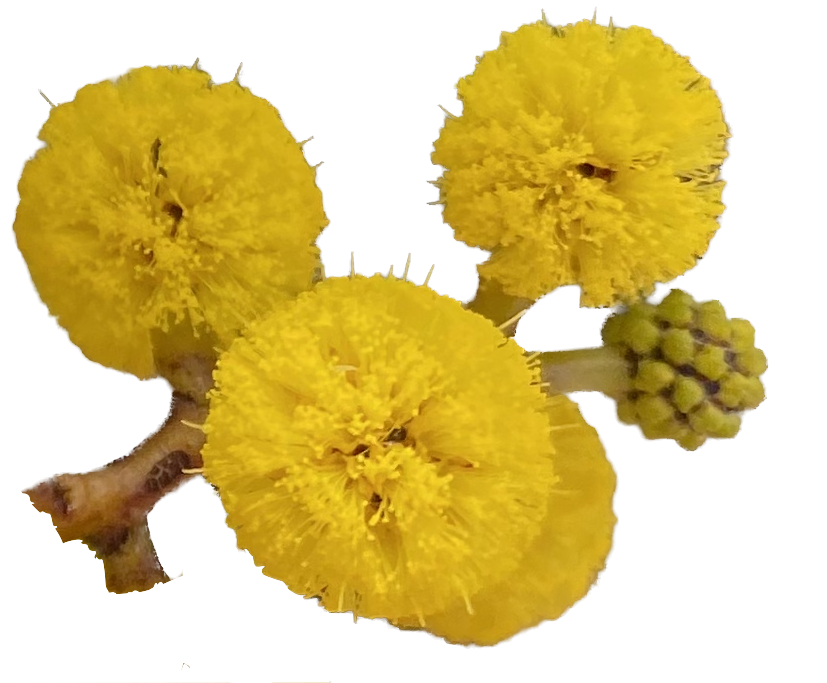
\includegraphics[width=1.5cm]{images/mulga-flowers2.png} % Adjust the image size as needed
    \end{minipage}%
    \hfill % Horizontal space between image and text
    \begin{minipage}[c]{0.8\linewidth} % Adjust width as needed for the text
      \bigskip%
      \textsf{#1}%
      \bigskip%
    \end{minipage}%
    \hspace*{3mm}%
  \end{minipage}%
}%
}
\usepackage{booktabs}
\usepackage{caption}
\usepackage{longtable}
\usepackage{colortbl}
\usepackage{array}
\usepackage{multirow}
\usepackage{wrapfig}
\usepackage{float}
\usepackage{pdflscape}
\usepackage{tabu}
\usepackage{threeparttable}
\usepackage{threeparttablex}
\usepackage[normalem]{ulem}
\usepackage{makecell}
\usepackage{xcolor}
\usepackage{amsmath}
\usepackage{blkarray}
\usepackage[most]{tcolorbox}
\usepackage{xcolor}
\definecolor{info}{HTML}{CBC988}
\definecolor{infostripe}{HTML}{EAC024}
\definecolor{insight}{HTML}{E87C00}
\definecolor{grey}{RGB}{192, 192, 192}
\usepackage{imakeidx}
\makeindex
\usepackage{float}
\floatplacement{table}{H}
\makeatletter
\@ifpackageloaded{bookmark}{}{\usepackage{bookmark}}
\makeatother
\makeatletter
\@ifpackageloaded{caption}{}{\usepackage{caption}}
\AtBeginDocument{%
\ifdefined\contentsname
  \renewcommand*\contentsname{Table of contents}
\else
  \newcommand\contentsname{Table of contents}
\fi
\ifdefined\listfigurename
  \renewcommand*\listfigurename{List of Figures}
\else
  \newcommand\listfigurename{List of Figures}
\fi
\ifdefined\listtablename
  \renewcommand*\listtablename{List of Tables}
\else
  \newcommand\listtablename{List of Tables}
\fi
\ifdefined\figurename
  \renewcommand*\figurename{Figure}
\else
  \newcommand\figurename{Figure}
\fi
\ifdefined\tablename
  \renewcommand*\tablename{Table}
\else
  \newcommand\tablename{Table}
\fi
}
\@ifpackageloaded{float}{}{\usepackage{float}}
\floatstyle{ruled}
\@ifundefined{c@chapter}{\newfloat{codelisting}{h}{lop}}{\newfloat{codelisting}{h}{lop}[chapter]}
\floatname{codelisting}{Listing}
\newcommand*\listoflistings{\listof{codelisting}{List of Listings}}
\makeatother
\makeatletter
\makeatother
\makeatletter
\@ifpackageloaded{caption}{}{\usepackage{caption}}
\@ifpackageloaded{subcaption}{}{\usepackage{subcaption}}
\makeatother
\makeatletter
\@ifpackageloaded{fontawesome5}{}{\usepackage{fontawesome5}}
\makeatother

\usepackage{bookmark}

\IfFileExists{xurl.sty}{\usepackage{xurl}}{} % add URL line breaks if available
\urlstyle{same} % disable monospaced font for URLs
\hypersetup{
  pdftitle={Interactively exploring high-dimensional data and models in R},
  pdfauthor={Dianne Cook and Ursula Laa},
  colorlinks=true,
  linkcolor={blue},
  filecolor={Maroon},
  citecolor={Blue},
  urlcolor={Blue},
  pdfcreator={LaTeX via pandoc}}


\title{Interactively exploring high-dimensional data and models in R}
\author{Dianne Cook and Ursula Laa}
\date{2025-02-18}

\begin{document}
\maketitle

\renewcommand*\contentsname{Contents}
{
\hypersetup{linkcolor=}
\setcounter{tocdepth}{2}
\tableofcontents
}

\bookmarksetup{startatroot}

\chapter*{Preface}\label{preface}

\markboth{Preface}{Preface}

It is important to visualise your data because you might discover things
that you could never have anticipated. Although there are many resources
available for data visualisation, there are few comprehensive resources
on high-dimensional data visualisation. High-dimensional (or
multivariate) data arises when many different things are measured for
each observation. While we can learn many things from plotting with 1D
and 2D or 3D methods there are likely more structures hidden in the
higher dimensions. This book provides guidance on visualising
high-dimensional data and models using linear projections, with R.

High-dimensional data spaces are fascinating places. You may think that
there's a lot of ways to plot one or two variables, and a lot of types
of patterns that can be found. You might use a density plot and see
skewness or a dot plot to find outliers. A scatterplot of two variables
might reveal a non-linear relationship or a barrier beyond which no
observations exist. We don't as yet have so many different choices of
plot types for high-dimensions, but these types of patterns are also
what we seek in scatterplots of high-dimensional data. The additional
dimensions can clarify these patterns, that clusters are likely to be
more distinct. Observations that did not appear to be very different can
be seen to be lonely anomalies in high-dimensions, that no other
observations have quite the same combination of values.

\section*{What's in this book?}\label{whats-in-this-book}
\addcontentsline{toc}{section}{What's in this book?}

\markright{What's in this book?}

The book can be divided into these parts:

\begin{itemize}
\tightlist
\item
  \textbf{Introduction}: Here we introduce you to high-dimensional
  spaces, how they can be visualised, and notation that is useful for
  describing methods in later chapters.\\
\item
  \textbf{Dimension reduction}: This part covers linear and non-linear
  dimension reduction. It includes ways to help decide on the number of
  dimensions needed to summarise the high dimensional data, whether
  linear dimension reduction is appropriate, detecting problems that
  might affect the dimension reduction, and examining how well or badly
  a non-linear dimension reduction is representing the data.
\item
  \textbf{Cluster analysis}: This part described methods for finding
  groups in data. Although it includes an explanation of a purely
  graphical approach, it is mostly on using graphics in association with
  numerical clustering algorithms. There are explanations of assessing
  the suitability of different numerical techniques for extracting
  clusters, based on the data shapes, evaluating the clustering result,
  and showing the solutions in high dimensions.
\item
  \textbf{Classification}: This part describes methods for exploring
  known groups in the data. You'll learn how to check model assumptions,
  to help decide if a method is suited to the data, examine
  classification boundaries and explore where errors arise.
\end{itemize}

In each of these parts an emphasis is also showing your model with your
data in the high dimensional space.

Our hopes are that you will come away with understanding the importance
of plotting your high dimensional data as a regular step in your
statistical or machine learning analyses. There are many examples of
what you might miss if you don't plot the data. Effective use of
graphics goes hand-in-hand with analytical techniques. With high
dimensions visualisation is a challenge but it is fascinating, and leads
to many surprising moments.

\section*{Audience}\label{audience}
\addcontentsline{toc}{section}{Audience}

\markright{Audience}

High-dimensional data arises in many fields such as biology, social
sciences, finance, and more. Anyone who is doing exploratory data
analysis and model fitting for more than two variables will benefit from
learning how to effectively visualise high-dimensions. This book will be
useful for students and teachers of multivariate data analysis and
machine learning, and researchers, data analysts, and industry
professionals who work in these areas.

\section*{How to use the book?}\label{how-to-use-the-book}
\addcontentsline{toc}{section}{How to use the book?}

\markright{How to use the book?}

The book provides explanations and plots accompanied by R code. We would
hope that you run the code to explore the examples as you read the
explanations. The chapters are organised by types of analysis and focus
on how to use the high-dimensional visualisation to complement the
commonly used analytical methods. An overview of the primary
high-dimensional visualisation methods discussed in the book and how to
get started is provided in the toolbox chapter in the Appendix.

The PDF version of the book has many static plots replacing the animated
gifs and interactive plots available in the HTML version. This is
indicated in the figure caption by the \faIcon{play-circle} symbol.

\section*{What should I know before reading this
book?}\label{what-should-i-know-before-reading-this-book}
\addcontentsline{toc}{section}{What should I know before reading this
book?}

\markright{What should I know before reading this book?}

The examples assume that you already use R, and have a working knowledge
of base R and tidyverse way of thinking about data analysis. It also
assumes that you have some knowledge of statistical methods, and some
experience with machine learning methods.

If you feel like you need build up your skills in these areas in
preparation for working through this book, these are our recommended
resources:

\begin{itemize}
\tightlist
\item
  \href{https://r4ds.had.co.nz}{R for Data Science} by Wickham and
  Grolemund for learning about data wrangling and visualisation.
\item
  \href{https://openintro-ims.netlify.app}{Introduction to Modern
  Statistics} by Çetinkaya-Rundel and Hardin to learn about introductory
  statistics.
\item
  \href{https://bradleyboehmke.github.io/HOML/}{Hands-On Machine
  Learning with R} by Boehmke and Greenwell to learn about machine
  learning.
\item
  \href{https://www.tmwr.org}{Tidy Modeling with R} by Kuhn and Silge to
  learn how to tidily do machine learning.
\end{itemize}

We will assume you know how to plot your data and models in 2D. Our
material starts from 2D and beyond.

\section*{Setting up your workflow}\label{setting-up-your-workflow}
\addcontentsline{toc}{section}{Setting up your workflow}

\markright{Setting up your workflow}

To get started set up your computer with the current versions of
\href{https://cran.r-project.org}{R} and ideally also with
\href{https://posit.co/download/rstudio-desktop/}{Rstudio Desktop}.

The examples are created using the
\href{http://ggobi.github.io/tourr/}{\texttt{tourr}} and
\href{https://casperhart.github.io/detourr/}{\texttt{detourr}} packages.
In addition, we have made an R package to share most of the data and
functions used in this book, called
\href{http://dicook.github.io/mulgar}{\texttt{mulgar}}.\footnote{The
  mulga is an iconic landscape in Australia. It is a woodland dominated
  by the mulga tree (Acacia aneura). As you travel through mulga the
  trees look very regular, sometimes like a stand of lollipops, which is
  apparently due to close neighbours being clones! The wood is
  especially hardy, durable and resistant to pests. The climate is
  semi-arid and it can be found across Australia, Queensland, New South
  Wales, South Australia and Western Australia. This landscape is host
  to numerous species: red kangaroos, spinifex hopping mice, mulga
  parrots, dunnarts, thorny devils, bearded dragons, and pests like
  feral goats. Here \textbf{mulgar} is an acronym for
  \textbf{MUL}tivariate \textbf{G}raphical \textbf{A}nalysis with
  \textbf{R}.}\footnote{Photo of mulga tree taken by L. G. Cook.}
Ideally the methods described are not entirely bound by the current
available packages, and still applicable as new technology arises.

\begin{Shaded}
\begin{Highlighting}[]
\FunctionTok{install.packages}\NormalTok{(}\StringTok{"tourr"}\NormalTok{, }\AttributeTok{dependencies=}\ConstantTok{TRUE}\NormalTok{)}
\FunctionTok{install.packages}\NormalTok{(}\StringTok{"detourr"}\NormalTok{, }\AttributeTok{dependencies=}\ConstantTok{TRUE}\NormalTok{)}
\FunctionTok{install.packages}\NormalTok{(}\StringTok{"mulgar"}\NormalTok{, }\AttributeTok{dependencies=}\ConstantTok{TRUE}\NormalTok{)}
\end{Highlighting}
\end{Shaded}

and development versions can be installed from the GitHub repositories
for the packages. To get a copy of the code and additional data used and
an RStudio project to get started, you can download with this code:

\begin{Shaded}
\begin{Highlighting}[]
\NormalTok{u }\OtherTok{\textless{}{-}} \StringTok{"https://dicook.github.io/mulgar\_book/code\_and\_data.zip"}
\NormalTok{usethis}\SpecialCharTok{::}\FunctionTok{use\_zip}\NormalTok{(}\AttributeTok{url=}\NormalTok{u)}
\end{Highlighting}
\end{Shaded}

You will be able to click on the \texttt{mulgar\_book.Rproj} to get
started with the code.

\section*{Suggestion, feedback or
error?}\label{suggestion-feedback-or-error}
\addcontentsline{toc}{section}{Suggestion, feedback or error?}

\markright{Suggestion, feedback or error?}

We welcome suggestions, feedback or details of errors. You can report
them as an issue at the
\href{https://github.com/dicook/mulgar_book}{Github repo for this book}.

Please make a small \href{https://reprex.tidyverse.org}{reproducible
example} and report the error encountered. Reproducible examples have
these components:

\begin{itemize}
\tightlist
\item
  a small amount of data
\item
  small amount of code that generates the error
\item
  copy of the error message that was generated
\end{itemize}

\part{Introduction}

\chapter{Picturing high dimensions}\label{intro}

High-dimensional data means that we have a large number of features or
variables, which can be considered as dimensions in a mathematical
space. The variables can be different types, such as categorical or
temporal, but the handling of these variables involves different
techniques. Here we focus on primarily numeric variables, which might be
considered as belonging to a Euclidean space where each observation is a
vector and the distance between observations can be described by a
distance metric. \index{dimensionality} \index{variable}\index{feature}
\index{Euclidean space} \index{distance metric} \index{vector}

Models that operate on high-dimensional data can be thought of as
decomposing observations into two sets of values, fitted values and
residuals from the fit. The fitted values capture the systematic or
predictable variation between variables, and can be considered a
sharpened view of the data, to see through the noise in the data. The
residuals capture this noise, and represent random variation. When using
models for high-dimensional data, such as unsupervised or supervised
classification, or dimension reduction, it is important to use
visualisation to assess how well the model fits the data. If it fits
well, picturing the model fit might be a clearer view of the
relationships between variables. \index{model!fitted values}
\index{model!residuals}

\begin{figure}

\centering{

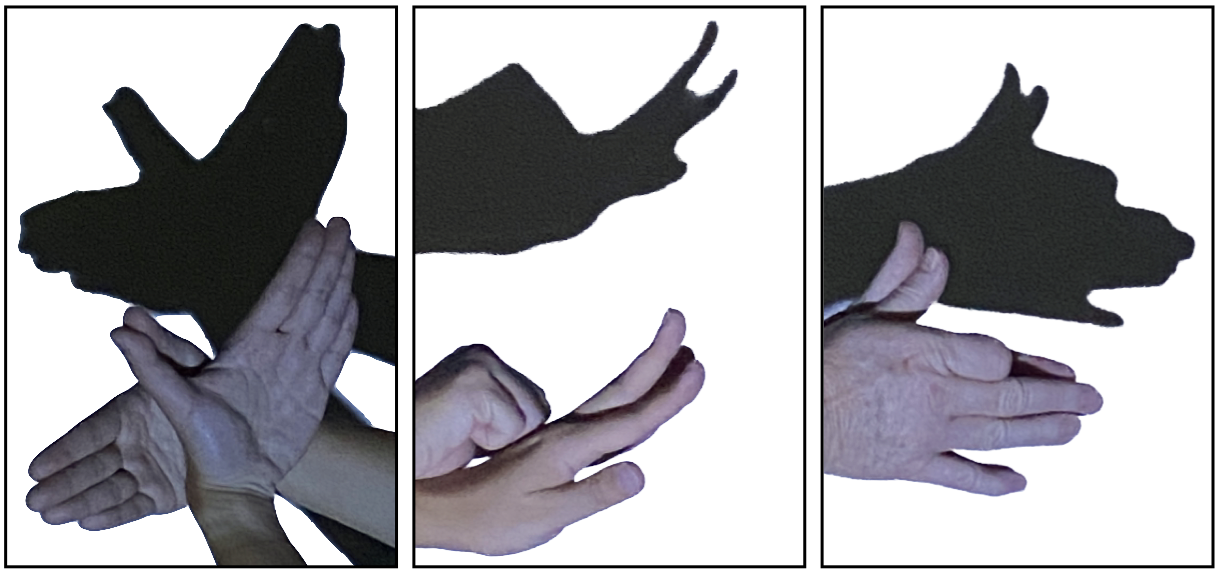
\includegraphics[width=4.6875in,height=\textheight,keepaspectratio]{images/shadow_puppets.png}

}

\caption{\label{fig-shadow-puppets}Viewing high dimensions using
low-dimensional displays is like playing shadow puppets, looking at the
shadows to guess what the shape is.}

\end{figure}%

One approach to visualise numeric high dimensional data and models is by
using linear projections, as done in a tour (Asimov, 1985; Buja \&
Asimov, 1986; Cook et al., 2006; S. Lee et al., 2022). You can think of
projections of high-dimensional data like shadows
(Figure~\ref{fig-shadow-puppets}). Unlike shadow puppets, though the
object stays fixed, and with multiple projections we can obtain a
\emph{view of the object from all sides}. A tour will pick directions to
look at by selecting a set of linear projections. The views are
interpolated to move from one linear projection to the next, this is
displayed as an animation. \index{projection} \index{shadow}

\infobox{With a tour we slowly rotate the viewing direction, this allows us to see many individual projections and to track movement patterns. Look for interesting structures such as clusters or outlying points.}

\section{Getting familiar with tours}\label{getting-familiar-with-tours}

\begin{figure*}

\centering{

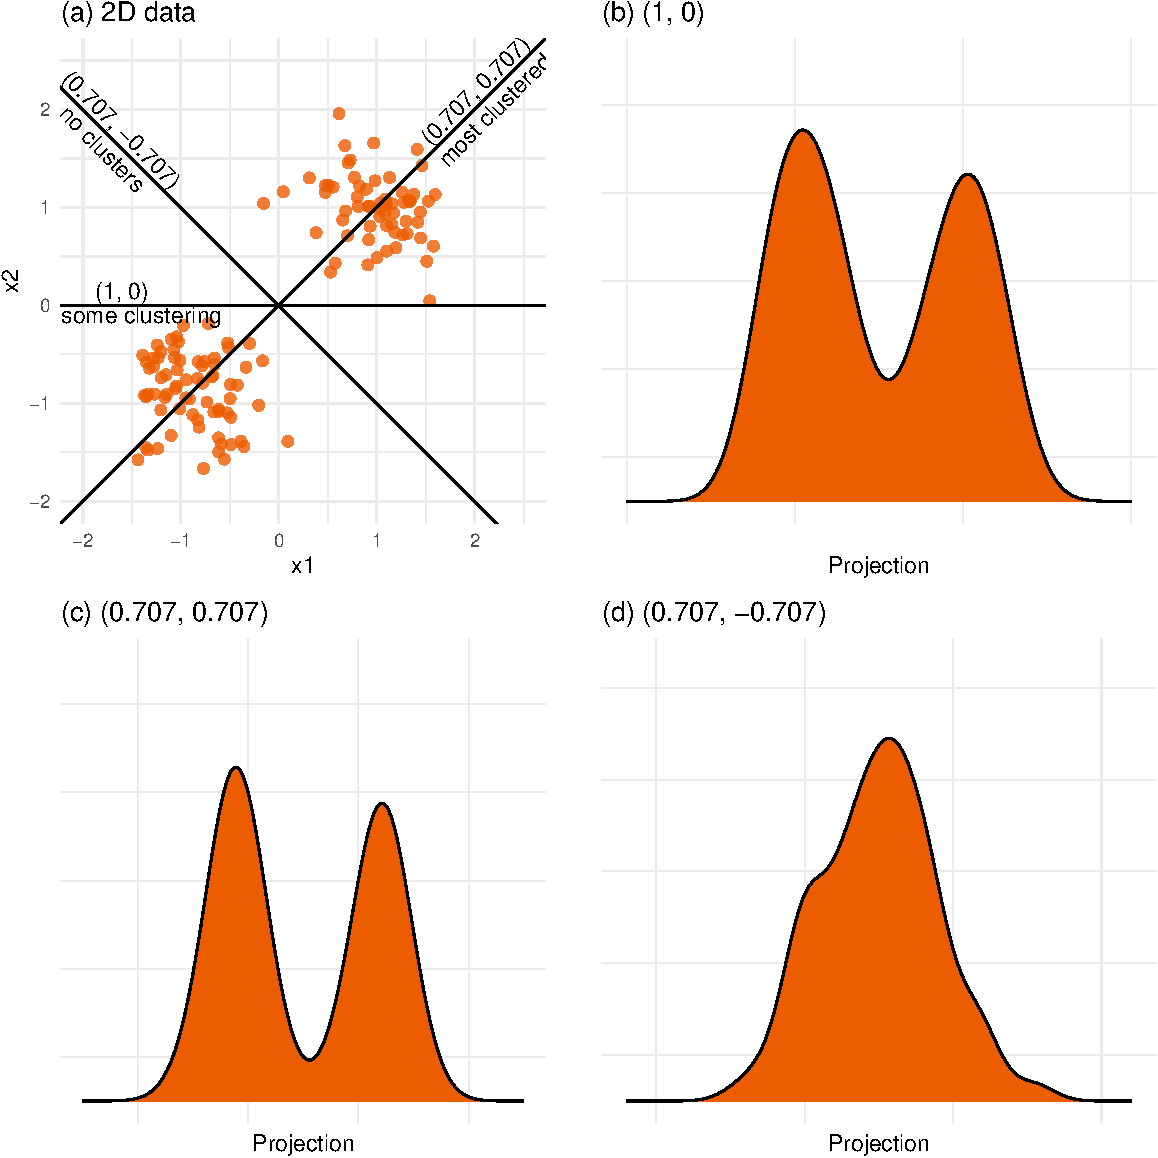
\includegraphics[width=1\linewidth,height=\textheight,keepaspectratio]{1-intro_files/figure-pdf/fig-explain-1D-pdf-1.pdf}

}

\caption{\label{fig-explain-1D-pdf}How a tour can be used to explore
high-dimensional data illustrated using (a) 2D data with two clusters
and (b,c,d) 1D projections from a tour shown as a density plot. Imagine
spinning a line around the centre of the data plot, with points
projected orthogonally onto the line. With this data, when the line is
at \texttt{x1=x2\ (0.707,\ 0.707)} or \texttt{(-0.707,\ -0.707)} the
clustering is the strongest. When it is at
\texttt{x1=-x2\ \ (0.707,\ -0.707)} there is no clustering.
\faIcon{play-circle}}

\end{figure*}%

Figure~\ref{fig-explain-1D-pdf} illustrates a tour for 2D data and 1D
projections. The (grand) tour will generate all possible 1D projections
of the data, and display with a univariate plot like a histogram or
density plot. For this data, the \texttt{simple\_clusters} data,
depending on the projection, the distribution might be clustered into
two groups (bimodal), or there might be no clusters (unimodal). In this
example, all projections are generated by rotating a line around the
centre of the plot. Clustering can be seen in many of the projections,
with the strongest being when the contribution of both variables is
equal, and the projection is \texttt{(0.707,\ \ 0.707)} or
\texttt{(-0.707,\ -0.707)}. (If you are curious about the number
\texttt{0.707}, the Chapter~\ref{sec-notation} provides the
explanation.) \index{projection!1D} \index{tour!grand}

\begin{figure*}

\centering{

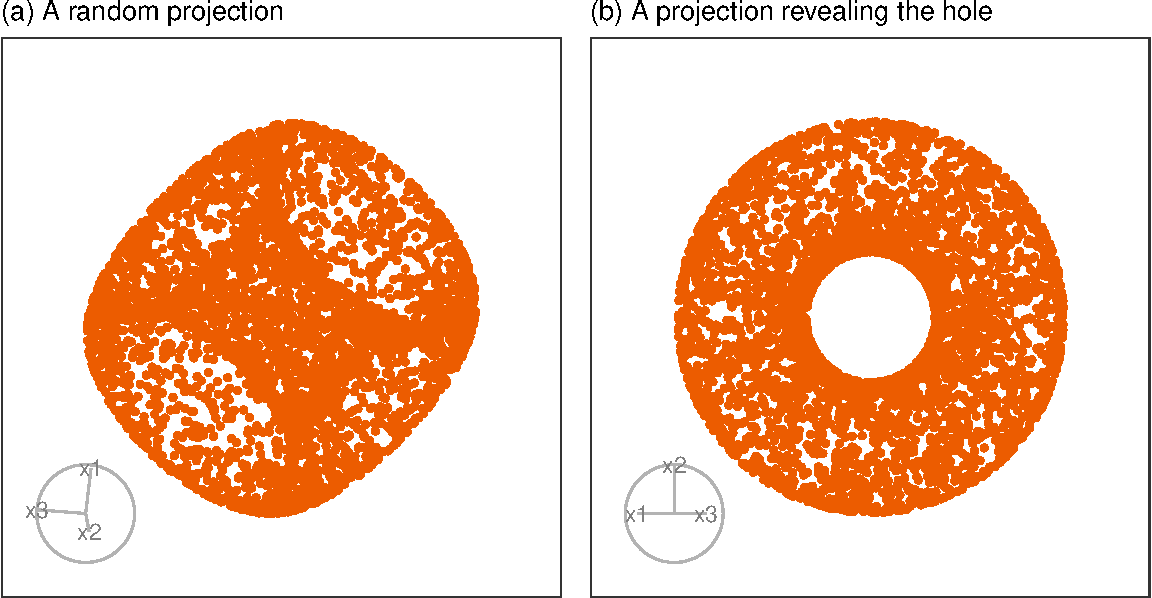
\includegraphics[width=1\linewidth,height=\textheight,keepaspectratio]{1-intro_files/figure-pdf/fig-explain-2D-pdf-1.pdf}

}

\caption{\label{fig-explain-2D-pdf}How a tour can be used to explore
high-dimensional data illustrated by showing a sequence of random 2D
projections of 3D data (a). The data has a donut shape with the hole
revealed in a single 2D projection (b). Data usually arrives with a
given number of observations, and when we plot it like this using a
scatterplot, it is like shadows of a transparent object.
\faIcon{play-circle}}

\end{figure*}%

Figure~\ref{fig-explain-2D-pdf} illustrates a tour for 3D data using 2D
projections. The data are points on the surface of a donut shape. By
showing the projections using a scatterplot the donut looks transparent
and we can see through the data. The donut shape can be inferred from
watching many 2D projections but some are more revealing that others.
The projection shown in (b) is where the hole in the donut is clearly
visible. \index{projection!2D}

\section{Reading the axes}\label{reading-the-axes}

The coefficients of the projection are important to matching the
variables with the patterns detected. For example, in the 2D data used
in Figure~\ref{fig-explain-1D-pdf} the primary structure to detect is
the clustering. It is when a positive, equal combination of the two
variables \texttt{x1} and \texttt{x2} are used that the two clusters can
be observed in a projection.

When the projection dimension is 2, as in the example data used in
Figure~\ref{fig-explain-2D-pdf}, there are two sets of projection
coefficients. These are represented in the plot by the circle and line
segments. The direction and length of the line segments indicate how the
variable contributes to the view seen. Lining these up with any patterns
in the data helps to understand how the variables contribute to making
the pattern. In this data, the interesting feature is the hole in the
donut, which can be seen in certain combinations of \texttt{x1} and
\texttt{x3} plotted against \texttt{x2}.

\section{What's different about space beyond
2D?}\label{whats-different-about-space-beyond-2d}

The term ``high-dimensional'' in this book refers to the dimensionality
of the Euclidean space. Figure~\ref{fig-dimension-cubes} shows a way to
imagine this. It shows a sequence of cube wireframes, ranging from
one-dimensional (1D) through to five-dimensional (5D), where beyond 2D
is a linear projection of the cube. As the dimension increases, a new
orthogonal axis is added. For cubes, this is achieved by doubling the
cube: a 2D cube consists of two 1D cubes, a 3D cube consists of two 2D
cubes, and so forth. This is a great way to think about the space being
examined by the visual methods, and also all of the machine learning
methods mentioned, in this book.

\index{dimensionality}

\begin{figure}

\centering{

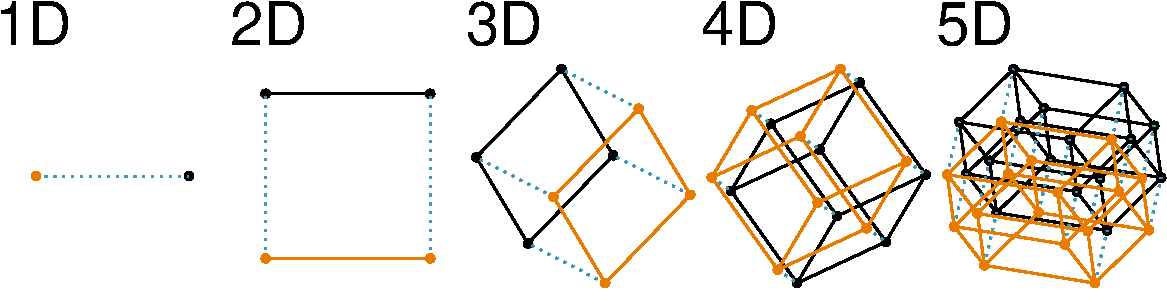
\includegraphics[width=0.8\linewidth,height=\textheight,keepaspectratio]{1-intro_files/figure-pdf/fig-dimension-cubes-1.pdf}

}

\caption{\label{fig-dimension-cubes}Space can be considered to be a
high-dimensional cube. Here we have pictured a sequence of increasing
dimension cubes, from 1D to 5D, as wireframes, it can be seen that as
the dimension increase by one, the cube doubles.}

\end{figure}%

Interestingly, the struggle with imagining high-dimensions this way is
described in a novel titled ``Flatland: A Romance of Many Dimensions''
published in 1884 (Abbott, 1884) \footnote{Thanks to Barret Schloerke
  for directing co-author Cook to this history when he was an
  undergraduate student and we were starting the
  \href{http://schloerke.com/geozoo/}{geozoo} project.}. Yes, more than
100 years ago! This is a story about characters living in a 2D world,
being visited by an alien 3D character. It also is a social satire,
serving the reader strong messages about gender inequity, although this
provides the means to explain more intricacies in perceiving dimensions.
There have been several movies made based on the book in recent decades
(e.g. Martin (1965), D. Johnson \& Travis (2007)). Although purchasing
the movies may be prohibitive, watching the trailers available for free
online is sufficient to gain enough geometric intuition on the nature of
understanding high-dimensional spaces while living in a low-dimensional
world.

When we look at high-dimensional spaces from a low-dimensional space, we
meet the ``curse of dimensionality'', a term introduced by Bellman
(1961) to express the difficulty of doing optimization in high
dimensions because of the exponential growth in space as dimension
increases. A way to imagine this is look at the cubes in
Figure~\ref{fig-dimension-cubes}: As you go from 1D to 2D, 2D to 3D, the
space expands a lot, and imagine how vast space might get as more
dimensions are added\footnote{``Space is big. Really big. You might
  think it's a long way to the pharmacy, but that's peanuts to space.''
  from Douglas Adams'
  \href{https://en.wikipedia.org/wiki/The_Hitchhiker\%27s_Guide_to_the_Galaxy\#Stage_shows}{Hitchhiker's
  Guide to the Galaxy} always springs to mind when thinking about high
  dimensions!}. The volume of the space grows exponentially with
dimension, which makes it infeasible to sample enough points -- any
sample will be less densely covering the space as dimension increases.
The effect is that most points will be far from the sample mean, on the
edge of the sample space.

\index{dimensionality!curse of}

For visualisation, the curse manifests in an opposite manner. Projecting
from high to low dimensions creates a crowding or piling of points near
the center of the distribution. This was noted by Diaconis \& Freedman
(1984a). Figure~\ref{fig-density} illustrates this phenomenon, using
samples that are uniformly distributed in \(p\)-dimensional spheres. As
dimension increases, the points crowd the centre, even with as few as
ten dimensions. This is something that we may need to correct for when
exploring high dimensions with low-dimensional projections.

\index{dimensionality!crowding}

\begin{figure}

\centering{

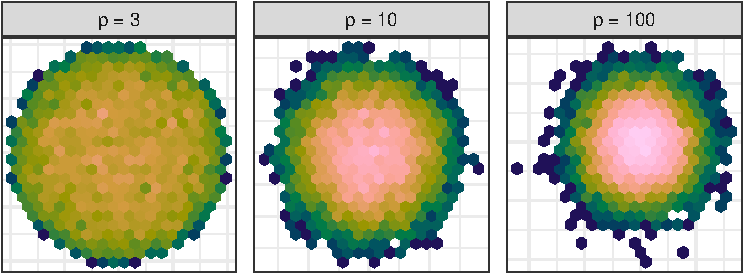
\includegraphics[width=0.95\linewidth,height=\textheight,keepaspectratio]{1-intro_files/figure-pdf/fig-density-1.pdf}

}

\caption{\label{fig-density}Illustration of data crowding in the
low-dimensional projection as dimension increases, here from 3, 10, 100.
The samples are generated from a uniform distribution in
\(p\)-dimensional spheres. Colour shows the number of points in each
hexagon bin (pink is large, navy is small). As dimension increases the
points concentrate near the centre.}

\end{figure}%

Figure~\ref{fig-tour-intro-pdf} shows 2D tours of two different 5D data
sets. One has clusters (a) and the other has two outliers and a plane
(b). Can you see these? One difference in the viewing of data with more
than three dimensions with 2D projections is that the points seem to
shrink towards the centre, and then expand out again. This the effect of
dimensionality, with different variance or spread in some directions.

\begin{figure}

\begin{minipage}{0.50\linewidth}

\centering{

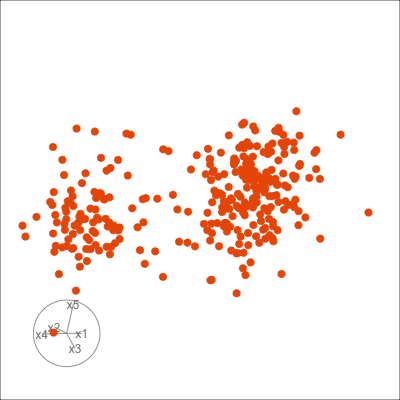
\includegraphics[width=2.08333in,height=\textheight,keepaspectratio]{images/clusters-intro.png}

}

\subcaption{\label{fig-tour-clusters}Clusters}

\end{minipage}%
%
\begin{minipage}{0.50\linewidth}

\centering{

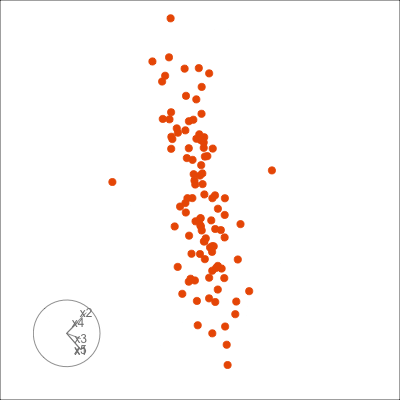
\includegraphics[width=2.08333in,height=\textheight,keepaspectratio]{images/outlier-intro.png}

}

\subcaption{\label{fig-tour-clusters}Outliers}

\end{minipage}%

\caption{\label{fig-tour-intro-pdf}Frames from 2D tours on two 5D
datasets, with clusters of points in (a) and two outliers with a plane
in (b). \faIcon{play-circle}}

\end{figure}%

\section{What can you learn?}\label{what-can-you-learn}

There are two ways of detecting structure in tours:

\begin{itemize}
\tightlist
\item
  patterns in a single low-dimensional projection
\item
  movement patterns
\end{itemize}

with the latter being especially useful when displaying the projected
data as a scatterplot. Figure~\ref{fig-example-structure} shows examples
of patterns we typically look for when making a scatterplot of data.
These include clustering, linear and non-linear association, outliers,
barriers where there is a sharp edge beyond which no observations are
seen. Not shown, but it also might be possible to observe multiple
modes, or density of observations, L-shapes, discreteness or uneven
spread of points. The tour is especially useful if these patterns are
only visible in combinations of variables.

\begin{figure}

\centering{

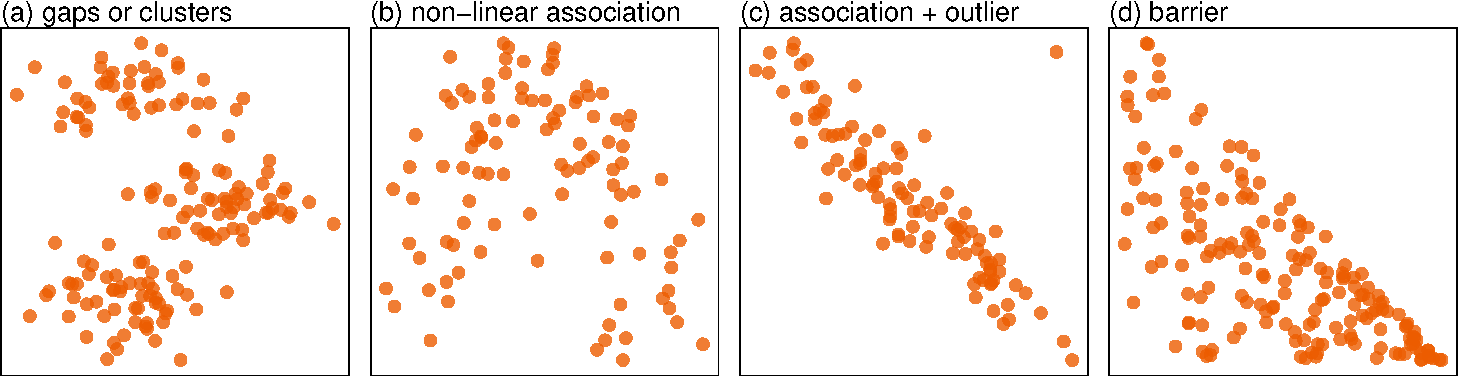
\includegraphics[width=1\linewidth,height=\textheight,keepaspectratio]{1-intro_files/figure-pdf/fig-example-structure-1.pdf}

}

\caption{\label{fig-example-structure}Example structures that might be
visible in a 2D projection that imply presence of structure in high
dimensions. These include clusters, linear and non-linear association,
outliers and barriers.}

\end{figure}%

Figure~\ref{fig-trails} illustrates how movement patterns of points when
using scatterplots to display 2D projections indicate clustering (a, b)
and outliers (c, d).

\begin{figure}

\begin{minipage}{0.50\linewidth}

\centering{

\pandocbounded{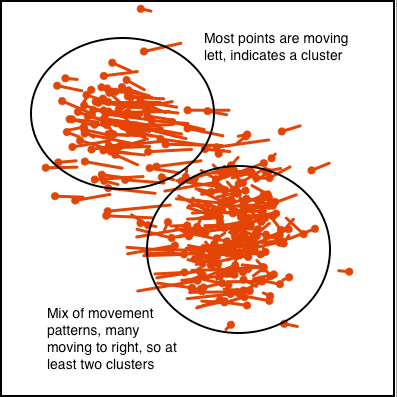
\includegraphics[keepaspectratio]{images/trails-clusters.png}}

}

\subcaption{\label{fig-clusters-trails-static}Clustering}

\end{minipage}%
%
\begin{minipage}{0.50\linewidth}

\centering{

\pandocbounded{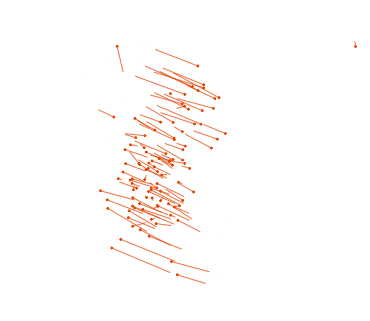
\includegraphics[keepaspectratio]{images/trails-outlier.png}}

}

\subcaption{\label{fig-outlier-trails-static}Outliers}

\end{minipage}%

\caption{\label{fig-trails}The movement of points give further clues
about the structure of the data in high-dimensions. In the data with
clustering, often we can see a group of points moving differently from
the others. Because there are three clusters, you should see three
distinct movement patterns. It is similar with outliers, except these
may be individual points moving alone, and different from all others.
This can be seen in the static plot, one point (top left) has a movement
pattern upwards whereas most of the other observations near it are
moving down towards the right.}

\end{figure}%

This type of visualisation is useful for many activities in dealing with
high-dimensional data, including:

\begin{itemize}
\tightlist
\item
  exploring high-dimensional data.
\item
  detecting if the data lives in a lower dimensional space than the
  number of variables.
\item
  checking assumptions required for multivariate models to be
  applicable.
\item
  check for potential problems in modeling such as multicollinearity
  among predictors.
\item
  checking assumptions required for probabilities calculated for
  statistical hypothesis testing to be valid.
\item
  diagnosing the fit of multivariate models.
\end{itemize}

\infobox{You use a tour when analysing multivariate data so that you can see what exists in the data and what your models are fitting, in the same way that you walk down the street with {\em your eyes open} to avoid being hit by a bus or to discover a delightful shop.}

\section{A little history}\label{a-little-history}

Viewing high-dimensional data based on low-dimensional projections can
probably be traced back to the early work on principal component
analysis by Pearson (1901) and Hotelling (1933), which was extended to
known classes as part of discriminant analysis by Fisher (1936a).

With computer graphics, the capability of animating plots to show more
than a single best projection became possible. The video library (ASA
Statistical Graphics Section, 2023) is the best place to experience the
earliest work. Kruskal's 1962 animation of multidimensional scaling
showed the process of finding a good 2D representation of high
dimensional data, although the views are not projections. Chang's 1970
video shows her rotating a high dimensional point cloud along coordinate
axes to find a special projection where all the numbers align. The
classic video that must be watched is PRIM9 (Fisherkeller et al., 1973)
where a variety of interactive and dynamic tools are used together to
explore high dimensional physics data, documented in Fisherkeller et al.
(1974).

The methods in this book primarily emerge from Asimov (1985)'s grand
tour method. The algorithm provided the first smooth and continuous
sequence of low dimensional projections, and guaranteed that all
possible low dimensional projections were likely to be shown. The
algorithm was refined in Buja \& Asimov (1986) (and documented in detail
in Buja et al. (2005)) to make it \emph{efficiently} show all possible
projections. Since then there have been numerous varieties of tour
algorithms developed to focus on specific tasks in exploring high
dimensional data, and these are documented in S. Lee et al. (2022).

This book is an evolution from Cook \& Swayne (2007). One of the
difficulties in working on interactive and dynamic graphics research has
been the rapid change in technology. Programming languages have changed
a little (FORTRAN to C to java to python) but graphics toolkits and
display devices have changed a lot! The tour software used in this book
evolved from XGobi, which was written in C and used the X Window System,
which was then rewritten in GGobi using gtk. The video library has
engaging videos of these software systems. There have been several other
short-lived implementations, including orca (Sutherland et al., 2000a),
written in java, and cranvas (Xie et al., 2014), written in R with a
back-end provided by wrapper functions to \texttt{qt} libraries.

Although attempts were made with these ancestor systems to connect the
data plots to a statistical analysis system, these were always limited.
With the emergence of R, having graphics in the data analysis workflow
has been much easier, albeit at the cost of the interactivity with
graphics that matches the old systems. We are mostly using the R
package, \texttt{tourr} (Wickham et al., 2011a) for examples in this
book. It provides the machinery for running a tour, and has the
flexibility that it can be ported, modified, and used as a regular
element of data analysis.

\section{An illustration of the
benefits}\label{an-illustration-of-the-benefits}

The Palmer penguins data (A. M. Horst et al., 2022) is available in the
R package \texttt{palmerpenguins} (A. Horst et al., 2022). These are
measurements on three species of penguins, recording the bill length
(\texttt{bl}) and depth (\texttt{bd}), flipper length (\texttt{fl}) and
body mass (\texttt{bm}), along with the sex, island location and year of
recording. Of interest here are the four physical measurements and the
species. There are two penguins with missing values on these
measurements which are removed from the analysis below. The variables
have also been standardised. \index{data!penguins}

\begin{figure}

\centering{

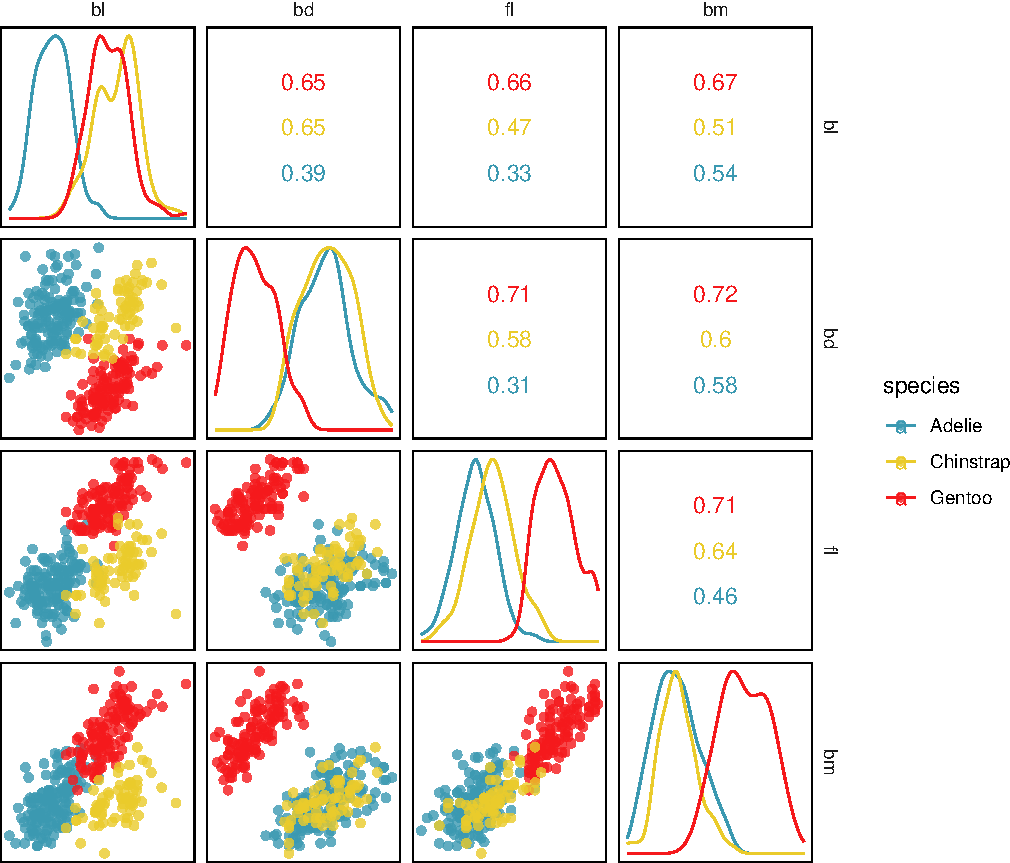
\includegraphics[width=1\linewidth,height=\textheight,keepaspectratio]{1-intro_files/figure-pdf/fig-penguins-scatmat-1.pdf}

}

\caption{\label{fig-penguins-scatmat}Scatterplot matrix of the penguins,
with colour indicating the three species, Adelie, Chinstrap, Gentoo. The
clusters for each species are similarly shaped in each scatterplot, and
centred at different locations in some plots.}

\end{figure}%

Figure~\ref{fig-penguins-scatmat} shows the data as a scatterplot
matrix, as produced by the \texttt{ggscatmat} function in the R package
GGally (Emerson et al., 2013), a common way to examine multivariate data
with low-dimensional plots: pairwise scatterplots and univariate density
plots. A lot of information can be gained from viewing this plot:

\begin{itemize}
\tightlist
\item
  the three species form three clusters, indicating that the physical
  characteristics of the three are different.
\item
  the Gentoo species forms a separated cluster when \texttt{bd} is
  plotted with \texttt{bm}.
\item
  there is one anomaly, a Chinstrap penguin that has a very low value of
  \texttt{fl} relative to it's \texttt{bl} measurement.
\end{itemize}

Although one cannot see it in this plot clearly, making the plot larger
also reveals that \texttt{fl} values appear to have been often rounded
because there is some discreteness in the plots.

\begin{figure}

\begin{minipage}{0.50\linewidth}

\pandocbounded{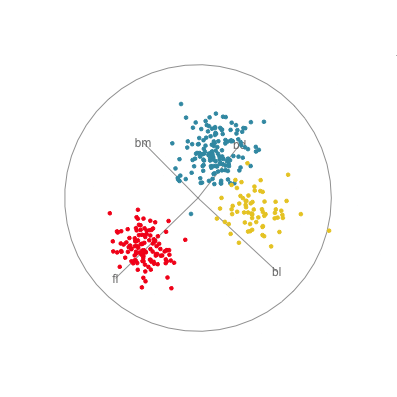
\includegraphics[keepaspectratio]{images/penguins6.png}}

\subcaption{\label{}Nice view}
\end{minipage}%
%
\begin{minipage}{0.50\linewidth}

\pandocbounded{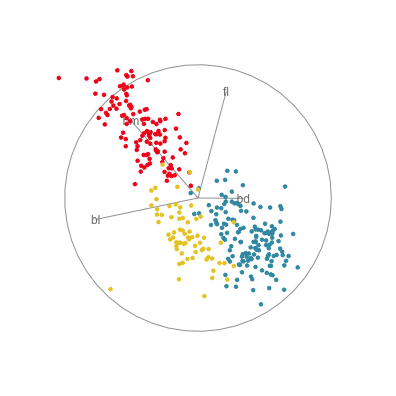
\includegraphics[keepaspectratio]{images/penguins5.png}}

\subcaption{\label{}Chinstrap anomaly}
\end{minipage}%
\newline
\begin{minipage}{0.50\linewidth}

\pandocbounded{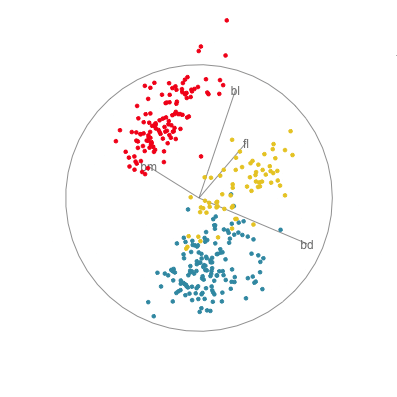
\includegraphics[keepaspectratio]{images/penguins3.png}}

\subcaption{\label{}Gentoo anomaly}
\end{minipage}%
%
\begin{minipage}{0.50\linewidth}

\pandocbounded{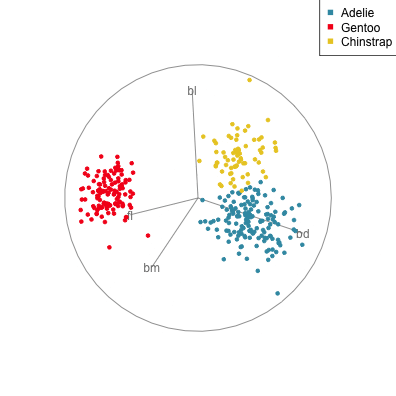
\includegraphics[keepaspectratio]{images/penguins4.png}}

\subcaption{\label{}Multiple anomalies}
\end{minipage}%

\caption{\label{fig-penguins-tour}Four projections from a tour, showing
the data \emph{from more sides}. We can see that the separation between
clusters is larger and that there are more unusually shaped penguins.}

\end{figure}%

In Figure~\ref{fig-penguins-tour} there are four 2D projections from a
grand tour of the penguins data. Projection (a) reveals a 2D projection
where all three species are distinct. It's quite a nice view where all
species have circular spread, the Gentoo are separated, and the other
two are very slightly overlapped. There is also one Adelie penguin that
is a little different from the others here, primarily due to having
large flippers but small bill depth. Projection (b) shows the anomalous
Chinstrap penguin, and reveals that the gap between it and the other
penguins is bigger than was seen in the scatterplot matrix. Projection
(c) shows that there is an unusual Gentoo penguin, and projection (d)
shows possibly a few more anomalous Gentoo, with relatively small
\texttt{bl} and larger \texttt{bm}.

In terms of understanding how the variables contribute to the patterns
observed, we need to study the axes display on each plot. In projection
(a) showing the nice view of the clusters, all four variables contribute
in an interesting way. The variables operate in pairs of what we might
call contrasts in statistics: \texttt{bl} and \texttt{bm} combine in the
top left to bottom right direction, while \texttt{fl} and \texttt{bd}
combine in the top right to bottom left direction. Because the axes are
pointing in opposite directions, in each pair one variable contributes
in the opposite way to the other. That is, one coefficient in the pair
will be positive and the other negative. We can also infer that
\texttt{fl} and \texttt{bd} contribute most to distinguishing Gentoo
from the other species, and also that \texttt{bl} and \texttt{bm}
contribute primarily to distinguishing Chinstrap from Adelie penguins.

Interpretations can be checked against plots of the individual
variables, like the scatterplot matrix in
Figure~\ref{fig-penguins-scatmat}. Here, can see that, yes, \texttt{bl}
is primarily distinguishing Chinstrap from Adelie, and \texttt{fl}
strongly contributes to distinguishing Gentoo from the others. The plot
of \texttt{bl} against \texttt{fl} has a reasonably good view of the
three species as different from each other. This view gets even better
when \texttt{bm} is combined with \texttt{bl}, and \texttt{bd} is
combined with \texttt{fl}, to produce what we see with the tour.

The penguins data is relatively simple, and well-studied. Despite this,
examining this data with a tour of linear projections provides a few
more details that may have gone unobserved.

\section{Common choices of tours}\label{common-choices-of-tours}

There are many different types of tours, all generated by different ways
of choosing the sequence of linear projections to show. There are three
main ones we commonly use, grand tour, guided tour and manual or radial
tour. The grand tour is designed to show as many projections of the data
as fast as possible with the goal being to give an overview or big
picture of the data. The guided tour is used when particular patterns,
such as clusters or anomalies, need to be discovered. It steers the
choice of projections towards those that have these patterns. The radial
tour a variable (or combination of two) from the projection, then puts
it back, with the specific intent to learn if the pattern depends on
this variable's contribution. If the pattern disappears when the
variable disappears it means that this variable is vital or very
important for defining the pattern.

The Appendix~\ref{sec-toolbox} contains details on running tours,
primarily using the \texttt{tourr} package but other software is listed.
A grand tour making 2D projections uses the \texttt{animate\_xy()}
function, which implicitly uses the algorithm created by the
\texttt{grand\_tour()} function. The guided tour is created using the
\texttt{guided\_tour()} function as an argument, and the radial/manual
tour is created using the \texttt{radial\_tour()} function as an
argument. It is also useful to use the \texttt{save\_history()} function
to pre-compute the set of projections to show, and then use the
\texttt{planned\_tour()} function to play the sequence. All the
different algorithms for generating paths of projections can be used
with \texttt{save\_history()}. For saving an animation to include in an
HTML document the \texttt{render\_gif()} can be used. It will save a set
of images to a file that will be recognised as an animated gif. It is
also possible to extract any of the individual images from this file.
All the gifs accompanying this book are created using the
\texttt{render\_gif()} function.

\section{Do you really have high-dimensional
data?}\label{do-you-really-have-high-dimensional-data}

Even though, you have multiple numeric variables, there may not be any
need to use high-dimensional data visualisation. The purpose of using
high-dimensional visualisation is to learn about the associations
between variables. If there is no association between variables
everything we need to learn can be done with univariate data
visualisation methods. Chapter~\ref{sec-dimension-overview} focuses on
this dimensionality, finding associations, and reducing dimensionality.

\begin{figure}[H]

{\centering 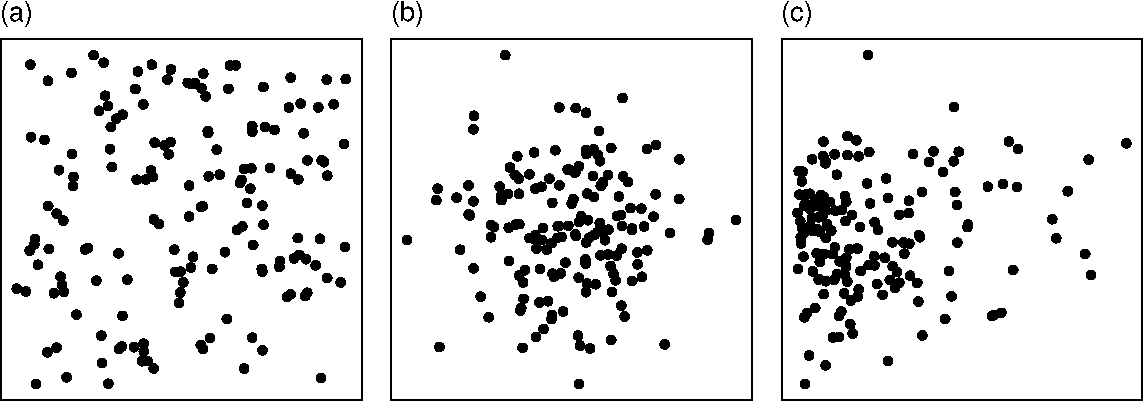
\includegraphics[width=1\linewidth,height=\textheight,keepaspectratio]{1-intro_files/figure-pdf/do-you-have-high-d-1.pdf}

}

\caption{Examples of 2D data that lack association, for which univariate
methods are sufficient: (a) points spread uniformly in the square, (b)
points spread in a circle with higher density in the middle, (c) points
conentrated in the centre vertically and skewed to the right.}

\end{figure}%

\section*{Exercises}\label{exercises}
\addcontentsline{toc}{section}{Exercises}

\markright{Exercises}

\begin{enumerate}
\def\labelenumi{\arabic{enumi}.}
\tightlist
\item
  Randomly generate data points that are uniformly distributed in a
  hyper-cube of 3, 5 and 10 dimensions, with 500 points in each sample,
  using the \texttt{cube.solid.random()} function of the \texttt{geozoo}
  package. What differences do we expect to see? Now visualise each set
  in a grand tour and describe how they differ, and whether this matched
  your expectations?
\item
  Use the \texttt{geozoo} package to generate samples from different
  shapes and use them to get a better understanding of how shapes appear
  in a grand tour. You can start with exploring the conic spiral in 3D,
  a torus in 4D and points along the wire frame of a cube in 5D.
\item
  For each of the challenge data sets, \texttt{c1}, \ldots, \texttt{c7}
  from the \texttt{mulgar} package, use the grand tour to view and try
  to identify structure (outliers, clusters, non-linear relationships).
\item
  The \texttt{datasets} package in R has some classic data to explore.

  \begin{enumerate}
  \def\labelenumii{\alph{enumii}.}
  \tightlist
  \item
    Examine the \texttt{USArrests} data, using a grand tour
    (\texttt{animate\_xy()}). Explain the structure, and why the scale
    of the variables might affect your interpretation of the structure.
    Re-run the tour on standardised variables (option
    \texttt{recale=TRUE}). Do you see any outliers?
  \item
    Examine the \texttt{swiss} data, using a grand tour, making sure to
    use standardised variables. Explain the patterns that you see.
  \end{enumerate}
\item
  The \texttt{MASS} package has two data sets that are interesting to
  examine.

  \begin{enumerate}
  \def\labelenumii{\alph{enumii}.}
  \tightlist
  \item
    Using a grand tour of the physical variables (\texttt{FL},
    \texttt{RW}, \texttt{CL}, \texttt{CW}, \texttt{BD}) variables in the
    \texttt{crabs} data with the points coloured by species
    (\texttt{sp}) what can you see? Is there a difference in the
    species? (Note that for this data you don't need to standardise. All
    are measured in the same units, and are not too different in scale,
    so the associations can still be seen well enough.)
  \item
    Using a grand tour of the chemical \% (\texttt{Na}:\texttt{Fe})
    variables in the \texttt{fgl} data with the points coloured by
    \texttt{type} what can you see? Is there a difference in the types
    of glass? (Here, the variables need to be standardised. Even though
    they are \%'s, the different amounts of each impede the ability to
    assess the associations without rescaling.)
  \end{enumerate}
\item
  There are several interesting data sets available on the
  \href{http://ggobi.org/book/index.html}{GGobi website}, for example,
  one of Tukey's original data set \texttt{PRIM7}. Examine this data for
  different types of patterns. The \texttt{olive}, \texttt{PBC}, and
  \texttt{music} data sets are also interesting to explore.
  \texttt{PRIM7} can be read using:
\end{enumerate}

\begin{Shaded}
\begin{Highlighting}[]
\FunctionTok{library}\NormalTok{(readr)}
\NormalTok{prim7 }\OtherTok{\textless{}{-}} \FunctionTok{read\_csv}\NormalTok{(}\StringTok{"http://ggobi.org/book/data/prim7.csv"}\NormalTok{,}
                  \AttributeTok{show\_col\_types =} \ConstantTok{FALSE}\NormalTok{)}
\end{Highlighting}
\end{Shaded}

\section*{Project}\label{project}
\addcontentsline{toc}{section}{Project}

\markright{Project}

The data set \texttt{nigeria-water-imputed.csv} contains water
availability data recorded for Nigeria, obtained from
https://www.waterpointdata.org. Examining this data is motivated by an
analysis by Julia Silge
\href{https://juliasilge.com/blog/water-sources/}{``Predict availability
in \#TidyTuesday water sources with random forest models''}. The data
has been cleaned, and a small number of missing values have been imputed
using the variable means. Variables with \texttt{\_NA} at the end
indicate values that are imputed, and can be ignored for this exercise.

\begin{enumerate}
\def\labelenumi{\arabic{enumi}.}
\tightlist
\item
  There are 86684 observations. To do an initial examination of the the
  data we will start with a small subset. Make a 1\% sample to work
  with. Note, that generally when sampling one should sample the same
  fraction within strata that are important for the analysis. Here we
  will examine the type of water source as indicated by the
  \texttt{water\_tech\_category} variable. You can do the sampling with
  this code:
\end{enumerate}

\begin{Shaded}
\begin{Highlighting}[]
\FunctionTok{library}\NormalTok{(tidyverse)}
\FunctionTok{library}\NormalTok{(tourr)}
\NormalTok{water }\OtherTok{\textless{}{-}} \FunctionTok{read\_csv}\NormalTok{(}\StringTok{"data/nigeria{-}water{-}imputed.csv"}\NormalTok{)}
\FunctionTok{set.seed}\NormalTok{(}\DecValTok{113}\NormalTok{)}
\NormalTok{water\_sub }\OtherTok{\textless{}{-}}\NormalTok{ water }\SpecialCharTok{|\textgreater{}}
  \FunctionTok{group\_by}\NormalTok{(water\_tech\_category) }\SpecialCharTok{|\textgreater{}}
  \FunctionTok{sample\_frac}\NormalTok{(}\AttributeTok{size =} \FloatTok{0.01}\NormalTok{)}
\end{Highlighting}
\end{Shaded}

\begin{enumerate}
\def\labelenumi{\arabic{enumi}.}
\setcounter{enumi}{1}
\tightlist
\item
  Take a look at the variables starting with \texttt{distance\_}. This
  can be done more easily by making a smaller subset of variables (see
  code below, and using shorter variable names). What are the patterns
  you can see? Does it look like there is much association between
  variables, or clustering?
\end{enumerate}

\begin{Shaded}
\begin{Highlighting}[]
\NormalTok{water\_dist }\OtherTok{\textless{}{-}}\NormalTok{ water\_sub }\SpecialCharTok{|\textgreater{}}
  \FunctionTok{select}\NormalTok{(water\_tech\_category, }\FunctionTok{starts\_with}\NormalTok{(}\StringTok{"distance"}\NormalTok{)) }\SpecialCharTok{|\textgreater{}}
  \FunctionTok{select}\NormalTok{(}\SpecialCharTok{!}\FunctionTok{contains}\NormalTok{(}\StringTok{"\_NA"}\NormalTok{)) }\SpecialCharTok{|\textgreater{}}
  \FunctionTok{mutate}\NormalTok{(}\AttributeTok{water\_tech\_category =} \FunctionTok{factor}\NormalTok{(water\_tech\_category)) }\SpecialCharTok{|\textgreater{}}
  \FunctionTok{rename}\NormalTok{(}\AttributeTok{dpr =}\NormalTok{ distance\_to\_primary\_road,}
         \AttributeTok{dsr =}\NormalTok{ distance\_to\_secondary\_road,}
         \AttributeTok{dtr =}\NormalTok{ distance\_to\_tertiary\_road,}
         \AttributeTok{dc =}\NormalTok{ distance\_to\_city,}
         \AttributeTok{dt =}\NormalTok{ distance\_to\_town)}
\FunctionTok{animate\_xy}\NormalTok{(water\_dist[,}\DecValTok{2}\SpecialCharTok{:}\DecValTok{6}\NormalTok{], }\AttributeTok{rescale=}\ConstantTok{TRUE}\NormalTok{)}
\end{Highlighting}
\end{Shaded}

\begin{enumerate}
\def\labelenumi{\arabic{enumi}.}
\setcounter{enumi}{2}
\tightlist
\item
  Now let's see how the type of water source might vary by distance.
  Colour the points by the \texttt{water\_tech\_category} and examine
  this in a grand tour. Would you expect that the water source is
  different depending on the distance from populated areas?
\end{enumerate}

\begin{Shaded}
\begin{Highlighting}[]
\FunctionTok{animate\_xy}\NormalTok{(water\_dist[,}\DecValTok{2}\SpecialCharTok{:}\DecValTok{6}\NormalTok{], }\AttributeTok{rescale=}\ConstantTok{TRUE}\NormalTok{,}
           \AttributeTok{col=}\NormalTok{water\_dist}\SpecialCharTok{$}\NormalTok{water\_tech\_category)}
\end{Highlighting}
\end{Shaded}

\begin{enumerate}
\def\labelenumi{\arabic{enumi}.}
\setcounter{enumi}{3}
\tightlist
\item
  Now try using a guided tour to find the best combination to see the
  differences between the type of water sources. Interpret which
  variable combination yields this difference.
\end{enumerate}

\begin{Shaded}
\begin{Highlighting}[]
\FunctionTok{set.seed}\NormalTok{(}\DecValTok{324}\NormalTok{)}
\FunctionTok{animate\_xy}\NormalTok{(water\_dist[,}\DecValTok{2}\SpecialCharTok{:}\DecValTok{6}\NormalTok{],}
           \FunctionTok{guided\_tour}\NormalTok{(}\FunctionTok{lda\_pp}\NormalTok{(water\_dist}\SpecialCharTok{$}\NormalTok{water\_tech\_category)),}
           \AttributeTok{rescale=}\ConstantTok{TRUE}\NormalTok{,}
           \AttributeTok{col=}\NormalTok{water\_dist}\SpecialCharTok{$}\NormalTok{water\_tech\_category)}
\end{Highlighting}
\end{Shaded}

\chapter{Technical details}\label{sec-notation}

\section{Notation conventions and R
objects}\label{notation-conventions-and-r-objects}

The data can be considered to be a matrix of numbers with the columns
corresponding to variables, and the rows correspond to observations. It
can be helpful to write this in mathematical notation, like:

\begin{eqnarray*}
X_{n\times p} =
[X_1~X_2~\dots~X_p]_{n\times p} = \left[ \begin{array}{cccc}
X_{11} & X_{12} & \dots & X_{1p} \\
X_{21} & X_{22} & \dots & X_{2p}\\
\vdots & \vdots &  & \vdots \\
X_{n1} & X_{n2} & \dots & X_{np} \end{array} \right]_{n\times p}
\end{eqnarray*}

where \(X\) indicates the \(n\times p\) data matrix, \(X_j\) indicates
variable \(j, j=1, \dots, p\) and \(X_{ij}\) indicates the value of the
\(j^{th}\) variable for the \(i^{th}\) observation. (It can be confusing
to distinguish whether one is referring to the observation or a
variable, because \(X_i\) is used to indicate observation. In
descriptions where it is unclear we will use \(X_{i.}\) to indicate
observation/row and \(X_{.j}\) to indicate variable/column. Also this
will usually accompanied by qualifying words such as
\textbf{observation} or \textbf{variable}.)

\index{data!matrix}

\infobox{Having notation is helpful for concise explanations of different methods, to explain how data is scaled, processed and projected for various tasks, and how different quantities are calculated from the data. }

When there is a response variable(s), it is common to consider \(X\) to
be the predictors, and use \(Y\) to indicate the response variable(s).
\(Y\) could be a matrix, also, and would be \(n\times q\), where
commonly \(q=1\). \(Y\) could be numeric or categorical, and this would
change how it is handled with visualisation.

To make a low-dimensional projection (shadow) of the data onto \(d\)
dimensions (\(d < p\)), we need an orthonormal basis:

\begin{eqnarray*}
A_{p\times d} = \left[ \begin{array}{cccc}
A_{11} & A_{12} & \dots & A_{1d} \\
A_{21} & A_{22} & \dots & A_{2d}\\
\vdots & \vdots &  & \vdots \\
A_{p1} & A_{p2} & \dots & A_{pd} \end{array} \right]_{p\times d}
\end{eqnarray*}

\index{orthonormal} \index{projection basis}

\(A\) should be an orthonormal matrix, which means that the
\(\sum_{j=1}^p A_{jk}^2=1, k=1, \dots, d\) (columns represent vectors of
length 1) and \(\sum_{j=1}^p A_{jk}A_{jl}=0, k,l=1, \dots, d; k\neq l\)
(columns represent vectors that are orthogonal to each other). In matrix
notation, this can be written as \(A^{\top}A = I_d\).
\index{data!projection}

Then the projected data is written as:

\begin{eqnarray*}
Y_{n\times d} = XA = \left[ \begin{array}{cccc}
y_{11} & y_{12} & \dots & y_{1d} \\
y_{21} & y_{22} & \dots & y_{2d}\\
\vdots & \vdots &  & \vdots \\
y_{n1} & y_{n2} & \dots & y_{nd} \end{array} \right]_{n\times d}
\end{eqnarray*}

where \(y_{ij} = \sum_{k=1}^p X_{ik}A_{kj}\). Note that we are using
\(Y\) as the projected data here, as well as it possibly being used for
a response variable. Where necessary, this will be clarified with words
in the text, when notation is used in explanations later.

When using R, if we only have the data corresponding to \(X\) it makes
sense to use a \texttt{matrix} object. However, if the response variable
is included and it is categorical, then we might use a
\texttt{data.frame} or a \texttt{tibble} which can accommodate
non-numerical values. Then to work with the data, we can use the base R
methods:

\begin{Shaded}
\begin{Highlighting}[]
\NormalTok{X }\OtherTok{\textless{}{-}} \FunctionTok{matrix}\NormalTok{(}\FunctionTok{c}\NormalTok{(}\FloatTok{1.1}\NormalTok{, }\FloatTok{1.3}\NormalTok{, }\FloatTok{1.4}\NormalTok{, }\FloatTok{1.2}\NormalTok{, }
              \FloatTok{2.7}\NormalTok{, }\FloatTok{2.6}\NormalTok{, }\FloatTok{2.4}\NormalTok{, }\FloatTok{2.5}\NormalTok{, }
              \FloatTok{3.5}\NormalTok{, }\FloatTok{3.4}\NormalTok{, }\FloatTok{3.2}\NormalTok{, }\FloatTok{3.6}\NormalTok{), }
            \AttributeTok{ncol=}\DecValTok{4}\NormalTok{, }\AttributeTok{byrow=}\ConstantTok{TRUE}\NormalTok{)}
\NormalTok{X}
\end{Highlighting}
\end{Shaded}

\begin{verbatim}
     [,1] [,2] [,3] [,4]
[1,]  1.1  1.3  1.4  1.2
[2,]  2.7  2.6  2.4  2.5
[3,]  3.5  3.4  3.2  3.6
\end{verbatim}

which is a data matrix with \(n=3, p=4\) and to extract a column
(variable):

\begin{Shaded}
\begin{Highlighting}[]
\NormalTok{X[,}\DecValTok{2}\NormalTok{]}
\end{Highlighting}
\end{Shaded}

\begin{verbatim}
[1] 1.3 2.6 3.4
\end{verbatim}

or a row (observation):

\begin{Shaded}
\begin{Highlighting}[]
\NormalTok{X[}\DecValTok{2}\NormalTok{,]}
\end{Highlighting}
\end{Shaded}

\begin{verbatim}
[1] 2.7 2.6 2.4 2.5
\end{verbatim}

or an individual cell (value):

\begin{Shaded}
\begin{Highlighting}[]
\NormalTok{X[}\DecValTok{3}\NormalTok{,}\DecValTok{2}\NormalTok{]}
\end{Highlighting}
\end{Shaded}

\begin{verbatim}
[1] 3.4
\end{verbatim}

To make the data projection we need an orthonormal matrix:

\begin{Shaded}
\begin{Highlighting}[]
\NormalTok{A }\OtherTok{\textless{}{-}} \FunctionTok{matrix}\NormalTok{(}\FunctionTok{c}\NormalTok{(}\FloatTok{0.707}\NormalTok{,}\FloatTok{0.707}\NormalTok{,}\DecValTok{0}\NormalTok{,}\DecValTok{0}\NormalTok{,}\DecValTok{0}\NormalTok{,}\DecValTok{0}\NormalTok{,}\FloatTok{0.707}\NormalTok{,}\FloatTok{0.707}\NormalTok{), }\AttributeTok{ncol=}\DecValTok{2}\NormalTok{, }\AttributeTok{byrow=}\ConstantTok{FALSE}\NormalTok{)}
\NormalTok{A}
\end{Highlighting}
\end{Shaded}

\begin{verbatim}
      [,1]  [,2]
[1,] 0.707 0.000
[2,] 0.707 0.000
[3,] 0.000 0.707
[4,] 0.000 0.707
\end{verbatim}

You can check that it is orthonormal by

\begin{Shaded}
\begin{Highlighting}[]
\FunctionTok{sum}\NormalTok{(A[,}\DecValTok{1}\NormalTok{]}\SpecialCharTok{\^{}}\DecValTok{2}\NormalTok{)}
\end{Highlighting}
\end{Shaded}

\begin{verbatim}
[1] 0.999698
\end{verbatim}

\begin{Shaded}
\begin{Highlighting}[]
\FunctionTok{sum}\NormalTok{(A[,}\DecValTok{1}\NormalTok{]}\SpecialCharTok{*}\NormalTok{A[,}\DecValTok{2}\NormalTok{])}
\end{Highlighting}
\end{Shaded}

\begin{verbatim}
[1] 0
\end{verbatim}

and compute the projected data using matrix multiplication:

\begin{Shaded}
\begin{Highlighting}[]
\NormalTok{X }\SpecialCharTok{\%*\%}\NormalTok{ A}
\end{Highlighting}
\end{Shaded}

\begin{verbatim}
       [,1]   [,2]
[1,] 1.6968 1.8382
[2,] 3.7471 3.4643
[3,] 4.8783 4.8076
\end{verbatim}

The magical number \texttt{0.707} used above and to create the
projection in Figure~\ref{fig-explain-1D-pdf} arises from normalising a
vector with equal contributions from each variable, \texttt{(1,\ 1)}.
Dividing by \texttt{sqrt(2)} gives \texttt{(0.707,\ 0.707)}.

\infobox{The notation convention used throughout the book is:
\begin{itemize}
\item n = number of observations
\item p = number of variables, dimension of data
\item d = dimension of the projection
\item g = number of groups, in classification
\item X = data matrix
\end{itemize}
}

\section{Mechanics of tours}\label{mechanics-of-tours}

\subsection{Different ways to choose target
bases}\label{different-ways-to-choose-target-bases}

Although there are a variety of different tour types, they are (almost)
all composed of three core building blocks: a set of target projection
bases, a method for interpolating between them and the method to display
the projected data. The manner that the target planes are chosen
primarily determines the type of tour. Figure~\ref{fig-tour-types-pdf}
illustrates three main tour types: grand, guided and radial. The
appendix has a list of the many others.

\infobox{
Tours are composed from three elements:
\begin{itemize}
\item a set of target projection bases
\item an interpolation method
\item the method to display the projected data
\end{itemize}
}

The original tour was called the \emph{grand tour} (Asimov, 1985). In a
grand tour, the target bases are chosen randomly from all possible
projections. The reason to use a grand tour is to get an overview of the
data quickly - it is possible to discover relationships between
variables that were not pre-conceived. The particular grand tour
available in the \texttt{tourr} package also has the feature that all
projections are equally likely to be viewed, and it efficiently covers
the space of all projections. The tour in the \texttt{langevitour}
(Harrison, 2023) software is similar to a grand tour but uses a
different dynamic to choose the tour path, based on jostling particles.
It doesn't need to do interpolation because changes are incremental.

\index{tour!grand} \index{tour!guided}

Because space gets large as dimension increases, the wait for seeing
interesting structure in projections when using a grand tour can be
long. So if you have an idea of the types of structure that would be
interesting to observe using a \emph{guided tour} (Cook et al., 1995a)
may help. A guided tour chooses target bases according to some function
describing interesting, and the tour path follows an optimisation of
this function. For example, the \texttt{LDA} index (E.-K. Lee et al.,
2005) is a function that describes the separation between known classes
in a projection, and is defined as follows:

\begin{eqnarray*}
I_{\rm LDA}(A) = 1- \frac{|A'WA|}{|A'(W+B)A|}
\end{eqnarray*}

where \(B = \sum_{i=1}^g
n_i(\bar{y}_{i.}-\bar{y}_{..})(\bar{y}_{i.}-\bar{y}_{..})',
W=\sum_{i=1}^g\sum_{j=1}^{n_i}
(y_{ij}-\bar{y}_{i.})(y_{ij}-\bar{y}_{i.})'\) are the between- and
within-group sum of squares matrices in a linear discriminant analysis,
with \(g=\)number of groups, and \(n_i, i=1, ....g\) is the number of
cases in each group.

The \emph{radial tour} (Laa et al., 2023) provides a way to assess the
importance of any variable or combination of variables. The target basis
is chosen by zeroing out a variable (or multiple variables) and the
interpolation runs from the initial projection to the target and back to
the initial. If the structure observed in the initial plot doesn't
change much when the variable(s) is removed, then the variable is not
important. This is often best combined with the guided tour, where the
radial tour would start from the best projection (as done in
Figure~\ref{fig-tour-types-pdf} c), the most structured projection, and
each of the variables can be tested for their importance in producing
the structure.

Each of these tour types can be run in the \texttt{tourr} package by
setting the \texttt{tour\_path} parameter of the \texttt{animate\_XXX()}
functions. The paths of projection bases can also be generated and saved
to be used later with the \texttt{save\_history()} function. This is the
manner with which to save a particular data projection, or to generate
sequences of projections to pass to external software.

\begin{figure}

\begin{minipage}{\linewidth}

\pandocbounded{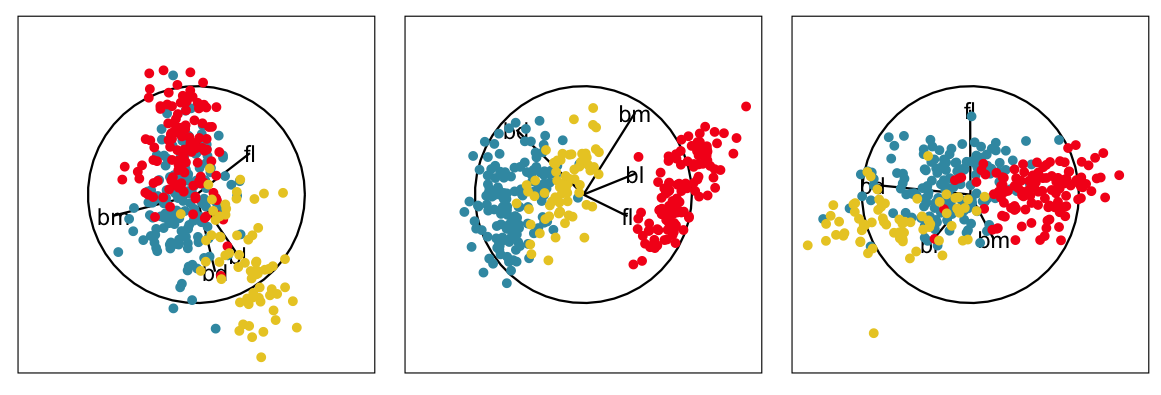
\includegraphics[keepaspectratio]{images/p_grand3.png}}

\subcaption{\label{}Data projected into three target projection bases
from a grand tour}
\end{minipage}%
\newline
\begin{minipage}{\linewidth}

\pandocbounded{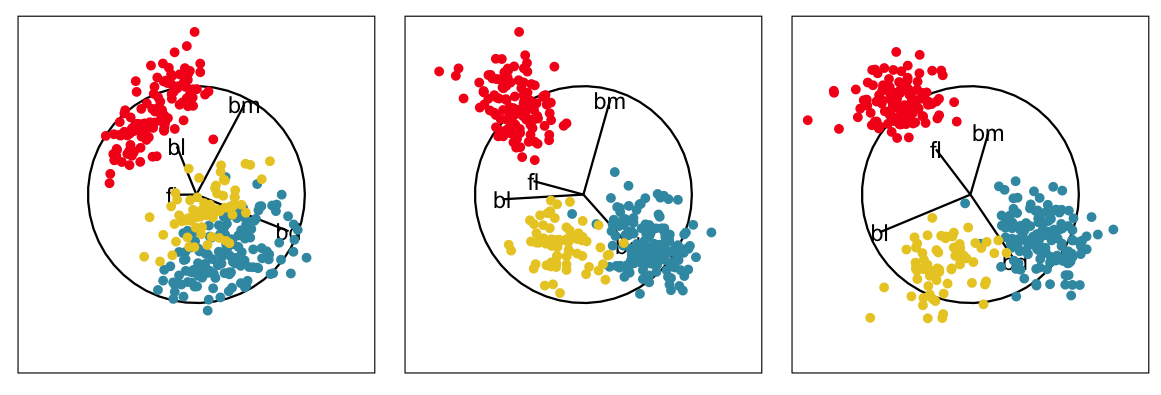
\includegraphics[keepaspectratio]{images/p_guided3.png}}

\subcaption{\label{}Data projected into three target projection bases
from a guided tour}
\end{minipage}%
\newline
\begin{minipage}{\linewidth}

\pandocbounded{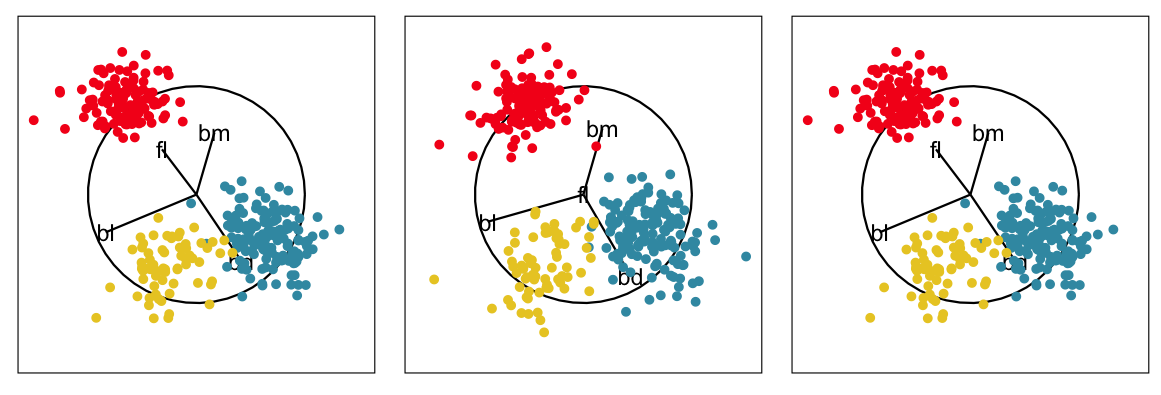
\includegraphics[keepaspectratio]{images/p_radial3.png}}

\subcaption{\label{}Data projected into three target projection bases
from a radial tour}
\end{minipage}%

\caption{\label{fig-tour-types-pdf}With the grand tour (a) each target
plane is randomly selected, to show as many possible projections as
possible and obtain an overview of the data. A tour guided by the LDA
index (b) steers towards projections where the species are most
separated. However, the guided tour might miss something unexpected,
like the anomaly (yellow) seen in the third grand tour frame (a). The
radial tour (c) rotates a variable (here \texttt{fl}) out of the
projection and back in to assess the impact on the structure. It can be
seen that removing the contribution of \texttt{fl} makes only a small
difference to the separation. \faIcon{play-circle}}

\end{figure}%

\begin{figure}

\begin{minipage}{\linewidth}

\pandocbounded{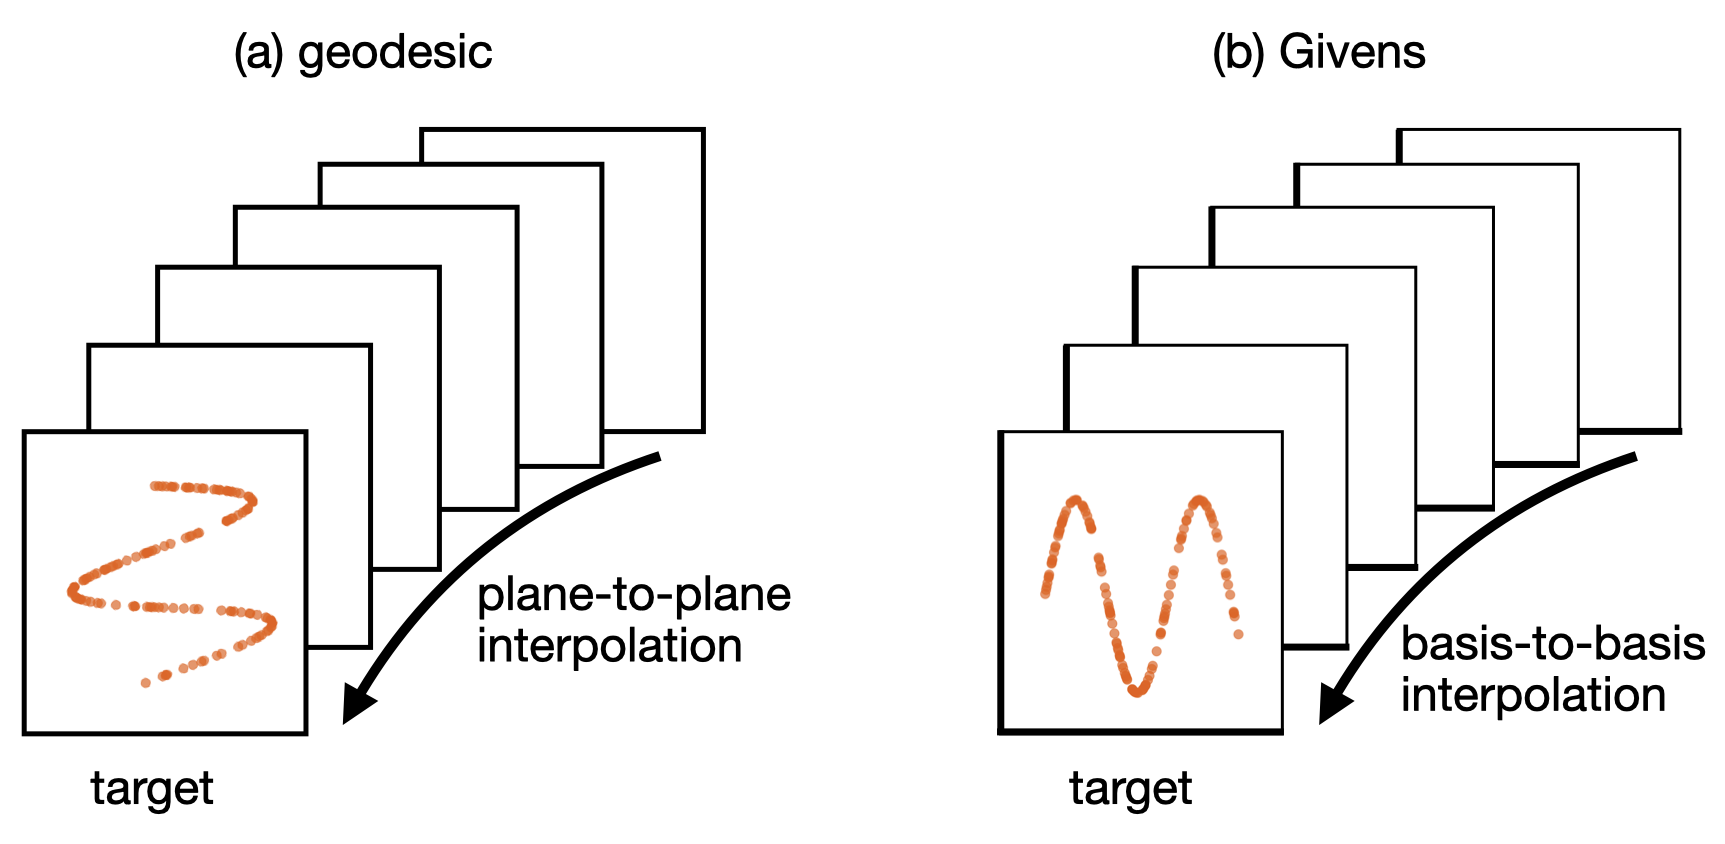
\includegraphics[keepaspectratio]{images/interpolation.png}}

\end{minipage}%

\caption{\label{fig-interpolation}Two different types of interpolation
to a target: (a) geodesic plane-to-plane, (b) basis-to-basis using
Givens rotations. The geodesic interpolation follows the shortest paths
between planes. Givens respects the orientation of the basis when
plotting or calculating projection pursuit indexes. Both methods
maintain orthonormality of the bases for each step.}

\end{figure}%

\subsection{Interpolating between
targets}\label{interpolating-between-targets}

Interpolating from the current basis to the target basis is most
commonly achieved using geodesic interpolation. This type of
interpolation (described in Buja et al. (2005)) has especially important
properties: (1) it is plane-to-plane so follows the shortest path, and
(2) maintains orthonormality of the basis at each step when \(d>1\). The
plane-to-plane movement operates like video stabilisation, by removing
the within-plane spin, so you can focus on structure without distracting
movement. However, when using the guided tour if the index is not
rotationally invariant, for example, if based on correlation or splines,
it can be important respect a particular orientation. For this rare
situation, using Givens interpolation, available in the \texttt{woylier}
package (Batsaikhan et al., 2024) can be helpful.
Figure~\ref{fig-interpolation} illustrates the difference.

\subsection{Displaying the projected
data}\label{displaying-the-projected-data}

Based on the dimension of the projection basis there are natural ways to
display the projected data. If \(d=2\) it is most common that we would
use a scatterplot, as shown in Figure~\ref{fig-tour-types-pdf}.

If \(d=1\) there are many choices of display - histogram, density plot,
dotplot, boxplot - any method commonly used to display univariate
continuous data (see \texttt{animate\_dist()}). If \(d=1\) but a second
(set of) variable(s) is available, such as a time index, a categorical
variable index (\texttt{animate\_idx()}), or spatial coordinates
(\texttt{animate\_image()}), then the display might reserve one axis for
the projected data and another for the additional variables.
Figure~\ref{fig-displays} shows two different display choices for
\(d=1\), a histogram of the projected data (a) and an ordered dotplot of
an index created by combining values of several ranking variables. In
each display the box with horizontal lines at the bottom represents the
projection coefficients. In (a) there are six variables contributing to
the projection, four with negative coefficients, which reveals some
bimodality and a potential anomaly in this data. In (b), nine ranking
variables on the liveability of nine US cities are combined to give an
overall rank for each city. (Data originally from Savageau \& Boyer
(1993).) This combination is a projection, and a tour is used to assess
how the city ranks would change if the combination of these measures
changed. That is, the use case, is how robust is the ranking to small
changes in its construction.

When \(d>2\), even though it primarily academic, some possible choices
are to use stereo to simulate 3D, scatterplot matrices or parallel
coordinates.

\begin{figure}

\begin{minipage}{0.60\linewidth}

\pandocbounded{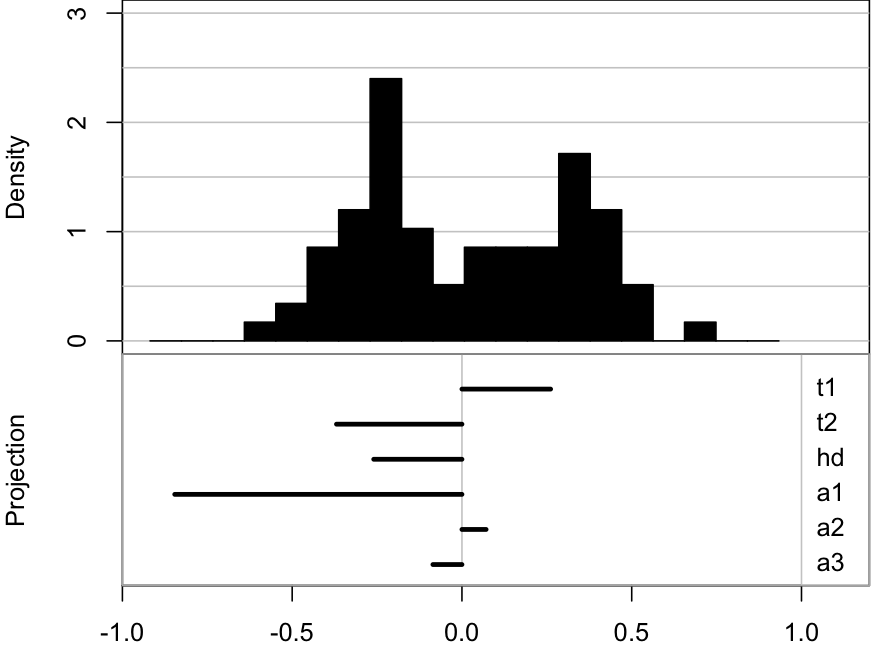
\includegraphics[keepaspectratio]{images/display-dist2.png}}

\subcaption{\label{}histogram}
\end{minipage}%
%
\begin{minipage}{0.40\linewidth}

\pandocbounded{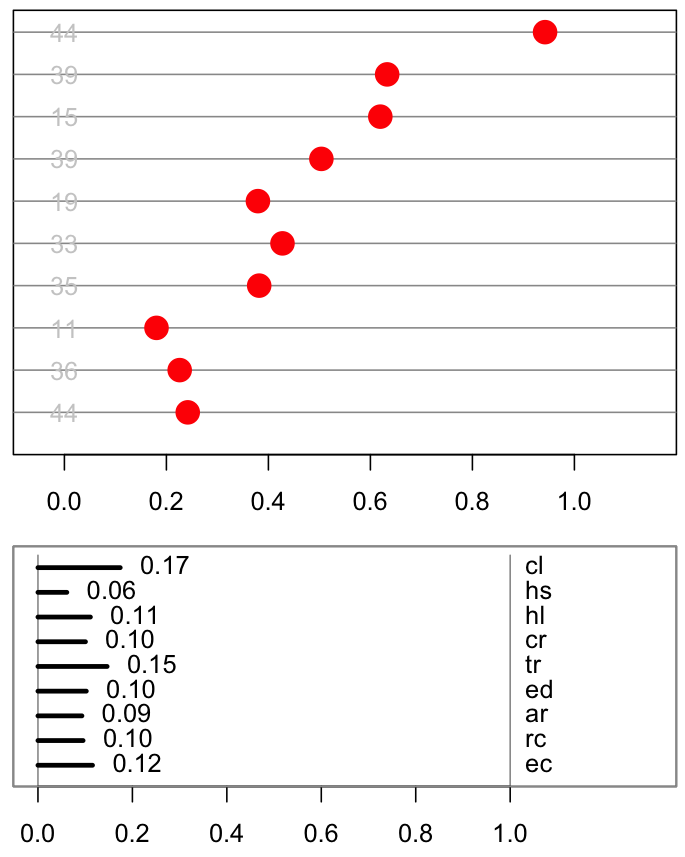
\includegraphics[keepaspectratio]{images/display-idx.png}}

\subcaption{\label{}dotplot}
\end{minipage}%

\caption{\label{fig-displays}Different choices for displaying projected
data: (a) histogram, (b) ordered dotplot. In each case the projected
data is 1D. In the histogram, the lines at the bottom of the display
correspond to the projection basis. For the ordered dotplot, each point
corresponds to a US city which has been measured on several criteria
such as housing, climate, crime, and education. The lines at the bottom
correspond the coefficients for each of these ratings in the projection
basis.}

\end{figure}%

Adjustments to the display are useful for some problems. The crowding
problem where points concentrate as dimension increases can be
alleviated with a transformation of the projected data documented in Laa
et al. (2022) and available with the \texttt{animate\_sage()} function.
When the data is particularly dense, for example, simulated data filling
out a full \(p\)-dimensional cube from a fitted model generated to
understand the fit, it can be useful to use slicing (Laa et al., 2020a).
Slicing will fade out observations beyond a given distance from the
centre of the data, relative to the projection.
Figure~\ref{fig-slicing-pdf} illustrates the slice display available
using the \texttt{animate\_slice()} function.

\begin{figure}

\begin{minipage}{0.50\linewidth}

\pandocbounded{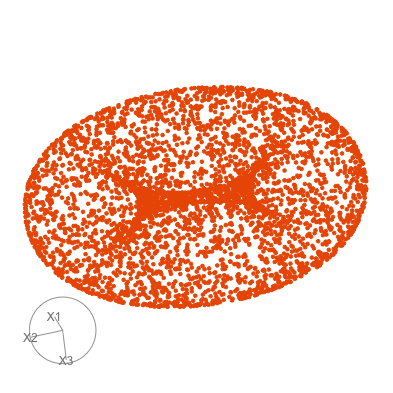
\includegraphics[keepaspectratio]{images/torus_proj.png}}

\subcaption{\label{}projection}
\end{minipage}%
%
\begin{minipage}{0.50\linewidth}

\pandocbounded{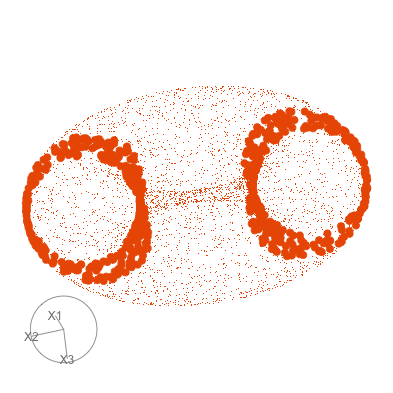
\includegraphics[keepaspectratio]{images/torus_slice.png}}

\subcaption{\label{}slice}
\end{minipage}%

\caption{\label{fig-slicing-pdf}Slicing can cut through high density is
useful to find hollowness in high-dimensional data, or understand
limitations of fitted models. Here points on the surface of a 3D torus
are shown using (a) projections, and (b) slices. The slicing reveals the
hollowness of this data with the circular cuts to the donut shape.
\faIcon{play-circle}}

\end{figure}%

It can also be useful to add layers to the data, such as summary
statistics, labels for selected observations, or connecting points with
lines to represent model fits. Figure~\ref{fig-adornments-pdf}
illustrates two use cases. In (a) labels for specific players are shown
when examining player statistics in the \texttt{aflw} data. All three
were named best players in the 2021 AFLW season, Bowers and Davey were
equal best and fairest, and Vescio was awarded best goal kicker. All
three have quite different player statistics profiles. The play of
Bowers and Davey differs in the number of handballs and kicks - Davey
tends to distribute the ball with handballs, while Bowers tends to kick.
In (b) the lines indicate constraints. This is compositional data where
each row adds to 1. It is the \texttt{Fireworks} data from the
\texttt{compositions} (van den Boogaart et al., 2024) package, and
measures the mixtures of five different ingredients. We can see that it
is relatively equal mixtures because all are very centred within the
constraints. We can also see points banding into stripes, suggesting
that there are just a small number of firework recipes.

\index{data!aflw} \index{data!fireworks}

\begin{figure}

\begin{minipage}{0.50\linewidth}

\pandocbounded{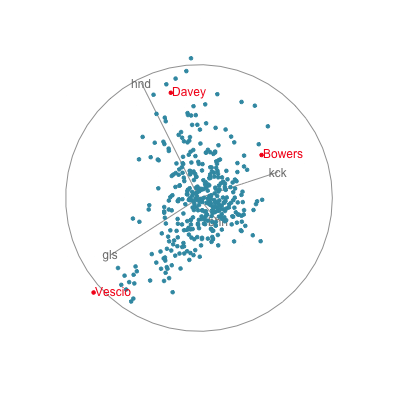
\includegraphics[keepaspectratio]{images/aflw_labelled.png}}

\subcaption{\label{}labelling}
\end{minipage}%
%
\begin{minipage}{0.50\linewidth}

\pandocbounded{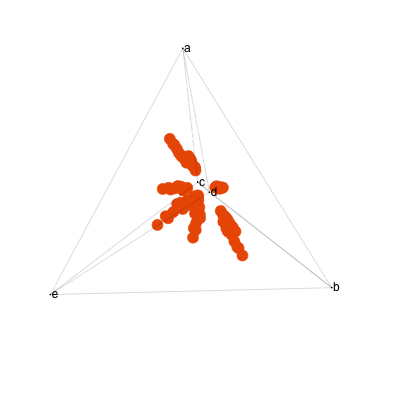
\includegraphics[keepaspectratio]{images/fireworks.png}}

\subcaption{\label{}constraints}
\end{minipage}%

\caption{\label{fig-adornments-pdf}It is sometimes useful to overlay
additional information, such as labels for a few points (a) or
representing constraints (b). The labels in (a) correspond to players
that won awards in the 2021 AFLW season. The lines in (b) correspond to
constraints - this is compositional data where each 5D observation is
constrained to sum to 1. \faIcon{play-circle}}

\end{figure}%

It is often asked why isn't the data display using solid shapes, or
provide depth cues with point size or colour. But the nature of
high-dimensions is that comprehensive research on lighting models and
perspective conducted for 3D graphics, does not extend to more than 3D.
For example, a light source, like a lamp, is a point object, and in 4D
the shadows would be 3D. A surface in 4D is 3D. So the choice of using
points to represent objects, and lines to indicate geometric features is
because these are meaningful in any dimension.

\section*{Exercises}\label{exercises-1}
\addcontentsline{toc}{section}{Exercises}

\markright{Exercises}

\begin{enumerate}
\def\labelenumi{\arabic{enumi}.}
\tightlist
\item
  Generate a matrix \(A\) with \(p=5\) (rows) and \(d=2\) (columns),
  where each value is randomly drawn from a standard normal
  distribution. Extract the element at row 3 and column 1.
\item
  We will interpret \(A\) as an orthonormal basis and therefore it needs
  to be checked for orthonormality, and if it fails, then to be
  orthonormalised. Use the function \texttt{tourr::is\_orthonormal} to
  explicitly check that each column is normalised and that the two
  columns are orthogonal. If they are not, then use
  \texttt{tourr::orthonormalise} to make them so. For the fixed version
  of \(A\), which dimensions contribute most to the projection,
  horizontally and vertically?
\item
  Use matrix multiplication to calculate the projection of the
  \texttt{mulgar::clusters} data onto the 2D plane defined by \(A\).
  Make a scatterplot of the projected data. Can you identify clustering
  in this view?
\item
  Use \texttt{save\_history()} to generate a grand tour path for the
  \texttt{mulgar::clusters} data, with three target planes. Extract and
  report the second target basis, and plot the resulting data.
\item
  Using the saved path, generate the interpolation between the target
  planes, using \texttt{interpolate()}. How many bases are in the tour
  path? Plot the first four in set of planes, and explain what is
  happening. Save tour path, extract basis and plot data
\item
  Repeat \texttt{save\_history()} but use a holes index guided tour.
  Plot the final projection. Does the guided tour find the three
  clusters? Which of the variables have the largest contributions to the
  differences between groups?
\item
  Repeat \texttt{save\_history()} using a radial tour, starting from the
  best projection basis from the guided tour, and exploring the
  contribution of \texttt{x1} (\texttt{mvar=1}). Why should the length
  of the path be set to three? Why is the last basis the same as the
  first? Examine the second target basis, and explain how it is
  different from the first basis.
\item
  Run the tours from in 4-7 using the \texttt{animate\_xy()}. You can
  use the \texttt{planned\_tour} method, but it is more interesting to
  simply re-generate using the different \texttt{tour\_path} methods. It
  is interesting to examine the importance of \texttt{x5} and
  \texttt{x4} to the clustering seen in the best projection from the
  guided tour.
\item
  Examine tours of 1D projections of the \texttt{mulgar::clusters} data,
  using density or histogram rendering. Can the three clusters be seen
  with 1D projections?
\item
  Explore the use of the slice tour on these geometric objects, that can
  be simulated using \texttt{geozoo}:
\end{enumerate}

\begin{enumerate}
\def\labelenumi{\alph{enumi}.}
\tightlist
\item
  Roman Surface, generated by
\end{enumerate}

\texttt{rs\ \textless{}-\ geozoo::roman.surface()\$points\ \textbar{}\textgreater{}\ scale()\ \textbar{}\textgreater{}\ as.data.frame()}

\begin{enumerate}
\def\labelenumi{\alph{enumi}.}
\setcounter{enumi}{1}
\tightlist
\item
  solid 4D sphere, generated by
\end{enumerate}

\texttt{s\_solid\ \textless{}-\ geozoo::sphere.solid.random(4,\ 2000)\$points\ \textbar{}\textgreater{}\ as.data.frame()}

\begin{enumerate}
\def\labelenumi{\alph{enumi}.}
\setcounter{enumi}{2}
\tightlist
\item
  hollow 4D sphere, generated by
\end{enumerate}

\texttt{s\_hollow\ \textless{}-\ geozoo::sphere.hollow(4,\ 2000)\$points\ \textbar{}\textgreater{}\ as.data.frame()}

Use both regular tours, and the slice tours on each. What does the slice
tour allow us to see in the Roman Surface? What is the difference
between the solid and hollow spheres?

\part{Dimension reduction}

\chapter{Dimension reduction overview}\label{sec-dimension-overview}

This chapter sets up the concepts related to methods for reducing
dimension such as principal component analysis (PCA) and t-stochastic
neighbour embedding (t-SNE), and how the tour can be used to assist with
these methods.

\section{The meaning of dimension}\label{the-meaning-of-dimension}

The number of variables, \(p\), is considered to be the dimension of the
data. However, the observed data may live in a lower dimensional
sub-space and then not fill out the full \(p\)-dimensions. This implicit
dimensionality is perceived in a tour using the spread of points. When
the points are spread far apart, then the data is filling the space.
Conversely, when the points ``collapse'' into a sub-region then the data
is only partially filling the space, and some dimension reduction to
reduce to this smaller dimensional space may be worthwhile.
\index{dimensionality!implicit}

\infobox{When exploring the implicit dimensionality of multivariate data we are looking for projections where the points do not fill the plotting canvas fully. This would indicate that the observed values do not fully populate high dimensions. }

Let's start with some 2D examples. Figure~\ref{fig-2D} shows three plots
of two variables. Plot (a) shows two variables that are strongly
linearly associated\footnote{It is generally better to use
  \emph{associated} than \emph{correlated}. Correlation is a statistical
  quantity, measuring linear association. The term \emph{associated} can
  be prefaced with the type of association, such as \emph{linear} or
  \emph{non-linear}.}, because when \texttt{x1} is low, \texttt{x2} is
low also, and conversely when \texttt{x1} is high, \texttt{x2} is also
high. This can also be seen by the reduction in spread of points (or
``collapse'') in one direction making the data fill less than the full
square of the plot. \emph{So from this we can conclude that the data is
not fully 2D.} The second step is to infer which variables contribute to
this reduction in dimension. The axes for \texttt{x1} and \texttt{x2}
are drawn extending from \((0,0)\) and because they both extend out of
the cloud of points, in the direction away from the collapse of points
we can say that they are jointly responsible for the dimension
reduction.

\infobox{The way variables are scaled can affect the appearance of dimensionity. If the variables are scaled together, using global values, some variables may have smaller variance than others. Scaling variables individually shifts the focus to association between variables, as the predominant reason for reduced dimension.}

Figure~\ref{fig-2D} (b) shows a pair of variables that are \textbf{not}
linearly associated. Variable \texttt{x1} is more varied than
\texttt{x3} but knowing the value on \texttt{x1} tells us nothing about
possible values on \texttt{x3}. Before running a tour all variables are
typically scaled to have equal spread. The purpose of the tour is to
capture association and relationships between the variables, so any
univariate differences should be removed ahead of time.
Figure~\ref{fig-2D} (c) shows what this would look like when \texttt{x3}
is scaled - the points are fully spread in the full square of the plot.

\begin{Shaded}
\begin{Highlighting}[]
\FunctionTok{library}\NormalTok{(tibble)}
\FunctionTok{set.seed}\NormalTok{(}\DecValTok{6045}\NormalTok{)}
\NormalTok{x1 }\OtherTok{\textless{}{-}} \FunctionTok{runif}\NormalTok{(}\DecValTok{123}\NormalTok{)}
\NormalTok{x2 }\OtherTok{\textless{}{-}}\NormalTok{ x1 }\SpecialCharTok{+} \FunctionTok{rnorm}\NormalTok{(}\DecValTok{123}\NormalTok{, }\AttributeTok{sd=}\FloatTok{0.1}\NormalTok{)}
\NormalTok{x3 }\OtherTok{\textless{}{-}} \FunctionTok{rnorm}\NormalTok{(}\DecValTok{123}\NormalTok{, }\AttributeTok{sd=}\FloatTok{0.2}\NormalTok{)}
\NormalTok{df }\OtherTok{\textless{}{-}} \FunctionTok{tibble}\NormalTok{(}\AttributeTok{x1 =}\NormalTok{ (x1}\SpecialCharTok{{-}}\FunctionTok{mean}\NormalTok{(x1))}\SpecialCharTok{/}\FunctionTok{sd}\NormalTok{(x1), }
             \AttributeTok{x2 =}\NormalTok{ (x2}\SpecialCharTok{{-}}\FunctionTok{mean}\NormalTok{(x2))}\SpecialCharTok{/}\FunctionTok{sd}\NormalTok{(x2),}
\NormalTok{             x3, }
             \AttributeTok{x3scaled =}\NormalTok{ (x3}\SpecialCharTok{{-}}\FunctionTok{mean}\NormalTok{(x3))}\SpecialCharTok{/}\FunctionTok{sd}\NormalTok{(x3))}
\end{Highlighting}
\end{Shaded}

\begin{figure}

\centering{

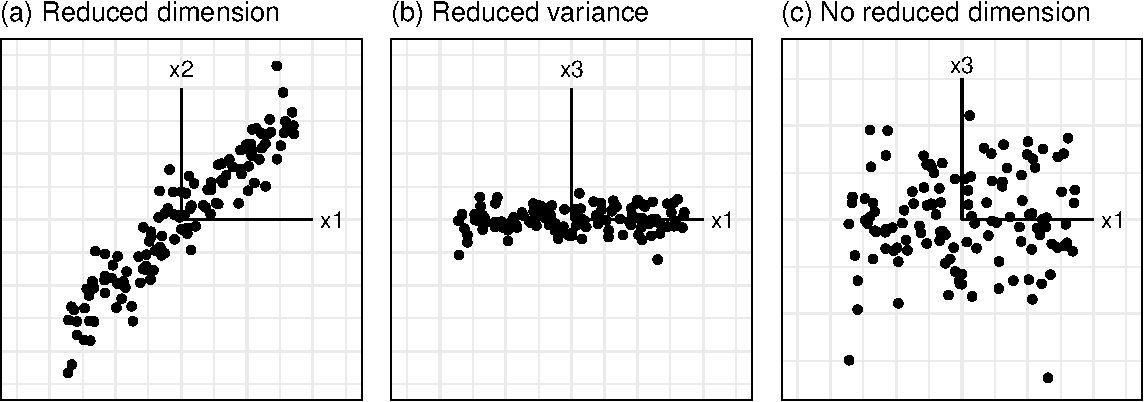
\includegraphics[width=1\linewidth,height=\textheight,keepaspectratio]{3-intro-dimred_files/figure-pdf/fig-2D-1.pdf}

}

\caption{\label{fig-2D}Explanation of how dimension reduction is
perceived in 2D, relative to variables: (a) Two variables with strong
linear association. Both variables contribute to the association, as
indicated by their axes extending out from the `collapsed' direction of
the points; (b) Two variables with no linear association. But x3 has
less variation, so points collapse in this direction; (c) The situation
in plot (b) does not arise in a tour because all variables are (usually)
scaled. When an axis extends out of a direction where the points are
collapsed, it means that this variable is partially responsible for the
reduced dimension.}

\end{figure}%

Figure~\ref{fig-nonlin-2D} illustrates other types of association that
could indicate reduced dimensionality. Plot (a) shows a strong nonlinear
association. Plots (b) and (c) show substantial regions of the data
space that have no observations, which may mean there is some barrier or
gap in the data generating process. The L-shape in plot (d) is a pattern
where one variable only shows variability if the other variable is
essentially all the same, say close to zero. It could be described as if
one variable has a non-zero value then the other variable is zero. This
is a very strong association pattern, but not one that is captured by
correlation. Plots (e) and (f) show other types of association, one with
heterogeneous variance depending on the subspace, and clustering of
observations, respectively. While we might detect these visually, using
dimension reduction methods with these structures can be tricky.

\begin{figure}

\centering{

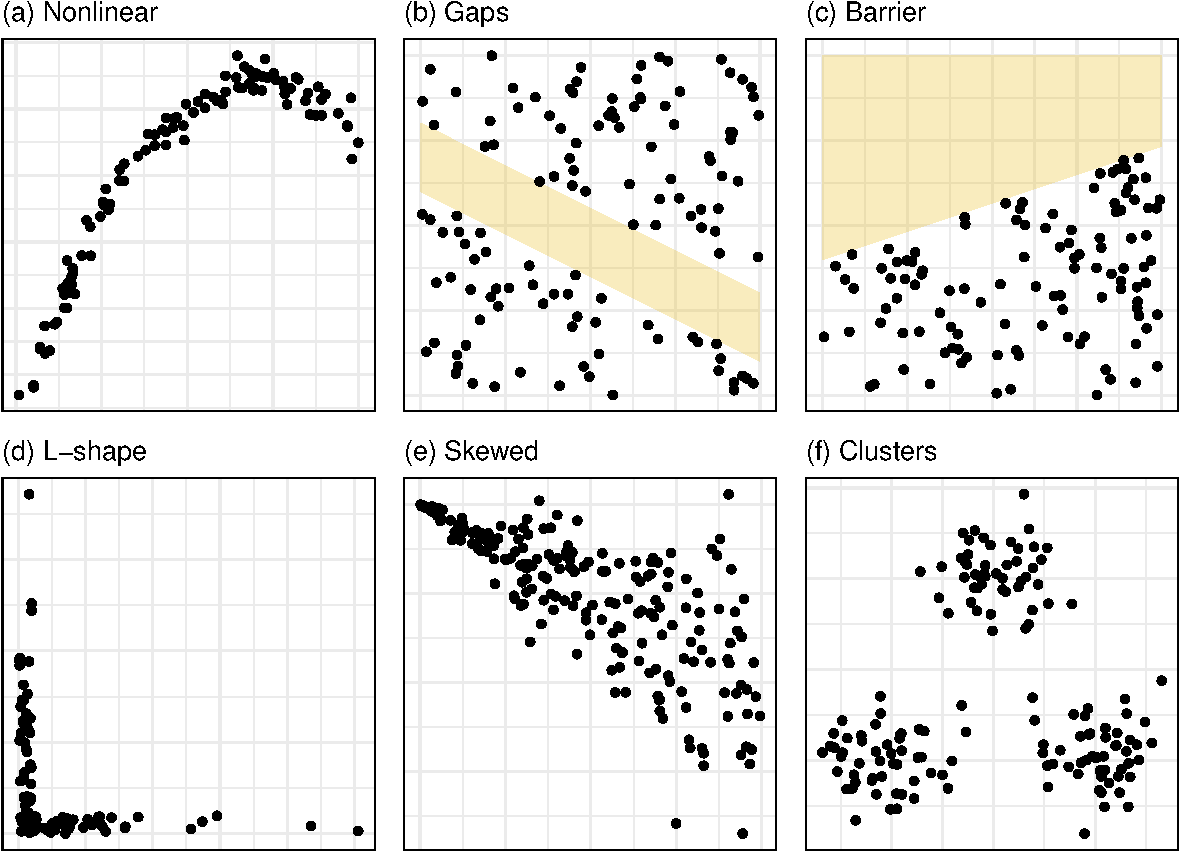
\includegraphics[width=1\linewidth,height=\textheight,keepaspectratio]{3-intro-dimred_files/figure-pdf/fig-nonlin-2D-1.pdf}

}

\caption{\label{fig-nonlin-2D}Other types of association: (a) nonlinear,
(b) gap between subspaces, (c) barrier beyond which no values are
observed, perhaps a limiting inequality constraint, (d) L-shape where is
one variable is observed the other is not, (e) skewness or heterogeneous
variance, (f) clustering.}

\end{figure}%

\section{How to perceive the dimensionality using a
tour}\label{how-to-perceive-the-dimensionality-using-a-tour}

Now let's think about what this looks like with five variables.
Figure~\ref{fig-dimension-pdf} shows a grand tour on five variables,
with (a) data that is primarily 2D, (b) data that is primarily 3D and
(c) fully 5D data. You can see that both (a) and (b) the spread of
points collapse in some projections, with it happening more in (a). In
(c) the data is always spread out in the square, although it does seem
to concentrate or pile in the centre. This piling is typical when
projecting from high dimensions to low dimensions. The sage tour (Laa et
al., 2022) makes a correction for this.

\begin{figure}

\begin{minipage}{0.33\linewidth}

\centering{

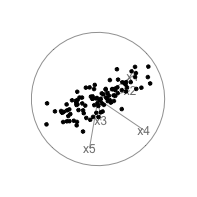
\includegraphics[width=1.66667in,height=\textheight,keepaspectratio]{images/plane.png}

}

\subcaption{\label{fig-plane}2D plane in 5D}

\end{minipage}%
%
\begin{minipage}{0.33\linewidth}

\centering{

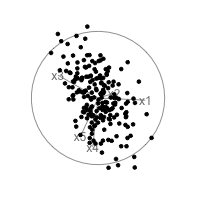
\includegraphics[width=1.66667in,height=\textheight,keepaspectratio]{images/box.png}

}

\subcaption{\label{fig-box}3D plane in 5D}

\end{minipage}%
%
\begin{minipage}{0.33\linewidth}

\centering{

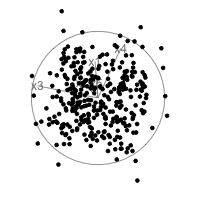
\includegraphics[width=1.66667in,height=\textheight,keepaspectratio]{images/cube5d.png}

}

\subcaption{\label{fig-cube5}5D plane in 5D}

\end{minipage}%

\caption{\label{fig-dimension-pdf}Single frames from different
dimensional planes - 2D, 3D, 5D - displayed in a grand tour projecting
into 2D. Notice that the 5D in 5D always fills out the box (although it
does concentrate some in the middle which is typical when projecting
from high to low dimensions). Also you can see that the 2D in 5D,
concentrates into a line more than the 3D in 5D. This suggests that it
is lower dimensional. \faIcon{play-circle}}

\end{figure}%

The next step is to determine which variables contribute. In the
examples just provided, all variables are linearly associated in the 2D
and 3D data. You can check this by making a scatterplot matrix,
Figure~\ref{fig-plane-scatmat}.

\begin{figure}

\centering{

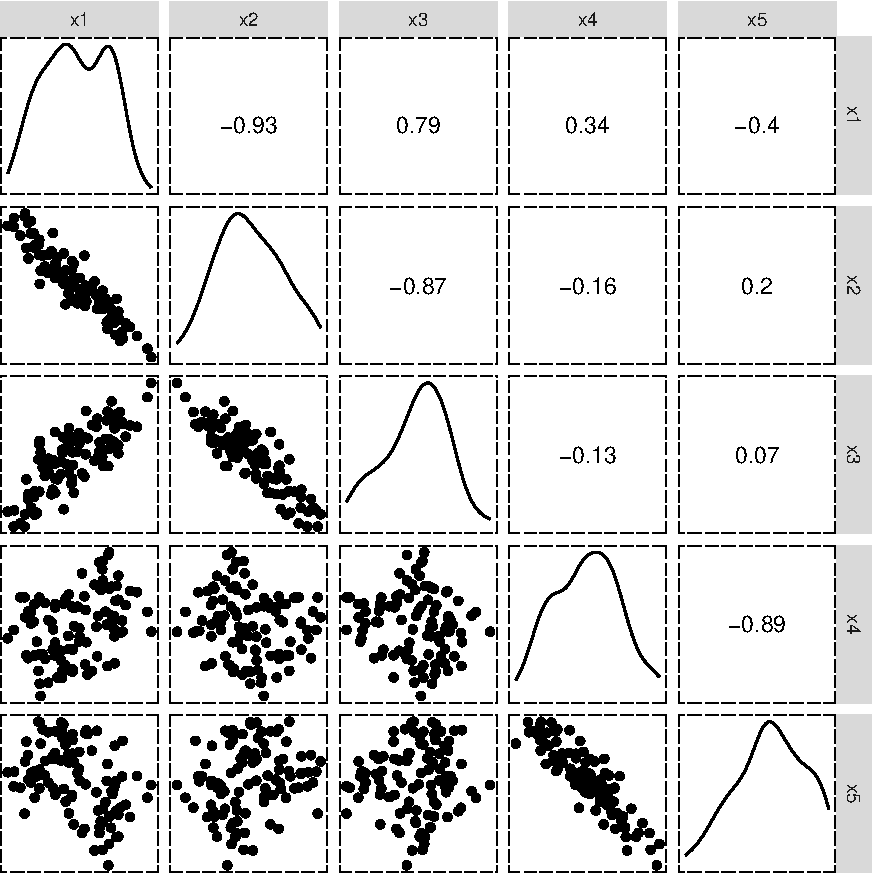
\includegraphics[width=0.8\linewidth,height=\textheight,keepaspectratio]{3-intro-dimred_files/figure-pdf/fig-plane-scatmat-1.pdf}

}

\caption{\label{fig-plane-scatmat}Scatterplot matrix of plane data. You
can see that x1-x3 are strongly linearly associated, and also x4 and x5.
When you watch the tour of this data, any time the data collapses into a
line you should see only (x1, x2, x3) or (x4, x5). When combinations of
x1 and x4 or x5 show, the data should be spread out.}

\end{figure}%

To make an example where not all variables contribute, we have added two
additional variables to the \texttt{plane} data set, which are purely
noise.

\begin{Shaded}
\begin{Highlighting}[]
\CommentTok{\# Add two pure noise dimensions to the plane}
\NormalTok{plane\_noise }\OtherTok{\textless{}{-}}\NormalTok{ plane}
\NormalTok{plane\_noise}\SpecialCharTok{$}\NormalTok{x6 }\OtherTok{\textless{}{-}} \FunctionTok{rnorm}\NormalTok{(}\DecValTok{100}\NormalTok{)}
\NormalTok{plane\_noise}\SpecialCharTok{$}\NormalTok{x7 }\OtherTok{\textless{}{-}} \FunctionTok{rnorm}\NormalTok{(}\DecValTok{100}\NormalTok{)}
\NormalTok{plane\_noise }\OtherTok{\textless{}{-}} \FunctionTok{data.frame}\NormalTok{(}\FunctionTok{apply}\NormalTok{(plane\_noise, }\DecValTok{2}\NormalTok{, }
    \ControlFlowTok{function}\NormalTok{(x) (x}\SpecialCharTok{{-}}\FunctionTok{mean}\NormalTok{(x))}\SpecialCharTok{/}\FunctionTok{sd}\NormalTok{(x)))}
\end{Highlighting}
\end{Shaded}

\begin{figure}

\centering{

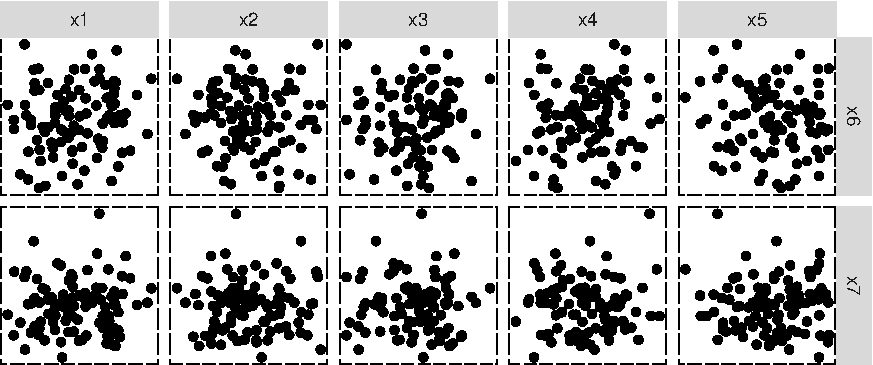
\includegraphics[width=0.8\linewidth,height=\textheight,keepaspectratio]{3-intro-dimred_files/figure-pdf/fig-plane-noise-scatter-1.pdf}

}

\caption{\label{fig-plane-noise-scatter}Scatterplots showing two
additional noise variables that are not associated with any of the first
five variables.}

\end{figure}%

Now we have 2D structure in 7D, but only five of the variables
contribute to the 2D structure, that is, five of the variables are
linearly related with each other. The other two variables (x6, x7) are
not linearly related to any of the others.

The data is viewed with a grand tour in
Figure~\ref{fig-plane-noise-pdf}. We can still see the concentration of
points along a line in some dimensions, which tells us that the data is
not fully 7D. Then if you look closely at the variable axes you will see
that the collapsing to a line only occurs when any of x1-x5 contribute
strongly in the direction orthogonal to this. This does not happen when
x6 or x7 contribute strongly to a projection - the data is always
expanded to fill much of the space. That tells us that x6 and x7 don't
substantially contribute to the dimension reduction, that is, they are
not linearly related to the other variables.

\begin{figure}

\begin{minipage}{0.50\linewidth}
\begin{center}
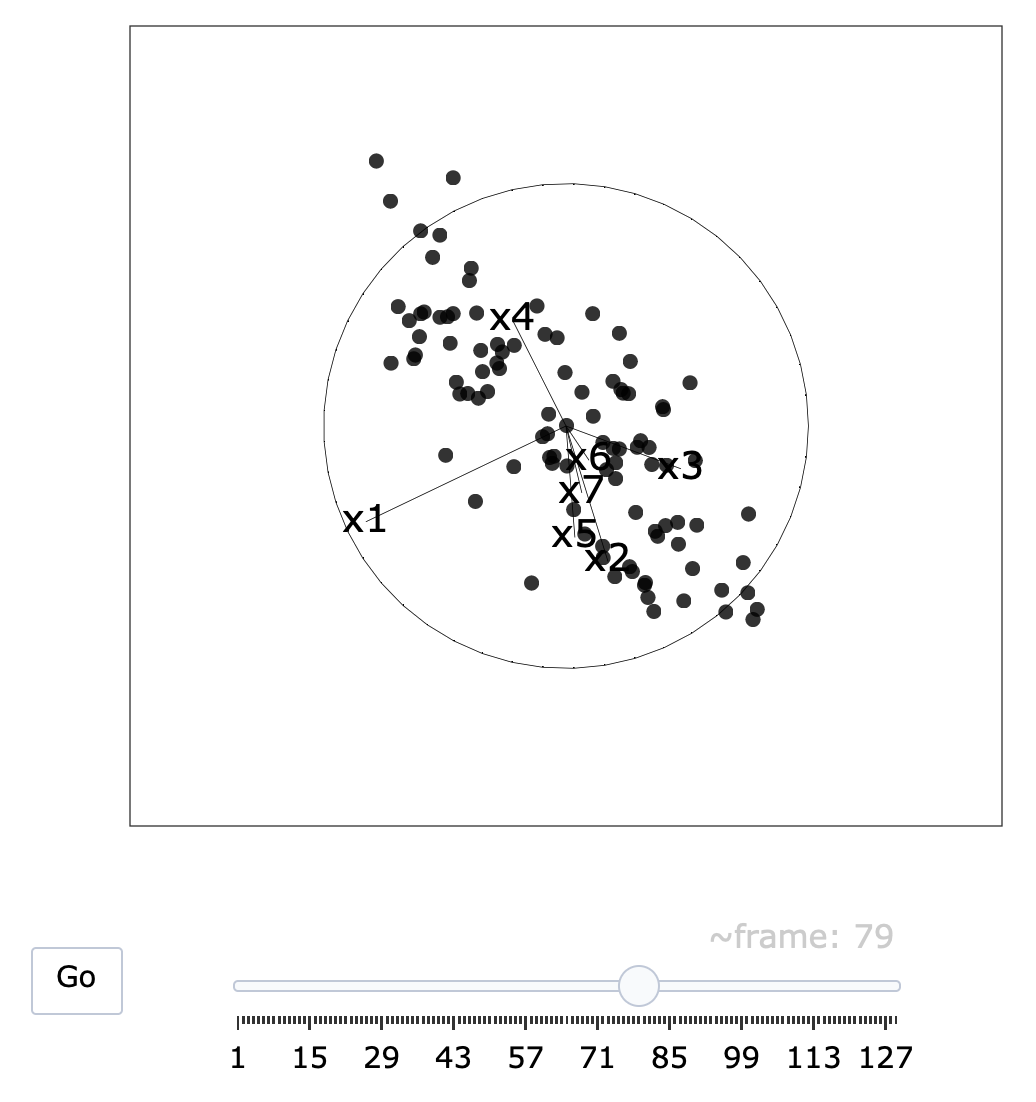
\includegraphics[width=2.08333in,height=\textheight,keepaspectratio]{images/plane_noise1.png}
\end{center}
\end{minipage}%
%
\begin{minipage}{0.50\linewidth}
\begin{center}
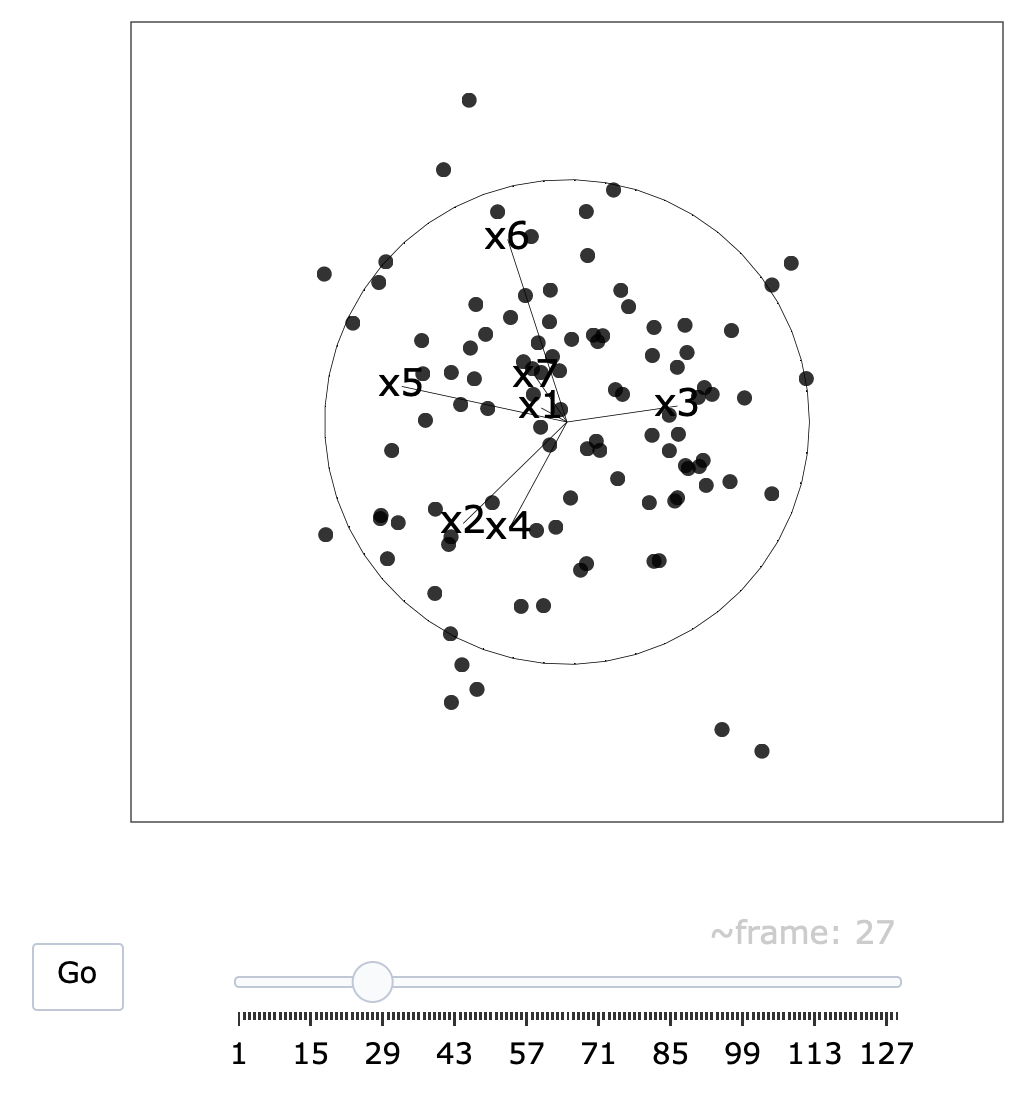
\includegraphics[width=2.08333in,height=\textheight,keepaspectratio]{images/plane_noise2.png}
\end{center}
\end{minipage}%

\caption{\label{fig-plane-noise-pdf}Two frames from a grand tour of the
plane with two additional dimensions of pure noise. The collapsing of
the points indicates that this is not fully 7D. This only happens when
any of x1-x5 are contributing strongly (frame 49 x4, x5; frame 79 x1;
frame 115 x2, x3). If x6 or x7 are contributing strongly the data is
spread out fully (frames 27, 96). This tells us that x6 and x7 are not
linearly associated, but other variables are. \faIcon{play-circle}}

\end{figure}%

\infobox{To determine which variables are responsible for the reduced dimension look for the axes that extend out of the point cloud. These contribute to smaller variation in the observations, and thus indicate possible dimension reduction using these variables}

The simulated data here is very simple, and what we have learned from
the tour could also be learned from principal component analysis.
However, if there are small complications, such as outliers or nonlinear
relationships, that might not be visible from principal component
analysis, the tour can help you to see them.

Figure~\ref{fig-plane-noise-outlier} and
Figure~\ref{fig-outlier-nonlin-pdf}(a) show example data with an outlier
and Figure~\ref{fig-outlier-nonlin-pdf}(b) shows data with non-linear
relationships.

\begin{Shaded}
\begin{Highlighting}[]
\CommentTok{\# Add several outliers to the plane\_noise data}
\NormalTok{plane\_noise\_outliers }\OtherTok{\textless{}{-}}\NormalTok{ plane\_noise}
\NormalTok{plane\_noise\_outliers[}\DecValTok{101}\NormalTok{,] }\OtherTok{\textless{}{-}} \FunctionTok{c}\NormalTok{(}\DecValTok{2}\NormalTok{, }\DecValTok{2}\NormalTok{, }\SpecialCharTok{{-}}\DecValTok{2}\NormalTok{, }\DecValTok{0}\NormalTok{, }\DecValTok{0}\NormalTok{, }\DecValTok{0}\NormalTok{, }\DecValTok{0}\NormalTok{)}
\NormalTok{plane\_noise\_outliers[}\DecValTok{102}\NormalTok{,] }\OtherTok{\textless{}{-}} \FunctionTok{c}\NormalTok{(}\DecValTok{0}\NormalTok{, }\DecValTok{0}\NormalTok{, }\DecValTok{0}\NormalTok{,}\SpecialCharTok{{-}}\DecValTok{2}\NormalTok{, }\SpecialCharTok{{-}}\DecValTok{2}\NormalTok{, }\DecValTok{0}\NormalTok{, }\DecValTok{0}\NormalTok{)}
\end{Highlighting}
\end{Shaded}

\begin{figure}

\centering{

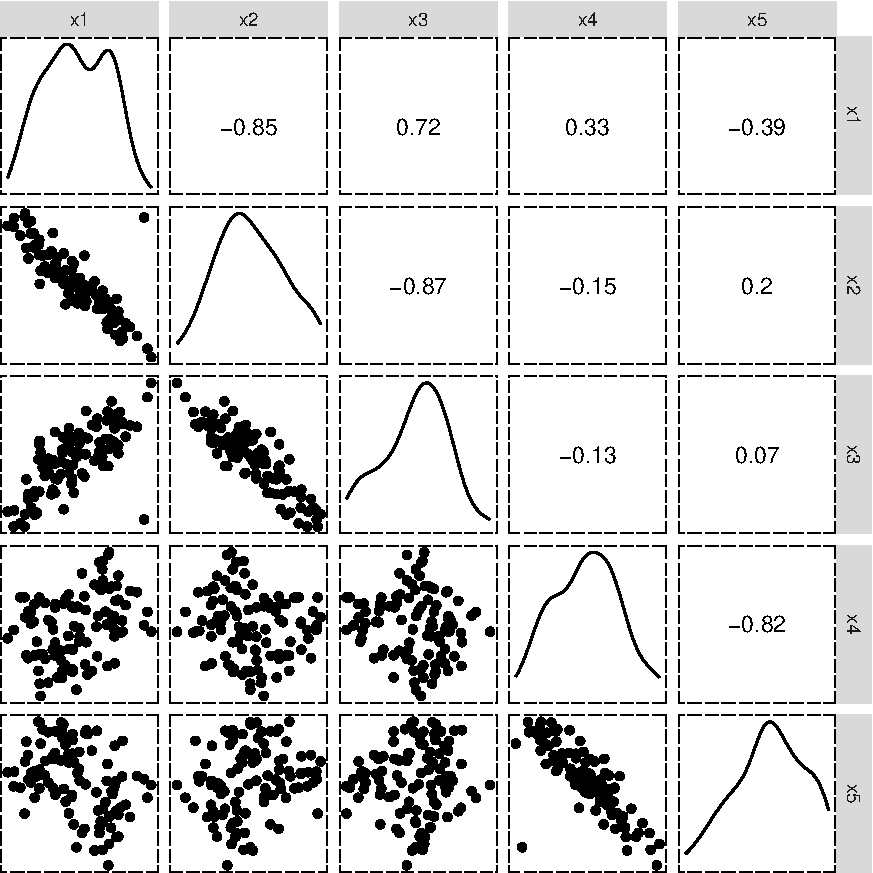
\includegraphics[width=0.8\linewidth,height=\textheight,keepaspectratio]{3-intro-dimred_files/figure-pdf/fig-plane-noise-outlier-1.pdf}

}

\caption{\label{fig-plane-noise-outlier}Scatterplot matrix of the plane
with noise data, with two added outliers in variables with strong
correlation.}

\end{figure}%

\begin{figure}

\begin{minipage}{0.50\linewidth}

\centering{

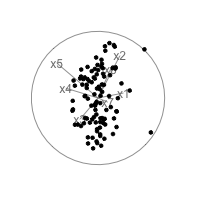
\includegraphics[width=2.08333in,height=\textheight,keepaspectratio]{images/pn_outliers.png}

}

\subcaption{\label{fig-outlier}Outliers}

\end{minipage}%
%
\begin{minipage}{0.50\linewidth}

\centering{

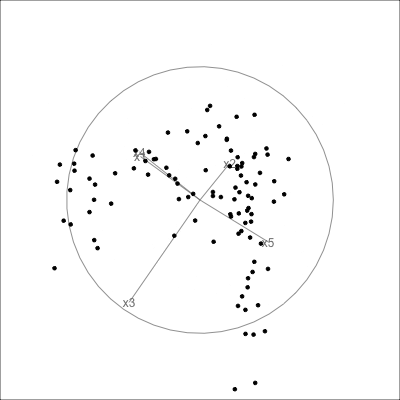
\includegraphics[width=2.08333in,height=\textheight,keepaspectratio]{images/plane_nonlin.png}

}

\subcaption{\label{fig-nonlinear}Non-linear relationship}

\end{minipage}%

\caption{\label{fig-outlier-nonlin-pdf}Two frames from tours of examples
of different types of dimensionality issues: outliers (a) and
non-linearity (b). In (a) you can see two points far from the others in
the projection. During a tour the two can be seen with different
movement patterns -- moving faster and in different directions than
other points. Outliers will affect detection of reduced dimension, but
they can be ignored when assessing dimensionality with the tour. In (b)
there is a non-linear relationship between several variables, primarily
with x3. Non-linear relationships may not be easily captured by other
techniques but are often visible with the tour. \faIcon{play-circle}}

\end{figure}%

\section*{Exercises}\label{exercises-2}
\addcontentsline{toc}{section}{Exercises}

\markright{Exercises}

\begin{enumerate}
\def\labelenumi{\arabic{enumi}.}
\tightlist
\item
  Multicollinearity is when the predictors for a model are strongly
  linearly associated. It can adversely affect the fitting of most
  models, because many possible models may be equally as good. Variable
  importance might be masked by correlated variables, and confidence
  intervals generated for linear models might be too wide. Check the for
  multicollinearity or other associations between the predictors in:

  \begin{enumerate}
  \def\labelenumii{\alph{enumii}.}
  \tightlist
  \item
    2001 Australian election data
  \item
    2016 Australian election data
  \end{enumerate}
\item
  Examine 5D multivariate normal samples drawn from populations with a
  range of variance-covariance matrices. (You can use the
  \texttt{mvtnorm} package to do the sampling, for example.) Examine the
  data using a grand tour. What changes when you change the correlation
  from close to zero to close to 1? Can you see a difference between
  strong positive correlation and strong negative correlation?
\item
  The following code shows how to hide a point in a four-dimensional
  space, so that it is not visible in any of the plots of two variables.
  Generate both \texttt{d} and \texttt{d\_r} and confirm that the point
  is visible in a scatterplot matrix of \texttt{d}, but not in the
  scatterplot matrix of \texttt{d\_r}. Also confirm that it is visible
  in both data sets when you use a tour.
\end{enumerate}

\begin{Shaded}
\begin{Highlighting}[]
\FunctionTok{library}\NormalTok{(tidyverse)}
\FunctionTok{library}\NormalTok{(tourr)}
\FunctionTok{library}\NormalTok{(GGally)}
\FunctionTok{set.seed}\NormalTok{(}\DecValTok{946}\NormalTok{)}
\NormalTok{d }\OtherTok{\textless{}{-}} \FunctionTok{tibble}\NormalTok{(}\AttributeTok{x1=}\FunctionTok{runif}\NormalTok{(}\DecValTok{200}\NormalTok{, }\SpecialCharTok{{-}}\DecValTok{1}\NormalTok{, }\DecValTok{1}\NormalTok{), }
            \AttributeTok{x2=}\FunctionTok{runif}\NormalTok{(}\DecValTok{200}\NormalTok{, }\SpecialCharTok{{-}}\DecValTok{1}\NormalTok{, }\DecValTok{1}\NormalTok{), }
            \AttributeTok{x3=}\FunctionTok{runif}\NormalTok{(}\DecValTok{200}\NormalTok{, }\SpecialCharTok{{-}}\DecValTok{1}\NormalTok{, }\DecValTok{1}\NormalTok{))}
\NormalTok{d }\OtherTok{\textless{}{-}}\NormalTok{ d }\SpecialCharTok{|\textgreater{}}
  \FunctionTok{mutate}\NormalTok{(}\AttributeTok{x4 =}\NormalTok{ x3 }\SpecialCharTok{+} \FunctionTok{runif}\NormalTok{(}\DecValTok{200}\NormalTok{, }\SpecialCharTok{{-}}\FloatTok{0.1}\NormalTok{, }\FloatTok{0.1}\NormalTok{))}
\CommentTok{\# outlier is visible in d}
\NormalTok{d }\OtherTok{\textless{}{-}} \FunctionTok{bind\_rows}\NormalTok{(d, }\FunctionTok{c}\NormalTok{(}\AttributeTok{x1=}\DecValTok{0}\NormalTok{, }\AttributeTok{x2=}\DecValTok{0}\NormalTok{, }\AttributeTok{x3=}\SpecialCharTok{{-}}\FloatTok{0.5}\NormalTok{, }\AttributeTok{x4=}\FloatTok{0.5}\NormalTok{))}

\CommentTok{\# Point is hiding in d\_r}
\NormalTok{d\_r }\OtherTok{\textless{}{-}}\NormalTok{ d }\SpecialCharTok{|\textgreater{}}
  \FunctionTok{mutate}\NormalTok{(}\AttributeTok{x1 =} \FunctionTok{cos}\NormalTok{(pi}\SpecialCharTok{/}\DecValTok{6}\NormalTok{)}\SpecialCharTok{*}\NormalTok{x1 }\SpecialCharTok{+} \FunctionTok{sin}\NormalTok{(pi}\SpecialCharTok{/}\DecValTok{6}\NormalTok{)}\SpecialCharTok{*}\NormalTok{x3,}
         \AttributeTok{x3 =} \SpecialCharTok{{-}}\FunctionTok{sin}\NormalTok{(pi}\SpecialCharTok{/}\DecValTok{6}\NormalTok{)}\SpecialCharTok{*}\NormalTok{x1 }\SpecialCharTok{+} \FunctionTok{cos}\NormalTok{(pi}\SpecialCharTok{/}\DecValTok{6}\NormalTok{)}\SpecialCharTok{*}\NormalTok{x3,}
         \AttributeTok{x2 =} \FunctionTok{cos}\NormalTok{(pi}\SpecialCharTok{/}\DecValTok{6}\NormalTok{)}\SpecialCharTok{*}\NormalTok{x2 }\SpecialCharTok{+} \FunctionTok{sin}\NormalTok{(pi}\SpecialCharTok{/}\DecValTok{6}\NormalTok{)}\SpecialCharTok{*}\NormalTok{x4,}
         \AttributeTok{x4 =} \SpecialCharTok{{-}}\FunctionTok{sin}\NormalTok{(pi}\SpecialCharTok{/}\DecValTok{6}\NormalTok{)}\SpecialCharTok{*}\NormalTok{x2 }\SpecialCharTok{+} \FunctionTok{cos}\NormalTok{(pi}\SpecialCharTok{/}\DecValTok{6}\NormalTok{)}\SpecialCharTok{*}\NormalTok{x4)}
\end{Highlighting}
\end{Shaded}

\begin{enumerate}
\def\labelenumi{\arabic{enumi}.}
\setcounter{enumi}{3}
\item
  Examine each of the challenge data sets \texttt{c1}, \texttt{c2},
  \ldots, \texttt{c7} from the the \texttt{mulgar} package for signs of
  the observed values not filling out the full \(p\) dimensions.
\item
  The data sets \texttt{assoc1}, \texttt{assoc2}, \texttt{assoc3} have
  other types of association. Can you detect what the associations are
  in each set?
\item
  The data sets \texttt{anomaly1}, \texttt{anomaly2}, \texttt{anomaly3},
  \texttt{anomaly4}, \texttt{anomaly5} all have single anomalies. For
  there to be an anomaly in a data set, there must be some association
  between the variables, and the anomaly doesn't conform to this
  association pattern. Can you find them?
\item
  XXX Use \texttt{covsim} package to simulate data
\end{enumerate}

\chapter{Principal component
analysis}\label{principal-component-analysis}

\index{dimension reduction!principal component analysis (PCA)}

Reducing dimensionality using principal component analysis (PCA) dates
back to Pearson (1901) and Hotelling (1933). The goal is to find a
smaller set of variables, \(q (< p)\), that contain as much information
as the original, as possible. The new set of variables, known as
principal components (PCs), are linear combinations of the original
variables. The PCs can be used to represent the data in a
lower-dimensional space. Jolliffe \& Cadima (2016) provides a
contemporary review of the century of developments in PCA.

The process is essentially an optimisation procedure, although PCA has
an analytical solution. It solves the problem of

\[
\max_{a_k} ~\text{Var} (Xa_k),
\] where \(X\) is the \(n \times p\) data matrix, \(a_k (k=1, ..., p)\)
is a 1D projection vector, called an eigenvector, and the
\(\text{Var} (Xa_k)\) is called an eigenvalue. PCA is a sequential
process: you first find the projection that captures the most variance,
then you find a projection that is orthogonal to the first axis that
captures the most variance in the \((p-1)\)-dimensional space, then you
find a projection that is orthogonal to the first two axes that captures
the most variance in the \((p-2)\)-dimensional space, and so on. The
eigenvectors define the combination of the original variables, and the
eigenvalues define the amount of total variance explained by each of the
new of variables. \index{dimension reduction!eigenvalue}
\index{dimension reduction!eigenvector}

\infobox{Visualisation can be used to assess if PCA is suitable to use to summarise the variation in the data. It is also used to detect other patterns -- clustering, outliers or non-linear association -- which are interesting to find and indicate that PCA is not suitable.}

PCA is very broadly useful for summarising linear association by using
combinations of the variables that are highly correlated. However, high
correlation can also occur when there are outliers, or clustering. PCA
is commonly used to detect these patterns also, although this might NOT
be a reliable way to do so. To detect clustering or anomalies, using
more a different approach that is specifically focused on these types of
patterns is advisable. To some extent capturing clustering or anomalies
using PCA is actually finding problematic patterns that adversely
affects conducting appropriate dimension reduction.

PCA is not very effective when the distribution of the variables is
highly skewed, so it can be helpful to transform variables to make them
more symmetrically distributed before conducting PCA. It is also
possible to summarise different types of structure by generalising the
optimisation criteria to any function of projected data, \(f(XA)\),
which is called \emph{projection pursuit} (PP). PP has a long history
(Kruskal (1964a), Friedman \& Tukey (1974), Diaconis \& Freedman
(1984b), Jones \& Sibson (1987), Huber (1985)), and there are regularly
new developments (e.g. E.-K. Lee \& Cook (2009), Perisic \& Posse
(2005), Y. D. Lee et al. (2013), Loperfido (2018), Bickel et al. (2018),
C. Zhang et al. (2023)).

\section{Determining how many
dimensions}\label{determining-how-many-dimensions}

We would start by examining the data using a grand tour. The goal is to
check whether there might be potential issues for PCA, such as skewness,
outliers or clustering, or even non-linear dependencies.

We'll start by showing PCA on the simulated data from
Chapter~\ref{sec-dimension-overview}. The scree plots are produced using
the \texttt{mulgar::ggscree()} function, and include a grey guideline to
help decide how many PCs are sufficient. This guideline is generated by
taking the median value from of the eigenvalues generated by doing PCA
on 100 samples from a standard multivariate normal distribution. Any
values much lower than this line would indicate that those PCs are not
contributing to the explanation of variation. For these three simulated
examples, the scree plots illustrate that PCA supports that the data are
2D, 3D and 5D respectively.

\index{dimension reduction!scree plot}

\begin{figure}

\centering{

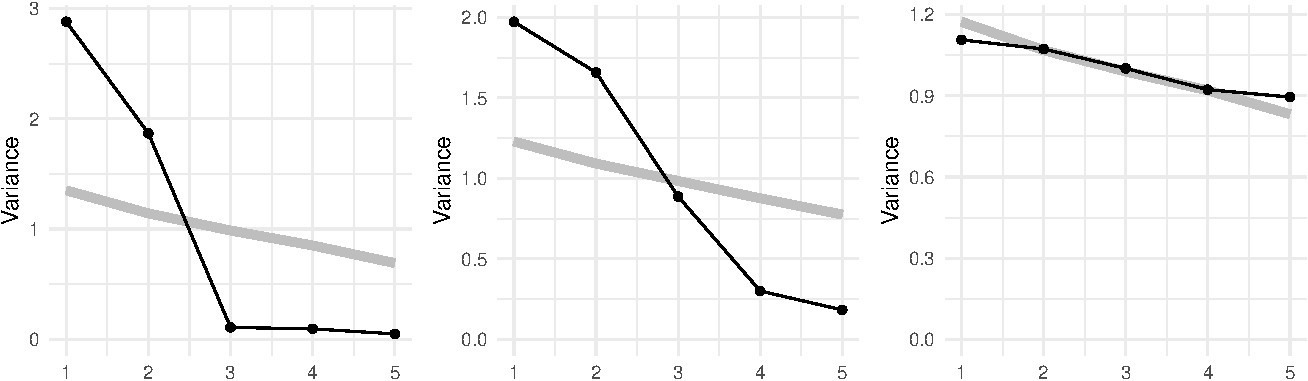
\includegraphics[width=1\linewidth,height=\textheight,keepaspectratio]{4-pca_files/figure-pdf/fig-2D-pca-1.pdf}

}

\caption{\label{fig-2D-pca}Scree plots for the three simulated data sets
shown in Figure 3.2. The 2D in 5D is clearly recognised by PCA to be 2D
because the variance drops substantially between 2-3 principal
components. The 3D in 5D is possibly 3D because the variance drops from
3-4 principal components. The fully 5D data has no drop in variance, and
all values are close to the typical value one would observe if the data
was fully 5D.}

\end{figure}%

The next step is to look at the coefficients for the selected number of
PCs. Table~\ref{tbl-plane-pcs} shows the coefficients for the first two
PCs of the \texttt{plane} data. All five variables contribute, with
\texttt{x1}, \texttt{x2}, \texttt{x3} contributing more to \texttt{PC1},
and \texttt{x4}, \texttt{x5} contributing more to \texttt{PC2}.
Table~\ref{tbl-box-pcs} shows the coefficients for the first three PCs
of the \texttt{box} data. Variables \texttt{x1}, \texttt{x2},
\texttt{x3} contribute strongly to \texttt{PC1}, \texttt{PC2} has
contributions from all variables except \texttt{x3} and variables
\texttt{x4} and \texttt{x5} contribute strongly to \texttt{PC3}.

\index{dimension reduction!coefficients}
\index{dimension reduction!principal components}

\begin{longtable}{lrr}

\caption{\label{tbl-plane-pcs}Coefficients for the first two PCs for the
plane data.}

\tabularnewline

\toprule
Variable & PC1 & PC2 \\ 
\midrule\addlinespace[2.5pt]
x1 & $0.58$ & $-0.06$ \\ 
x2 & $-0.55$ & $0.21$ \\ 
x3 & $0.47$ & $-0.41$ \\ 
x4 & $0.25$ & $0.64$ \\ 
x5 & $-0.29$ & $-0.62$ \\ 
\bottomrule

\end{longtable}

\begin{longtable}{lrrr}

\caption{\label{tbl-box-pcs}Coefficients for the first three PCs for the
box data.}

\tabularnewline

\toprule
Variable & PC1 & PC2 & PC3 \\ 
\midrule\addlinespace[2.5pt]
x1 & $-0.51$ & $0.46$ & $0.11$ \\ 
x2 & $0.51$ & $0.46$ & $0.00$ \\ 
x3 & $-0.65$ & $-0.09$ & $0.23$ \\ 
x4 & $-0.22$ & $0.36$ & $-0.87$ \\ 
x5 & $0.02$ & $0.66$ & $0.43$ \\ 
\bottomrule

\end{longtable}

In each of these simulated data sets, all five variables contributed to
the dimension reduction. If we added two purely noise variables to the
plane data, as done in Chapter~\ref{sec-dimension-overview}, the scree
plot in Figure~\ref{fig-plane-noise-scree} would indicate that the data
is now 4D, and we would get a different interpretation of the
coefficients from the PCA, see Table~\ref{tbl-plane-noise-pcs}. We see
that \texttt{PC1} and \texttt{PC2} are approximately the same as before,
with main variables being (\texttt{x1}, \texttt{x2}, \texttt{x3}) and
(\texttt{x4}, \texttt{x5}) respectively. \texttt{PC3} and \texttt{PC4}
are both \texttt{x6} and \texttt{x7}.

\begin{figure}

\centering{

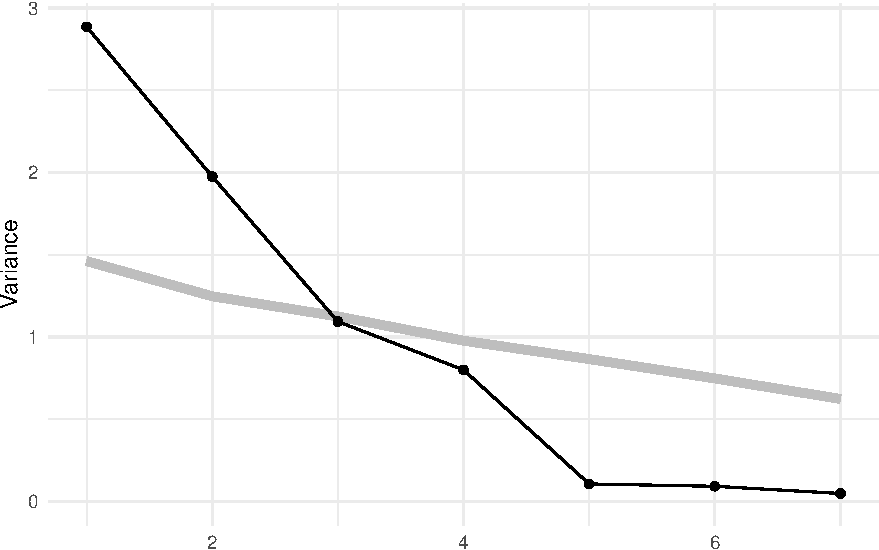
\includegraphics[width=0.8\linewidth,height=\textheight,keepaspectratio]{4-pca_files/figure-pdf/fig-plane-noise-scree-1.pdf}

}

\caption{\label{fig-plane-noise-scree}Additional noise variables expands
the plane data to 4D.}

\end{figure}%

\begin{longtable}{lrrrr}

\caption{\label{tbl-plane-noise-pcs}Coefficients for PCs 1-4 of the
plane plus noise data.}

\tabularnewline

\toprule
Variable & PC1 & PC2 & PC3 & PC4 \\ 
\midrule\addlinespace[2.5pt]
x1 & $0.58$ & $0.04$ & $0.01$ & $0.00$ \\ 
x2 & $-0.55$ & $-0.18$ & $-0.03$ & $0.07$ \\ 
x3 & $0.47$ & $0.37$ & $0.05$ & $-0.20$ \\ 
x4 & $0.24$ & $-0.62$ & $-0.06$ & $0.17$ \\ 
x5 & $-0.28$ & $0.60$ & $0.07$ & $-0.14$ \\ 
x6 & $0.05$ & $0.29$ & $-0.58$ & $0.76$ \\ 
x7 & $-0.02$ & $-0.08$ & $-0.81$ & $-0.58$ \\ 
\bottomrule

\end{longtable}

\subsection{Example: pisa}\label{example-pisa}

\index{data!pisa}

The \texttt{pisa} data contains simulated data from math, reading and
science scores, totalling 30 variables. PCA is used here to examine the
association. We might expect that it is 3D, but what we see suggests it
is primarily 1D. This means that a student that scores well in math,
will also score well in reading and science.

\begin{Shaded}
\begin{Highlighting}[]
\FunctionTok{data}\NormalTok{(pisa)}
\NormalTok{pisa\_std }\OtherTok{\textless{}{-}}\NormalTok{ pisa }\SpecialCharTok{|\textgreater{}}
  \FunctionTok{filter}\NormalTok{(CNT }\SpecialCharTok{==} \StringTok{"Australia"}\NormalTok{) }\SpecialCharTok{|\textgreater{}}
  \FunctionTok{select}\NormalTok{(}\SpecialCharTok{{-}}\NormalTok{CNT) }\SpecialCharTok{|\textgreater{}}
  \FunctionTok{mutate\_all}\NormalTok{(mulgar}\SpecialCharTok{:::}\NormalTok{scale2)}
\NormalTok{pisa\_pca }\OtherTok{\textless{}{-}} \FunctionTok{prcomp}\NormalTok{(pisa\_std)}
\NormalTok{pisa\_scree }\OtherTok{\textless{}{-}} \FunctionTok{ggscree}\NormalTok{(pisa\_pca, }\AttributeTok{q =} \DecValTok{15}\NormalTok{) }\SpecialCharTok{+} \FunctionTok{theme\_minimal}\NormalTok{()}
\end{Highlighting}
\end{Shaded}

The scree plot in Figure~\ref{fig-pisa-pca-pdf} shows a big drop from
one to two PCs in the amount of variance explained. From a grand tour on
the 30 variables we can see that the data is elliptical in most
projections, sometimes shrinking to be a small circle. This pattern
strongly indicates that there is one primary direction of variation in
the data, with only small variation in any direction away from it.
Shrinking to the small circle is analogous to to how \emph{a pencil or
cigar or water bottle in 3D looks from some angles}.

\begin{figure}

\begin{minipage}{0.50\linewidth}

\centering{

\pandocbounded{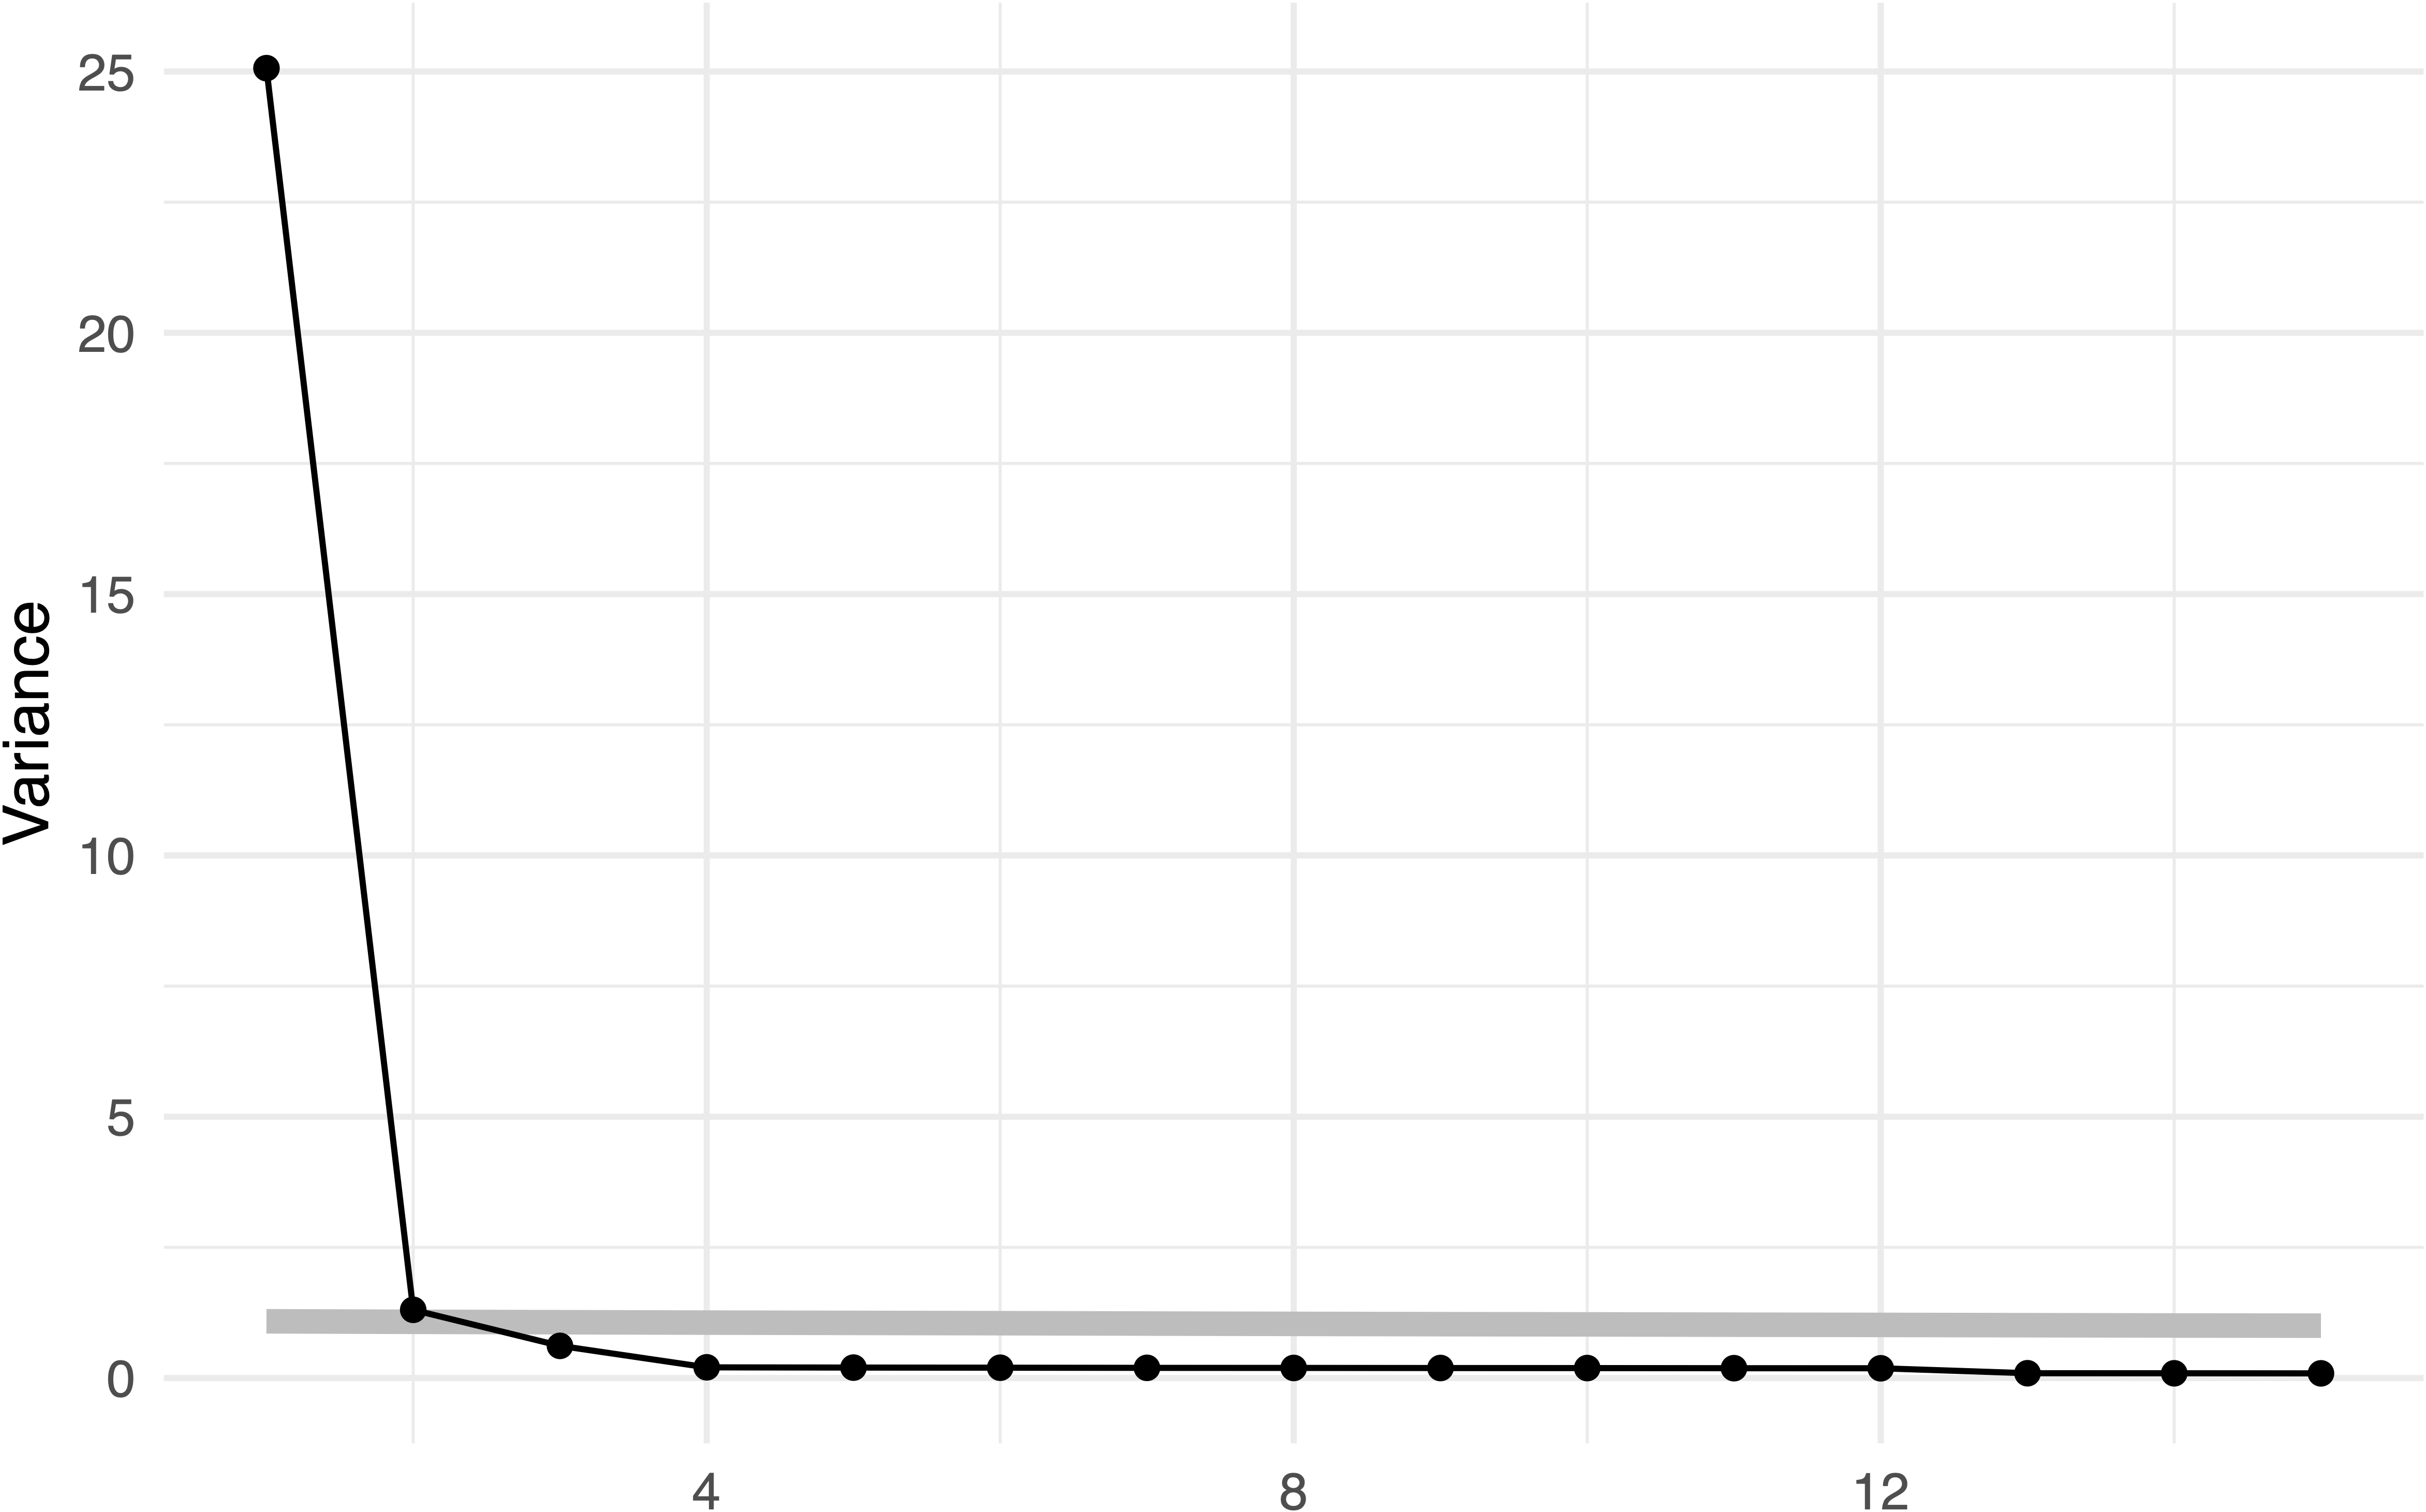
\includegraphics[keepaspectratio]{images/fig-pisa-scree-1.png}}

}

\subcaption{\label{fig-pisa-scree-pdf}Scree plot}

\end{minipage}%
%
\begin{minipage}{0.50\linewidth}

\centering{

\pandocbounded{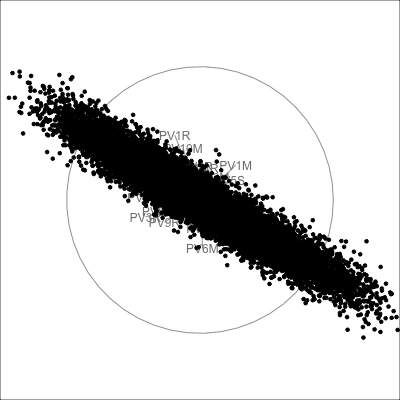
\includegraphics[keepaspectratio]{images/pisa_gt_249.png}}

}

\subcaption{\label{fig-pisa-gt}Grand tour frame}

\end{minipage}%

\caption{\label{fig-pisa-pca-pdf}Scree plot and a frame from a tour of
the \texttt{pisa} data, with 30 variables being the plausible scores for
Australian students. In combination, these suggest that the data is
effectively 1D. \faIcon{play-circle}}

\end{figure}%

The coefficients of the first PC (first eigenvector) are roughly equal
in magnitude (as shown below), which tells us that all variables roughly
contribute. Interestingly, they are all negative, which is not actually
meaningful. With different software these could easily have been all
positive. The sign of the coefficients can be reversed, as long as all
are reversed, which is the same as an arrow pointing one way, changing
and pointing the other way.

\begin{Shaded}
\begin{Highlighting}[]
\FunctionTok{round}\NormalTok{(pisa\_pca}\SpecialCharTok{$}\NormalTok{rotation[,}\DecValTok{1}\NormalTok{], }\DecValTok{2}\NormalTok{)}
\end{Highlighting}
\end{Shaded}

\begin{verbatim}
 PV1MATH  PV2MATH  PV3MATH  PV4MATH  PV5MATH  PV6MATH 
   -0.18    -0.18    -0.18    -0.18    -0.18    -0.18 
 PV7MATH  PV8MATH  PV9MATH PV10MATH  PV1READ  PV2READ 
   -0.18    -0.18    -0.18    -0.18    -0.19    -0.18 
 PV3READ  PV4READ  PV5READ  PV6READ  PV7READ  PV8READ 
   -0.19    -0.19    -0.19    -0.19    -0.19    -0.19 
 PV9READ PV10READ  PV1SCIE  PV2SCIE  PV3SCIE  PV4SCIE 
   -0.19    -0.19    -0.18    -0.18    -0.19    -0.18 
 PV5SCIE  PV6SCIE  PV7SCIE  PV8SCIE  PV9SCIE PV10SCIE 
   -0.19    -0.18    -0.19    -0.18    -0.19    -0.18 
\end{verbatim}

\insightbox{The tour verifies that the `pisa` data is primarily 1D, indicating that a student who scores well in math, probably scores well in reading and science, too. More interestingly, the regular shape of the data strongly indicates that it is "synthetic", simulated rather than observed.}

\subsection{Example: aflw}\label{example-aflw}

\index{data!aflw}

This data has player statistics for all the matches in the 2021 season.
We would be interested to know which variables contain similar
information, and thus might be combined into single variables. We would
expect that many statistics group into a few small sets, such as
offensive and defensive skills. We might also expect that some of the
statistics are skewed, most players have low values and just a handful
of players are stellar. It is also possible that there are some extreme
values. These are interesting features, but they will distract from the
main purpose of grouping the statistics. Thus the tour is used to check
for potential problems with the data prior to conducting PCA.

\begin{Shaded}
\begin{Highlighting}[]
\FunctionTok{library}\NormalTok{(tourr)}
\FunctionTok{data}\NormalTok{(aflw)}
\NormalTok{aflw\_std }\OtherTok{\textless{}{-}}\NormalTok{ aflw }\SpecialCharTok{|\textgreater{}}
  \FunctionTok{mutate\_if}\NormalTok{(is.numeric, }\ControlFlowTok{function}\NormalTok{(x) (x}\SpecialCharTok{{-}}
      \FunctionTok{mean}\NormalTok{(x, }\AttributeTok{na.rm=}\ConstantTok{TRUE}\NormalTok{))}\SpecialCharTok{/}
      \FunctionTok{sd}\NormalTok{(x, }\AttributeTok{na.rm=}\ConstantTok{TRUE}\NormalTok{))}
\end{Highlighting}
\end{Shaded}

To look at all of the 29 player statistics in a grand tour in
Figure~\ref{fig-aflw-gt-pdf}.

\begin{figure}

\begin{minipage}{0.50\linewidth}
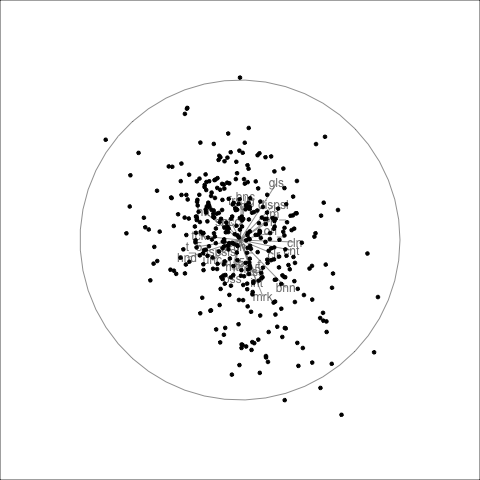
\includegraphics[width=2.375in,height=\textheight,keepaspectratio]{images/aflw_gt_70.png}\end{minipage}%
%
\begin{minipage}{0.50\linewidth}
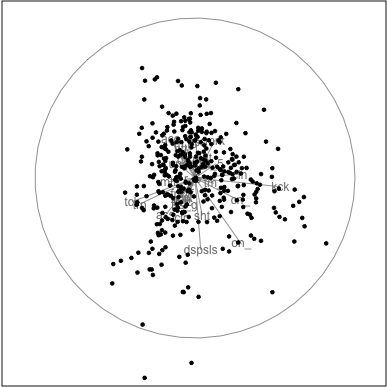
\includegraphics[width=2.375in,height=\textheight,keepaspectratio]{images/aflw_gt_329.png}\end{minipage}%

\caption{\label{fig-aflw-gt-pdf}Two frames from a grand tour of the AFLW
player statistics. Most player statistics concentrate near the centre,
indicating most players are ``average''! There are a few outliers
appearing in different combinations of the skills, which one would
expect to be the star players for particular skill sets.
\faIcon{play-circle}}

\end{figure}%

No major surprises! There is a small amount of skewness, and there are
no major outliers. Skewness indicates that most players have reasonably
similar skills (bunching of points), except for some key players (the
moderate outliers). The skewness could be reduced by applying a log or
square root transformation to some variables prior to running the PCA.
However, we elect not to do this because the moderate outliers are of
interest. These correspond to talented players that we'd like to explore
further with the analysis.

Below we have the conventional summary of the PCA, a scree plot showing
the reduction in variance to be explained when each additional PC is
considered. It is also conventional to look at a table summarising the
proportions of variance explained by PCs, but with almost 30 variables
it is easier to make some decision on the number of PCs needed based on
the scree plot.

\begin{figure}

\centering{

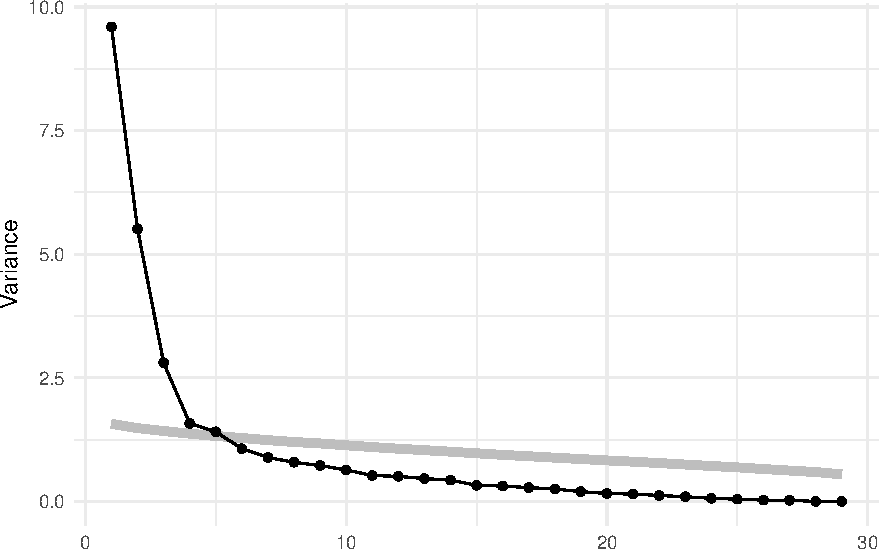
\includegraphics[width=0.8\linewidth,height=\textheight,keepaspectratio]{4-pca_files/figure-pdf/fig-aflw-pca-1.pdf}

}

\caption{\label{fig-aflw-pca}Scree plot showing decay in variance of
PCs. There are sharp drops for the first four PCs, and then smaller
declines.}

\end{figure}%

\index{dimension reduction!scree plot}

From the scree plot in Figure~\ref{fig-aflw-pca}, we see a sharp drop
from one to two, two to three and then smaller drops. After four PCs the
variance drops again at six PCs and then gradually decays. We will
choose four PCs to examine more closely. This explains 67.2\% of the
variance.

\begin{longtable}{lrrrr}

\caption{\label{tbl-aflw-pcs}Coefficients for the first four PCs. PC 1
contrasts some with PC 1, with the first having large coefficients
primarily on field play statistics, and the second having large
coefficients on the scoring statistics.}

\tabularnewline

\toprule
Variable & PC1 & PC2 & PC3 & PC4 \\ 
\midrule\addlinespace[2.5pt]
disposals & $0.31$ & $-0.05$ & $-0.03$ & $0.07$ \\ 
possessions & $0.31$ & $-0.03$ & $-0.07$ & $0.09$ \\ 
kicks & $0.29$ & $-0.04$ & $0.09$ & $-0.12$ \\ 
metres & $0.28$ & $-0.03$ & $0.10$ & $-0.15$ \\ 
contested & $0.28$ & $0.01$ & $-0.12$ & $0.23$ \\ 
uncontested & $0.28$ & $-0.06$ & $-0.01$ & $-0.05$ \\ 
turnovers & $0.27$ & $-0.01$ & $-0.01$ & $-0.29$ \\ 
clearances & $0.23$ & $0.00$ & $-0.29$ & $0.19$ \\ 
clangers & $0.23$ & $-0.02$ & $-0.06$ & $-0.33$ \\ 
handballs & $0.23$ & $-0.04$ & $-0.19$ & $0.31$ \\ 
frees\_for & $0.21$ & $0.02$ & $-0.13$ & $0.18$ \\ 
marks & $0.21$ & $0.03$ & $0.32$ & $0.02$ \\ 
tackles & $0.20$ & $0.01$ & $-0.28$ & $0.09$ \\ 
time\_pct & $0.16$ & $-0.04$ & $0.35$ & $-0.02$ \\ 
intercepts & $0.13$ & $-0.28$ & $0.24$ & $0.03$ \\ 
rebounds\_in50 & $0.13$ & $-0.28$ & $0.24$ & $-0.06$ \\ 
frees\_against & $0.13$ & $0.03$ & $-0.16$ & $-0.23$ \\ 
assists & $0.09$ & $0.23$ & $0.00$ & $0.05$ \\ 
bounces & $0.09$ & $0.03$ & $0.02$ & $-0.28$ \\ 
behinds & $0.09$ & $0.32$ & $0.08$ & $-0.02$ \\ 
shots & $0.08$ & $0.38$ & $0.12$ & $-0.03$ \\ 
tackles\_in50 & $0.07$ & $0.27$ & $-0.18$ & $0.03$ \\ 
marks\_in50 & $0.06$ & $0.34$ & $0.18$ & $0.04$ \\ 
contested\_marks & $0.05$ & $0.16$ & $0.34$ & $0.15$ \\ 
goals & $0.04$ & $0.37$ & $0.16$ & $0.03$ \\ 
accuracy & $0.04$ & $0.34$ & $0.10$ & $0.06$ \\ 
one\_pct & $0.03$ & $-0.21$ & $0.33$ & $0.08$ \\ 
disposal & $0.02$ & $-0.13$ & $0.20$ & $0.50$ \\ 
hitouts & $-0.04$ & $0.00$ & $-0.03$ & $0.32$ \\ 
\bottomrule

\end{longtable}

When there are as many variables as this, it can be hard to digest the
combinations of variables most contributing to each PC. Rearranging the
table by sorting on a selected PC can help. Table~\ref{tbl-aflw-pcs} has
been sorted according to the PC 1 coefficients.

PC 1 is primarily composed of \texttt{disposals}, \texttt{possessions},
\texttt{kicks}, \texttt{metres}, \texttt{uncontested},
\texttt{contested}, \ldots. primarily the field play statistics! It is
quite common in PCA for the first PC to be a combination of all
variables, which suggests that there is one main direction of variation
in the data. Here it is not quite that. PCA suggests that the primary
variation is through a combination of field skills, or basic football
playing skills.

Thus the second PC contrasts the first, because it is primarily a
combination of \texttt{shots}, \texttt{goals}, \texttt{marks\_in50},
\texttt{accuracy}, and \texttt{behinds} contrasted against
\texttt{rebounds\_in50} and \texttt{intercepts}. The positive
coefficients are primary offensive skills and the negative coefficients
are defensive skills. This PC is reasonable measure of the offensive vs
defensive skills of a player.

\index{dimension reduction!interpretation}

We could continue to interpret each PC by examining large coefficients
to help decide how many PCs are a suitable summary of the information in
the data. Briefly, PC 3 mixed but it is possibly a measure of worth of
the player because \texttt{time\_pct} has a large coefficient, so
players that are on the field longer will contribute strongly to this
new variable. It also has large (and opposite) contributions from
\texttt{clearances}, \texttt{tackles}, \texttt{contested\_marks}. PC 4
appears to be related to aggressive play with \texttt{clangers},
\texttt{turnovers}, \texttt{bounces} and \texttt{frees\_against}
featuring. All four PCs have useful information.

For deeper exploration, when we tour the four PCs, we'd like to be able
to stop and identify players. This can be done by creating a
pre-computed animation, with additional mouse-over, made using
\texttt{plotly}. However, it is not size-efficient, can is only feasible
with a small number of observations. Because all of the animation frames
with the fully projected data in each, are composed into a single
object, which gets large very quickly.

\begin{figure}

\centering{

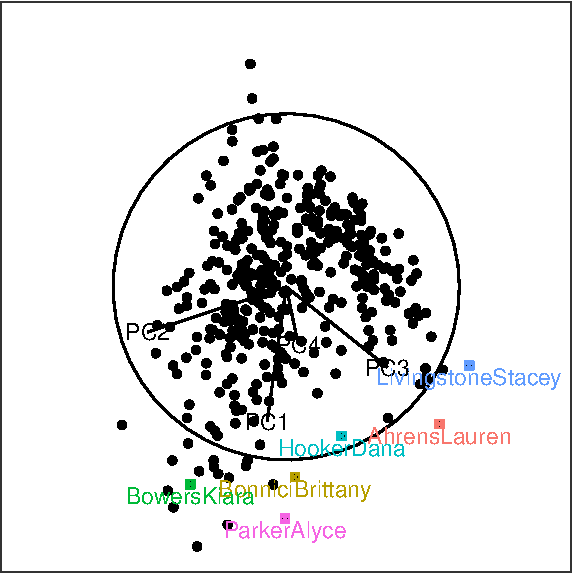
\includegraphics[width=0.6\linewidth,height=\textheight,keepaspectratio]{4-pca_files/figure-pdf/fig-aflw-pcaplots-pdf-1.pdf}

}

\caption{\label{fig-aflw-pcaplots-pdf}Frame 18 re-plotted so that
players can be identified. Here some players are labelled, but ideally
this plot is interactive and any player can be identified.
\faIcon{play-circle}}

\end{figure}%

For any particular frame, like 18 re-plotted in
Figure~\ref{fig-aflw-pcaplots-pdf}, we can investigate further. Here
there is a branching pattern, where the branch points in the direction
of PC 1. Mouse-over the players at the tip of this branch and we find
players like Alyce Parker, Brittany Bonnici, Dana Hooker, Kiara Bowers.
If you look up the bios of these players you'll find they all have
generally good player descriptions like ``elite disposals'', ``powerful
left foot'', ``hard-running midfielder'', ``best and fairest''.

In the direction of PC 2, you'll find players like Lauren Ahrens, Stacey
Livingstone who are star defenders. Players in this end of PC 2, have
high scores on \texttt{intercepts} and \texttt{rebounds\_in50}.

Another interesting frame for inspecting PC 2 is 59. PC 2 at one end has
players with high goal scoring skills, and the other good defending
skills. So mousing over the other end of PC 2 finds players like Gemma
Houghton and Katie Brennan who are known for their goal scoring. The
branch pattern is an interesting one, because it tells us there is some
combination of skills that are lacking among all players, primarily this
appears to be there some distinction between defenders skills and
general playing skills. It's not as simple as this because the branching
is only visible when PC 1 and PC 2 are examined with PC 3.

PCA is useful for getting a sense of the variation in a high-dimensional
data set. Interpreting the principal components is often useful, but it
can be discombobulating. For the \texttt{aflw} data it would be good to
think about it as a guide to the main directions of variation and to
follow with a more direct engineering of variables into interesting
player characteristics. For example, calculate offensive skill as an
equal combination of goals, accuracy, shots, behinds. A set of new
variables specifically computed to measure particular skills would make
explaining an analysis easier.

\insightbox{The tour verifies that PCA on the `aflw` data is complicated and doesn't capture all of the variation. However, it does provide useful insights. It detected outstanding players, and indicated the different skills sets of top goal scorers and top defensive players.}

\section{Examining the PCA model in the data
space}\label{examining-the-pca-model-in-the-data-space}

\index{model-in-the-data-space}

When you choose a smaller number of PCs \((k)\) than the number of
original variables, this is essentially producing a model for the data.
The model is the lower dimensional \(k\)-D space. It is analogous to a
linear regression model, except that the residuals from the model are
\((p-k)\)-D.

It is common to show the model, that is the data projected into the
\(k\)-D model space. When \(k=2\) this is called a ``biplot''. For the
\texttt{plane} and \texttt{plane\_noise} data the biplots are shown in
Figure~\ref{fig-plane-biplot}. This is useful for checking which
variables contribute most to the new principal component variables, and
also to check for any problems that might have affected the fit, such as
outliers, clusters or non-linearity. Interestingly, biplots are
typically only made in 2D, even if the data should be summarised by more
than two PCs. Occasionally you will see the biplot made for PC \(j\) vs
PC \(k\) also. With the \texttt{pca\_tour()} function in the
\texttt{tourr} package you can view a \(k\)-D biplot. This will display
the \(k\) PCs with the axes displaying the original variables, and thus
show their contribution to the PCs.

\begin{figure}

\centering{

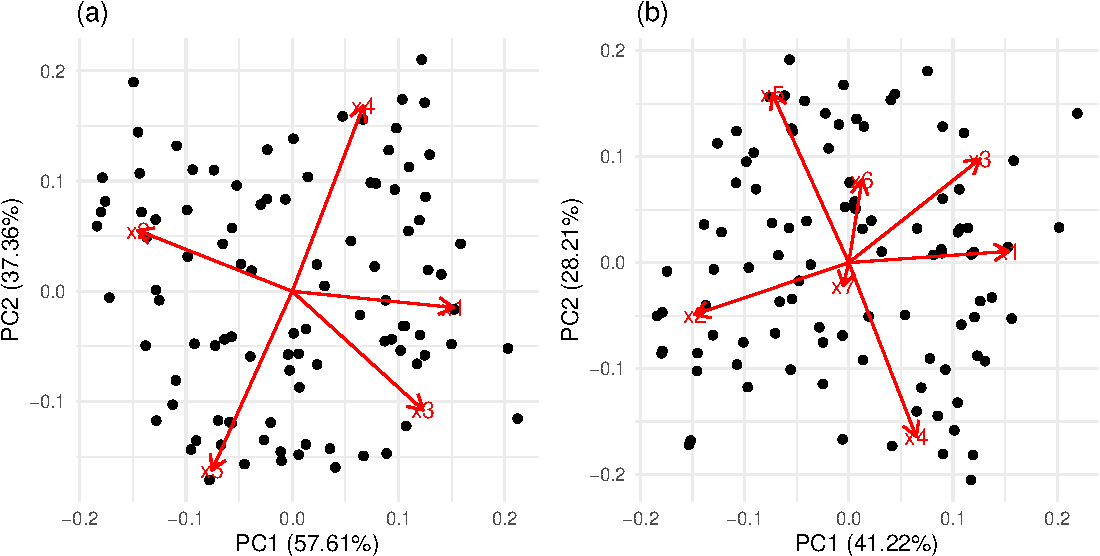
\includegraphics[width=1\linewidth,height=\textheight,keepaspectratio]{4-pca_files/figure-pdf/fig-plane-biplot-1.pdf}

}

\caption{\label{fig-plane-biplot}Biplots of the plane (a) and plane +
noise (b) data. All five variables contribute strongly to the two
principal components in (a): PC1 is primarily \texttt{x1}, \texttt{x2}
and \texttt{x3} and PC2 is primarily \texttt{x4} and \texttt{x5}. In (b)
the same four variables contribute in almost the same way, with
variables \texttt{x6} and \texttt{x7} contributing very little. The data
was constructed this way, that these two dimensions were purely noise.}

\end{figure}%

It can be useful to examine this model using the tour. The model is
simply a plane in high dimensions. This would be considered to be the
model in the data space. The reason to do this is to check how well the
model fits the data. The plane corresponding to the model should be
oriented along the main direction of the points, and the spread of
points around the plane should be small. We should also be able to see
if there has been any strong non-linear relationship missed by the
model, or outliers and clusters.

The function \texttt{pca\_model()} from the \texttt{mulgar} package can
be used to represent the model as a \(k\)-D wire-frame plane.
Figure~\ref{fig-plane-box-model-pdf} shows the models for the
\texttt{plane} and \texttt{box} data, 2D and 3D respectively.

\infobox{We look at the model in the data space to check how well the model fits the data. If it fits well, the points will cluster tightly around the model representation, with little spread in other directions.}

\begin{figure}

\begin{minipage}{0.50\linewidth}

\centering{

\pandocbounded{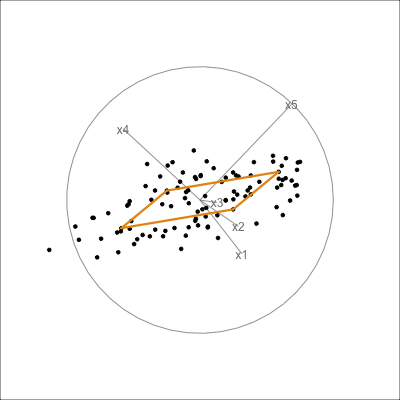
\includegraphics[keepaspectratio]{images/plane_model_55.png}}

}

\subcaption{\label{fig-plane-model}Model for the 2D in 5D data.}

\end{minipage}%
%
\begin{minipage}{0.50\linewidth}

\centering{

\pandocbounded{\includegraphics[keepaspectratio]{images/box_model_13.png}}

}

\subcaption{\label{fig-box-model}Model for the 3D in 5D data.}

\end{minipage}%

\caption{\label{fig-plane-box-model-pdf}PCA model overlaid on the data
for the 2D in 5D, and 3D in 5D simulated data. \faIcon{play-circle}}

\end{figure}%

\subsection{Example: pisa}\label{example-pisa-1}

\index{data!pisa}

The model for the \texttt{pisa} data is a 1D vector, shown in
Figure~\ref{fig-pisa-model-pdf}. In this example there is a good
agreement between the model and the data.

\begin{figure}

\centering{

\includegraphics[width=3.125in,height=\textheight,keepaspectratio]{images/pisa_model_17.png}

}

\caption{\label{fig-pisa-model-pdf}PCA model of the \texttt{pisa} data.
The 1D model captures the primary variation in the data and there is a
small amount of spread in all directions away from the model.
\faIcon{play-circle}}

\end{figure}%

\insightbox{The `pisa` data fits fairly closely to the 1D PCA model. The variance of points away from the model is symmetric and relatively small. These suggest the 1D model is a reasonably summary of the test scores.}

\subsection{Example: aflw}\label{example-aflw-1}

\index{data!aflw}

It is less useful to examine the PCA model for the \texttt{aflw} data,
because the main patterns that were of interest were the exceptional
players. However, we will do it anyway! Figure~\ref{fig-aflw-model-pdf}
shows the 4D PCA model overlain on the data. Even though the
distribution of points is not as symmetric and balanced as the other
examples, we can see that the cube structure mirrors the variation. We
can see that the relationships between variables are not strictly
linear, because the spread extends unevenly away from the box.

\begin{figure}

\centering{

\includegraphics[width=3.125in,height=\textheight,keepaspectratio]{images/aflw_model_70.png}

}

\caption{\label{fig-aflw-model-pdf}PCA model of the \texttt{aflw} data.
The linear model is not ideal for this data, which has other patterns
like outliers, and some branching. However, the model roughly captures
the linear associations, and leaves unexplained variation in different
directions. \faIcon{play-circle}}

\end{figure}%

\insightbox{From the tour we see that the 4D model leaves substantial variation unexplained. It is also not symmetric, and there is some larger variation away from the model in some combinations of variables than others.}

\section{When relationships are not
linear}\label{when-relationships-are-not-linear}

\subsection{Example: outliers}\label{example-outliers}

\index{outliers}

Figure~\ref{fig-plane-n-o-scree} shows the scree plot for the planar
data with noise and outliers. It is very similar to the scree plot on
the data without the outliers (Figure~\ref{fig-plane-noise-scree}).
However, what we see from Figure~\ref{fig-p-o-pca-pdf} is that PCA loses
the outliers. The animation in (a) shows the full data, and the outliers
marked by colour and labels 1, 2, are clearly unusual in some
projections. When we examine the tour of the first four PCs (as
suggested by the scree plot) the outliers are not unusual. They are
almost contained in the point cloud. The reason is clear when all the
PCs are plotted, and the outliers can be seen to be clearly detected
only in PC5, PC6 and PC7.

\begin{Shaded}
\begin{Highlighting}[]
\NormalTok{plane\_n\_o\_pca }\OtherTok{\textless{}{-}} \FunctionTok{prcomp}\NormalTok{(plane\_noise\_outliers)}
\FunctionTok{ggscree}\NormalTok{(plane\_n\_o\_pca, }\AttributeTok{q =} \DecValTok{7}\NormalTok{) }\SpecialCharTok{+} \FunctionTok{theme\_minimal}\NormalTok{()}
\end{Highlighting}
\end{Shaded}

\begin{figure}[H]

\centering{

\includegraphics[width=0.8\linewidth,height=\textheight,keepaspectratio]{4-pca_files/figure-pdf/fig-plane-n-o-scree-1.pdf}

}

\caption{\label{fig-plane-n-o-scree}Scree plot of the planar data with
noise and an outlier. It is almost the same as the data without the
outliers.}

\end{figure}%

\begin{figure}

\begin{minipage}{0.50\linewidth}

\centering{

\includegraphics[width=2.1875in,height=\textheight,keepaspectratio]{images/plane_n_o_clr_181.png}

}

\subcaption{\label{fig-plane-n-o-clr}Outliers clearly visible}

\end{minipage}%
%
\begin{minipage}{0.50\linewidth}

\centering{

\includegraphics[width=2.1875in,height=\textheight,keepaspectratio]{images/plane_n_o_pca_181.png}

}

\subcaption{\label{fig-plane-n-o-pca}Outliers not clearly visible in
PC1-4}

\end{minipage}%

\caption{\label{fig-p-o-pca-pdf}Examining the handling of outliers in
the PCA of the planar data with noise variables and two outliers. PCA
has lost these two extreme values. \faIcon{play-circle}}

\end{figure}%

\begin{figure}

\centering{

\includegraphics[width=0.8\linewidth,height=\textheight,keepaspectratio]{4-pca_files/figure-pdf/fig-plane-o-n-pairs-1.pdf}

}

\caption{\label{fig-plane-o-n-pairs}From the scatterplot matrix we can
see that the outliers are present in PC5, PC6 and PC7. That means by
reducing the dimensionality to the first four PCs the model has missed
some important characteristics in the data.}

\end{figure}%

\subsection{Example: Non-linear
associations}\label{example-non-linear-associations}

\index{nonlinearity}

Figure~\ref{fig-plane-nonlin-pdf} shows the tour of the full 5D data
containing non-linear relationships in comparison with a tour of the
first three PCs, as recommended by the scree plot
(Figure~\ref{fig-plane-nonlin-scree}). The PCs capture some clear and
very clean non-linear relationship, but it looks like it has missed some
of the complexities of the relationships. The scatterplot matrix of all
5 PCs (Figure~\ref{fig-plane-nonlin-pairs}) shows that PC4 and PC5
contain interesting features: more non-linearity, and curiously an
outlier.

\begin{figure}

\centering{

\includegraphics[width=0.8\linewidth,height=\textheight,keepaspectratio]{4-pca_files/figure-pdf/fig-plane-nonlin-scree-1.pdf}

}

\caption{\label{fig-plane-nonlin-scree}Scree plot of the non-linear data
suggests three PCs.}

\end{figure}%

\begin{figure}

\begin{minipage}{0.50\linewidth}

\centering{

\includegraphics[width=2.1875in,height=\textheight,keepaspectratio]{images/plane_nonlin.png}

}

\subcaption{\label{fig-nonlinear2}All five variables}

\end{minipage}%
%
\begin{minipage}{0.50\linewidth}

\centering{

\includegraphics[width=2.1875in,height=\textheight,keepaspectratio]{images/plane_nonlin_pca_129.png}

}

\subcaption{\label{fig-plane-nonlin-pca}First three PCs}

\end{minipage}%

\caption{\label{fig-plane-nonlin-pdf}Comparison of the full data and
first three principal components. Non-linear relationships between
several variables can be seen in a tour on all five variables. The first
three principal components reveal a strong non-linear relationship. Some
of the non-linearity is clearly visible in the reduced dimension space,
but the full data has more complexities. \faIcon{play-circle}}

\end{figure}%

\begin{figure}

\centering{

\includegraphics[width=0.8\linewidth,height=\textheight,keepaspectratio]{4-pca_files/figure-pdf/fig-plane-nonlin-pairs-1.pdf}

}

\caption{\label{fig-plane-nonlin-pairs}From the scatterplot matrix we
can see that the there is a non-linear relationship visible in PC1 and
PC2, with perhaps a small contribution from PC3. However, we can see
that when the data is reduced to three PCs, it misses catching all on
the non-linear relationships and also interestingly it seems that there
is an unusual observation also.}

\end{figure}%

\infobox{One of the dangers of PCA is that interesting and curious details of the data can captured by the lowest PCs, that are usually discarded. The tour, and examining the smaller PCs, can help to discover them.}

\section*{Exercises}\label{exercises-3}
\addcontentsline{toc}{section}{Exercises}

\markright{Exercises}

\begin{enumerate}
\def\labelenumi{\arabic{enumi}.}
\tightlist
\item
  Make a scatterplot matrix of the first four PCs of the \texttt{aflw}
  data. Is the branch pattern visible in any pair?
\item
  Construct five new variables to measure these skills offense, defense,
  playing time, ball movement, errors. Using the tour, examine the
  relationship between these variables. Map out how a few players could
  be characterised based on these directions of skills.
\item
  Symmetrise any \texttt{aflw} variables that have skewed distributions
  using a log or square root transformation. Then re-do the PCA. What do
  we learn that is different about associations between the skill
  variables?
\item
  Examine the \texttt{bushfires} data using a grand tour on the numeric
  variables, ignoring the \texttt{cause} (class) variable. Note any
  issues such as outliers, or skewness that might affect PCA. How many
  principal components would be recommended by the scree plot? Examine
  this PCA model with the data, and explain how well it does or doesn't
  fit.
\item
  Use the \texttt{pca\_tour} to examine the first five PCs of the
  \texttt{bushfires} data. How do all of the variables contribute to
  this reduced space?
\item
  Reduce the dimension of the \texttt{sketches} data to 12 PCs. How much
  variation does this explain? Is there any obvious clustering in this
  lower dimensional space?
\item
  Copulas are commonly used to define the covariance relationship
  between pairs of variables, for fixed marginal distributions. There
  are several R packages that enable simulating multivariate data using
  copula methods.
\end{enumerate}

\begin{enumerate}
\def\labelenumi{\alph{enumi}.}
\tightlist
\item
  Use the \texttt{covsim} package to simulate data. The following code
  will generate 5D data with normal marginal distributions.
\end{enumerate}

\begin{Shaded}
\begin{Highlighting}[]
\FunctionTok{library}\NormalTok{(covsim)}
\FunctionTok{library}\NormalTok{(tidyverse)}
\FunctionTok{library}\NormalTok{(tourr)}
\FunctionTok{set.seed}\NormalTok{(}\DecValTok{308}\NormalTok{) }\CommentTok{\# define a target covariance}
\NormalTok{p }\OtherTok{\textless{}{-}} \DecValTok{5}
\CommentTok{\# Basically randomise the target covariance bc small sample}
\NormalTok{sigma.target }\OtherTok{\textless{}{-}} \FunctionTok{cov}\NormalTok{(MASS}\SpecialCharTok{::}\FunctionTok{mvrnorm}\NormalTok{(}\DecValTok{10}\NormalTok{, }\AttributeTok{mu=}\FunctionTok{rep}\NormalTok{(}\DecValTok{0}\NormalTok{, p), }\AttributeTok{Sigma=}\FunctionTok{diag}\NormalTok{(}\DecValTok{1}\NormalTok{, p)))}
\CommentTok{\# normal margins that match the covariances:}
\NormalTok{marginsnorm }\OtherTok{\textless{}{-}} \FunctionTok{lapply}\NormalTok{(}\AttributeTok{X=}\FunctionTok{sqrt}\NormalTok{(}\FunctionTok{diag}\NormalTok{(sigma.target)),}\ControlFlowTok{function}\NormalTok{(X) }\FunctionTok{list}\NormalTok{(}\AttributeTok{distr=}\StringTok{"norm"}\NormalTok{, }\AttributeTok{sd=}\NormalTok{X) )}
\NormalTok{calibrated.vine }\OtherTok{\textless{}{-}} \FunctionTok{vita}\NormalTok{(marginsnorm, }\AttributeTok{sigma.target =}\NormalTok{sigma.target, }\AttributeTok{Nmax=}\DecValTok{10}\SpecialCharTok{\^{}}\DecValTok{5}\NormalTok{, }\AttributeTok{cores=}\DecValTok{1}\NormalTok{)}
\NormalTok{copdata }\OtherTok{\textless{}{-}}\NormalTok{ rvinecopulib}\SpecialCharTok{::}\FunctionTok{rvine}\NormalTok{(}\DecValTok{467}\NormalTok{, calibrated.vine)}
\NormalTok{copdata }\OtherTok{\textless{}{-}} \FunctionTok{as.data.frame}\NormalTok{(copdata)}
\NormalTok{GGally}\SpecialCharTok{::}\FunctionTok{ggscatmat}\NormalTok{(copdata)}
\FunctionTok{cov}\NormalTok{(copdata)}
\NormalTok{sigma.target}
\FunctionTok{animate\_xy}\NormalTok{(copdata)}
\end{Highlighting}
\end{Shaded}

\begin{enumerate}
\def\labelenumi{\alph{enumi}.}
\setcounter{enumi}{1}
\tightlist
\item
  The \texttt{ecoCopula} package has a function \texttt{simulate} that
  can generate data similar to ecological abundance data using
  discretized copulas.
\end{enumerate}

\begin{Shaded}
\begin{Highlighting}[]
\FunctionTok{library}\NormalTok{(ecoCopula)}
\FunctionTok{data}\NormalTok{(spider)}
\NormalTok{abund }\OtherTok{\textless{}{-}}\NormalTok{ spider}\SpecialCharTok{$}\NormalTok{abund}
\NormalTok{spider\_mod\_ssdm }\OtherTok{=} \FunctionTok{stackedsdm}\NormalTok{(abund,}\SpecialCharTok{\textasciitilde{}}\DecValTok{1}\NormalTok{, }\AttributeTok{data =}\NormalTok{ spider}\SpecialCharTok{$}\NormalTok{x, }\AttributeTok{ncores=}\DecValTok{2}\NormalTok{)}
\NormalTok{spid\_lv\_ssdm }\OtherTok{=} \FunctionTok{cord}\NormalTok{(spider\_mod\_ssdm)}
\NormalTok{spider\_sim }\OtherTok{\textless{}{-}} \FunctionTok{simulate}\NormalTok{(spid\_lv\_ssdm, }\AttributeTok{nsim=}\DecValTok{1}\NormalTok{, }\AttributeTok{seed=}\DecValTok{1001}\NormalTok{)}
\end{Highlighting}
\end{Shaded}

\section*{Project}\label{project-1}
\addcontentsline{toc}{section}{Project}

\markright{Project}

Linear dimension reduction can optimise for other criteria, and here we
will explore one example: the algorithm (Kandanaarachchi \& Hyndman,
2021) implemented in the \texttt{dobin} package (Kandanaarachchi, 2022)
finds a basis in which the first few directions are optimized for the
detection of outliers in the data. We will examine how it performs for
the \texttt{plane\_noise\_outliers} data (the example where outliers
were hidden in the first four principal components.)

\begin{enumerate}
\def\labelenumi{\arabic{enumi}.}
\tightlist
\item
  Start by looking up the documentation of \texttt{dobin::dobin}. How
  many parameters does the method depend on?
\item
  We first apply the function to the \texttt{plane\_noise\_outliers}
  data using default values for all parameters.
\item
  Recall that the outliers were added in rows 101 and 102 of the data.
  Make a scatter plots showing the projection onto the first, second and
  third component found by \texttt{dobin}, using color to highlight the
  outliers. Are they visible as outliers with three components?
\item
  Adjust the \texttt{frac} parameter of the \texttt{dobin} function to
  \texttt{frac\ =\ 0.99} and repeat the graphical evaluation from point
  3. How does it compare to the previous solution?
\end{enumerate}

\chapter{Non-linear dimension
reduction}\label{non-linear-dimension-reduction}

Non-linear dimension reduction (NLDR) aims to find a single
low-dimensional representation of the high-dimensional data that shows
the main features of the data. If there are separated clusters present
then it might be a layout where the clusters are all distinct, in a way
that a single linear projection could not reveal. For observations
falling on a low-dimensional non-linear manifold in high dimensions the
NLDR might unfold or unroll it so that they are represented in a plane
where the distances are similar to their distance along the manifold.

\index{manifold} \index{interpoint distance}

Most techniques only require an interpoint similarity or distance matrix
as the main ingredient, rather than the full \(p\)-dimensional data. A
classic example where only this information is the morse code data
reported by Rothkopf (1957a), and available in the \texttt{xgobi}
software (Swayne et al., 1998). The data contains the counts of the
number of times that a letter is mistaken for another letter collected
in an experimental study. However, here we focus on problems where the
full \(p\)-dimensional data is available, so we can also compare
structure perceived using the tour on the high-dimensional space,
relative to structure revealed in the low-dimensional embedding.

\infobox{A common myth is that non-linear dimension reduction captures non-linear patterns in the high-dimensional data. It may or may not do this. The term means that the methods transform the data non-linearly into a useful (or not) visual representation.}

\section{Classical methods}\label{classical-methods}

In statistics, methods for non-linear dimension reduction arise with
multidimensional scaling (MDS) (Kruskal, 1964a). Classically, MDS
minimises some function of the difference between two interpoint
distance matrices, the distance between points in the high-dimensions,
and in the low-dimensional representations using a stress function
(\(C_{L2}\)):

\[
C_{L2} = \left(\sum_{i, j=1; i\neq j}^n (d_p(i,j) - d_k(i,j))^2\right)^{1/2}
\] where \((d_p(i,j))\) are the distances between all pairs of points in
\(p\)-dimensions, and \(d_k(i,j)\) is the distance between the points in
the low-dimensional (\(k\)) space. PCA is a special case of MDS, in
that, the first two PCs provide the solution to the above equation if
distance is Euclidean. Each PC is a linear projection, but generally MDS
can provide non-linear transformations to represent unusual
high-dimensional patterns.

The choices for defining \(d_p\) are many, including ones that are
locally, using say \(k\) nearest neighbours, or globally computed.
Distances can also be transformed using some function, including ranks
instead of actual distance. Another approach modifies the stress
function the \(L_2\)-norm, by replacing the 2 with an arbitrary power.
Others yet use transformations of the distances. A good resource for
learning about MDS and the many choices is Borg \& Groenen (2005).

\index{data!swiss roll}

The methods \emph{isomap} (Tenenbaum et al., 2000) and \emph{local
linear embedding} (LLE) are two methods where local distance is used,
and they were designed to unwrap data from a manifold.
Figure~\ref{fig-swiss-pdf} illustrates how the results on the classic
swiss roll data can differ according to method, in useful ways. The
observations lie on a 2D non-linear manifold in 3D. The data is a
manufactured example introduced to illustrate the ability of isomap and
LLE to unwrap the swiss roll and lay out the points in a rectangle as
though one was travelling along the surface.

\index{software!Rdimtools} \index{software!cardinalR}
\index{dimension reduction!isomap}
\index{dimension reduction!local linear embedding (LLE)}

\begin{figure}

\begin{minipage}{0.33\linewidth}

\includegraphics[width=1.48958in,height=\textheight,keepaspectratio]{images/swiss.png}

\subcaption{\label{}tour}
\end{minipage}%
%
\begin{minipage}{0.33\linewidth}

\includegraphics[width=1\linewidth,height=\textheight,keepaspectratio]{5-nldr_files/figure-pdf/unnamed-chunk-4-1.pdf}

\subcaption{\label{}PCA}
\end{minipage}%
%
\begin{minipage}{0.33\linewidth}

\includegraphics[width=1\linewidth,height=\textheight,keepaspectratio]{5-nldr_files/figure-pdf/unnamed-chunk-5-1.pdf}

\subcaption{\label{}isomap}
\end{minipage}%

\caption{\label{fig-swiss-pdf}The classic swiss roll data constructed to
illustrate isomap, as shown in (a) a random tour projection, (b) lowest
two principal components, (c) NLDR provided by isomap. The spiral can be
discovered by many methods, including different principal compoents
depending on the scaling of the data, or using projection pursuit, or
nonlinear MDS. Being able to unwrap the spiral and lay out the points
along a plane is achieved by isomap and LLE with careful choice of
parameters. Colour indicates distance along this spiral.
\faIcon{play-circle}}

\end{figure}%

\index{dimension reduction!MDS} \index{dimension reduction!t-SNE}
\index{dimension reduction!UMAP}

The swiss roll data is interesting in the sense that from a visual
perspective it is interesting to be able to \emph{discover} the spiral
structure. Particularly this would be a more challenging if the 2D
spiral was in data with more than three variables, and all the
additional ones were noise (like \texttt{z} in this example). Methods
like projection pursuit, PCA or MDS can discover the spiral if all
variables are measured on the same scale (say -1, 1) but not
standardised because the variance of the spiral shape is different from
that of noise. Being able to discover the manifold (here, a 2D surface
matching a swiss roll) can be useful for conducting further analysis.
The points are now organised according to distance relative to the
manifold on which they live. This layout is like taming a lion, it feels
like an achievement, but realistically it is very difficult to achieve
from these methods: data scale choice or a different number of \(k\)
nearest neighbours, changes the layout dramatically. Organising the
points into distance along the spiral could have equally been achieved
by discovering the spiral, and computing radial distance, as done to
produce the colouring of points in Figure~\ref{fig-swiss-pdf}. This
approach would also extend beyond 3D, to any additional number of noise
dimensions.

\section{Contemporary approaches}\label{contemporary-approaches}

\index{software!uwot} \index{software!Rtsne}

\begin{figure}

\centering{

\includegraphics[width=1\linewidth,height=\textheight,keepaspectratio]{5-nldr_files/figure-pdf/fig-nldr-clusters-1.pdf}

}

\caption{\label{fig-nldr-clusters}Two non-linear embeddings of the
non-linear clusters data: (a) t-SNE, (b) UMAP. One suggests five
clusters and the other four, and also disagree on the cluster shapes.}

\end{figure}%

Popular methods in current use for NLDR include t-SNE (Maaten \& Hinton,
2008) and UMAP (McInnes et al., 2018). These approaches use a different
approach for comparing the high-dimensional and low-dimensional
distances, based on Kullback-Leibler divergence:

\[
C_{KL} = \sum_{i,j} p_{ij}\log\left(\frac{p_{ij}}{q_{ij}}\right)
\] where \(i,j\) indicate two observations in the data, and
\(p_{ij}, q_{ij}\) are the probability distributions of the distances in
\(p\) and \(k\) dimensions, respectively. To obtain \(p_{ij}\) the
interpoint distances are computed, and normalised by dividing by
\(\sum_{i,j} p_{ij}\), as is done similarly to obtain \(q_{ij}\). A
further step in t-SNE is transforming the distances through the CDF of a
specified distribution (Gaussian in \(p\)-D and \(t\)-distribution in
\(k\)-D) to reflect differences is volume between the high and low
dimensional spaces, akin to the transformation used in the sage tour
(Laa et al. (2022)). (See Figure~\ref{fig-density} illustrating the
crowding effect.) The normalisation effectively means small distances,
like distances between points that are in a cluster, even if clusters
are bigger or smaller, become relatively closer in comparison with all
the large distances.

In practice, the optimisation is conducted with a likelihood function:

\[
C_{LV} = \sum_{i \neq j} p_{ij} \log\left(w_{ij}\right) + \gamma \sum_{i \neq j} \log\left(w_{ij}\right)
\] where \(w_{ij}\) are the unnormalised similarities in the
\(k\)-dimensional representation, and the second component weighted by
\(\gamma\) adds a repulsive force to push points apart. UMAP optimises a
variation of \(C_{LV}\). Both t-SNE and UMAP are designed with cluster
structure in mind, and may provide useful low-dimensional
representations of clustering in high-dimensions.

Figure~\ref{fig-nldr-clusters} shows two NLDR views of the
\texttt{clusters\_nonlin} data set from the \texttt{mulgar} package.
Both suggest that there are four clusters, and that some clusters are
non-linearly shaped. They disagree on the type of non-linear pattern,
where t-SNE represents one cluster as a wavy-shape and UMAP both have a
simple parabolic shape.

\begin{figure}

\begin{minipage}{0.50\linewidth}
\includegraphics[width=2.29167in,height=\textheight,keepaspectratio]{images/clusters_nonlin_60.png}\end{minipage}%
%
\begin{minipage}{0.50\linewidth}
\includegraphics[width=2.29167in,height=\textheight,keepaspectratio]{images/clusters_nonlin_272.png}\end{minipage}%

\caption{\label{fig-clusters-nonlin-pdf}Two frames from a grand tour of
the nonlinear clusters data set, shows four clusters. Two are very small
and spherical in shape. One is large, and has a sine wave shape, and the
other is fairly small with a bent rod shape. \faIcon{play-circle}}

\end{figure}%

The full 4D data is shown with a grand tour in
Figure~\ref{fig-clusters-nonlin-pdf}. The four clusters suggested by the
NLDR methods can be seen. We also get a better sense of the relative
size and proximity of the clusters. There are two small spherical
clusters, one quite close to the end of the large sine wave cluster. The
fourth cluster is relatively small, and has a slight curve, like a bent
rod. The t-SNE representation is slightly more accurate than the UMAP
representation. We would expect that the wavy cluster is the sine wave
seen in the tour.

\infobox{NLDR can provide useful low-dimensional summaries of high-dimensional structure but you need to check whether it is a sensible and accurate representation by comparing with what is perceived from a tour.}

\section{Assessing an NLDR layout}\label{assessing-an-nldr-layout}

Figure~\ref{fig-nldr-clusters} shows that NLDR can produce useful
low-dimensional summaries of structure in high-dimensional data.
However, it can be a frustrating exercise because \textbf{very
different} representations can result depending on the parameter
choices, and even the random number seeding the fit. (You can check this
by changing the \texttt{set.seed} in the code above, and by changing
from the default parameters.) Also, it may not be possible to represent
the high-dimensional structures faithfully in low dimensions.

Diagnosing a layout is an important first step to determine if it can be
appropriately used in further analysis. The approach for doing this date
back to the methods discussed in Buja et al. (2008). The NLDR view needs
to be interactively linked to other plots of the data, and especially to
a tour with the specific purpose to determine the faithfulness to the
structure present in high dimensions. For example, with the data in
Figure~\ref{fig-nldr-clusters}, we would want to know which of the two
curved clusters in the UMAP representation correspond to the sine wave
cluster.

\subsection{\texorpdfstring{Using
\texttt{liminal}}{Using liminal}}\label{using-liminal}

\index{software!liminal}

Figure~\ref{fig-liminal-clusters-nonlin} shows how the NLDR plot can be
linked to a tour view, using the \texttt{liminal} package, to better
understand how well the structure of the data is represented. Here we
learn that the smile in the UMAP embedding is the small bent rod
cluster, and that the unibrow is the sine wave.

\begin{Shaded}
\begin{Highlighting}[]
\FunctionTok{library}\NormalTok{(liminal)}
\NormalTok{umap\_df }\OtherTok{\textless{}{-}} \FunctionTok{data.frame}\NormalTok{(}\AttributeTok{umapX =}\NormalTok{ cnl\_umap[, }\DecValTok{1}\NormalTok{],}
                      \AttributeTok{umapY =}\NormalTok{ cnl\_umap[, }\DecValTok{2}\NormalTok{])}
\FunctionTok{limn\_tour\_link}\NormalTok{(}
\NormalTok{  umap\_df,}
\NormalTok{  clusters\_nonlin,}
  \AttributeTok{cols =}\NormalTok{ x1}\SpecialCharTok{:}\NormalTok{x4}
\NormalTok{)}
\end{Highlighting}
\end{Shaded}

\begin{figure}

\begin{minipage}{\linewidth}

\centering{

\pandocbounded{\includegraphics[keepaspectratio]{images/liminal-clusters-nonlin1.png}}

}

\subcaption{\label{fig-smile}Smile matches bent rod.}

\end{minipage}%
\newline
\begin{minipage}{\linewidth}

\centering{

\pandocbounded{\includegraphics[keepaspectratio]{images/liminal-clusters-nonlin2.png}}

}

\subcaption{\label{fig-unibrow}Unibrow matches sine wave.}

\end{minipage}%

\caption{\label{fig-liminal-clusters-nonlin}Two screenshots from liminal
showing which clusters match between the UMAP representation and the
tour animation. The smile corresponds to the small bent rod cluster. The
unibrow matches to the sine wave cluster.}

\end{figure}%

\subsection{\texorpdfstring{Using
\texttt{detourr}}{Using detourr}}\label{using-detourr}

\index{software!detourr} \index{software!crosstalk}
\index{software!plotly}

Figure~\ref{fig-detourr-clusters-nonlin} shows how the linking is
achieved using \texttt{detourr}. It uses a shared data object, as made
possible by the \texttt{crosstalk} package, and the UMAP view is made
interactive using \texttt{plotly}.

\begin{Shaded}
\begin{Highlighting}[]
\FunctionTok{library}\NormalTok{(detourr)}
\FunctionTok{library}\NormalTok{(dplyr)}
\FunctionTok{library}\NormalTok{(crosstalk)}
\FunctionTok{library}\NormalTok{(plotly)}
\NormalTok{umap\_df }\OtherTok{\textless{}{-}} \FunctionTok{data.frame}\NormalTok{(}\AttributeTok{umapX =}\NormalTok{ cnl\_umap[, }\DecValTok{1}\NormalTok{],}
                      \AttributeTok{umapY =}\NormalTok{ cnl\_umap[, }\DecValTok{2}\NormalTok{])}
\NormalTok{cnl\_df }\OtherTok{\textless{}{-}} \FunctionTok{bind\_cols}\NormalTok{(clusters\_nonlin, umap\_df)}
\NormalTok{shared\_cnl }\OtherTok{\textless{}{-}}\NormalTok{ SharedData}\SpecialCharTok{$}\FunctionTok{new}\NormalTok{(cnl\_df)}

\NormalTok{detour\_plot }\OtherTok{\textless{}{-}} \FunctionTok{detour}\NormalTok{(shared\_cnl, }\FunctionTok{tour\_aes}\NormalTok{(}
  \AttributeTok{projection =} \FunctionTok{starts\_with}\NormalTok{(}\StringTok{"x"}\NormalTok{))) }\SpecialCharTok{|\textgreater{}}
    \FunctionTok{tour\_path}\NormalTok{(}\FunctionTok{grand\_tour}\NormalTok{(}\DecValTok{2}\NormalTok{), }
                    \AttributeTok{max\_bases=}\DecValTok{50}\NormalTok{, }\AttributeTok{fps =} \DecValTok{60}\NormalTok{) }\SpecialCharTok{|\textgreater{}}
       \FunctionTok{show\_scatter}\NormalTok{(}\AttributeTok{alpha =} \FloatTok{0.7}\NormalTok{, }\AttributeTok{axes =} \ConstantTok{FALSE}\NormalTok{,}
                    \AttributeTok{width =} \StringTok{"100\%"}\NormalTok{, }\AttributeTok{height =} \StringTok{"450px"}\NormalTok{)}

\NormalTok{umap\_plot }\OtherTok{\textless{}{-}} \FunctionTok{plot\_ly}\NormalTok{(shared\_cnl,}
                    \AttributeTok{x =} \SpecialCharTok{\textasciitilde{}}\NormalTok{umapX, }
                    \AttributeTok{y =} \SpecialCharTok{\textasciitilde{}}\NormalTok{umapY,}
                    \AttributeTok{color =} \FunctionTok{I}\NormalTok{(}\StringTok{"black"}\NormalTok{),}
                    \AttributeTok{height =} \DecValTok{450}\NormalTok{) }\SpecialCharTok{\%\textgreater{}\%}
    \FunctionTok{highlight}\NormalTok{(}\AttributeTok{on =} \StringTok{"plotly\_selected"}\NormalTok{, }
              \AttributeTok{off =} \StringTok{"plotly\_doubleclick"}\NormalTok{) }\SpecialCharTok{\%\textgreater{}\%}
    \FunctionTok{add\_trace}\NormalTok{(}\AttributeTok{type =} \StringTok{"scatter"}\NormalTok{, }
              \AttributeTok{mode =} \StringTok{"markers"}\NormalTok{)}

\FunctionTok{bscols}\NormalTok{(}
\NormalTok{     detour\_plot, umap\_plot,}
     \AttributeTok{widths =} \FunctionTok{c}\NormalTok{(}\DecValTok{5}\NormalTok{, }\DecValTok{6}\NormalTok{)}
\NormalTok{ )}
\end{Highlighting}
\end{Shaded}

\begin{figure}

\centering{

\pandocbounded{\includegraphics[keepaspectratio]{images/detourr-clusters-nonlin.png}}

}

\caption{\label{fig-detourr-clusters-nonlin}Screenshot from detourr
showing which clusters match between the UMAP representation and the
tour animation. The smile corresponds to the small bent rod cluster.}

\end{figure}%

\section{\texorpdfstring{Example:
\texttt{fake\_trees}}{Example: fake\_trees}}\label{example-fake_trees}

\index{data!fake trees}

Figure~\ref{fig-liminal-trees} shows a more complex example, using the
\texttt{fake\_trees} data. We know that the 10D data has a main branch,
and 9 branches (clusters) attached to it, based on our explorations in
the earlier chapters. The t-SNE view, where points are coloured by the
known branch ids, is very helpful for seeing the linear branch
structure.

What we can't tell is that there is a main branch from which all of the
others extend. We also can't tell which of the clusters corresponds to
this branch. Linking the plot with a tour helps with this. Although, not
shown in the sequence of snapshots in Figure~\ref{fig-liminal-trees},
the main branch is actually the dark blue cluster, which is separated
into three pieces by t-SNE.

\begin{Shaded}
\begin{Highlighting}[]
\FunctionTok{library}\NormalTok{(liminal)}
\FunctionTok{library}\NormalTok{(Rtsne)}
\FunctionTok{data}\NormalTok{(fake\_trees)}
\FunctionTok{set.seed}\NormalTok{(}\DecValTok{2020}\NormalTok{)}
\NormalTok{tsne }\OtherTok{\textless{}{-}}\NormalTok{ Rtsne}\SpecialCharTok{::}\FunctionTok{Rtsne}\NormalTok{(}
\NormalTok{  dplyr}\SpecialCharTok{::}\FunctionTok{select}\NormalTok{(fake\_trees,}
\NormalTok{                dplyr}\SpecialCharTok{::}\FunctionTok{starts\_with}\NormalTok{(}\StringTok{"dim"}\NormalTok{)))}
\NormalTok{tsne\_df }\OtherTok{\textless{}{-}} \FunctionTok{data.frame}\NormalTok{(}\AttributeTok{tsneX =}\NormalTok{ tsne}\SpecialCharTok{$}\NormalTok{Y[, }\DecValTok{1}\NormalTok{],}
                      \AttributeTok{tsneY =}\NormalTok{ tsne}\SpecialCharTok{$}\NormalTok{Y[, }\DecValTok{2}\NormalTok{])}
\FunctionTok{limn\_tour\_link}\NormalTok{(}
\NormalTok{  tsne\_df,}
\NormalTok{  fake\_trees,}
  \AttributeTok{cols =}\NormalTok{ dim1}\SpecialCharTok{:}\NormalTok{dim10,}
  \AttributeTok{color =}\NormalTok{ branches}
\NormalTok{)}
\end{Highlighting}
\end{Shaded}

\begin{figure}

\begin{minipage}{\linewidth}

\centering{

\includegraphics[width=3.125in,height=\textheight,keepaspectratio]{images/fake_trees1.png}

}

\subcaption{\label{fig-trees1}Linked views of t-SNE dimension reduction
with a tour of the fake trees data. The t-SNE view clearly shows ten 1D
non-linear clusters, while the tour of the full 100 variables suggests a
lot more variation in the data, and less difference between clusters.}

\end{minipage}%
\newline
\begin{minipage}{\linewidth}

\centering{

\includegraphics[width=3.125in,height=\textheight,keepaspectratio]{images/fake_trees2.png}

}

\subcaption{\label{fig-trees2}Focus on the green cluster which is split
by t-SNE. The shape as viewed in many linear projections shown by the
tour shows that it is a single curved cluster. The split is an artifact
of the t-SNE mapping.}

\end{minipage}%
\newline
\begin{minipage}{\linewidth}

\centering{

\includegraphics[width=3.125in,height=\textheight,keepaspectratio]{images/fake_trees3.png}

}

\subcaption{\label{fig-trees3}Focus on the purple cluster which splits
the green cluster in the t-SNE view. The tour shows that these two
clusters are distinct, but are close in one neighbourhood of the 100D
space. The close proximity in the t-SNE view is reasonable, though.}

\end{minipage}%

\caption{\label{fig-liminal-trees}Three snapshots of using the
\texttt{liminal} linked views to explore how t-SNE has summarised the
\texttt{fake\_trees} data in 2D.}

\end{figure}%

\insightbox{The t-SNE representation clearly shows the linear structures of the data, but viewing this 10D data with the tour shows that t-SNE makes several inaccurate breaks of some of the branches. }

\index{data!swiss roll} \index{data!penguins} \index{data!fake trees}
\index{data!multicluster} \index{data!sketches}

\section*{Exercises}\label{exercises-4}
\addcontentsline{toc}{section}{Exercises}

\markright{Exercises}

\begin{enumerate}
\def\labelenumi{\arabic{enumi}.}
\item
  Change the seed using \texttt{set.seed} and re-run the the code used
  for Figure~\ref{fig-nldr-clusters}. The resulting layout changes,
  right? What parts are persistent between different layouts,
  (e.g.~always four clusters, always two small circular clusters,
  elongated cluster curves in different ways between layouts, \ldots)?
\item
  Examine the effect of various choices when making a 2D layout of the
  swiss roll data, using isomap and LLE:
\end{enumerate}

\begin{enumerate}
\def\labelenumi{\alph{enumi}.}
\item
  Standardise the variables.
\item
  Change the number of nearest neighbours.
\end{enumerate}

\begin{enumerate}
\def\labelenumi{\arabic{enumi}.}
\setcounter{enumi}{2}
\item
  Use t-SNE and UMAP to layout the swiss roll data. How does this
  compare with isomap and LLE layouts?
\item
  This question uses the \texttt{penguins\_sub} data
\end{enumerate}

\begin{enumerate}
\def\labelenumi{\alph{enumi}.}
\tightlist
\item
  Generate a 2D representation using t-SNE. Plot the points mapping the
  colour to species. What is most surprising? (Hint: Are the three
  species represented by three distinct clusters?)
\item
  Re-do the t-SNE representation with different parameter choices,
  including using different random seeds. Are the results different each
  time, or do you think that they could be considered to be equivalent?
\item
  Use \texttt{liminal} or \texttt{detourr} to link the t-SNE
  representation to a tour of the penguins. Highlight the points that
  have been placed in an awkward position by t-SNE from others in their
  species. Watch them relative to the others in their species in the
  tour view, and think about whether there is any rationale for the
  awkward placement.
\item
  Try again using UMAP to make the 2D representation, and use
  \texttt{liminal} or \texttt{detourr} to link with a tour to explore
  the result.
\end{enumerate}

\begin{enumerate}
\def\labelenumi{\arabic{enumi}.}
\setcounter{enumi}{4}
\item
  Conduct your best t-SNE and UMAP representations of the \texttt{aflw}
  data. Compare and contrast what is learned relative to a tour or the
  principal component analysis.
\item
  The \texttt{cardinalR} package can be used to generate various
  high-dimensional shapes. Generate data with 5 irregularly shaped
  clusters, centering them at different points in five dimensions. Check
  what this looks like using a grand tour. If you were to sketch a 2D
  layout that describes your data, what would it look like? Use PCA,
  t-SNE and UMAP to make 2D layouts. Can you find a choice of parameters
  that comes close to your idealised sketch?
\item
  This question uses the \texttt{multicluster} data.
\end{enumerate}

\begin{enumerate}
\def\labelenumi{\alph{enumi}.}
\item
  Use the tour first. How many clusters do you see?
\item
  Use UMAP to create a 2D layout. How well does this capture the
  clusters in the data?
\end{enumerate}

\begin{enumerate}
\def\labelenumi{\arabic{enumi}.}
\setcounter{enumi}{7}
\tightlist
\item
  Use UMAP to create a 2D layout of the \texttt{sketches\_train} data,
  \texttt{V1} to \texttt{V784}. Plot this with points coloured by
  \texttt{word} (what the person was asked to sketch).
\end{enumerate}

\section*{Project}\label{project-2}
\addcontentsline{toc}{section}{Project}

\markright{Project}

Gene expressions measured as scRNA-Seq of 2622 human peripheral blood
mononuclear cells data is available from the \texttt{Seurat} R package
Satija et al. (2015). The paper web site has code to extract and
pre-process the data, which follow the tutorial at
https://satijalab.org/seurat/articles/pbmc3k\_tutorial.html. The
processed data, containing the first 50 PCs is provided with the book,
as \texttt{pbmc\_pca\_50.rds}.

The original paper (Z. Chen et al., 2024) used UMAP on the first 15 PCs
to find a representation of the data to illustrate the clustering. They
used the default settings of the \texttt{RunUMAP()} function in
\texttt{Seurat}, without setting a seed.

Generate the t-SNE and UMAP representations of the first 9 PCs of data,
using their default settings. They should be quite different. (We use 9
PCs because the scree plot in the data pre-processing suggests that 15
is too many.) Based on your examination of the data in a tour, which
method yields the more accurate representation? Explain what the
structure in the 2D is relative to that seen in the tour.

\part{Cluster analysis}

\chapter{Introduction to clustering}\label{introduction-to-clustering}

This chapter introduces the concepts of cluster data and how the tour
can be used to assist with identifying clusters.

\section{What is cluster analysis?}\label{what-is-cluster-analysis}

Unsupervised classification, or cluster analysis, organizes observations
into similar groups (see Everitt et al. (2011) and Hennig et al.
(2015)). Cluster analysis is a commonly used, appealing, and
conceptually intuitive statistical method. Some of its uses include
market segmentation (Dolnicar et al., 2018), where customers are grouped
into clusters with similar attributes for targeted marketing; gene
expression analysis, where genes with similar expression patterns are
grouped together; and the creation of taxonomies for animals, insects,
or plants. Clustering can be used as a way of reducing a massive amount
of data because observations within a cluster can be summarized by its
centre. Also, clustering effectively subsets the data thus simplifying
analysis because observations in each cluster can be analyzed
separately.

\section{What are clusters?}\label{what-are-clusters}

Organizing objects into groups is a common task to help make sense of
the world around us. Perhaps this is why it is an appealing method of
data analysis. However, cluster analysis is more complex than it
initially appears. Many people imagine that it will produce neatly
separated clusters like those in Figure~\ref{fig-ideal-clusters}(a), but
it almost never does. Such ideal clusters are rarely encountered in real
data, so we often need to modify our objective from \emph{find the
natural clusters in this data}. Instead, we need to organize the
\emph{cases into groups that are similar in some way}. Even though this
may seem disappointing when compared with the ideal, it is still often
an effective means of simplifying and understanding a dataset.

\infobox{Knowing what shapes are in your data helps to decide on the best method and to diagnose the result. For example, if the clusters are elliptical model-based clustering is recommended.}

\begin{figure}

\centering{

\includegraphics[width=1\linewidth,height=\textheight,keepaspectratio]{6-intro-clust_files/figure-pdf/fig-ideal-clusters-1.pdf}

}

\caption{\label{fig-ideal-clusters}Different structures in data impact
cluster analysis. When there are well-separated groups (a), it is simple
to group similar observations. Even when there are not, partitioning
observations into groups may still be useful. There may be nuisance
observations (b) or nuisance variables (c) that affect the interpoint
distance calculations and distract the clustering algorithm, and there
may oddly shaped clusters (d) which are hard to numerically describe.}

\end{figure}%

At the heart of the clustering process is the work of discovering which
variables are most important for defining the groups. It is often true
that we only require a subset of the variables for finding clusters,
whereas another subset (called \emph{nuisance variables}) has no impact.
In the bottom left plot of Figure~\ref{fig-ideal-clusters}, it is clear
that the variable plotted horizontally is important for splitting this
data into two clusters, whereas the variable plotted vertically is a
nuisance variable. Nuisance is an apt term for these variables, because
they can radically change the interpoint distances and impair the
clustering process. \index{cluster analysis!interpoint distance}
\index{cluster analysis!nuisance variable}

Dynamic graphical methods help us to find and understand the cluster
structure in high dimensions. With the tools in our toolbox, primarily
tours, along with linked scatterplots and parallel coordinate plots, we
can see clusters in high-dimensional spaces. We can detect gaps between
clusters, the shape and relative positions of clusters, and the presence
of nuisance variables. We can even find unusually shaped clusters, like
those in the bottom right plot in Figure~\ref{fig-ideal-clusters}. In
simple situations we can use graphics alone to group observations into
clusters, using a ``spin and brush'' method. In more difficult data
problems, we can assess and refine numerical solutions using
graphics.\index{brushing!persistent}
\index{cluster analysis!spin-and-brush}

This part of the book discusses the use of interactive and dynamic
graphics in the clustering of data. Section~\ref{sec-clust-bg}
introduces cluster analysis, focusing on interpoint distance measures.
Chapter~\ref{sec-clust-graphics} describes an example of a purely
graphical approach to cluster analysis, the spin and brush method. In
the example shown in that section, we were able to find simplifications
of the data that had not been found using numerical clustering methods,
and to find a variety of structures in high-dimensional space.
Chapter~\ref{sec-hclust} describes methods for reducing the interpoint
distance matrix to an intercluster distance matrix using hierarchical
algorithms, in Chapter~\ref{sec-kmeans} shows the the \(k\)-means
algorithm, Chapter~\ref{sec-mclust} covers model-based clustering, and
Chapter~\ref{sec-som} describes clustering with self-organising maps.
Each of these chapters shows how graphical tools can be used to assess
the results of numerical methods. Chapter~\ref{sec-clust-compare}
summarizes these chapters and revisits the data analysis strategies used
in the examples. Additional references that provide good companions to
the material presented in these chapters are Venables \& Ripley (2002a),
Boehmke \& Greenwell (2019), Hennig et al. (2015), Giordani et al.
(2020), Kassambara (2017), and the CRAN Task View (Gruen, 2024).

\section{The importance of defining similar}\label{sec-clust-bg}

Before we can begin finding groups of cases that are similar\footnote{Both
  \emph{similarity} and \emph{dissimilarity} measures are used for
  defining how similar cases are. It can be confusing! They measure
  similar in opposite directions. With a dissimilarity measure, a
  smaller number means the cases are closer, as in a distance metric. A
  similarity measure usually ranges between 0 and 1, with 1 indicating
  that the cases are closer, for example, correlation.}, we need to
decide how to define or measure whether they are close together or far
apart. Consider a dataset with three cases \((a_1, a_2, a_3)\) and four
variables \((V_1, V_2, V_3, V_4)\), described in matrix format as

\begin{align*}
X = \begin{bmatrix}
& {\color{grey} V_1} & {\color{grey} V_2} & {\color{grey} V_3} & {\color{grey} V_4} \\\hline
{\color{grey} a_1} | & x_{11} & x_{12} & x_{13} & x_{14} \\
{\color{grey} a_2} | & x_{21} & x_{22} & x_{23} & x_{24} \\
{\color{grey} a_3} | & x_{31} & x_{32} & x_{33} & x_{34}    
\end{bmatrix}
=  \begin{bmatrix}
& {\color{grey} V_1} & {\color{grey} V_2} & {\color{grey} V_3} & {\color{grey} V_4} \\\hline
{\color{grey} a_1} | & 7.3 & 7.6 & 7.7 & 8.0 \\
{\color{grey} a_2} | & 7.4 & 7.2 & 7.3 & 7.2 \\
{\color{grey} a_3} | & 4.1 & 4.6 & 4.6 & 4.8 
\end{bmatrix}
\end{align*}

\noindent which is plotted in Figure~\ref{fig-similarity1}. The
Euclidean distance between two cases (rows of the matrix) with \(p\)
elements is defined as

\begin{align*}
d_{\rm Euc}(a_i,a_j) &=& ||a_i-a_j|| %\\
% &=& \sqrt{(x_{i1}-x_{j1})^2+\dots + (x_{ip}-x_{jp})^2},
~~~~~~i,j=1,\dots, n,
\end{align*}

\noindent where \(||x_i||=\sqrt{x_{i1}^2+x_{i2}^2+\dots +x_{ip}^2}\).
For example, the Euclidean distance between cases 1 and 2 in the above
data, is

\begin{align*}
d_{\rm Euc}(a_1,a_2) &= \sqrt{(7.3-7.4)^2+(7.6-7.2)^2+ (7.7-7.3)^2+(8.0-7.2)^2} \\
&= 1.0 
\end{align*}

\index{cluster analysis!interpoint distance}

\noindent For the three cases, the interpoint Euclidean distance matrix
is

\begin{align*}
d_{\rm Euc} = \begin{bmatrix}
& {\color{grey} a_1} & {\color{grey} a_2} & {\color{grey} a_3} \\\hline
{\color{grey} a_1} | & 0.0 & 1.0 & 6.3 \\
{\color{grey} a_2} | & 1.0 & 0.0 & 5.5 \\
{\color{grey} a_3} | & 6.3 & 5.5 & 0.0
\end{bmatrix}
\end{align*}

\begin{figure}

\begin{minipage}{0.50\linewidth}

\includegraphics[width=0.8\linewidth,height=\textheight,keepaspectratio]{6-intro-clust_files/figure-pdf/unnamed-chunk-2-1.pdf}

\end{minipage}%
%
\begin{minipage}{0.50\linewidth}

\includegraphics[width=0.8\linewidth,height=\textheight,keepaspectratio]{6-intro-clust_files/figure-pdf/unnamed-chunk-3-1.pdf}

\end{minipage}%

\caption{\label{fig-similarity1}The scatterplot matrix (left) shows that
cases \(a_1\) and \(a_2\) have similar values. The parallel coordinate
plot (right) allows a comparison of other structure, which shows the
similarity in the trend of the profiles on cases \(a_1\) and \(a_3\).}

\end{figure}%

\noindent Cases \(a_1\) and \(a_2\) are more similar to each other than
they are to case \(a_3\), because the Euclidean distance between cases
\(a_1\) and \(a_2\) is much smaller than the distance between cases
\(a_1\) and \(a_3\) and between cases \(a_2\) and \(a_3\).

There are many different ways to calculate similarity. Similarity
measures based on correlation distance can be useful. It is typically
used where similarity of structure or shape is more important than
similarity in magnitude.

\index{parallel coordinate plot}

As an example, see the parallel coordinate plot of the sample data at
the right of Figure~\ref{fig-similarity1}. Cases \(a_1\) and \(a_3\) are
widely separated, but their shapes are similar (low, medium, medium,
high). Case \(a_2\), although overlapping with case \(a_1\), has a very
different shape (high, medium, medium, low). The Pearson correlation
between two cases, \(\rho(a_i,a_j)\), is defined as

\begin{align*}
\rho(a_i,a_j) = \frac{(a_i-c_i)^\top(a_j-c_j)}
{\sqrt{(a_i-c_i)^\top(a_i-c_i)} \sqrt{(a_j-c_j)^\top(a_j-c_j)}}
\label{corc}
\end{align*}

\noindent Typically, \(c_i, c_j\) are the sample means of each case,
\(\bar{a}_i,\bar{a}_j\). For these three observations,
\(c_1=\bar{a}_1=7.650, c_2=\bar{a}_2=7.275, c_3=\bar{a}_3=4.525\). An
interesting geometric fact, is that if \(c_i, c_j\) are set to be 0, as
is commonly done, \(\rho\) is a generalized correlation that describes
the angle between the two data vectors. The correlation is then
converted to a distance metric, with one possibility being as follows:

\begin{align*}
d_{\rm Cor}(a_i,a_j) = \sqrt{2(1-\rho(a_i,a_j))}
\end{align*}

This distance metric will treat cases that are strongly negatively
correlated as the most distant. If you want to consider strong negative
correlation as close, then you could take the absolute value of
\(\rho(a_i,a_j)\) in the above equation, and remove the multiplication
by 2.

The interpoint distance matrix for the sample data using \(d_{\rm Cor}\)
and the Pearson correlation coefficient is

\begin{align*}
d_{\rm Cor} = \begin{bmatrix}
& {\color{grey} a_1} & {\color{grey} a_2} & {\color{grey} a_3} \\\hline
{\color{grey} a_1} | & 0.0 & 3.6 & 0.1 \\
{\color{grey} a_2} | & 3.6 & 0.0 & 3.8 \\
{\color{grey} a_3} | & 0.1 & 3.8 & 0.0
\end{bmatrix}
\end{align*}

\noindent By this metric, cases \(a_1\) and \(a_3\) are the most
similar, because the correlation distance is smaller between these two
cases than the other pairs of cases.
\index{cluster analysis!interpoint distance}

Note that these interpoint distances differ dramatically from those for
Euclidean distance. As a consequence, the way the cases would be
clustered is also very different. Choosing the appropriate distance
measure is an important part of a cluster analysis.

After a distance metric has been chosen and a cluster analysis has been
performed, the analyst must evaluate the results, and this is actually a
difficult task. A cluster analysis does not generate \(p\)-values or
other numerical criteria, and the process tends to produce hypotheses
rather than testing them. Even the most determined attempts to produce
the ``best'' results using modeling and validation techniques may result
in clusters that, although seemingly significant, are useless for
practical purposes. As a result, cluster analysis is best thought of as
an exploratory technique, and it can be quite useful despite the lack of
formal validation because of its power in data simplification.

\infobox{Defining an appropriate distance metric from the context of the problem is a most important decision. For example, if your variables are all numeric, and on the same scale then Euclidean distance might be best. If your variables are categorical, you might need to use something like Hamming distance.}

The context in which the data arises is the key to assessing the
results. If the clusters can be characterized in a sensible manner, and
they increase our knowledge of the data, then we are on the right track.
To use an even more pragmatic criterion, if a company can gain an
economic advantage by using a particular clustering method to carve up
their customer database, then that is the method they should use.

\section{How the tour can be used to perceive
clustering}\label{how-the-tour-can-be-used-to-perceive-clustering}

Refer to Leisch (2008) and also show examples of bad ways that the
example data are clustered. XXX

\section*{Exercises}\label{exercises-5}
\addcontentsline{toc}{section}{Exercises}

\markright{Exercises}

Use the following data to answer these questions:

\begin{verbatim}
     x1   x2   x3
a1 0.13 0.21 0.09
a2 0.91 0.95 0.85
a3 0.62 0.73 0.65
a4 0.21 0.92 0.43
\end{verbatim}

\begin{enumerate}
\def\labelenumi{\arabic{enumi}.}
\item
  Compute the Euclidean distance between cases \texttt{a1}, \texttt{a2},
  \texttt{a3}, \texttt{a4}.
\item
  Compute the correlation distance (as defined above) between cases
  \texttt{a1}, \texttt{a2}, \texttt{a3}, \texttt{a4}.
\item
  Which two points have the (a) biggest (b) smallest Mahalanobis
  (statistical) distance, assuming that the covariance matrix is:
\end{enumerate}

\begin{verbatim}
    x1  x2  x3
x1 1.0 0.8 0.8
x2 0.8 1.0 0.8
x3 0.8 0.8 1.0
\end{verbatim}

(The base function \texttt{mahalanobis()} will calculate this in R.
Technically this gives distance between each case and the mean vector.)

\begin{enumerate}
\def\labelenumi{\arabic{enumi}.}
\setcounter{enumi}{3}
\item
  Is the ordering of distance between cases the same if Manhattan
  distance is used instead of Euclidean?
\item
  Compute the Chebychev distance between cases \texttt{a1}, \texttt{a2},
  \texttt{a3}, \texttt{a4}.
\item
  Compute Bray-Curtis distance between cases \texttt{a1}, \texttt{a2},
  \texttt{a3}, \texttt{a4}.
\item
  Make a plot of the data, and write a paragraph describing how the
  different distance metrics agree and disagree on how close or far the
  cases are from each other.
\end{enumerate}

\begin{enumerate}
\def\labelenumi{\arabic{enumi}.}
\setcounter{enumi}{7}
\tightlist
\item
  From these plots of 2D data sketch what you would expect the clusters
  to be? XXX
\end{enumerate}

\chapter{Spin-and-brush approach}\label{sec-clust-graphics}

\index{brushing!persistent} \index{tour}
\index{cluster analysis!spin-and-brush}

Several examples of the spin-and-brush approach are documented in the
literature, such as Cook et al. (1995a) and Wilhelm et al. (1999). The
steps are:

\begin{enumerate}
\def\labelenumi{\arabic{enumi}.}
\tightlist
\item
  Run the (grand) tour.
\item
  Stop when you see a separated cluster of points.
\item
  Paint the cluster a chosen colour.
\item
  Repeat 1-2 until the data is grouped, and when no other separated
  cluster is visible in any projection. You may need to re-paint some
  points if they appear to be grouped incorrectly in a different
  projection, or paint more points that after spinning most likely
  belong to an existing group.
\end{enumerate}

Spin-and-brush is useful for exploring clustering when the data is
numeric, and contains well-separated clusters. Patterns that adversely
affect numerical techniques, such as nuisance variables or cases,
differences in variances or shapes between clusters, don't pose any
problems for spin-and-brush. It is also effective if the data has
connected low-dimensional (1D or 2D) clusters in high dimensions.

It will not work very well when there are no distinct clusters and the
purpose of clustering is to partition the data into subsets. Here, you
could begin with a solution provided by some numerical clustering
algorithm, and to use visual tools to evaluate it, with goal of refining
the results.

With a complex problem where there are many clusters, one can work
sequentially, and remove each cluster after it is brushed, to de-clutter
the display, in order to find more clusters.

Spin-and-brush is best achieved using a fully interactive graphics
system like in the \texttt{detourr} package, where the results can be
saved for further analysis. The code is very easy, and then all the
controls are interactive.

\index{software!detourr}

\begin{Shaded}
\begin{Highlighting}[]
\FunctionTok{library}\NormalTok{(detourr)}
\NormalTok{grDevices}\SpecialCharTok{::}\FunctionTok{hcl.colors}\NormalTok{(}\DecValTok{3}\NormalTok{, }\AttributeTok{palette=}\StringTok{"Zissou 1"}\NormalTok{)}
\FunctionTok{detour}\NormalTok{(penguins\_sub[,}\DecValTok{1}\SpecialCharTok{:}\DecValTok{4}\NormalTok{], }
       \FunctionTok{tour\_aes}\NormalTok{(}\AttributeTok{projection =}\NormalTok{ bl}\SpecialCharTok{:}\NormalTok{bm)) }\SpecialCharTok{|\textgreater{}}
       \FunctionTok{tour\_path}\NormalTok{(}\FunctionTok{grand\_tour}\NormalTok{(}\DecValTok{2}\NormalTok{), }\AttributeTok{fps =} \DecValTok{60}\NormalTok{, }
                 \AttributeTok{max\_bases=}\DecValTok{20}\NormalTok{) }\SpecialCharTok{|\textgreater{}}
       \FunctionTok{show\_scatter}\NormalTok{(}\AttributeTok{alpha =} \FloatTok{0.7}\NormalTok{, }
                    \AttributeTok{axes =} \ConstantTok{FALSE}\NormalTok{)}
\end{Highlighting}
\end{Shaded}

\begin{itemize}
\tightlist
\item
  \texttt{tour\_aes(projection\ =\ bl:bm))} is \texttt{ggplot}-style
  syntax for specifying the variables \texttt{bl:bm} to include in the
  tour.
\item
  \texttt{tour\_path(grand\_tour(2),\ fps\ =\ 60,\ max\_bases=20)}
  specifies 2D grand tour path, with a longer than default path set by
  \texttt{max\_bases=20} and the \texttt{fps} argument sets the
  smoothness.
\item
  Brush interaction is set by choosing the square icon (4th from top),
  so when the cursor is moved over the window points are selected.
\item
  You can choose specific colours to brush, from the colour palette by
  using hexcolours to match your favourite palette. Here we've used
  colours from the Zissou palette.
\item
  The paintbrush icon sets the selected points to the current colour.
\item
  Save the final colour labels using the download icon.
\end{itemize}

\begin{figure}

\begin{minipage}{0.50\linewidth}

\centering{

\includegraphics[width=2.8125in,height=\textheight,keepaspectratio]{images/penguins-bs6.png}

}

\subcaption{\label{fig-penguins-bs3}One cluster painted}

\end{minipage}%
%
\begin{minipage}{0.50\linewidth}

\centering{

\includegraphics[width=2.8125in,height=\textheight,keepaspectratio]{images/penguins-bs7.png}

}

\subcaption{\label{fig-penguins-bs4}Another cluster painted}

\end{minipage}%

\caption{\label{fig-penguins-bs-detourr}Screenshots of the
spin-and-brush approach using \texttt{detourr} on the penguins data.}

\end{figure}%

Figure~\ref{fig-penguins-bs-detourr} shows the stages of spin-and-brush
on the penguins data using detourr. The final results can be examined
and used for later analysis. Because this data came with a class
variable, the penguin species, it is interesting to see how close the
spin-and-brush clustering approach came to recovering these:

\begin{Shaded}
\begin{Highlighting}[]
\FunctionTok{library}\NormalTok{(readr)}
\FunctionTok{load}\NormalTok{(}\StringTok{"data/penguins\_sub.rda"}\NormalTok{)}
\NormalTok{detourr\_penguins }\OtherTok{\textless{}{-}} \FunctionTok{read\_csv}\NormalTok{(}\StringTok{"data/detourr\_penguins.csv"}\NormalTok{)}
\FunctionTok{table}\NormalTok{(penguins\_sub}\SpecialCharTok{$}\NormalTok{species, detourr\_penguins}\SpecialCharTok{$}\NormalTok{colour)}
\end{Highlighting}
\end{Shaded}

\begin{verbatim}
           
            000000 3e9eb6 f5191c
  Adelie       143      0      3
  Chinstrap      6      0     62
  Gentoo         2    117      0
\end{verbatim}

It's quite close! All but two of the 119 Gentoo penguins were identified
as a cluster (labelled as ``3e9eb6'' from the chosen light blue hex
colour), and all but three of the 146 Adelie penguins were identified as
a cluster, (labelled as ``000000'' which is the unbrushed black group).
Most of the Chinstrap species were recovered also (labelled as
``f5191c'' for the red hex colour).

\section*{Exercises}\label{exercises-6}
\addcontentsline{toc}{section}{Exercises}

\markright{Exercises}

\index{data!clusters} \index{data!multicluster} \index{data!fake trees}

\begin{enumerate}
\def\labelenumi{\arabic{enumi}.}
\tightlist
\item
  Use the spin-and-brush approach to identify the three clusters in the
  \texttt{mulgar::clusters} data set.
\item
  Use the spin-and-brush approach to identify the six clusters in the
  \texttt{mulgar::multicluster} data set. (The code below using detourr
  could be useful.)
\item
  Use spin-and-brush on the challenge data sets, \texttt{c1}-\texttt{c7}
  from the \texttt{mulgar} package. How many clusters do you detect in
  each?
\end{enumerate}

\begin{Shaded}
\begin{Highlighting}[]
\FunctionTok{library}\NormalTok{(detourr)}

\CommentTok{\# Use a random starting basis because the }
\CommentTok{\# first two variables make it too easy}
\NormalTok{strt }\OtherTok{\textless{}{-}}\NormalTok{ tourr}\SpecialCharTok{::}\FunctionTok{basis\_random}\NormalTok{(}\DecValTok{10}\NormalTok{, }\DecValTok{2}\NormalTok{)}
\FunctionTok{detour}\NormalTok{(multicluster, }
       \FunctionTok{tour\_aes}\NormalTok{(}\AttributeTok{projection =} \SpecialCharTok{{-}}\NormalTok{group)) }\SpecialCharTok{|\textgreater{}}
       \FunctionTok{tour\_path}\NormalTok{(}\FunctionTok{grand\_tour}\NormalTok{(}\DecValTok{2}\NormalTok{), }
                 \AttributeTok{start=}\NormalTok{strt, }\AttributeTok{fps =} \DecValTok{60}\NormalTok{) }\SpecialCharTok{|\textgreater{}}
       \FunctionTok{show\_scatter}\NormalTok{(}\AttributeTok{alpha =} \FloatTok{0.7}\NormalTok{, }
                    \AttributeTok{axes =} \ConstantTok{FALSE}\NormalTok{)}
\end{Highlighting}
\end{Shaded}

\begin{enumerate}
\def\labelenumi{\arabic{enumi}.}
\setcounter{enumi}{3}
\tightlist
\item
  Use the spin-and-brush technique to identify the branches of the
  \texttt{fake\_trees} data. The result should look something like this:
\end{enumerate}

\begin{figure}

\centering{

\pandocbounded{\includegraphics[keepaspectratio]{images/fake_trees_sb.png}}

}

\caption{\label{fig-fake-trees-sb}Example solution after spin-and-brush
on fake trees data.}

\end{figure}%

You can use the download button to save the data with the colours.
Tabulate the \texttt{branches} id variable in the original data with the
\texttt{colour} groups created from brushing, to see how closely you
have recovered the original classes.

\section*{Project}\label{project-3}
\addcontentsline{toc}{section}{Project}

\markright{Project}

This exercise continues from the project in Chapter 5, to check your
choice of NLDR representation. Using your best NLDR representation,
cluster the data into as many clusters or clumps as you can see. Save
the clusters. Now use spin-and-brush in \texttt{detourr} to colour as
many clusters in the high dimensions as you can find. Save your
clusters. How closely do these two approaches agree?

\chapter{Hierarchical clustering}\label{sec-hclust}

\index{cluster analysis!algorithms}

\index{cluster analysis!hierarchical}
\index{cluster analysis!intercluster distance (linkage)}

\section{Overview}\label{overview}

Hierarchical cluster algorithms sequentially fuse neighboring points to
form ever-larger clusters, starting from a full interpoint distance
matrix. \emph{Distance between clusters} is described by a ``linkage
method'', of which there are many. For example, single linkage measures
the distance between clusters by the smallest interpoint distance
between the members of the two clusters, complete linkage uses the
maximum interpoint distance, and average linkage uses the average of the
interpoint distances. Wards linkage, which usually produces the best
clustering solutions, defines the distance as the reduction in the
within-group variance. A good discussion on cluster analysis and linkage
can be found in Boehmke \& Greenwell (2019), on
\href{https://en.wikipedia.org/wiki/Cluster_analysis}{Wikipedia} or any
multivariate textbook.

\infobox{Hierarchical clustering is summarised by a dendrogram, which sequentially shows points being joined to form a cluster, with the corresponding distances. Breaking the data into clusters is done by cutting the dendrogram at the long edges.}

Here we will take a look at hierarchical clustering, using Wards
linkage, on the \texttt{simple\_clusters} data. The steps taken are to:

\begin{enumerate}
\def\labelenumi{\arabic{enumi}.}
\tightlist
\item
  Plot the data to check for presence of clusters and their shape.
\item
  Compute the hierarchical clustering.
\item
  Plot the dendrogram to help decide on an appropriate number of
  clusters, using the \texttt{dendro\_data()} function from the
  \texttt{ggdendro} package.
\item
  Show the dendrogram overlaid on the data, calculated by the
  \texttt{hierfly()} function in \texttt{mulgar}.
\item
  Plot the clustering result, by colouring points in the plot of the
  data.
\end{enumerate}

\index{cluster analysis!dendrogram}

\begin{Shaded}
\begin{Highlighting}[]
\FunctionTok{library}\NormalTok{(ggplot2)}
\FunctionTok{library}\NormalTok{(mulgar)}
\FunctionTok{library}\NormalTok{(ggdendro)}
\FunctionTok{library}\NormalTok{(dplyr)}
\FunctionTok{library}\NormalTok{(patchwork)}
\FunctionTok{library}\NormalTok{(tourr)}
\FunctionTok{library}\NormalTok{(plotly)}
\FunctionTok{library}\NormalTok{(htmlwidgets)}
\FunctionTok{library}\NormalTok{(colorspace)}
\FunctionTok{library}\NormalTok{(GGally)}
\end{Highlighting}
\end{Shaded}

\begin{Shaded}
\begin{Highlighting}[]
\FunctionTok{data}\NormalTok{(simple\_clusters)}

\CommentTok{\# Compute hierarchical clustering with Ward\textquotesingle{}s linkage}
\NormalTok{cl\_hw }\OtherTok{\textless{}{-}} \FunctionTok{hclust}\NormalTok{(}\FunctionTok{dist}\NormalTok{(simple\_clusters[,}\DecValTok{1}\SpecialCharTok{:}\DecValTok{2}\NormalTok{]),}
                \AttributeTok{method=}\StringTok{"ward.D2"}\NormalTok{)}
\NormalTok{cl\_ggd }\OtherTok{\textless{}{-}} \FunctionTok{dendro\_data}\NormalTok{(cl\_hw, }\AttributeTok{type =} \StringTok{"triangle"}\NormalTok{)}

\CommentTok{\# Compute dendrogram in the data}
\NormalTok{cl\_hfly }\OtherTok{\textless{}{-}} \FunctionTok{hierfly}\NormalTok{(simple\_clusters, cl\_hw, }\AttributeTok{scale=}\ConstantTok{FALSE}\NormalTok{)}

\CommentTok{\# Show result}
\NormalTok{simple\_clusters }\OtherTok{\textless{}{-}}\NormalTok{ simple\_clusters }\SpecialCharTok{\%\textgreater{}\%}
  \FunctionTok{mutate}\NormalTok{(}\AttributeTok{clw =} \FunctionTok{factor}\NormalTok{(}\FunctionTok{cutree}\NormalTok{(cl\_hw, }\DecValTok{2}\NormalTok{)))}
\end{Highlighting}
\end{Shaded}

Figure~\ref{fig-hc-sim} illustrates the hierarchical clustering approach
for a simple simulated data set (a) with two well-separated clusters in
2D. The dendrogram (b) is a representation of the order that points are
joined into clusters. The dendrogram strongly indicates two clusters
because the two branches representing the last join are much longer than
all of the other branches.

Although, the dendrogram is usually a good summary of the steps taken by
the algorithm, it can be misleading. The dendrogram might indicate a
clear clustering (big differences in heights of branches) but the result
may be awful. You need to check this by examining the result on the
data, called model-in-the-data space by Wickham et al. (2015).

Plot (c) shows the dendrogram in 2D, overlaid on the data. The segments
show how the points are joined to make clusters. In order to represent
the dendrogram this way, new points (represented by a ``+'' here) need
to be added corresponding to the centroid of groups of points that have
been joined. These are used to draw the segments between other points
and other clusters. We can see that the longest (two) edges stretches
across the gap between the two clusters. This corresponds to the top of
the dendrogram, the two long branches where we would cut it to make the
two-cluster solution. This two-cluster solution is shown in plot (d).

\begin{Shaded}
\begin{Highlighting}[]
\CommentTok{\# Plot the data}
\NormalTok{pd }\OtherTok{\textless{}{-}} \FunctionTok{ggplot}\NormalTok{(simple\_clusters, }\FunctionTok{aes}\NormalTok{(}\AttributeTok{x=}\NormalTok{x1, }\AttributeTok{y=}\NormalTok{x2)) }\SpecialCharTok{+}
  \FunctionTok{geom\_point}\NormalTok{(}\AttributeTok{colour=}\StringTok{"\#3B99B1"}\NormalTok{, }\AttributeTok{size=}\DecValTok{2}\NormalTok{, }\AttributeTok{alpha=}\FloatTok{0.8}\NormalTok{) }\SpecialCharTok{+}
  \FunctionTok{ggtitle}\NormalTok{(}\StringTok{"(a)"}\NormalTok{) }\SpecialCharTok{+} 
  \FunctionTok{theme\_minimal}\NormalTok{() }\SpecialCharTok{+}
  \FunctionTok{theme}\NormalTok{(}\AttributeTok{aspect.ratio=}\DecValTok{1}\NormalTok{) }

\CommentTok{\# Plot the dendrogram}
\NormalTok{ph }\OtherTok{\textless{}{-}} \FunctionTok{ggplot}\NormalTok{() }\SpecialCharTok{+}
  \FunctionTok{geom\_segment}\NormalTok{(}\AttributeTok{data=}\NormalTok{cl\_ggd}\SpecialCharTok{$}\NormalTok{segments, }
               \FunctionTok{aes}\NormalTok{(}\AttributeTok{x =}\NormalTok{ x, }\AttributeTok{y =}\NormalTok{ y, }
                   \AttributeTok{xend =}\NormalTok{ xend, }\AttributeTok{yend =}\NormalTok{ yend)) }\SpecialCharTok{+} 
  \FunctionTok{geom\_point}\NormalTok{(}\AttributeTok{data=}\NormalTok{cl\_ggd}\SpecialCharTok{$}\NormalTok{labels, }\FunctionTok{aes}\NormalTok{(}\AttributeTok{x=}\NormalTok{x, }\AttributeTok{y=}\NormalTok{y),}
             \AttributeTok{colour=}\StringTok{"\#3B99B1"}\NormalTok{, }\AttributeTok{alpha=}\FloatTok{0.8}\NormalTok{) }\SpecialCharTok{+}
  \FunctionTok{ggtitle}\NormalTok{(}\StringTok{"(b)"}\NormalTok{) }\SpecialCharTok{+} 
  \FunctionTok{theme\_minimal}\NormalTok{() }\SpecialCharTok{+}
  \FunctionTok{theme\_dendro}\NormalTok{()}

\CommentTok{\# Plot the dendrogram on the data}
\NormalTok{pdh }\OtherTok{\textless{}{-}} \FunctionTok{ggplot}\NormalTok{() }\SpecialCharTok{+}
  \FunctionTok{geom\_segment}\NormalTok{(}\AttributeTok{data=}\NormalTok{cl\_hfly}\SpecialCharTok{$}\NormalTok{segments, }
                \FunctionTok{aes}\NormalTok{(}\AttributeTok{x=}\NormalTok{x, }\AttributeTok{xend=}\NormalTok{xend,}
                    \AttributeTok{y=}\NormalTok{y, }\AttributeTok{yend=}\NormalTok{yend)) }\SpecialCharTok{+}
  \FunctionTok{geom\_point}\NormalTok{(}\AttributeTok{data=}\NormalTok{cl\_hfly}\SpecialCharTok{$}\NormalTok{data, }
             \FunctionTok{aes}\NormalTok{(}\AttributeTok{x=}\NormalTok{x1, }\AttributeTok{y=}\NormalTok{x2,}
                 \AttributeTok{shape=}\FunctionTok{factor}\NormalTok{(node),}
                 \AttributeTok{colour=}\FunctionTok{factor}\NormalTok{(node),}
                 \AttributeTok{size=}\DecValTok{1}\SpecialCharTok{{-}}\NormalTok{node), }\AttributeTok{alpha=}\FloatTok{0.8}\NormalTok{) }\SpecialCharTok{+}
  \FunctionTok{xlab}\NormalTok{(}\StringTok{"x1"}\NormalTok{) }\SpecialCharTok{+} \FunctionTok{ylab}\NormalTok{(}\StringTok{"x2"}\NormalTok{) }\SpecialCharTok{+}
  \FunctionTok{scale\_shape\_manual}\NormalTok{(}\AttributeTok{values =} \FunctionTok{c}\NormalTok{(}\DecValTok{16}\NormalTok{, }\DecValTok{3}\NormalTok{)) }\SpecialCharTok{+}
  \FunctionTok{scale\_colour\_manual}\NormalTok{(}\AttributeTok{values =} \FunctionTok{c}\NormalTok{(}\StringTok{"\#3B99B1"}\NormalTok{, }\StringTok{"black"}\NormalTok{)) }\SpecialCharTok{+}
  \FunctionTok{scale\_size}\NormalTok{(}\AttributeTok{limits=}\FunctionTok{c}\NormalTok{(}\DecValTok{0}\NormalTok{,}\DecValTok{17}\NormalTok{)) }\SpecialCharTok{+}
  \FunctionTok{ggtitle}\NormalTok{(}\StringTok{"(c)"}\NormalTok{) }\SpecialCharTok{+} 
  \FunctionTok{theme\_minimal}\NormalTok{() }\SpecialCharTok{+}
  \FunctionTok{theme}\NormalTok{(}\AttributeTok{aspect.ratio=}\DecValTok{1}\NormalTok{, }\AttributeTok{legend.position=}\StringTok{"none"}\NormalTok{)}

\CommentTok{\# Plot the resulting clusters}
\NormalTok{pc }\OtherTok{\textless{}{-}} \FunctionTok{ggplot}\NormalTok{(simple\_clusters) }\SpecialCharTok{+}
  \FunctionTok{geom\_point}\NormalTok{(}\FunctionTok{aes}\NormalTok{(}\AttributeTok{x=}\NormalTok{x1, }\AttributeTok{y=}\NormalTok{x2, }\AttributeTok{colour=}\NormalTok{clw), }
             \AttributeTok{size=}\DecValTok{2}\NormalTok{, }\AttributeTok{alpha=}\FloatTok{0.8}\NormalTok{) }\SpecialCharTok{+}
  \FunctionTok{scale\_colour\_discrete\_divergingx}\NormalTok{(}\AttributeTok{palette =} \StringTok{"Zissou 1"}\NormalTok{,}
                                   \AttributeTok{nmax=}\DecValTok{5}\NormalTok{, }\AttributeTok{rev=}\ConstantTok{TRUE}\NormalTok{) }\SpecialCharTok{+}
  \FunctionTok{ggtitle}\NormalTok{(}\StringTok{"(d)"}\NormalTok{) }\SpecialCharTok{+} 
  \FunctionTok{theme\_minimal}\NormalTok{() }\SpecialCharTok{+}
  \FunctionTok{theme}\NormalTok{(}\AttributeTok{aspect.ratio=}\DecValTok{1}\NormalTok{, }\AttributeTok{legend.position=}\StringTok{"none"}\NormalTok{)}

\NormalTok{pd }\SpecialCharTok{+}\NormalTok{ ph }\SpecialCharTok{+}\NormalTok{ pdh }\SpecialCharTok{+}\NormalTok{ pc }\SpecialCharTok{+} \FunctionTok{plot\_layout}\NormalTok{(}\AttributeTok{ncol=}\DecValTok{2}\NormalTok{)}
\end{Highlighting}
\end{Shaded}

\begin{figure}[H]

\centering{

\includegraphics[width=1\linewidth,height=\textheight,keepaspectratio]{8-hierarchical_files/figure-pdf/fig-hc-sim-1.pdf}

}

\caption{\label{fig-hc-sim}Hierarchical clustering on simulated data:
(a) data, (b) dendrogram, (c) dendrogram on the data, and (d) two
cluster solution. The extra points corresponding to nodes of the
dendrogram are indicated by + in (c). The last join in the dendrogram
(b), can be seen to correspond to the edges connecting the gap, when
displayed with the data (c). The other joins can be seen to be pulling
together points within each clump.}

\end{figure}%

\infobox{Plotting the dendrogram in the data space can help you understand how the hierarchical clustering has collected the points together into clusters. You can learn if the algorithm has been confused by nuisance patterns in the data, and how different choices of linkage method affects the result.}

\section{Common patterns which confuse clustering
algorithms}\label{common-patterns-which-confuse-clustering-algorithms}

Figure~\ref{fig-problems} shows two examples of structure in data that
will confuse hierarchical clustering: nuisance variables and nuisance
cases. We usually do not know that these problems exist prior to
clustering the data. Discovering these iteratively as you conduct a
clustering analysis is important for generating useful results.

\begin{Shaded}
\begin{Highlighting}[]
\CommentTok{\# Nuisance observations}
\FunctionTok{set.seed}\NormalTok{(}\DecValTok{20190514}\NormalTok{)}
\NormalTok{x }\OtherTok{\textless{}{-}}\NormalTok{ (}\FunctionTok{runif}\NormalTok{(}\DecValTok{20}\NormalTok{)}\SpecialCharTok{{-}}\FloatTok{0.5}\NormalTok{)}\SpecialCharTok{*}\DecValTok{4}
\NormalTok{y }\OtherTok{\textless{}{-}}\NormalTok{ x}
\NormalTok{d1 }\OtherTok{\textless{}{-}} \FunctionTok{data.frame}\NormalTok{(}\AttributeTok{x1 =} \FunctionTok{c}\NormalTok{(}\FunctionTok{rnorm}\NormalTok{(}\DecValTok{50}\NormalTok{, }\SpecialCharTok{{-}}\DecValTok{3}\NormalTok{), }
                            \FunctionTok{rnorm}\NormalTok{(}\DecValTok{50}\NormalTok{, }\DecValTok{3}\NormalTok{), x),}
                 \AttributeTok{x2 =} \FunctionTok{c}\NormalTok{(}\FunctionTok{rnorm}\NormalTok{(}\DecValTok{50}\NormalTok{, }\SpecialCharTok{{-}}\DecValTok{3}\NormalTok{), }
                            \FunctionTok{rnorm}\NormalTok{(}\DecValTok{50}\NormalTok{, }\DecValTok{3}\NormalTok{), y),}
                 \AttributeTok{cl =} \FunctionTok{factor}\NormalTok{(}\FunctionTok{c}\NormalTok{(}\FunctionTok{rep}\NormalTok{(}\StringTok{"A"}\NormalTok{, }\DecValTok{50}\NormalTok{), }
                             \FunctionTok{rep}\NormalTok{(}\StringTok{"B"}\NormalTok{, }\DecValTok{70}\NormalTok{))))}
\NormalTok{d1 }\OtherTok{\textless{}{-}}\NormalTok{ d1 }\SpecialCharTok{\%\textgreater{}\%} 
  \FunctionTok{mutate\_if}\NormalTok{(is.numeric, }\ControlFlowTok{function}\NormalTok{(x) (x}\SpecialCharTok{{-}}\FunctionTok{mean}\NormalTok{(x))}\SpecialCharTok{/}\FunctionTok{sd}\NormalTok{(x))}
\NormalTok{pd1 }\OtherTok{\textless{}{-}} \FunctionTok{ggplot}\NormalTok{(}\AttributeTok{data=}\NormalTok{d1, }\FunctionTok{aes}\NormalTok{(}\AttributeTok{x=}\NormalTok{x1, }\AttributeTok{y=}\NormalTok{x2)) }\SpecialCharTok{+} 
  \FunctionTok{geom\_point}\NormalTok{() }\SpecialCharTok{+}
    \FunctionTok{ggtitle}\NormalTok{(}\StringTok{"Nuisance observations"}\NormalTok{) }\SpecialCharTok{+} 
  \FunctionTok{theme\_minimal}\NormalTok{() }\SpecialCharTok{+}
    \FunctionTok{theme}\NormalTok{(}\AttributeTok{aspect.ratio=}\DecValTok{1}\NormalTok{) }

\CommentTok{\# Nuisance variables}
\FunctionTok{set.seed}\NormalTok{(}\DecValTok{20190512}\NormalTok{)}
\NormalTok{d2 }\OtherTok{\textless{}{-}} \FunctionTok{data.frame}\NormalTok{(}\AttributeTok{x1=}\FunctionTok{c}\NormalTok{(}\FunctionTok{rnorm}\NormalTok{(}\DecValTok{50}\NormalTok{, }\SpecialCharTok{{-}}\DecValTok{4}\NormalTok{), }
                            \FunctionTok{rnorm}\NormalTok{(}\DecValTok{50}\NormalTok{, }\DecValTok{4}\NormalTok{)),}
                 \AttributeTok{x2=}\FunctionTok{c}\NormalTok{(}\FunctionTok{rnorm}\NormalTok{(}\DecValTok{100}\NormalTok{)),}
                 \AttributeTok{cl =} \FunctionTok{factor}\NormalTok{(}\FunctionTok{c}\NormalTok{(}\FunctionTok{rep}\NormalTok{(}\StringTok{"A"}\NormalTok{, }\DecValTok{50}\NormalTok{), }
                             \FunctionTok{rep}\NormalTok{(}\StringTok{"B"}\NormalTok{, }\DecValTok{50}\NormalTok{))))}
\NormalTok{d2 }\OtherTok{\textless{}{-}}\NormalTok{ d2 }\SpecialCharTok{\%\textgreater{}\%} 
  \FunctionTok{mutate\_if}\NormalTok{(is.numeric, }\ControlFlowTok{function}\NormalTok{(x) (x}\SpecialCharTok{{-}}\FunctionTok{mean}\NormalTok{(x))}\SpecialCharTok{/}\FunctionTok{sd}\NormalTok{(x))}
\NormalTok{pd2 }\OtherTok{\textless{}{-}} \FunctionTok{ggplot}\NormalTok{(}\AttributeTok{data=}\NormalTok{d2, }\FunctionTok{aes}\NormalTok{(}\AttributeTok{x=}\NormalTok{x1, }\AttributeTok{y=}\NormalTok{x2)) }\SpecialCharTok{+} 
  \FunctionTok{geom\_point}\NormalTok{() }\SpecialCharTok{+}
    \FunctionTok{ggtitle}\NormalTok{(}\StringTok{"Nuisance variables"}\NormalTok{) }\SpecialCharTok{+} 
  \FunctionTok{theme\_minimal}\NormalTok{() }\SpecialCharTok{+}
    \FunctionTok{theme}\NormalTok{(}\AttributeTok{aspect.ratio=}\DecValTok{1}\NormalTok{)}

\NormalTok{pd1 }\SpecialCharTok{+}\NormalTok{ pd2 }\SpecialCharTok{+} \FunctionTok{plot\_layout}\NormalTok{(}\AttributeTok{ncol=}\DecValTok{2}\NormalTok{)}
\end{Highlighting}
\end{Shaded}

\begin{figure}[H]

\centering{

\includegraphics[width=0.8\linewidth,height=\textheight,keepaspectratio]{8-hierarchical_files/figure-pdf/fig-problems-1.pdf}

}

\caption{\label{fig-problems}Two examples of data structure that causes
problems for hierarchical clustering. Nuisance observations can cause
problems because the close observations between the two clusters can
cause some chaining in the hierarchical joining of observations.
Nuisance variables can cause problems because observations across the
gap can seem closer than observations at the end of each cluster.}

\end{figure}%

If an outlier is a point that is extreme relative to other observations,
an ``inlier'' is a point that is extreme relative to a cluster, but
inside the domain of all of the observations. Nuisance observations are
inliers, cases that occur between larger groups of points. If they were
excluded there might be a gap between clusters. These can cause problems
for clustering when distances between clusters are measured, and can be
very problematic when single linkage hierarchical clustering is used.
Figure~\ref{fig-d1-s} shows how nuisance observations affect single
linkage but not Wards linkage hierarchical clustering.

\begin{Shaded}
\begin{Highlighting}[]
\CommentTok{\# Compute single linkage}
\NormalTok{d1\_hs }\OtherTok{\textless{}{-}} \FunctionTok{hclust}\NormalTok{(}\FunctionTok{dist}\NormalTok{(d1[,}\DecValTok{1}\SpecialCharTok{:}\DecValTok{2}\NormalTok{]),}
                \AttributeTok{method=}\StringTok{"single"}\NormalTok{)}
\NormalTok{d1\_ggds }\OtherTok{\textless{}{-}} \FunctionTok{dendro\_data}\NormalTok{(d1\_hs, }\AttributeTok{type =} \StringTok{"triangle"}\NormalTok{)}
\NormalTok{pd1s }\OtherTok{\textless{}{-}} \FunctionTok{ggplot}\NormalTok{() }\SpecialCharTok{+}
  \FunctionTok{geom\_segment}\NormalTok{(}\AttributeTok{data=}\NormalTok{d1\_ggds}\SpecialCharTok{$}\NormalTok{segments, }
               \FunctionTok{aes}\NormalTok{(}\AttributeTok{x =}\NormalTok{ x, }\AttributeTok{y =}\NormalTok{ y, }
                   \AttributeTok{xend =}\NormalTok{ xend, }\AttributeTok{yend =}\NormalTok{ yend)) }\SpecialCharTok{+} 
  \FunctionTok{geom\_point}\NormalTok{(}\AttributeTok{data=}\NormalTok{d1\_ggds}\SpecialCharTok{$}\NormalTok{labels, }\FunctionTok{aes}\NormalTok{(}\AttributeTok{x=}\NormalTok{x, }\AttributeTok{y=}\NormalTok{y),}
             \AttributeTok{colour=}\StringTok{"\#3B99B1"}\NormalTok{, }\AttributeTok{alpha=}\FloatTok{0.8}\NormalTok{) }\SpecialCharTok{+}
  \FunctionTok{theme\_minimal}\NormalTok{() }\SpecialCharTok{+}
  \FunctionTok{ggtitle}\NormalTok{(}\StringTok{"(a) Single linkage dendrogram"}\NormalTok{) }\SpecialCharTok{+}
  \FunctionTok{theme\_dendro}\NormalTok{()}

\CommentTok{\# Compute dendrogram in data}
\NormalTok{d1\_hflys }\OtherTok{\textless{}{-}} \FunctionTok{hierfly}\NormalTok{(d1, d1\_hs, }\AttributeTok{scale=}\ConstantTok{FALSE}\NormalTok{)}

\NormalTok{pd1hs }\OtherTok{\textless{}{-}} \FunctionTok{ggplot}\NormalTok{() }\SpecialCharTok{+}
  \FunctionTok{geom\_segment}\NormalTok{(}\AttributeTok{data=}\NormalTok{d1\_hflys}\SpecialCharTok{$}\NormalTok{segments, }
                \FunctionTok{aes}\NormalTok{(}\AttributeTok{x=}\NormalTok{x, }\AttributeTok{xend=}\NormalTok{xend,}
                    \AttributeTok{y=}\NormalTok{y, }\AttributeTok{yend=}\NormalTok{yend)) }\SpecialCharTok{+}
  \FunctionTok{geom\_point}\NormalTok{(}\AttributeTok{data=}\NormalTok{d1\_hflys}\SpecialCharTok{$}\NormalTok{data, }
             \FunctionTok{aes}\NormalTok{(}\AttributeTok{x=}\NormalTok{x1, }\AttributeTok{y=}\NormalTok{x2,}
                 \AttributeTok{shape=}\FunctionTok{factor}\NormalTok{(node),}
                 \AttributeTok{colour=}\FunctionTok{factor}\NormalTok{(node),}
                 \AttributeTok{size=}\DecValTok{1}\SpecialCharTok{{-}}\NormalTok{node), }\AttributeTok{alpha=}\FloatTok{0.8}\NormalTok{) }\SpecialCharTok{+}
  \FunctionTok{scale\_shape\_manual}\NormalTok{(}\AttributeTok{values =} \FunctionTok{c}\NormalTok{(}\DecValTok{16}\NormalTok{, }\DecValTok{3}\NormalTok{)) }\SpecialCharTok{+}
  \FunctionTok{scale\_colour\_manual}\NormalTok{(}\AttributeTok{values =} \FunctionTok{c}\NormalTok{(}\StringTok{"\#3B99B1"}\NormalTok{, }\StringTok{"black"}\NormalTok{)) }\SpecialCharTok{+}
  \FunctionTok{scale\_size}\NormalTok{(}\AttributeTok{limits=}\FunctionTok{c}\NormalTok{(}\DecValTok{0}\NormalTok{,}\DecValTok{17}\NormalTok{)) }\SpecialCharTok{+}
  \FunctionTok{ggtitle}\NormalTok{(}\StringTok{"(b) Dendrogram in data space"}\NormalTok{) }\SpecialCharTok{+} 
  \FunctionTok{theme\_minimal}\NormalTok{() }\SpecialCharTok{+}
  \FunctionTok{theme}\NormalTok{(}\AttributeTok{aspect.ratio=}\DecValTok{1}\NormalTok{, }\AttributeTok{legend.position=}\StringTok{"none"}\NormalTok{)}

\CommentTok{\# Show result}
\NormalTok{d1 }\OtherTok{\textless{}{-}}\NormalTok{ d1 }\SpecialCharTok{\%\textgreater{}\%}
  \FunctionTok{mutate}\NormalTok{(}\AttributeTok{cls =} \FunctionTok{factor}\NormalTok{(}\FunctionTok{cutree}\NormalTok{(d1\_hs, }\DecValTok{2}\NormalTok{)))}
\NormalTok{pc\_d1s }\OtherTok{\textless{}{-}} \FunctionTok{ggplot}\NormalTok{(d1) }\SpecialCharTok{+}
  \FunctionTok{geom\_point}\NormalTok{(}\FunctionTok{aes}\NormalTok{(}\AttributeTok{x=}\NormalTok{x1, }\AttributeTok{y=}\NormalTok{x2, }\AttributeTok{colour=}\NormalTok{cls), }
             \AttributeTok{size=}\DecValTok{2}\NormalTok{, }\AttributeTok{alpha=}\FloatTok{0.8}\NormalTok{) }\SpecialCharTok{+}
  \FunctionTok{scale\_colour\_discrete\_divergingx}\NormalTok{(}\AttributeTok{palette =} \StringTok{"Zissou 1"}\NormalTok{,}
                                   \AttributeTok{nmax=}\DecValTok{4}\NormalTok{, }\AttributeTok{rev=}\ConstantTok{TRUE}\NormalTok{) }\SpecialCharTok{+}
  \FunctionTok{ggtitle}\NormalTok{(}\StringTok{"(c) Two{-}cluster solution"}\NormalTok{) }\SpecialCharTok{+} 
  \FunctionTok{theme\_minimal}\NormalTok{() }\SpecialCharTok{+}
  \FunctionTok{theme}\NormalTok{(}\AttributeTok{aspect.ratio=}\DecValTok{1}\NormalTok{, }\AttributeTok{legend.position=}\StringTok{"none"}\NormalTok{)}

\CommentTok{\# Compute Wards linkage}
\NormalTok{d1\_hw }\OtherTok{\textless{}{-}} \FunctionTok{hclust}\NormalTok{(}\FunctionTok{dist}\NormalTok{(d1[,}\DecValTok{1}\SpecialCharTok{:}\DecValTok{2}\NormalTok{]),}
                \AttributeTok{method=}\StringTok{"ward.D2"}\NormalTok{)}
\NormalTok{d1\_ggdw }\OtherTok{\textless{}{-}} \FunctionTok{dendro\_data}\NormalTok{(d1\_hw, }\AttributeTok{type =} \StringTok{"triangle"}\NormalTok{)}
\NormalTok{pd1w }\OtherTok{\textless{}{-}} \FunctionTok{ggplot}\NormalTok{() }\SpecialCharTok{+}
  \FunctionTok{geom\_segment}\NormalTok{(}\AttributeTok{data=}\NormalTok{d1\_ggdw}\SpecialCharTok{$}\NormalTok{segments, }
               \FunctionTok{aes}\NormalTok{(}\AttributeTok{x =}\NormalTok{ x, }\AttributeTok{y =}\NormalTok{ y, }
                   \AttributeTok{xend =}\NormalTok{ xend, }\AttributeTok{yend =}\NormalTok{ yend)) }\SpecialCharTok{+} 
  \FunctionTok{geom\_point}\NormalTok{(}\AttributeTok{data=}\NormalTok{d1\_ggdw}\SpecialCharTok{$}\NormalTok{labels, }\FunctionTok{aes}\NormalTok{(}\AttributeTok{x=}\NormalTok{x, }\AttributeTok{y=}\NormalTok{y),}
             \AttributeTok{colour=}\StringTok{"\#3B99B1"}\NormalTok{, }\AttributeTok{alpha=}\FloatTok{0.8}\NormalTok{) }\SpecialCharTok{+}
  \FunctionTok{ggtitle}\NormalTok{(}\StringTok{"(d) Ward\textquotesingle{}s linkage dendrogram"}\NormalTok{) }\SpecialCharTok{+}
  \FunctionTok{theme\_minimal}\NormalTok{() }\SpecialCharTok{+}
  \FunctionTok{theme\_dendro}\NormalTok{()}

\CommentTok{\# Compute dendrogram in data}
\NormalTok{d1\_hflyw }\OtherTok{\textless{}{-}} \FunctionTok{hierfly}\NormalTok{(d1, d1\_hw, }\AttributeTok{scale=}\ConstantTok{FALSE}\NormalTok{)}

\NormalTok{pd1hw }\OtherTok{\textless{}{-}} \FunctionTok{ggplot}\NormalTok{() }\SpecialCharTok{+}
  \FunctionTok{geom\_segment}\NormalTok{(}\AttributeTok{data=}\NormalTok{d1\_hflyw}\SpecialCharTok{$}\NormalTok{segments, }
                \FunctionTok{aes}\NormalTok{(}\AttributeTok{x=}\NormalTok{x, }\AttributeTok{xend=}\NormalTok{xend,}
                    \AttributeTok{y=}\NormalTok{y, }\AttributeTok{yend=}\NormalTok{yend)) }\SpecialCharTok{+}
  \FunctionTok{geom\_point}\NormalTok{(}\AttributeTok{data=}\NormalTok{d1\_hflyw}\SpecialCharTok{$}\NormalTok{data, }
             \FunctionTok{aes}\NormalTok{(}\AttributeTok{x=}\NormalTok{x1, }\AttributeTok{y=}\NormalTok{x2,}
                 \AttributeTok{shape=}\FunctionTok{factor}\NormalTok{(node),}
                 \AttributeTok{colour=}\FunctionTok{factor}\NormalTok{(node),}
                 \AttributeTok{size=}\DecValTok{1}\SpecialCharTok{{-}}\NormalTok{node), }\AttributeTok{alpha=}\FloatTok{0.8}\NormalTok{) }\SpecialCharTok{+}
  \FunctionTok{scale\_shape\_manual}\NormalTok{(}\AttributeTok{values =} \FunctionTok{c}\NormalTok{(}\DecValTok{16}\NormalTok{, }\DecValTok{3}\NormalTok{)) }\SpecialCharTok{+}
  \FunctionTok{scale\_colour\_manual}\NormalTok{(}\AttributeTok{values =} \FunctionTok{c}\NormalTok{(}\StringTok{"\#3B99B1"}\NormalTok{, }\StringTok{"black"}\NormalTok{)) }\SpecialCharTok{+}
  \FunctionTok{scale\_size}\NormalTok{(}\AttributeTok{limits=}\FunctionTok{c}\NormalTok{(}\DecValTok{0}\NormalTok{,}\DecValTok{17}\NormalTok{)) }\SpecialCharTok{+}
  \FunctionTok{ggtitle}\NormalTok{(}\StringTok{"(e) Dendrogram in data space"}\NormalTok{) }\SpecialCharTok{+} 
  \FunctionTok{theme\_minimal}\NormalTok{() }\SpecialCharTok{+}
  \FunctionTok{theme}\NormalTok{(}\AttributeTok{aspect.ratio=}\DecValTok{1}\NormalTok{, }\AttributeTok{legend.position=}\StringTok{"none"}\NormalTok{)}

\CommentTok{\# Show result}
\NormalTok{d1 }\OtherTok{\textless{}{-}}\NormalTok{ d1 }\SpecialCharTok{\%\textgreater{}\%}
  \FunctionTok{mutate}\NormalTok{(}\AttributeTok{clw =} \FunctionTok{factor}\NormalTok{(}\FunctionTok{cutree}\NormalTok{(d1\_hw, }\DecValTok{2}\NormalTok{)))}
\NormalTok{pc\_d1w }\OtherTok{\textless{}{-}} \FunctionTok{ggplot}\NormalTok{(d1) }\SpecialCharTok{+}
  \FunctionTok{geom\_point}\NormalTok{(}\FunctionTok{aes}\NormalTok{(}\AttributeTok{x=}\NormalTok{x1, }\AttributeTok{y=}\NormalTok{x2, }\AttributeTok{colour=}\NormalTok{clw), }
             \AttributeTok{size=}\DecValTok{2}\NormalTok{, }\AttributeTok{alpha=}\FloatTok{0.8}\NormalTok{) }\SpecialCharTok{+}
  \FunctionTok{scale\_colour\_discrete\_divergingx}\NormalTok{(}\AttributeTok{palette =} \StringTok{"Zissou 1"}\NormalTok{,}
                                   \AttributeTok{nmax=}\DecValTok{4}\NormalTok{, }\AttributeTok{rev=}\ConstantTok{TRUE}\NormalTok{) }\SpecialCharTok{+}
  \FunctionTok{ggtitle}\NormalTok{(}\StringTok{"(f) Two{-}cluster solution"}\NormalTok{) }\SpecialCharTok{+} 
  \FunctionTok{theme\_minimal}\NormalTok{() }\SpecialCharTok{+}
  \FunctionTok{theme}\NormalTok{(}\AttributeTok{aspect.ratio=}\DecValTok{1}\NormalTok{, }\AttributeTok{legend.position=}\StringTok{"none"}\NormalTok{)}

\NormalTok{pd1s }\SpecialCharTok{+}\NormalTok{ pd1hs }\SpecialCharTok{+}\NormalTok{ pc\_d1s }\SpecialCharTok{+} 
\NormalTok{  pd1w }\SpecialCharTok{+}\NormalTok{ pd1hw }\SpecialCharTok{+}\NormalTok{ pc\_d1w }\SpecialCharTok{+}
  \FunctionTok{plot\_layout}\NormalTok{(}\AttributeTok{ncol=}\DecValTok{3}\NormalTok{)}
\end{Highlighting}
\end{Shaded}

\begin{figure}[H]

\centering{

\includegraphics[width=0.8\linewidth,height=\textheight,keepaspectratio]{8-hierarchical_files/figure-pdf/fig-d1-s-1.pdf}

}

\caption{\label{fig-d1-s}The effect of nuisance observations on single
linkage (a, b, c) and Ward's linkage hierarchical clustering (d, e, f).
The single linkage dendrogram is very different to the Wards linkage
dendrogram. When plotted with the data (b) we can see a pin cushion or
asterisk pattern, where points are joined to others through a place in
the middle of the line of nuisance observations. This results in the bad
two cluster solution of a singleton cluster, and all the rest.
Conversely, Ward's dendrogram (d) strongly suggests two clusters,
although the final join corresponds to just a small gap when shown on
the data (e) but results in two sensible clusters.}

\end{figure}%

Nuisance variables are ones that do not contribute to the clustering,
such as \texttt{x2} here. When we look at this data we see a gap between
two elliptically shape clusters, with the gap being only in the
horizontal direction, \texttt{x1}. When we compute the distances between
points, in order to start clustering, without knowing that \texttt{x2}
is a nuisance variable, points across the gap might be considered to be
closer than points within the same cluster. Figure~\ref{fig-d2-c} shows
how nuisance variables affects complete linkage but not Wards linkage
hierarchical clustering. (Wards linkage can be affected but it isn't for
this data.) Interestingly, the dendrogram for complete linkage looks
ideal, that it suggests two clusters. It is not until you examine the
resulting clusters in the data that you can see the error, that it has
clustered across the gap.

\begin{Shaded}
\begin{Highlighting}[]
\CommentTok{\# Compute complete linkage}
\NormalTok{d2\_hc }\OtherTok{\textless{}{-}} \FunctionTok{hclust}\NormalTok{(}\FunctionTok{dist}\NormalTok{(d2[,}\DecValTok{1}\SpecialCharTok{:}\DecValTok{2}\NormalTok{]),}
                \AttributeTok{method=}\StringTok{"complete"}\NormalTok{)}
\NormalTok{d2\_ggdc }\OtherTok{\textless{}{-}} \FunctionTok{dendro\_data}\NormalTok{(d2\_hc, }\AttributeTok{type =} \StringTok{"triangle"}\NormalTok{)}
\NormalTok{pd2c }\OtherTok{\textless{}{-}} \FunctionTok{ggplot}\NormalTok{() }\SpecialCharTok{+}
  \FunctionTok{geom\_segment}\NormalTok{(}\AttributeTok{data=}\NormalTok{d2\_ggdc}\SpecialCharTok{$}\NormalTok{segments, }
               \FunctionTok{aes}\NormalTok{(}\AttributeTok{x =}\NormalTok{ x, }\AttributeTok{y =}\NormalTok{ y, }
                   \AttributeTok{xend =}\NormalTok{ xend, }\AttributeTok{yend =}\NormalTok{ yend)) }\SpecialCharTok{+} 
  \FunctionTok{geom\_point}\NormalTok{(}\AttributeTok{data=}\NormalTok{d2\_ggdc}\SpecialCharTok{$}\NormalTok{labels, }\FunctionTok{aes}\NormalTok{(}\AttributeTok{x=}\NormalTok{x, }\AttributeTok{y=}\NormalTok{y),}
             \AttributeTok{colour=}\StringTok{"\#3B99B1"}\NormalTok{, }\AttributeTok{alpha=}\FloatTok{0.8}\NormalTok{) }\SpecialCharTok{+}
  \FunctionTok{ggtitle}\NormalTok{(}\StringTok{"(a) Complete linkage dendrogram"}\NormalTok{) }\SpecialCharTok{+}
  \FunctionTok{theme\_minimal}\NormalTok{() }\SpecialCharTok{+}
  \FunctionTok{theme\_dendro}\NormalTok{()}

\CommentTok{\# Compute dendrogram in data}
\NormalTok{d2\_hflyc }\OtherTok{\textless{}{-}} \FunctionTok{hierfly}\NormalTok{(d2, d2\_hc, }\AttributeTok{scale=}\ConstantTok{FALSE}\NormalTok{)}

\NormalTok{pd2hc }\OtherTok{\textless{}{-}} \FunctionTok{ggplot}\NormalTok{() }\SpecialCharTok{+}
  \FunctionTok{geom\_segment}\NormalTok{(}\AttributeTok{data=}\NormalTok{d2\_hflyc}\SpecialCharTok{$}\NormalTok{segments, }
                \FunctionTok{aes}\NormalTok{(}\AttributeTok{x=}\NormalTok{x, }\AttributeTok{xend=}\NormalTok{xend,}
                    \AttributeTok{y=}\NormalTok{y, }\AttributeTok{yend=}\NormalTok{yend)) }\SpecialCharTok{+}
  \FunctionTok{geom\_point}\NormalTok{(}\AttributeTok{data=}\NormalTok{d2\_hflyc}\SpecialCharTok{$}\NormalTok{data, }
             \FunctionTok{aes}\NormalTok{(}\AttributeTok{x=}\NormalTok{x1, }\AttributeTok{y=}\NormalTok{x2,}
                 \AttributeTok{shape=}\FunctionTok{factor}\NormalTok{(node),}
                 \AttributeTok{colour=}\FunctionTok{factor}\NormalTok{(node),}
                 \AttributeTok{size=}\DecValTok{1}\SpecialCharTok{{-}}\NormalTok{node), }\AttributeTok{alpha=}\FloatTok{0.8}\NormalTok{) }\SpecialCharTok{+}
  \FunctionTok{scale\_shape\_manual}\NormalTok{(}\AttributeTok{values =} \FunctionTok{c}\NormalTok{(}\DecValTok{16}\NormalTok{, }\DecValTok{3}\NormalTok{)) }\SpecialCharTok{+}
  \FunctionTok{scale\_colour\_manual}\NormalTok{(}\AttributeTok{values =} \FunctionTok{c}\NormalTok{(}\StringTok{"\#3B99B1"}\NormalTok{, }\StringTok{"black"}\NormalTok{)) }\SpecialCharTok{+}
  \FunctionTok{scale\_size}\NormalTok{(}\AttributeTok{limits=}\FunctionTok{c}\NormalTok{(}\DecValTok{0}\NormalTok{,}\DecValTok{17}\NormalTok{)) }\SpecialCharTok{+}
  \FunctionTok{ggtitle}\NormalTok{(}\StringTok{"(b) Dendrogram in data space"}\NormalTok{) }\SpecialCharTok{+} 
  \FunctionTok{theme\_minimal}\NormalTok{() }\SpecialCharTok{+}
  \FunctionTok{theme}\NormalTok{(}\AttributeTok{aspect.ratio=}\DecValTok{1}\NormalTok{, }\AttributeTok{legend.position=}\StringTok{"none"}\NormalTok{)}

\CommentTok{\# Show result}
\NormalTok{d2 }\OtherTok{\textless{}{-}}\NormalTok{ d2 }\SpecialCharTok{\%\textgreater{}\%}
  \FunctionTok{mutate}\NormalTok{(}\AttributeTok{clc =} \FunctionTok{factor}\NormalTok{(}\FunctionTok{cutree}\NormalTok{(d2\_hc, }\DecValTok{2}\NormalTok{)))}
\NormalTok{pc\_d2c }\OtherTok{\textless{}{-}} \FunctionTok{ggplot}\NormalTok{(d2) }\SpecialCharTok{+}
  \FunctionTok{geom\_point}\NormalTok{(}\FunctionTok{aes}\NormalTok{(}\AttributeTok{x=}\NormalTok{x1, }\AttributeTok{y=}\NormalTok{x2, }\AttributeTok{colour=}\NormalTok{clc), }
             \AttributeTok{size=}\DecValTok{2}\NormalTok{, }\AttributeTok{alpha=}\FloatTok{0.8}\NormalTok{) }\SpecialCharTok{+}
  \FunctionTok{scale\_colour\_discrete\_divergingx}\NormalTok{(}\AttributeTok{palette =} \StringTok{"Zissou 1"}\NormalTok{,}
                                   \AttributeTok{nmax=}\DecValTok{4}\NormalTok{, }\AttributeTok{rev=}\ConstantTok{TRUE}\NormalTok{) }\SpecialCharTok{+}
  \FunctionTok{ggtitle}\NormalTok{(}\StringTok{"(c) Two{-}cluster solution"}\NormalTok{) }\SpecialCharTok{+} 
  \FunctionTok{theme\_minimal}\NormalTok{() }\SpecialCharTok{+}
  \FunctionTok{theme}\NormalTok{(}\AttributeTok{aspect.ratio=}\DecValTok{1}\NormalTok{, }\AttributeTok{legend.position=}\StringTok{"none"}\NormalTok{)}

\CommentTok{\# Compute Wards linkage}
\NormalTok{d2\_hw }\OtherTok{\textless{}{-}} \FunctionTok{hclust}\NormalTok{(}\FunctionTok{dist}\NormalTok{(d2[,}\DecValTok{1}\SpecialCharTok{:}\DecValTok{2}\NormalTok{]),}
                \AttributeTok{method=}\StringTok{"ward.D2"}\NormalTok{)}
\NormalTok{d2\_ggdw }\OtherTok{\textless{}{-}} \FunctionTok{dendro\_data}\NormalTok{(d2\_hw, }\AttributeTok{type =} \StringTok{"triangle"}\NormalTok{)}
\NormalTok{pd2w }\OtherTok{\textless{}{-}} \FunctionTok{ggplot}\NormalTok{() }\SpecialCharTok{+}
  \FunctionTok{geom\_segment}\NormalTok{(}\AttributeTok{data=}\NormalTok{d2\_ggdw}\SpecialCharTok{$}\NormalTok{segments, }
               \FunctionTok{aes}\NormalTok{(}\AttributeTok{x =}\NormalTok{ x, }\AttributeTok{y =}\NormalTok{ y, }
                   \AttributeTok{xend =}\NormalTok{ xend, }\AttributeTok{yend =}\NormalTok{ yend)) }\SpecialCharTok{+} 
  \FunctionTok{geom\_point}\NormalTok{(}\AttributeTok{data=}\NormalTok{d2\_ggdw}\SpecialCharTok{$}\NormalTok{labels, }\FunctionTok{aes}\NormalTok{(}\AttributeTok{x=}\NormalTok{x, }\AttributeTok{y=}\NormalTok{y),}
             \AttributeTok{colour=}\StringTok{"\#3B99B1"}\NormalTok{, }\AttributeTok{alpha=}\FloatTok{0.8}\NormalTok{) }\SpecialCharTok{+}
  \FunctionTok{ggtitle}\NormalTok{(}\StringTok{"(d) Ward\textquotesingle{}s linkage dendrogram"}\NormalTok{) }\SpecialCharTok{+}
  \FunctionTok{theme\_minimal}\NormalTok{() }\SpecialCharTok{+}
  \FunctionTok{theme\_dendro}\NormalTok{()}

\CommentTok{\# Compute dendrogram in data}
\NormalTok{d2\_hflyw }\OtherTok{\textless{}{-}} \FunctionTok{hierfly}\NormalTok{(d2, d2\_hw, }\AttributeTok{scale=}\ConstantTok{FALSE}\NormalTok{)}

\NormalTok{pd2hw }\OtherTok{\textless{}{-}} \FunctionTok{ggplot}\NormalTok{() }\SpecialCharTok{+}
  \FunctionTok{geom\_segment}\NormalTok{(}\AttributeTok{data=}\NormalTok{d2\_hflyw}\SpecialCharTok{$}\NormalTok{segments, }
                \FunctionTok{aes}\NormalTok{(}\AttributeTok{x=}\NormalTok{x, }\AttributeTok{xend=}\NormalTok{xend,}
                    \AttributeTok{y=}\NormalTok{y, }\AttributeTok{yend=}\NormalTok{yend)) }\SpecialCharTok{+}
  \FunctionTok{geom\_point}\NormalTok{(}\AttributeTok{data=}\NormalTok{d2\_hflyw}\SpecialCharTok{$}\NormalTok{data, }
             \FunctionTok{aes}\NormalTok{(}\AttributeTok{x=}\NormalTok{x1, }\AttributeTok{y=}\NormalTok{x2,}
                 \AttributeTok{shape=}\FunctionTok{factor}\NormalTok{(node),}
                 \AttributeTok{colour=}\FunctionTok{factor}\NormalTok{(node),}
                 \AttributeTok{size=}\DecValTok{1}\SpecialCharTok{{-}}\NormalTok{node), }\AttributeTok{alpha=}\FloatTok{0.8}\NormalTok{) }\SpecialCharTok{+}
  \FunctionTok{scale\_shape\_manual}\NormalTok{(}\AttributeTok{values =} \FunctionTok{c}\NormalTok{(}\DecValTok{16}\NormalTok{, }\DecValTok{3}\NormalTok{)) }\SpecialCharTok{+}
  \FunctionTok{scale\_colour\_manual}\NormalTok{(}\AttributeTok{values =} \FunctionTok{c}\NormalTok{(}\StringTok{"\#3B99B1"}\NormalTok{, }\StringTok{"black"}\NormalTok{)) }\SpecialCharTok{+}
  \FunctionTok{scale\_size}\NormalTok{(}\AttributeTok{limits=}\FunctionTok{c}\NormalTok{(}\DecValTok{0}\NormalTok{,}\DecValTok{17}\NormalTok{)) }\SpecialCharTok{+}
  \FunctionTok{ggtitle}\NormalTok{(}\StringTok{"(e) Dendrogram in data space"}\NormalTok{) }\SpecialCharTok{+} 
  \FunctionTok{theme\_minimal}\NormalTok{() }\SpecialCharTok{+}
  \FunctionTok{theme}\NormalTok{(}\AttributeTok{aspect.ratio=}\DecValTok{1}\NormalTok{, }\AttributeTok{legend.position=}\StringTok{"none"}\NormalTok{)}

\CommentTok{\# Show result}
\NormalTok{d2 }\OtherTok{\textless{}{-}}\NormalTok{ d2 }\SpecialCharTok{\%\textgreater{}\%}
  \FunctionTok{mutate}\NormalTok{(}\AttributeTok{clw =} \FunctionTok{factor}\NormalTok{(}\FunctionTok{cutree}\NormalTok{(d2\_hw, }\DecValTok{2}\NormalTok{)))}
\NormalTok{pc\_d2w }\OtherTok{\textless{}{-}} \FunctionTok{ggplot}\NormalTok{(d2) }\SpecialCharTok{+}
  \FunctionTok{geom\_point}\NormalTok{(}\FunctionTok{aes}\NormalTok{(}\AttributeTok{x=}\NormalTok{x1, }\AttributeTok{y=}\NormalTok{x2, }\AttributeTok{colour=}\NormalTok{clw), }
             \AttributeTok{size=}\DecValTok{2}\NormalTok{, }\AttributeTok{alpha=}\FloatTok{0.8}\NormalTok{) }\SpecialCharTok{+}
  \FunctionTok{scale\_colour\_discrete\_divergingx}\NormalTok{(}\AttributeTok{palette =} \StringTok{"Zissou 1"}\NormalTok{,}
                                   \AttributeTok{nmax=}\DecValTok{4}\NormalTok{, }\AttributeTok{rev=}\ConstantTok{TRUE}\NormalTok{) }\SpecialCharTok{+}
  \FunctionTok{ggtitle}\NormalTok{(}\StringTok{"(f) Two{-}cluster solution"}\NormalTok{) }\SpecialCharTok{+} 
  \FunctionTok{theme\_minimal}\NormalTok{() }\SpecialCharTok{+}
  \FunctionTok{theme}\NormalTok{(}\AttributeTok{aspect.ratio=}\DecValTok{1}\NormalTok{, }\AttributeTok{legend.position=}\StringTok{"none"}\NormalTok{)}

\NormalTok{pd2c }\SpecialCharTok{+}\NormalTok{ pd2hc }\SpecialCharTok{+}\NormalTok{ pc\_d2c }\SpecialCharTok{+} 
\NormalTok{  pd2w }\SpecialCharTok{+}\NormalTok{ pd2hw }\SpecialCharTok{+}\NormalTok{ pc\_d2w }\SpecialCharTok{+}
  \FunctionTok{plot\_layout}\NormalTok{(}\AttributeTok{ncol=}\DecValTok{3}\NormalTok{)}
\end{Highlighting}
\end{Shaded}

\begin{figure}[H]

\centering{

\includegraphics[width=0.8\linewidth,height=\textheight,keepaspectratio]{8-hierarchical_files/figure-pdf/fig-d2-c-1.pdf}

}

\caption{\label{fig-d2-c}Complete linkage clustering (a, b, c) on
nuisance variables in comparison to Ward's linkage (d, e, f). The two
dendrograms (a, d) look similar but when plotted on the data (b, e) we
can see they are very different solutions. The complete linkage result
breaks the data into clusters across the gap (c), which is a bad
solution. It has been distract by the nuisance variables. Conversely,
the Wards linkage two-cluster solution does as hoped, divided the data
into two clusters separated by the gap (f).}

\end{figure}%

\infobox{Two dendrograms might look similar but the resulting clustering can be very different. They can also look very different but correspond to very similar clusterings. Plotting the dendrogram in the data space is important for understanding how the algorithm operated when grouping observations, even more so for high dimensions.}

\section{Dendrograms in
high-dimensions}\label{dendrograms-in-high-dimensions}

The first step with any clustering with high dimensional data is also to
check the data. You typically don't know whether there are clusters, or
what shape they might be, or if there are nuisance observations or
variables. A pairs plot like in Figure~\ref{fig-penguins-pairs} is a
nice complement to using the tour (Figure~\ref{fig-penguins-gt-pdf}) for
this. Here you can see three elliptical clusters, with one is further
from the others.

\begin{Shaded}
\begin{Highlighting}[]
\FunctionTok{load}\NormalTok{(}\StringTok{"data/penguins\_sub.rda"}\NormalTok{)}
\FunctionTok{ggscatmat}\NormalTok{(penguins\_sub[,}\DecValTok{1}\SpecialCharTok{:}\DecValTok{4}\NormalTok{]) }\SpecialCharTok{+} 
  \FunctionTok{theme\_minimal}\NormalTok{() }\SpecialCharTok{+}
  \FunctionTok{xlab}\NormalTok{(}\StringTok{""}\NormalTok{) }\SpecialCharTok{+} \FunctionTok{ylab}\NormalTok{(}\StringTok{""}\NormalTok{)}
\end{Highlighting}
\end{Shaded}

\begin{figure}[H]

\centering{

\includegraphics[width=0.8\linewidth,height=\textheight,keepaspectratio]{8-hierarchical_files/figure-pdf/fig-penguins-pairs-1.pdf}

}

\caption{\label{fig-penguins-pairs}Make a scatterplot matrix to check
for the presence of clustering, shape of clusters and presence of
nuisance observations and variables. In the penguins it appears that
there might be three elliptically shaped clusters, with some nuisance
observations.}

\end{figure}%

\begin{Shaded}
\begin{Highlighting}[]
\FunctionTok{set.seed}\NormalTok{(}\DecValTok{20230329}\NormalTok{)}
\NormalTok{b }\OtherTok{\textless{}{-}} \FunctionTok{basis\_random}\NormalTok{(}\DecValTok{4}\NormalTok{,}\DecValTok{2}\NormalTok{)}
\NormalTok{pt1 }\OtherTok{\textless{}{-}} \FunctionTok{save\_history}\NormalTok{(penguins\_sub[,}\DecValTok{1}\SpecialCharTok{:}\DecValTok{4}\NormalTok{], }
                    \AttributeTok{max\_bases =} \DecValTok{500}\NormalTok{, }
                    \AttributeTok{start =}\NormalTok{ b)}
\FunctionTok{save}\NormalTok{(pt1, }\AttributeTok{file=}\StringTok{"data/penguins\_tour\_path.rda"}\NormalTok{)}

\CommentTok{\# To re{-}create the gifs}
\FunctionTok{load}\NormalTok{(}\StringTok{"data/penguins\_tour\_path.rda"}\NormalTok{)}
\FunctionTok{animate\_xy}\NormalTok{(penguins\_sub[,}\DecValTok{1}\SpecialCharTok{:}\DecValTok{4}\NormalTok{], }
           \AttributeTok{tour\_path =} \FunctionTok{planned\_tour}\NormalTok{(pt1), }
           \AttributeTok{axes=}\StringTok{"off"}\NormalTok{, }\AttributeTok{rescale=}\ConstantTok{FALSE}\NormalTok{, }
           \AttributeTok{half\_range =} \FloatTok{3.5}\NormalTok{)}

\FunctionTok{render\_gif}\NormalTok{(penguins\_sub[,}\DecValTok{1}\SpecialCharTok{:}\DecValTok{4}\NormalTok{], }
           \FunctionTok{planned\_tour}\NormalTok{(pt1), }
           \FunctionTok{display\_xy}\NormalTok{(}\AttributeTok{half\_range=}\FloatTok{0.9}\NormalTok{, }\AttributeTok{axes=}\StringTok{"off"}\NormalTok{),}
           \AttributeTok{gif\_file=}\StringTok{"gifs/penguins\_gt.gif"}\NormalTok{,}
           \AttributeTok{frames=}\DecValTok{500}\NormalTok{,}
           \AttributeTok{loop=}\ConstantTok{FALSE}\NormalTok{)}
\end{Highlighting}
\end{Shaded}

\begin{figure}

\centering{

\pandocbounded{\includegraphics[keepaspectratio]{images/penguins_gt_59.png}}

}

\caption{\label{fig-penguins-gt-pdf}One frame from a grand tour being
used to check for clusters, the shape of clusters and for nuisance
observations and variables. Here the penguins data looks like it has
possibly three elliptical clusters, one more separated than the other
two, with some nuisance observations.}

\end{figure}%

The process is the same as for the simpler example. We compute and draw
the dendrogram in 2D, compute it in \(p\)-D and view with a tour. Here
we have also chosen to examine the three cluster solution for single
linkage and wards linkage clustering.

\begin{Shaded}
\begin{Highlighting}[]
\NormalTok{p\_dist }\OtherTok{\textless{}{-}} \FunctionTok{dist}\NormalTok{(penguins\_sub[,}\DecValTok{1}\SpecialCharTok{:}\DecValTok{4}\NormalTok{])}
\NormalTok{p\_hcw }\OtherTok{\textless{}{-}} \FunctionTok{hclust}\NormalTok{(p\_dist, }\AttributeTok{method=}\StringTok{"ward.D2"}\NormalTok{)}
\NormalTok{p\_hcs }\OtherTok{\textless{}{-}} \FunctionTok{hclust}\NormalTok{(p\_dist, }\AttributeTok{method=}\StringTok{"single"}\NormalTok{)}

\NormalTok{p\_clw }\OtherTok{\textless{}{-}}\NormalTok{ penguins\_sub }\SpecialCharTok{\%\textgreater{}\%} 
  \FunctionTok{mutate}\NormalTok{(}\AttributeTok{cl =} \FunctionTok{factor}\NormalTok{(}\FunctionTok{cutree}\NormalTok{(p\_hcw, }\DecValTok{3}\NormalTok{))) }\SpecialCharTok{\%\textgreater{}\%}
  \FunctionTok{as.data.frame}\NormalTok{()}
\NormalTok{p\_cls }\OtherTok{\textless{}{-}}\NormalTok{ penguins\_sub }\SpecialCharTok{\%\textgreater{}\%} 
  \FunctionTok{mutate}\NormalTok{(}\AttributeTok{cl =} \FunctionTok{factor}\NormalTok{(}\FunctionTok{cutree}\NormalTok{(p\_hcs, }\DecValTok{3}\NormalTok{))) }\SpecialCharTok{\%\textgreater{}\%}
  \FunctionTok{as.data.frame}\NormalTok{()}

\NormalTok{p\_w\_hfly }\OtherTok{\textless{}{-}} \FunctionTok{hierfly}\NormalTok{(p\_clw, p\_hcw, }\AttributeTok{scale=}\ConstantTok{FALSE}\NormalTok{)}
\NormalTok{p\_s\_hfly }\OtherTok{\textless{}{-}} \FunctionTok{hierfly}\NormalTok{(p\_cls, p\_hcs, }\AttributeTok{scale=}\ConstantTok{FALSE}\NormalTok{)}
\end{Highlighting}
\end{Shaded}

\begin{Shaded}
\begin{Highlighting}[]
\CommentTok{\# Generate the dendrograms in 2D}
\NormalTok{p\_hcw\_dd }\OtherTok{\textless{}{-}} \FunctionTok{dendro\_data}\NormalTok{(p\_hcw)}
\NormalTok{pw\_dd }\OtherTok{\textless{}{-}} \FunctionTok{ggplot}\NormalTok{() }\SpecialCharTok{+}
  \FunctionTok{geom\_segment}\NormalTok{(}\AttributeTok{data=}\NormalTok{p\_hcw\_dd}\SpecialCharTok{$}\NormalTok{segments, }
               \FunctionTok{aes}\NormalTok{(}\AttributeTok{x =}\NormalTok{ x, }\AttributeTok{y =}\NormalTok{ y, }
                   \AttributeTok{xend =}\NormalTok{ xend, }\AttributeTok{yend =}\NormalTok{ yend)) }\SpecialCharTok{+} 
  \FunctionTok{geom\_point}\NormalTok{(}\AttributeTok{data=}\NormalTok{p\_hcw\_dd}\SpecialCharTok{$}\NormalTok{labels, }\FunctionTok{aes}\NormalTok{(}\AttributeTok{x=}\NormalTok{x, }\AttributeTok{y=}\NormalTok{y),}
             \AttributeTok{alpha=}\FloatTok{0.8}\NormalTok{) }\SpecialCharTok{+}
  \FunctionTok{theme\_dendro}\NormalTok{()}

\NormalTok{p\_hcs\_dd }\OtherTok{\textless{}{-}} \FunctionTok{dendro\_data}\NormalTok{(p\_hcs)}
\NormalTok{ps\_dd }\OtherTok{\textless{}{-}} \FunctionTok{ggplot}\NormalTok{() }\SpecialCharTok{+}
  \FunctionTok{geom\_segment}\NormalTok{(}\AttributeTok{data=}\NormalTok{p\_hcs\_dd}\SpecialCharTok{$}\NormalTok{segments, }
               \FunctionTok{aes}\NormalTok{(}\AttributeTok{x =}\NormalTok{ x, }\AttributeTok{y =}\NormalTok{ y, }
                   \AttributeTok{xend =}\NormalTok{ xend, }\AttributeTok{yend =}\NormalTok{ yend)) }\SpecialCharTok{+} 
  \FunctionTok{geom\_point}\NormalTok{(}\AttributeTok{data=}\NormalTok{p\_hcs\_dd}\SpecialCharTok{$}\NormalTok{labels, }\FunctionTok{aes}\NormalTok{(}\AttributeTok{x=}\NormalTok{x, }\AttributeTok{y=}\NormalTok{y),}
             \AttributeTok{alpha=}\FloatTok{0.8}\NormalTok{) }\SpecialCharTok{+}
  \FunctionTok{theme\_dendro}\NormalTok{()}
\end{Highlighting}
\end{Shaded}

\begin{Shaded}
\begin{Highlighting}[]
\FunctionTok{load}\NormalTok{(}\StringTok{"data/penguins\_tour\_path.rda"}\NormalTok{)}
\NormalTok{glyphs }\OtherTok{\textless{}{-}} \FunctionTok{c}\NormalTok{(}\DecValTok{16}\NormalTok{, }\DecValTok{46}\NormalTok{)}
\NormalTok{pchw }\OtherTok{\textless{}{-}}\NormalTok{ glyphs[p\_w\_hfly}\SpecialCharTok{$}\NormalTok{data}\SpecialCharTok{$}\NormalTok{node}\SpecialCharTok{+}\DecValTok{1}\NormalTok{]}
\NormalTok{pchs }\OtherTok{\textless{}{-}}\NormalTok{ glyphs[p\_s\_hfly}\SpecialCharTok{$}\NormalTok{data}\SpecialCharTok{$}\NormalTok{node}\SpecialCharTok{+}\DecValTok{1}\NormalTok{]}

\FunctionTok{animate\_xy}\NormalTok{(p\_w\_hfly}\SpecialCharTok{$}\NormalTok{data[,}\DecValTok{1}\SpecialCharTok{:}\DecValTok{4}\NormalTok{], }
           \CommentTok{\#col=colw, }
           \AttributeTok{tour\_path =} \FunctionTok{planned\_tour}\NormalTok{(pt1),}
           \AttributeTok{pch =}\NormalTok{ pchw,}
           \AttributeTok{edges=}\NormalTok{p\_w\_hfly}\SpecialCharTok{$}\NormalTok{edges, }
           \AttributeTok{axes=}\StringTok{"bottomleft"}\NormalTok{)}

\FunctionTok{animate\_xy}\NormalTok{(p\_s\_hfly}\SpecialCharTok{$}\NormalTok{data[,}\DecValTok{1}\SpecialCharTok{:}\DecValTok{4}\NormalTok{], }
           \CommentTok{\#col=colw, }
           \AttributeTok{tour\_path =} \FunctionTok{planned\_tour}\NormalTok{(pt1),}
           \AttributeTok{pch =}\NormalTok{ pchs,}
           \AttributeTok{edges=}\NormalTok{p\_s\_hfly}\SpecialCharTok{$}\NormalTok{edges, }
           \AttributeTok{axes=}\StringTok{"bottomleft"}\NormalTok{)}

\FunctionTok{render\_gif}\NormalTok{(p\_w\_hfly}\SpecialCharTok{$}\NormalTok{data[,}\DecValTok{1}\SpecialCharTok{:}\DecValTok{4}\NormalTok{], }
           \FunctionTok{planned\_tour}\NormalTok{(pt1),}
           \FunctionTok{display\_xy}\NormalTok{(}\AttributeTok{half\_range=}\FloatTok{0.9}\NormalTok{,            }
                      \AttributeTok{pch =}\NormalTok{ pchw,}
                      \AttributeTok{edges =}\NormalTok{ p\_w\_hfly}\SpecialCharTok{$}\NormalTok{edges,}
                      \AttributeTok{axes =} \StringTok{"off"}\NormalTok{),}
           \AttributeTok{gif\_file=}\StringTok{"gifs/penguins\_hflyw.gif"}\NormalTok{,}
           \AttributeTok{frames=}\DecValTok{500}\NormalTok{,}
           \AttributeTok{loop=}\ConstantTok{FALSE}\NormalTok{)}

\FunctionTok{render\_gif}\NormalTok{(p\_s\_hfly}\SpecialCharTok{$}\NormalTok{data[,}\DecValTok{1}\SpecialCharTok{:}\DecValTok{4}\NormalTok{], }
           \FunctionTok{planned\_tour}\NormalTok{(pt1), }
           \FunctionTok{display\_xy}\NormalTok{(}\AttributeTok{half\_range=}\FloatTok{0.9}\NormalTok{,            }
                      \AttributeTok{pch =}\NormalTok{ pchs,}
                      \AttributeTok{edges =}\NormalTok{ p\_s\_hfly}\SpecialCharTok{$}\NormalTok{edges,}
                      \AttributeTok{axes =} \StringTok{"off"}\NormalTok{),}
           \AttributeTok{gif\_file=}\StringTok{"gifs/penguins\_hflys.gif"}\NormalTok{,}
           \AttributeTok{frames=}\DecValTok{500}\NormalTok{,}
           \AttributeTok{loop=}\ConstantTok{FALSE}\NormalTok{)}

\CommentTok{\# Show three cluster solutions}
\NormalTok{clrs }\OtherTok{\textless{}{-}} \FunctionTok{hcl.colors}\NormalTok{(}\DecValTok{3}\NormalTok{, }\StringTok{"Zissou 1"}\NormalTok{)}
\NormalTok{w3\_col }\OtherTok{\textless{}{-}}\NormalTok{ clrs[p\_w\_hfly}\SpecialCharTok{$}\NormalTok{data}\SpecialCharTok{$}\NormalTok{cl[p\_w\_hfly}\SpecialCharTok{$}\NormalTok{data}\SpecialCharTok{$}\NormalTok{node }\SpecialCharTok{==} \DecValTok{0}\NormalTok{]]}
\FunctionTok{render\_gif}\NormalTok{(p\_w\_hfly}\SpecialCharTok{$}\NormalTok{data[p\_w\_hfly}\SpecialCharTok{$}\NormalTok{data}\SpecialCharTok{$}\NormalTok{node }\SpecialCharTok{==} \DecValTok{0}\NormalTok{, }\DecValTok{1}\SpecialCharTok{:}\DecValTok{4}\NormalTok{], }
           \FunctionTok{planned\_tour}\NormalTok{(pt1), }
           \FunctionTok{display\_xy}\NormalTok{(}\AttributeTok{half\_range=}\FloatTok{0.9}\NormalTok{,   }
                      \AttributeTok{col=}\NormalTok{w3\_col,}
                      \AttributeTok{axes =} \StringTok{"off"}\NormalTok{),}
           \AttributeTok{gif\_file=}\StringTok{"gifs/penguins\_w3.gif"}\NormalTok{,}
           \AttributeTok{frames=}\DecValTok{500}\NormalTok{,}
           \AttributeTok{loop=}\ConstantTok{FALSE}\NormalTok{)}

\NormalTok{s3\_col }\OtherTok{\textless{}{-}}\NormalTok{ clrs[p\_s\_hfly}\SpecialCharTok{$}\NormalTok{data}\SpecialCharTok{$}\NormalTok{cl[p\_w\_hfly}\SpecialCharTok{$}\NormalTok{data}\SpecialCharTok{$}\NormalTok{node }\SpecialCharTok{==} \DecValTok{0}\NormalTok{]]}
\FunctionTok{render\_gif}\NormalTok{(p\_s\_hfly}\SpecialCharTok{$}\NormalTok{data[p\_w\_hfly}\SpecialCharTok{$}\NormalTok{data}\SpecialCharTok{$}\NormalTok{node }\SpecialCharTok{==} \DecValTok{0}\NormalTok{,}\DecValTok{1}\SpecialCharTok{:}\DecValTok{4}\NormalTok{], }
           \FunctionTok{planned\_tour}\NormalTok{(pt1), }
           \FunctionTok{display\_xy}\NormalTok{(}\AttributeTok{half\_range=}\FloatTok{0.9}\NormalTok{,   }
                      \AttributeTok{col=}\NormalTok{s3\_col,}
                      \AttributeTok{axes =} \StringTok{"off"}\NormalTok{),}
           \AttributeTok{gif\_file=}\StringTok{"gifs/penguins\_s3.gif"}\NormalTok{,}
           \AttributeTok{frames=}\DecValTok{500}\NormalTok{,}
           \AttributeTok{loop=}\ConstantTok{FALSE}\NormalTok{)}
\end{Highlighting}
\end{Shaded}

Figure~\ref{fig-penguins-ddw} and Figure~\ref{fig-penguins-hfly-pdf}
show results for single linkage and wards linkage clustering of the
penguins data. The 2D dendrograms are very different. Wards linkage
produces a clearer indication of clusters, with a suggestion of three,
or possibly four or five clusters. The dendrogram for single linkage
suggests two clusters, and has the classical waterfall appearance that
is often seen with this type of linkage. (If you look carefully, though,
you will see it is actually a three cluster solution. At the very top of
the dendrogram there is another branch connecting one observation to the
other two clusters.)

Figure~\ref{fig-penguins-hfly-pdf} (a) and (b) show the dendrograms in
4D overlaid on the data. The two are starkly different. The single
linkage clustering is like pins pointing to (three) centres, with some
long extra edges.

Plots (c) and (d) show the three cluster solutions, with Wards linkage
almost recovering the clusters of the three species. Single linkage has
two big clusters, and the singleton cluster. Although the Wards linkage
produces the best result, single linkage does provide some interesting
and useful information about the data. That singleton cluster is an
outlier, an unusually-sized penguin. We can see it as an outlier just
from the tour in Figure~\ref{fig-penguins-gt-pdf} but single linkage
emphasizes it, bringing it more strongly to our attention.

\begin{figure}

\centering{

\includegraphics[width=0.8\linewidth,height=\textheight,keepaspectratio]{8-hierarchical_files/figure-pdf/fig-penguins-ddw-1.pdf}

}

\caption{\label{fig-penguins-ddw}Wards linkage (left) and single linkage
(right).}

\end{figure}%

\begin{figure}

\begin{minipage}{0.50\linewidth}

\centering{

\pandocbounded{\includegraphics[keepaspectratio]{images/penguins_hflyw_59.png}}

}

\subcaption{\label{fig-penguins-hflyw}Wards linkage}

\end{minipage}%
%
\begin{minipage}{0.50\linewidth}

\centering{

\pandocbounded{\includegraphics[keepaspectratio]{images/penguins_hflys_59.png}}

}

\subcaption{\label{fig-penguins-hflyw}Single linkage}

\end{minipage}%
\newline
\begin{minipage}{0.50\linewidth}

\centering{

\pandocbounded{\includegraphics[keepaspectratio]{images/penguins_w3_59.png}}

}

\subcaption{\label{fig-penguins-w3}Wards linkage}

\end{minipage}%
%
\begin{minipage}{0.50\linewidth}

\centering{

\pandocbounded{\includegraphics[keepaspectratio]{images/penguins_s3_59.png}}

}

\subcaption{\label{fig-penguins-s3}Single linkage}

\end{minipage}%

\caption{\label{fig-penguins-hfly-pdf}Dendrograms for Wards and single
linkage of the penguins data, shown in 2D (top) and in 4D (middle), and
the three-cluster solution of each.}

\end{figure}%

\insightbox{Single linkage on the penguins has a very different joining pattern to Wards! While Wards provides the better result, single linkage provides useful information about the data, such as emphasizing the outlier.}

\begin{Shaded}
\begin{Highlighting}[]
\FunctionTok{load}\NormalTok{(}\StringTok{"data/penguins\_tour\_path.rda"}\NormalTok{)}
\CommentTok{\# Create a smaller one, for space concerns}
\NormalTok{pt1i }\OtherTok{\textless{}{-}} \FunctionTok{interpolate}\NormalTok{(pt1[,,}\DecValTok{1}\SpecialCharTok{:}\DecValTok{5}\NormalTok{], }\FloatTok{0.1}\NormalTok{)}
\NormalTok{pw\_anim }\OtherTok{\textless{}{-}} \FunctionTok{render\_anim}\NormalTok{(p\_w\_hfly}\SpecialCharTok{$}\NormalTok{data,}
                       \AttributeTok{vars=}\DecValTok{1}\SpecialCharTok{:}\DecValTok{4}\NormalTok{,}
                       \AttributeTok{frames=}\NormalTok{pt1i, }
                       \AttributeTok{edges =}\NormalTok{ p\_w\_hfly}\SpecialCharTok{$}\NormalTok{edges,}
             \AttributeTok{obs\_labels=}\FunctionTok{paste0}\NormalTok{(}\DecValTok{1}\SpecialCharTok{:}\FunctionTok{nrow}\NormalTok{(p\_w\_hfly}\SpecialCharTok{$}\NormalTok{data),}
\NormalTok{                               p\_w\_hfly}\SpecialCharTok{$}\NormalTok{data}\SpecialCharTok{$}\NormalTok{cl))}

\NormalTok{pw\_gp }\OtherTok{\textless{}{-}} \FunctionTok{ggplot}\NormalTok{() }\SpecialCharTok{+}
     \FunctionTok{geom\_segment}\NormalTok{(}\AttributeTok{data=}\NormalTok{pw\_anim}\SpecialCharTok{$}\NormalTok{edges, }
                    \FunctionTok{aes}\NormalTok{(}\AttributeTok{x=}\NormalTok{x, }\AttributeTok{xend=}\NormalTok{xend,}
                        \AttributeTok{y=}\NormalTok{y, }\AttributeTok{yend=}\NormalTok{yend,}
                        \AttributeTok{frame=}\NormalTok{frame)) }\SpecialCharTok{+}
     \FunctionTok{geom\_point}\NormalTok{(}\AttributeTok{data=}\NormalTok{pw\_anim}\SpecialCharTok{$}\NormalTok{frames, }
                \FunctionTok{aes}\NormalTok{(}\AttributeTok{x=}\NormalTok{P1, }\AttributeTok{y=}\NormalTok{P2, }
                    \AttributeTok{frame=}\NormalTok{frame, }
                    \AttributeTok{shape=}\FunctionTok{factor}\NormalTok{(node),}
                    \AttributeTok{label=}\NormalTok{obs\_labels), }
                \AttributeTok{alpha=}\FloatTok{0.8}\NormalTok{, }\AttributeTok{size=}\DecValTok{1}\NormalTok{) }\SpecialCharTok{+}
     \FunctionTok{xlim}\NormalTok{(}\SpecialCharTok{{-}}\DecValTok{1}\NormalTok{,}\DecValTok{1}\NormalTok{) }\SpecialCharTok{+} \FunctionTok{ylim}\NormalTok{(}\SpecialCharTok{{-}}\DecValTok{1}\NormalTok{,}\DecValTok{1}\NormalTok{) }\SpecialCharTok{+}
     \FunctionTok{scale\_shape\_manual}\NormalTok{(}\AttributeTok{values=}\FunctionTok{c}\NormalTok{(}\DecValTok{16}\NormalTok{, }\DecValTok{46}\NormalTok{)) }\SpecialCharTok{+}
     \FunctionTok{coord\_equal}\NormalTok{() }\SpecialCharTok{+}
     \FunctionTok{theme\_bw}\NormalTok{() }\SpecialCharTok{+}
     \FunctionTok{theme}\NormalTok{(}\AttributeTok{legend.position=}\StringTok{"none"}\NormalTok{, }
           \AttributeTok{axis.text=}\FunctionTok{element\_blank}\NormalTok{(),}
           \AttributeTok{axis.title=}\FunctionTok{element\_blank}\NormalTok{(),}
           \AttributeTok{axis.ticks=}\FunctionTok{element\_blank}\NormalTok{(),}
           \AttributeTok{panel.grid=}\FunctionTok{element\_blank}\NormalTok{())}

\NormalTok{pwg }\OtherTok{\textless{}{-}} \FunctionTok{ggplotly}\NormalTok{(pw\_gp, }\AttributeTok{width=}\DecValTok{450}\NormalTok{, }\AttributeTok{height=}\DecValTok{500}\NormalTok{,}
                \AttributeTok{tooltip=}\StringTok{"label"}\NormalTok{) }\SpecialCharTok{\%\textgreater{}\%}
       \FunctionTok{animation\_button}\NormalTok{(}\AttributeTok{label=}\StringTok{"Go"}\NormalTok{) }\SpecialCharTok{\%\textgreater{}\%}
       \FunctionTok{animation\_slider}\NormalTok{(}\AttributeTok{len=}\FloatTok{0.8}\NormalTok{, }\AttributeTok{x=}\FloatTok{0.5}\NormalTok{,}
                        \AttributeTok{xanchor=}\StringTok{"center"}\NormalTok{) }\SpecialCharTok{\%\textgreater{}\%}
       \FunctionTok{animation\_opts}\NormalTok{(}\AttributeTok{easing=}\StringTok{"linear"}\NormalTok{, }\AttributeTok{transition =} \DecValTok{0}\NormalTok{)}
\NormalTok{htmlwidgets}\SpecialCharTok{::}\FunctionTok{saveWidget}\NormalTok{(pwg,}
          \AttributeTok{file=}\StringTok{"html/penguins\_cl\_ward.html"}\NormalTok{,}
          \AttributeTok{selfcontained =} \ConstantTok{TRUE}\NormalTok{)}

\CommentTok{\# Single}
\NormalTok{ps\_anim }\OtherTok{\textless{}{-}} \FunctionTok{render\_anim}\NormalTok{(p\_s\_hfly}\SpecialCharTok{$}\NormalTok{data, }\AttributeTok{vars=}\DecValTok{1}\SpecialCharTok{:}\DecValTok{4}\NormalTok{,}
                         \AttributeTok{frames=}\NormalTok{pt1i, }
                       \AttributeTok{edges =}\NormalTok{ p\_s\_hfly}\SpecialCharTok{$}\NormalTok{edges,}
             \AttributeTok{obs\_labels=}\FunctionTok{paste0}\NormalTok{(}\DecValTok{1}\SpecialCharTok{:}\FunctionTok{nrow}\NormalTok{(p\_s\_hfly}\SpecialCharTok{$}\NormalTok{data),}
\NormalTok{                               p\_s\_hfly}\SpecialCharTok{$}\NormalTok{data}\SpecialCharTok{$}\NormalTok{cl))}

\NormalTok{ps\_gp }\OtherTok{\textless{}{-}} \FunctionTok{ggplot}\NormalTok{() }\SpecialCharTok{+}
     \FunctionTok{geom\_segment}\NormalTok{(}\AttributeTok{data=}\NormalTok{ps\_anim}\SpecialCharTok{$}\NormalTok{edges, }
                    \FunctionTok{aes}\NormalTok{(}\AttributeTok{x=}\NormalTok{x, }\AttributeTok{xend=}\NormalTok{xend,}
                        \AttributeTok{y=}\NormalTok{y, }\AttributeTok{yend=}\NormalTok{yend,}
                        \AttributeTok{frame=}\NormalTok{frame)) }\SpecialCharTok{+}
     \FunctionTok{geom\_point}\NormalTok{(}\AttributeTok{data=}\NormalTok{ps\_anim}\SpecialCharTok{$}\NormalTok{frames, }
                \FunctionTok{aes}\NormalTok{(}\AttributeTok{x=}\NormalTok{P1, }\AttributeTok{y=}\NormalTok{P2, }
                    \AttributeTok{frame=}\NormalTok{frame, }
                    \AttributeTok{shape=}\FunctionTok{factor}\NormalTok{(node),}
                    \AttributeTok{label=}\NormalTok{obs\_labels), }
                \AttributeTok{alpha=}\FloatTok{0.8}\NormalTok{, }\AttributeTok{size=}\DecValTok{1}\NormalTok{) }\SpecialCharTok{+}
     \FunctionTok{xlim}\NormalTok{(}\SpecialCharTok{{-}}\DecValTok{1}\NormalTok{,}\DecValTok{1}\NormalTok{) }\SpecialCharTok{+} \FunctionTok{ylim}\NormalTok{(}\SpecialCharTok{{-}}\DecValTok{1}\NormalTok{,}\DecValTok{1}\NormalTok{) }\SpecialCharTok{+}
     \FunctionTok{scale\_shape\_manual}\NormalTok{(}\AttributeTok{values=}\FunctionTok{c}\NormalTok{(}\DecValTok{16}\NormalTok{, }\DecValTok{46}\NormalTok{)) }\SpecialCharTok{+}
     \FunctionTok{coord\_equal}\NormalTok{() }\SpecialCharTok{+}
     \FunctionTok{theme\_bw}\NormalTok{() }\SpecialCharTok{+}
     \FunctionTok{theme}\NormalTok{(}\AttributeTok{legend.position=}\StringTok{"none"}\NormalTok{, }
           \AttributeTok{axis.text=}\FunctionTok{element\_blank}\NormalTok{(),}
           \AttributeTok{axis.title=}\FunctionTok{element\_blank}\NormalTok{(),}
           \AttributeTok{axis.ticks=}\FunctionTok{element\_blank}\NormalTok{(),}
           \AttributeTok{panel.grid=}\FunctionTok{element\_blank}\NormalTok{())}

\NormalTok{psg }\OtherTok{\textless{}{-}} \FunctionTok{ggplotly}\NormalTok{(ps\_gp, }\AttributeTok{width=}\DecValTok{450}\NormalTok{, }\AttributeTok{height=}\DecValTok{500}\NormalTok{,}
                \AttributeTok{tooltip=}\StringTok{"label"}\NormalTok{) }\SpecialCharTok{\%\textgreater{}\%}
       \FunctionTok{animation\_button}\NormalTok{(}\AttributeTok{label=}\StringTok{"Go"}\NormalTok{) }\SpecialCharTok{\%\textgreater{}\%}
       \FunctionTok{animation\_slider}\NormalTok{(}\AttributeTok{len=}\FloatTok{0.8}\NormalTok{, }\AttributeTok{x=}\FloatTok{0.5}\NormalTok{,}
                        \AttributeTok{xanchor=}\StringTok{"center"}\NormalTok{) }\SpecialCharTok{\%\textgreater{}\%}
       \FunctionTok{animation\_opts}\NormalTok{(}\AttributeTok{easing=}\StringTok{"linear"}\NormalTok{, }\AttributeTok{transition =} \DecValTok{0}\NormalTok{)}
\NormalTok{htmlwidgets}\SpecialCharTok{::}\FunctionTok{saveWidget}\NormalTok{(psg,}
          \AttributeTok{file=}\StringTok{"html/penguins\_cl\_single.html"}\NormalTok{,}
          \AttributeTok{selfcontained =} \ConstantTok{TRUE}\NormalTok{)}
\end{Highlighting}
\end{Shaded}

\infobox{Viewing the dendrograms in high-dimensions provides insight into how the observations have joined points to clusters. For example, single linkage often has edges leading to a single focal point, which might not be yield a useful clustering but might help to identify outliers. If the edges point to multiple focal points, with long edges bridging gaps in the data, the result is more likely yielding a useful clustering.}

\section*{Exercises}\label{exercises-7}
\addcontentsline{toc}{section}{Exercises}

\markright{Exercises}

\begin{enumerate}
\def\labelenumi{\arabic{enumi}.}
\tightlist
\item
  Compute complete linkage clustering for the \textbf{nuisance
  observations} data set. Does it perform more similarly to single
  linkage or Wards linkage?
\item
  Compute single linkage clustering for the \textbf{nuisance variables}
  data. Does it perform more similarly to complete linkage or Wards
  linkage?
\item
  Use hierarchical clustering with Euclidean distance and Wards linkage
  to split the \texttt{clusters\_nonlin} data into four clusters. Look
  at the dendrogram in 2D and 4D. In 4D you can also include the cluster
  assignment as color. Does this look like a good solution?
\item
  Repeat the same exercise using single linkage instead of Wards
  linkage. How does this solution compare to what we have found with
  Wards linkage? Does the solution match how you would cluster the data
  in a spin-and-brush approach?
\item
  Argue why single linkage might not perform well for the
  \texttt{fake\_trees} data. Which method do you think will work best
  with this data? Conduct hierarchical clustering with your choice of
  linkage method. Does the 2D dendrogram suggest 10 clusters for the 10
  branches? Take a look at the high-dimensional representation of the
  dendrogram. Has your chosen method captured the branches well, or not,
  explaining what you think worked well or poorly?
\item
  What would a useful clustering of the first four PCs of the
  \texttt{aflw} data be? What linkage method would you expect works best
  to cluster it this way? Conduct the clustering. Examine the 2D
  dendrogram and decide on how many clusters should be used. Examine the
  cluster solution using a tour with points coloured by cluster.\\
\item
  Based on your assessment of the cluster structure in the challenge
  data sets, \texttt{c1}-\texttt{c7}, from the \texttt{mulgar} package,
  which linkage method would you recommend. Use your suggested linkage
  method to cluster each data set, and summarise how well it performed
  in detecting the clusters that you have seen.
\end{enumerate}

\chapter{\texorpdfstring{\(k\)-means
clustering}{k-means clustering}}\label{sec-kmeans}

\index{cluster analysis!k-means} \index{cluster analysis!algorithms}

One of the simplest and efficient techniques for clustering data is the
\(k\)-means algorithm. The algorithm begins with a choice for \(k\), the
number of clusters to divide the data into. It is seeded with \(k\)
initial means, and sequentially iterates through the observations,
assigning them to the nearest mean, and re-calculating the \(k\) means.
It stops at a given number of iterations or when points no longer change
clusters. The algorithm will tend to segment the data into roughly equal
sized, or spherical clusters, and thus will work well if the clusters
are separated and equally spherical in shape.

A good place to learn ore about the \(k\)-means algorithm is Chapter 20
of Boehmke \& Greenwell (2019). The algorithm has been in use for a long
time! It was named \(k\)-means by MacQueen (1967), but developed by
Lloyd in 1957 (as described in Lloyd (1982)) and separately by Forgy
(1965), and perhaps others as it is a very simple procedure.

\infobox{The key elements to examine in a k-means clustering algorithm result  are:
\begin{itemize}
\item means 
\item boundaries 
\end{itemize}}

\section{Examining results in 2D}\label{examining-results-in-2d}

Figure~\ref{fig-km-2D} shows the results of \(k\)-means clustering on
the 2D \texttt{simple\_clusters} data and two variables of the penguins
data. We can see that it works well when the clusters are spherical, but
for the penguins data it fails because the shape of the clusters is
elliptical. It actually makes a mistake that would not be made if we
simply visually clustered: cluster 3 has grouped points across a gap, a
divide that visually we would all agree should form a separation.

\begin{Shaded}
\begin{Highlighting}[]
\FunctionTok{library}\NormalTok{(mulgar)}
\FunctionTok{library}\NormalTok{(ggplot2)}
\FunctionTok{library}\NormalTok{(dplyr)}
\FunctionTok{library}\NormalTok{(colorspace)}
\FunctionTok{library}\NormalTok{(patchwork)}
\FunctionTok{data}\NormalTok{(}\StringTok{"simple\_clusters"}\NormalTok{)}
\FunctionTok{load}\NormalTok{(}\StringTok{"data/penguins\_sub.rda"}\NormalTok{)}

\FunctionTok{set.seed}\NormalTok{(}\DecValTok{202305}\NormalTok{)}
\NormalTok{sc\_bl\_bd\_km }\OtherTok{\textless{}{-}} \FunctionTok{kmeans}\NormalTok{(simple\_clusters[,}\DecValTok{1}\SpecialCharTok{:}\DecValTok{2}\NormalTok{], }\AttributeTok{centers=}\DecValTok{2}\NormalTok{, }
                     \AttributeTok{iter.max =} \DecValTok{50}\NormalTok{, }\AttributeTok{nstart =} \DecValTok{5}\NormalTok{)}
\NormalTok{sc\_bl\_bd\_km\_means }\OtherTok{\textless{}{-}} \FunctionTok{data.frame}\NormalTok{(sc\_bl\_bd\_km}\SpecialCharTok{$}\NormalTok{centers) }\SpecialCharTok{\%\textgreater{}\%}
  \FunctionTok{mutate}\NormalTok{(}\AttributeTok{cl =} \FunctionTok{factor}\NormalTok{(}\FunctionTok{rownames}\NormalTok{(sc\_bl\_bd\_km}\SpecialCharTok{$}\NormalTok{centers)))}
\NormalTok{sc\_bl\_bd\_km\_d }\OtherTok{\textless{}{-}}\NormalTok{ simple\_clusters[,}\DecValTok{1}\SpecialCharTok{:}\DecValTok{2}\NormalTok{] }\SpecialCharTok{\%\textgreater{}\%} 
  \FunctionTok{mutate}\NormalTok{(}\AttributeTok{cl =} \FunctionTok{factor}\NormalTok{(sc\_bl\_bd\_km}\SpecialCharTok{$}\NormalTok{cluster))}
\end{Highlighting}
\end{Shaded}

\begin{Shaded}
\begin{Highlighting}[]
\NormalTok{sc\_bl\_bd\_km\_p }\OtherTok{\textless{}{-}} \FunctionTok{ggplot}\NormalTok{() }\SpecialCharTok{+}
  \FunctionTok{geom\_point}\NormalTok{(}\AttributeTok{data=}\NormalTok{sc\_bl\_bd\_km\_d, }
             \FunctionTok{aes}\NormalTok{(}\AttributeTok{x=}\NormalTok{x1, }\AttributeTok{y=}\NormalTok{x2, }\AttributeTok{colour=}\NormalTok{cl), }
             \AttributeTok{shape=}\DecValTok{16}\NormalTok{, }\AttributeTok{alpha=}\FloatTok{0.4}\NormalTok{) }\SpecialCharTok{+}
  \FunctionTok{geom\_point}\NormalTok{(}\AttributeTok{data=}\NormalTok{sc\_bl\_bd\_km\_means, }
             \FunctionTok{aes}\NormalTok{(}\AttributeTok{x=}\NormalTok{x1, }\AttributeTok{y=}\NormalTok{x2, }\AttributeTok{colour=}\NormalTok{cl), }
             \AttributeTok{shape=}\DecValTok{3}\NormalTok{, }\AttributeTok{size=}\DecValTok{5}\NormalTok{) }\SpecialCharTok{+}
    \FunctionTok{scale\_color\_discrete\_divergingx}\NormalTok{(}\StringTok{"Zissou 1"}\NormalTok{) }\SpecialCharTok{+}
  \FunctionTok{ggtitle}\NormalTok{(}\StringTok{"(a)"}\NormalTok{) }\SpecialCharTok{+}
  \FunctionTok{theme\_minimal}\NormalTok{() }\SpecialCharTok{+}
  \FunctionTok{theme}\NormalTok{(}\AttributeTok{aspect.ratio =} \DecValTok{1}\NormalTok{, }
        \AttributeTok{legend.position =} \StringTok{"bottom"}\NormalTok{,}
        \AttributeTok{legend.title =} \FunctionTok{element\_blank}\NormalTok{()) }

\NormalTok{p\_bl\_bd\_km }\OtherTok{\textless{}{-}} \FunctionTok{kmeans}\NormalTok{(penguins\_sub[,}\DecValTok{1}\SpecialCharTok{:}\DecValTok{2}\NormalTok{], }\AttributeTok{centers=}\DecValTok{3}\NormalTok{, }
                     \AttributeTok{iter.max =} \DecValTok{50}\NormalTok{, }\AttributeTok{nstart =} \DecValTok{5}\NormalTok{)}
\NormalTok{p\_bl\_bd\_km\_means }\OtherTok{\textless{}{-}} \FunctionTok{data.frame}\NormalTok{(p\_bl\_bd\_km}\SpecialCharTok{$}\NormalTok{centers) }\SpecialCharTok{\%\textgreater{}\%}
  \FunctionTok{mutate}\NormalTok{(}\AttributeTok{cl =} \FunctionTok{factor}\NormalTok{(}\FunctionTok{rownames}\NormalTok{(p\_bl\_bd\_km}\SpecialCharTok{$}\NormalTok{centers)))}
\NormalTok{p\_bl\_bd\_km\_d }\OtherTok{\textless{}{-}}\NormalTok{ penguins\_sub[,}\DecValTok{1}\SpecialCharTok{:}\DecValTok{2}\NormalTok{] }\SpecialCharTok{\%\textgreater{}\%} 
  \FunctionTok{mutate}\NormalTok{(}\AttributeTok{cl =} \FunctionTok{factor}\NormalTok{(p\_bl\_bd\_km}\SpecialCharTok{$}\NormalTok{cluster))}

\NormalTok{p\_bl\_bd\_km\_p }\OtherTok{\textless{}{-}} \FunctionTok{ggplot}\NormalTok{() }\SpecialCharTok{+}
  \FunctionTok{geom\_point}\NormalTok{(}\AttributeTok{data=}\NormalTok{p\_bl\_bd\_km\_d, }
             \FunctionTok{aes}\NormalTok{(}\AttributeTok{x=}\NormalTok{bl, }\AttributeTok{y=}\NormalTok{bd, }\AttributeTok{colour=}\NormalTok{cl), }
             \AttributeTok{shape=}\DecValTok{16}\NormalTok{, }\AttributeTok{alpha=}\FloatTok{0.4}\NormalTok{) }\SpecialCharTok{+}
  \FunctionTok{geom\_point}\NormalTok{(}\AttributeTok{data=}\NormalTok{p\_bl\_bd\_km\_means, }
             \FunctionTok{aes}\NormalTok{(}\AttributeTok{x=}\NormalTok{bl, }\AttributeTok{y=}\NormalTok{bd, }\AttributeTok{colour=}\NormalTok{cl), }
             \AttributeTok{shape=}\DecValTok{3}\NormalTok{, }\AttributeTok{size=}\DecValTok{5}\NormalTok{) }\SpecialCharTok{+}
    \FunctionTok{scale\_color\_discrete\_divergingx}\NormalTok{(}\StringTok{"Zissou 1"}\NormalTok{) }\SpecialCharTok{+}
  \FunctionTok{ggtitle}\NormalTok{(}\StringTok{"(b)"}\NormalTok{) }\SpecialCharTok{+}
  \FunctionTok{theme\_minimal}\NormalTok{() }\SpecialCharTok{+}
  \FunctionTok{theme}\NormalTok{(}\AttributeTok{aspect.ratio =} \DecValTok{1}\NormalTok{, }
        \AttributeTok{legend.position =} \StringTok{"bottom"}\NormalTok{,}
        \AttributeTok{legend.title =} \FunctionTok{element\_blank}\NormalTok{()) }

\NormalTok{sc\_bl\_bd\_km\_p }\SpecialCharTok{+}\NormalTok{ p\_bl\_bd\_km\_p }\SpecialCharTok{+} \FunctionTok{plot\_layout}\NormalTok{(}\AttributeTok{ncol=}\DecValTok{2}\NormalTok{)}
\end{Highlighting}
\end{Shaded}

\begin{figure}[H]

\centering{

\includegraphics[width=0.8\linewidth,height=\textheight,keepaspectratio]{9-kmeans_files/figure-pdf/fig-km-2D-1.pdf}

}

\caption{\label{fig-km-2D}Examining \(k\)-means clustering results for
simple clusters (a) and two variables of the penguins data (b). The
means are indicated by a \(+\). The results are perfect for the simple
clusters but not for the penguins data. The penguin clusters are
elliptically shaped which is not captured by \(k\)-means. Cluster 3 has
observations grouped across a gap in the data.}

\end{figure}%

\section{Examining results in high
dimensions}\label{examining-results-in-high-dimensions}

This approach extends to high-dimensions. One colours observations by
the cluster label, and overlays the final cluster means. If we see gaps
in points in a single cluster it would mean that \(k\)-means fails to
see important cluster structure. This is what happens with the 4D
penguins data as shown in Figure~\ref{fig-p-km-pdf}.

\begin{Shaded}
\begin{Highlighting}[]
\NormalTok{p\_km }\OtherTok{\textless{}{-}} \FunctionTok{kmeans}\NormalTok{(penguins\_sub[,}\DecValTok{1}\SpecialCharTok{:}\DecValTok{4}\NormalTok{], }\AttributeTok{centers=}\DecValTok{3}\NormalTok{, }
                     \AttributeTok{iter.max =} \DecValTok{50}\NormalTok{, }\AttributeTok{nstart =} \DecValTok{5}\NormalTok{)}
\NormalTok{p\_km\_means }\OtherTok{\textless{}{-}} \FunctionTok{data.frame}\NormalTok{(p\_km}\SpecialCharTok{$}\NormalTok{centers) }\SpecialCharTok{\%\textgreater{}\%}
  \FunctionTok{mutate}\NormalTok{(}\AttributeTok{cl =} \FunctionTok{factor}\NormalTok{(}\FunctionTok{rownames}\NormalTok{(p\_km}\SpecialCharTok{$}\NormalTok{centers)))}
\NormalTok{p\_km\_d }\OtherTok{\textless{}{-}}\NormalTok{ penguins\_sub[,}\DecValTok{1}\SpecialCharTok{:}\DecValTok{4}\NormalTok{] }\SpecialCharTok{\%\textgreater{}\%} 
  \FunctionTok{mutate}\NormalTok{(}\AttributeTok{cl =} \FunctionTok{factor}\NormalTok{(p\_km}\SpecialCharTok{$}\NormalTok{cluster))}
\end{Highlighting}
\end{Shaded}

\begin{Shaded}
\begin{Highlighting}[]
\FunctionTok{library}\NormalTok{(tourr)}
\NormalTok{p\_km\_means }\OtherTok{\textless{}{-}}\NormalTok{ p\_km\_means }\SpecialCharTok{\%\textgreater{}\%}
  \FunctionTok{mutate}\NormalTok{(}\AttributeTok{type =} \StringTok{"mean"}\NormalTok{)}
\NormalTok{p\_km\_d }\OtherTok{\textless{}{-}}\NormalTok{ p\_km\_d }\SpecialCharTok{\%\textgreater{}\%}
  \FunctionTok{mutate}\NormalTok{(}\AttributeTok{type =} \StringTok{"data"}\NormalTok{)}
\NormalTok{p\_km\_all }\OtherTok{\textless{}{-}} \FunctionTok{bind\_rows}\NormalTok{(p\_km\_means, p\_km\_d)}
\NormalTok{p\_km\_all}\SpecialCharTok{$}\NormalTok{type }\OtherTok{\textless{}{-}} \FunctionTok{factor}\NormalTok{(p\_km\_all}\SpecialCharTok{$}\NormalTok{type, }\AttributeTok{levels=}\FunctionTok{c}\NormalTok{(}\StringTok{"mean"}\NormalTok{, }\StringTok{"data"}\NormalTok{))}
\NormalTok{p\_pch }\OtherTok{\textless{}{-}} \FunctionTok{c}\NormalTok{(}\DecValTok{3}\NormalTok{, }\DecValTok{20}\NormalTok{)[}\FunctionTok{as.numeric}\NormalTok{(p\_km\_all}\SpecialCharTok{$}\NormalTok{type)]}
\NormalTok{p\_cex }\OtherTok{\textless{}{-}} \FunctionTok{c}\NormalTok{(}\DecValTok{3}\NormalTok{, }\DecValTok{1}\NormalTok{)[}\FunctionTok{as.numeric}\NormalTok{(p\_km\_all}\SpecialCharTok{$}\NormalTok{type)]}
\FunctionTok{animate\_xy}\NormalTok{(p\_km\_all[,}\DecValTok{1}\SpecialCharTok{:}\DecValTok{4}\NormalTok{], }\AttributeTok{col=}\NormalTok{p\_km\_all}\SpecialCharTok{$}\NormalTok{cl, }
           \AttributeTok{pch=}\NormalTok{p\_pch, }\AttributeTok{cex=}\NormalTok{p\_cex, }\AttributeTok{axes=}\StringTok{"bottomleft"}\NormalTok{)}
\FunctionTok{render\_gif}\NormalTok{(p\_km\_all[,}\DecValTok{1}\SpecialCharTok{:}\DecValTok{4}\NormalTok{],}
           \FunctionTok{grand\_tour}\NormalTok{(),}
           \FunctionTok{display\_xy}\NormalTok{(}\AttributeTok{col=}\NormalTok{p\_km\_all}\SpecialCharTok{$}\NormalTok{cl, }
                      \AttributeTok{pch=}\NormalTok{p\_pch, }
                      \AttributeTok{cex=}\NormalTok{p\_cex, }
                      \AttributeTok{axes=}\StringTok{"bottomleft"}\NormalTok{),}
           \AttributeTok{gif\_file=}\StringTok{"gifs/p\_km.gif"}\NormalTok{,}
           \AttributeTok{width=}\DecValTok{400}\NormalTok{,}
           \AttributeTok{height=}\DecValTok{400}\NormalTok{,}
           \AttributeTok{frames=}\DecValTok{500}\NormalTok{)}
\end{Highlighting}
\end{Shaded}

\begin{figure}

\centering{

\includegraphics[width=4.16667in,height=\textheight,keepaspectratio]{images/p_km_71.png}

}

\caption{\label{fig-p-km-pdf}Exploring the k-means clustering result for
the 4D penguins data. You can see cluster 2 clearly separated from the
other observations. Cluster 3, like in the 2D example, is a mix of
observations across a gap. Even the mean of the cluster is almost in the
gap.}

\end{figure}%

Generally, there is no need to choose \(k\) ahead of time. One would
re-fit \(k\)-means with various choices of \(k\), and compare the
\texttt{tot.withinss} and examine the clusters visually, to decide on
the optimal final value of \(k\). This can be assessed in a similar way
to the scree plot for PCA.

\section*{Exercises}\label{exercises-8}
\addcontentsline{toc}{section}{Exercises}

\markright{Exercises}

\begin{enumerate}
\def\labelenumi{\arabic{enumi}.}
\tightlist
\item
  Compute a \(k\)-means clustering for the \texttt{fake\_trees} data,
  varying \(k\) to about 20. Choose your best \(k\), and examine the
  solution using the first 10 PCs on the data. It should capture the
  data quite nicely, although it will break up each branch into multiple
  clusters.
\item
  Compute a \(k\)-means clustering of the first four PCs of the
  \texttt{aflw} data. Examine the best solution (you choose which
  \(k\)), and describe how it divides the data. By examining the means,
  can you tell if it extracts clusters of offensive vs defensive vs
  midfield players? Or does it break the data into high skills vs low
  skills?
\item
  Use \(k\)-means clustering on the challenge data sets,
  \texttt{c1}-\texttt{c7} from the \texttt{mulgar} package. Explain what
  choice of \(k\) is best for each data set, and why or why not the
  cluster structure, as you have described it from earlier chapters, is
  detected or not.
\end{enumerate}

\chapter{Model-based clustering}\label{sec-mclust}

\index{cluster analysis!model-based}

Model-based clustering (Fraley \& Raftery, 2002; Scrucca et al., 2023)
fits a multivariate normal mixture model to the data. It uses the EM
algorithm to fit the parameters for the mean, variance-covariance of
each population, and the mixing proportion. The variance-covariance
matrix is re-parameterised using an eigen-decomposition

\[
\Sigma_k = \lambda_kD_kA_kD_k^\top, ~~~k=1, \dots, g ~~\mbox{(number of clusters)}
\]

\noindent resulting in several model choices, ranging from simple to
complex, as shown in Table~\ref{tbl-covariances-pdf}.

\begin{table}

\caption{\label{tbl-covariances-pdf}Parameterizations of the covariance
matrix.}

\centering{

\centering
\begin{tabular}{cccccc}
\toprule
Model & Sigma & Family & Volume & Shape & Orientation\\
\midrule
EII & $\lambda I$ & Spherical & Equal & Equal & NA\\
VII & $\lambda_k I$ & Spherical & Variable & Equal & NA\\
EEI & $\lambda A$ & Diagonal & Equal & Equal & Coordinate axes\\
VEI & $\lambda_kA$ & Diagonal & Variable & Equal & Coordinate axes\\
EVI & $\lambda A_k$ & Diagonal & Equal & Variable & Coordinate axes\\
\addlinespace
VVI & $\lambda_k A_k$ & Diagonal & Variable & Variable & Coordinate axes\\
EEE & $\lambda DAD^\top$ & Diagonal & Equal & Equal & Equal\\
EVE & $\lambda DA_kD^\top$ & Ellipsoidal & Equal & Variable & Equal\\
VEE & $\lambda_k DAD^\top$ & Ellipsoidal & Variable & Equal & Equal\\
VVE & $\lambda_k DA_kD^\top$ & Ellipsoidal & Variable & Variable & Equal\\
\addlinespace
EEV & $\lambda D_kAD_k^\top$ & Ellipsoidal & Equal & Variable & Variable\\
VEV & $\lambda_k D_kAD_k^\top$ & Ellipsoidal & Variable & Equal & Variable\\
EVV & $\lambda D_kA_kD_k^\top$ & Ellipsoidal & Equal & Variable & Variable\\
VVV & $\lambda_k D_kA_kD_k^\top$ & Ellipsoidal & Variable & Variable & Variable\\
\bottomrule
\end{tabular}

}

\end{table}%

\noindent Note the distribution descriptions ``spherical'' and
``ellipsoidal''. These are descriptions of the shape of the
variance-covariance for a multivariate normal distribution. A standard
multivariate normal distribution has a variance-covariance matrix with
zeros in the off-diagonal elements, which corresponds to spherically
shaped data. When the variances (diagonals) are different or the
variables are correlated, then the shape of data from a multivariate
normal is ellipsoidal.

\index{Bayes Information Criterion (BIC)}

The models are typically scored using the Bayes Information Criterion
(BIC), which is based on the log likelihood, number of variables, and
number of mixture components. They should also be assessed using
graphical methods, as we demonstrate using the penguins data.

\section{Examining the model in 2D}\label{examining-the-model-in-2d}

We start with two of the four real-valued variables (\texttt{bl},
\texttt{fl}) and the three \texttt{species}. The goal is to determine
whether model-based methods can discover clusters that closely
correspond to the three species. Based on the scatterplot in
Figure~\ref{fig-penguins-bl-fl} we would expect it to do well, and
suggest an elliptical variance-covariance of roughly equal sizes as the
model.

\begin{figure}

\centering{

\includegraphics[width=0.8\linewidth,height=\textheight,keepaspectratio]{10-model-based_files/figure-pdf/fig-penguins-bl-fl-1.pdf}

}

\caption{\label{fig-penguins-bl-fl}Scatterplot of flipper length by bill
length of the penguins data.}

\end{figure}%

To draw ellipses in any dimension, a reasonable procedure is to sample
points uniformly on a sphere, and then transform this into a sphere
using the inverse of the variance-covariance matrix. The \texttt{mulgar}
function \texttt{mc\_ellipse()} does this for each cluster in the fitted
model.

\index{software!mclust}

\begin{Shaded}
\begin{Highlighting}[]
\CommentTok{\# Fit the model, plot BIC, construct and plot ellipses}
\NormalTok{penguins\_BIC }\OtherTok{\textless{}{-}} \FunctionTok{mclustBIC}\NormalTok{(penguins\_sub[,}\FunctionTok{c}\NormalTok{(}\DecValTok{1}\NormalTok{,}\DecValTok{3}\NormalTok{)])}
\NormalTok{ggmc }\OtherTok{\textless{}{-}} \FunctionTok{ggmcbic}\NormalTok{(penguins\_BIC, }\AttributeTok{cl=}\DecValTok{2}\SpecialCharTok{:}\DecValTok{9}\NormalTok{, }\AttributeTok{top=}\DecValTok{4}\NormalTok{) }\SpecialCharTok{+} 
  \FunctionTok{scale\_color\_discrete\_divergingx}\NormalTok{(}\AttributeTok{palette =} \StringTok{"Roma"}\NormalTok{) }\SpecialCharTok{+}
  \FunctionTok{ggtitle}\NormalTok{(}\StringTok{"(a)"}\NormalTok{) }\SpecialCharTok{+}
  \FunctionTok{theme\_minimal}\NormalTok{() }
\NormalTok{penguins\_mc }\OtherTok{\textless{}{-}} \FunctionTok{Mclust}\NormalTok{(penguins\_sub[,}\FunctionTok{c}\NormalTok{(}\DecValTok{1}\NormalTok{,}\DecValTok{3}\NormalTok{)], }
                      \AttributeTok{G=}\DecValTok{3}\NormalTok{, }
                      \AttributeTok{modelNames =} \StringTok{"EVE"}\NormalTok{)}
\NormalTok{penguins\_mce }\OtherTok{\textless{}{-}} \FunctionTok{mc\_ellipse}\NormalTok{(penguins\_mc)}
\NormalTok{penguins\_cl }\OtherTok{\textless{}{-}}\NormalTok{ penguins\_sub[,}\FunctionTok{c}\NormalTok{(}\DecValTok{1}\NormalTok{,}\DecValTok{3}\NormalTok{)]}
\NormalTok{penguins\_cl}\SpecialCharTok{$}\NormalTok{cl }\OtherTok{\textless{}{-}} \FunctionTok{factor}\NormalTok{(penguins\_mc}\SpecialCharTok{$}\NormalTok{classification)}
\NormalTok{ggell }\OtherTok{\textless{}{-}} \FunctionTok{ggplot}\NormalTok{() }\SpecialCharTok{+}
   \FunctionTok{geom\_point}\NormalTok{(}\AttributeTok{data=}\NormalTok{penguins\_cl, }\FunctionTok{aes}\NormalTok{(}\AttributeTok{x=}\NormalTok{bl, }\AttributeTok{y=}\NormalTok{fl,}
                                    \AttributeTok{colour=}\NormalTok{cl),}
              \AttributeTok{alpha=}\FloatTok{0.3}\NormalTok{) }\SpecialCharTok{+}
   \FunctionTok{geom\_point}\NormalTok{(}\AttributeTok{data=}\NormalTok{penguins\_mce}\SpecialCharTok{$}\NormalTok{ell, }\FunctionTok{aes}\NormalTok{(}\AttributeTok{x=}\NormalTok{bl, }\AttributeTok{y=}\NormalTok{fl,}
                                         \AttributeTok{colour=}\NormalTok{cl),}
              \AttributeTok{shape=}\DecValTok{16}\NormalTok{) }\SpecialCharTok{+}
   \FunctionTok{geom\_point}\NormalTok{(}\AttributeTok{data=}\NormalTok{penguins\_mce}\SpecialCharTok{$}\NormalTok{mn, }\FunctionTok{aes}\NormalTok{(}\AttributeTok{x=}\NormalTok{bl, }\AttributeTok{y=}\NormalTok{fl,}
                                        \AttributeTok{colour=}\NormalTok{cl),}
              \AttributeTok{shape=}\DecValTok{3}\NormalTok{, }\AttributeTok{size=}\DecValTok{2}\NormalTok{) }\SpecialCharTok{+}
  \FunctionTok{scale\_color\_discrete\_divergingx}\NormalTok{(}\AttributeTok{palette =} \StringTok{"Zissou 1"}\NormalTok{)  }\SpecialCharTok{+}
  \FunctionTok{theme\_minimal}\NormalTok{() }\SpecialCharTok{+}
  \FunctionTok{theme}\NormalTok{(}\AttributeTok{aspect.ratio=}\DecValTok{1}\NormalTok{, }\AttributeTok{legend.position=}\StringTok{"none"}\NormalTok{) }\SpecialCharTok{+}
  \FunctionTok{ggtitle}\NormalTok{(}\StringTok{"(b)"}\NormalTok{)}
\NormalTok{ggmc }\SpecialCharTok{+}\NormalTok{ ggell }\SpecialCharTok{+} \FunctionTok{plot\_layout}\NormalTok{(}\AttributeTok{ncol=}\DecValTok{2}\NormalTok{)}
\end{Highlighting}
\end{Shaded}

\begin{figure}[H]

\centering{

\includegraphics[width=1\linewidth,height=\textheight,keepaspectratio]{10-model-based_files/figure-pdf/fig-penguins-bl-fl-mc-1.pdf}

}

\caption{\label{fig-penguins-bl-fl-mc}Summary plots from model-based
clustering: (a) BIC values for clusters 2-9 of top four models, (b)
variance-covariance ellipses and cluster means (+) corresponding to the
best model. The best model is three-cluster EVE, which has differently
shaped variance-covariances albeit the same volume and orientation.}

\end{figure}%

Figure~\ref{fig-penguins-bl-fl-mc} summarises the results. All models
agree that three clusters is the best. The different variance-covariance
models for three clusters have similar BIC values with EVE (different
shape, same volume and orientation) being slightly higher. These plots
are made from the \texttt{mclust} package (Fraley et al., 2024) output
using the \texttt{ggmcbic()} and \texttt{mc\_ellipse()} functions from
the \texttt{mulgar} package.

\section{Examining the model in high
dimensions}\label{examining-the-model-in-high-dimensions}

Now we will examine how model-based clustering will group the penguins
data using all four variables. Figure~\ref{fig-penguins-bic} shows the
summary of different models, of which we would choose the four-cluster
VEE, if we strictly followed the BIC choice.
Figure~\ref{fig-penguins-mc-pdf} shows this model in a tour, and the
best three-cluster model. You can see that the four-cluster result is
inadequate, in various ways. One of the species (Chinstrap) does have a
bimodal density, due to the two species, and we would expect that a four
cluster solution might detect this. The tour shows that the
three-cluster solution is the best match to the data shape.

\begin{Shaded}
\begin{Highlighting}[]
\NormalTok{penguins\_BIC }\OtherTok{\textless{}{-}} \FunctionTok{mclustBIC}\NormalTok{(penguins\_sub[,}\DecValTok{1}\SpecialCharTok{:}\DecValTok{4}\NormalTok{])}
\NormalTok{ggmc }\OtherTok{\textless{}{-}} \FunctionTok{ggmcbic}\NormalTok{(penguins\_BIC, }\AttributeTok{cl=}\DecValTok{2}\SpecialCharTok{:}\DecValTok{9}\NormalTok{, }\AttributeTok{top=}\DecValTok{7}\NormalTok{) }\SpecialCharTok{+} 
  \FunctionTok{scale\_color\_discrete\_divergingx}\NormalTok{(}\AttributeTok{palette =} \StringTok{"Roma"}\NormalTok{) }\SpecialCharTok{+}
  \FunctionTok{theme\_minimal}\NormalTok{() }
\NormalTok{ggmc}
\end{Highlighting}
\end{Shaded}

\begin{figure}[H]

\centering{

\includegraphics[width=0.8\linewidth,height=\textheight,keepaspectratio]{10-model-based_files/figure-pdf/fig-penguins-bic-1.pdf}

}

\caption{\label{fig-penguins-bic}BIC values for the top models for 2-9
clusters on the penguins data. The interpretation is mixed: if one were
to choose three clusters any of the variance-covariance models would be
equally as good, but the very best model is the four-cluster VEE.}

\end{figure}%

\begin{Shaded}
\begin{Highlighting}[]
\NormalTok{penguins\_mc }\OtherTok{\textless{}{-}} \FunctionTok{Mclust}\NormalTok{(penguins\_sub[,}\DecValTok{1}\SpecialCharTok{:}\DecValTok{4}\NormalTok{], }
                      \AttributeTok{G=}\DecValTok{4}\NormalTok{, }
                      \AttributeTok{modelNames =} \StringTok{"VEE"}\NormalTok{)}
\NormalTok{penguins\_mce }\OtherTok{\textless{}{-}} \FunctionTok{mc\_ellipse}\NormalTok{(penguins\_mc)}
\NormalTok{penguins\_cl }\OtherTok{\textless{}{-}}\NormalTok{ penguins\_sub}
\NormalTok{penguins\_cl}\SpecialCharTok{$}\NormalTok{cl }\OtherTok{\textless{}{-}} \FunctionTok{factor}\NormalTok{(penguins\_mc}\SpecialCharTok{$}\NormalTok{classification)}

\NormalTok{penguins\_mc\_data }\OtherTok{\textless{}{-}}\NormalTok{ penguins\_cl }\SpecialCharTok{\%\textgreater{}\%}
  \FunctionTok{select}\NormalTok{(bl}\SpecialCharTok{:}\NormalTok{bm, cl) }\SpecialCharTok{\%\textgreater{}\%}
  \FunctionTok{mutate}\NormalTok{(}\AttributeTok{type =} \StringTok{"data"}\NormalTok{) }\SpecialCharTok{\%\textgreater{}\%}
  \FunctionTok{bind\_rows}\NormalTok{(}\FunctionTok{bind\_cols}\NormalTok{(penguins\_mce}\SpecialCharTok{$}\NormalTok{ell,}
                      \AttributeTok{type=}\FunctionTok{rep}\NormalTok{(}\StringTok{"ellipse"}\NormalTok{,}
                               \FunctionTok{nrow}\NormalTok{(penguins\_mce}\SpecialCharTok{$}\NormalTok{ell)))) }\SpecialCharTok{\%\textgreater{}\%}
  \FunctionTok{mutate}\NormalTok{(}\AttributeTok{type =} \FunctionTok{factor}\NormalTok{(type))}
\end{Highlighting}
\end{Shaded}

\begin{figure}

\begin{minipage}{0.50\linewidth}

\centering{

\pandocbounded{\includegraphics[keepaspectratio]{images/penguins_best_mc_60.png}}

}

\subcaption{\label{fig-penguins-best-mc}Four-cluster VEE}

\end{minipage}%
%
\begin{minipage}{0.50\linewidth}

\centering{

\pandocbounded{\includegraphics[keepaspectratio]{images/penguins_simpler_mc_60.png}}

}

\subcaption{\label{fig-penguins-simpler-mc}Three-cluster EEE}

\end{minipage}%

\caption{\label{fig-penguins-mc-pdf}Examining the model-based clustering
results for the penguins data: (a) best model according to BIC value,
(b) simpler three-cluster model. Dots are ellipse points, and ``x'' are
data points. It is important to note that the three cluster solution
fits the data better, even though it has a lower BIC.}

\end{figure}%

\infobox{Using the tour to visualise the final choices of models with similarly high BIC values helps to choose which best fits the data. It may not be the one with the highest BIC value.}

\section*{Exercises}\label{exercises-9}
\addcontentsline{toc}{section}{Exercises}

\markright{Exercises}

\begin{enumerate}
\def\labelenumi{\arabic{enumi}.}
\tightlist
\item
  Examine the three cluster EVE, VVE and VEE models with the tour, and
  explain whether these are distinguishably different from the EEE three
  cluster model.
\item
  Fit model-based clustering to the the \texttt{clusters}. Does it
  suggest the data has three clusters? Using the tour examine the best
  model model. How well does this fit the data?
\item
  Fit model-based clustering to the the \texttt{multicluster}. Does it
  suggest the data has six clusters? Using the tour examine the best
  model model. How well does this fit the data?
\item
  Fit model-based clustering to the \texttt{fake\_trees} data. Does it
  suggest that the data has 10 clusters? If not, why do you think this
  is? Using the tour examine the best model model. How well does this
  fit the branching structure?
\item
  Try fitting model-based clustering to the \texttt{aflw} data? What is
  the best model? Is the solution related to offensive vs defensive vs
  mid-fielder skills?
\item
  Use model-based clustering on the challenge data sets,
  \texttt{c1}-\texttt{c7} from the \texttt{mulgar} package. Explain why
  or why not the best model fits the cluster structure or not.
\end{enumerate}

\chapter{Self-organizing maps}\label{sec-som}

\index{cluster analysis!self-organizing maps (SOM)}

A self-organizing map (SOM) Kohonen (2001) is constructed using a
constrained \(k\)-means algorithm. A 1D or 2D net is stretched through
the data. The knots, in the net, form the cluster means, and the points
closest to the knot are considered to belong to that cluster. The
similarity of nodes (and their corresponding clusters) is defined as
proportional to their distance from one another on the net. Unlike
\(k\)-means one would normally choose a largish net, with more nodes
than expected clusters. A well-separated cluster in the data would
likely be split across multiple nodes in the net. Examining the net
where nodes are empty of points we would interpret this as a gap in the
original data.

\infobox{A self-organising map is like a fisherwoman's net, as the net is pulled in it catches the fish near knots in the net. We would examine the net in 
\begin{itemize}
\item 2D to extract the fish.
\item high-dimensions to see how it was woven through the space to catch fish.
\end{itemize}}

Figure~\ref{fig-penguins-som-pdf} illustrates how the SOM fits the
penguins data. SOM is not ideal for clustered data where there are gaps.
It is better suited for data that lies on a non-linear low-dimensional
manifold. To model data like the penguins the first step is to set up a
net that will cover more than the three clusters. Here we have chosen to
use a \(5\times 5\) rectangular grid. (The option allows for a hexagonal
grid, which would make for a better tiled 2D map, but this is not useful
for viewing the model in high dimensions.) Like \(k\)-means clustering
the fitted model can change substantially depending on the
initialisation, so setting a seed will ensure a consistent result. We
have also initialised the positions of the knots using PCA, which
stretches the net in the main two directions of variance of the data,
generally giving better results.

\begin{Shaded}
\begin{Highlighting}[]
\FunctionTok{library}\NormalTok{(kohonen)}
\FunctionTok{library}\NormalTok{(aweSOM)}
\FunctionTok{library}\NormalTok{(mulgar)}
\FunctionTok{library}\NormalTok{(dplyr)}
\FunctionTok{library}\NormalTok{(ggplot2)}
\FunctionTok{library}\NormalTok{(colorspace)}
\FunctionTok{load}\NormalTok{(}\StringTok{"data/penguins\_sub.rda"}\NormalTok{)}

\FunctionTok{set.seed}\NormalTok{(}\DecValTok{947}\NormalTok{)}
\NormalTok{p\_grid }\OtherTok{\textless{}{-}}\NormalTok{ kohonen}\SpecialCharTok{::}\FunctionTok{somgrid}\NormalTok{(}\AttributeTok{xdim =} \DecValTok{5}\NormalTok{, }\AttributeTok{ydim =} \DecValTok{5}\NormalTok{,}
                           \AttributeTok{topo =} \StringTok{\textquotesingle{}rectangular\textquotesingle{}}\NormalTok{)}
\NormalTok{p\_init }\OtherTok{\textless{}{-}} \FunctionTok{somInit}\NormalTok{(}\FunctionTok{as.matrix}\NormalTok{(penguins\_sub[,}\DecValTok{1}\SpecialCharTok{:}\DecValTok{4}\NormalTok{]), }\DecValTok{5}\NormalTok{, }\DecValTok{5}\NormalTok{)}
\NormalTok{p\_som }\OtherTok{\textless{}{-}} \FunctionTok{som}\NormalTok{(}\FunctionTok{as.matrix}\NormalTok{(penguins\_sub[,}\DecValTok{1}\SpecialCharTok{:}\DecValTok{4}\NormalTok{]), }
             \AttributeTok{rlen=}\DecValTok{2000}\NormalTok{,}
             \AttributeTok{grid =}\NormalTok{ p\_grid,}
             \AttributeTok{init =}\NormalTok{ p\_init)}
\end{Highlighting}
\end{Shaded}

The resulting model object is used to construct an object containing the
original data, the 2D map, the map in \(p\)-D, with edges, and segments
to connect points to represent the next using the \texttt{som\_model()}
function from \texttt{mulgar}. The 2D map shows a configuration of the
data in 2D which best displays the clusters, much like how a PCA or LDA
plot would eb used.

\begin{Shaded}
\begin{Highlighting}[]
\NormalTok{p\_som\_df\_net }\OtherTok{\textless{}{-}} \FunctionTok{som\_model}\NormalTok{(p\_som)}
\NormalTok{p\_som\_data }\OtherTok{\textless{}{-}}\NormalTok{ p\_som\_df\_net}\SpecialCharTok{$}\NormalTok{data }\SpecialCharTok{\%\textgreater{}\%} 
  \FunctionTok{mutate}\NormalTok{(}\AttributeTok{species =}\NormalTok{ penguins\_sub}\SpecialCharTok{$}\NormalTok{species)}
\NormalTok{p\_som\_map\_p }\OtherTok{\textless{}{-}} \FunctionTok{ggplot}\NormalTok{() }\SpecialCharTok{+}
  \FunctionTok{geom\_segment}\NormalTok{(}\AttributeTok{data=}\NormalTok{p\_som\_df\_net}\SpecialCharTok{$}\NormalTok{edges\_s, }
               \FunctionTok{aes}\NormalTok{(}\AttributeTok{x=}\NormalTok{x, }\AttributeTok{xend=}\NormalTok{xend, }\AttributeTok{y=}\NormalTok{y, }
                   \AttributeTok{yend=}\NormalTok{yend)) }\SpecialCharTok{+}
  \FunctionTok{geom\_point}\NormalTok{(}\AttributeTok{data=}\NormalTok{p\_som\_data, }
             \FunctionTok{aes}\NormalTok{(}\AttributeTok{x=}\NormalTok{map1, }\AttributeTok{y=}\NormalTok{map2, }
                 \AttributeTok{colour=}\NormalTok{species), }
             \AttributeTok{size=}\DecValTok{3}\NormalTok{, }\AttributeTok{alpha=}\FloatTok{0.5}\NormalTok{) }\SpecialCharTok{+}
  \FunctionTok{xlab}\NormalTok{(}\StringTok{"map 1"}\NormalTok{) }\SpecialCharTok{+} \FunctionTok{ylab}\NormalTok{(}\StringTok{"map 2"}\NormalTok{) }\SpecialCharTok{+}
  \FunctionTok{scale\_color\_discrete\_divergingx}\NormalTok{(}
    \AttributeTok{palette=}\StringTok{"Zissou 1"}\NormalTok{) }\SpecialCharTok{+}
  \FunctionTok{theme\_minimal}\NormalTok{() }\SpecialCharTok{+}
  \FunctionTok{theme}\NormalTok{(}\AttributeTok{aspect.ratio =} \DecValTok{1}\NormalTok{, }
        \AttributeTok{legend.position =} \StringTok{"bottom"}\NormalTok{,}
        \AttributeTok{legend.title =} \FunctionTok{element\_blank}\NormalTok{(),}
        \AttributeTok{axis.text =} \FunctionTok{element\_blank}\NormalTok{())}
\end{Highlighting}
\end{Shaded}

The object can also be modified into the pieces needed to show the net
in \(p\)-D. You need the data, points marking the net, and edges
indicating which points to connect to draw the net.

\begin{Shaded}
\begin{Highlighting}[]
\FunctionTok{library}\NormalTok{(tourr)}

\CommentTok{\# Set up data}
\NormalTok{p\_som\_map }\OtherTok{\textless{}{-}}\NormalTok{ p\_som\_df\_net}\SpecialCharTok{$}\NormalTok{net }\SpecialCharTok{\%\textgreater{}\%}
  \FunctionTok{mutate}\NormalTok{(}\AttributeTok{species =} \StringTok{"0"}\NormalTok{, }\AttributeTok{type=}\StringTok{"net"}\NormalTok{)}
\NormalTok{p\_som\_data }\OtherTok{\textless{}{-}}\NormalTok{ p\_som\_data }\SpecialCharTok{\%\textgreater{}\%} 
  \FunctionTok{select}\NormalTok{(bl}\SpecialCharTok{:}\NormalTok{bm, species) }\SpecialCharTok{\%\textgreater{}\%}
  \FunctionTok{mutate}\NormalTok{(}\AttributeTok{type=}\StringTok{"data"}\NormalTok{, }
         \AttributeTok{species =} \FunctionTok{as.character}\NormalTok{(species)) }
\NormalTok{p\_som\_map\_data }\OtherTok{\textless{}{-}} \FunctionTok{bind\_rows}\NormalTok{(p\_som\_map, p\_som\_data)}
\NormalTok{p\_som\_map\_data}\SpecialCharTok{$}\NormalTok{type }\OtherTok{\textless{}{-}} \FunctionTok{factor}\NormalTok{(p\_som\_map\_data}\SpecialCharTok{$}\NormalTok{type,}
  \AttributeTok{levels=}\FunctionTok{c}\NormalTok{(}\StringTok{"net"}\NormalTok{, }\StringTok{"data"}\NormalTok{))}
\NormalTok{p\_som\_map\_data}\SpecialCharTok{$}\NormalTok{species }\OtherTok{\textless{}{-}} \FunctionTok{factor}\NormalTok{(p\_som\_map\_data}\SpecialCharTok{$}\NormalTok{species,}
  \AttributeTok{levels=}\FunctionTok{c}\NormalTok{(}\StringTok{"0"}\NormalTok{,}\StringTok{"Adelie"}\NormalTok{,}\StringTok{"Chinstrap"}\NormalTok{,}\StringTok{"Gentoo"}\NormalTok{))}
\NormalTok{p\_pch }\OtherTok{\textless{}{-}} \FunctionTok{c}\NormalTok{(}\DecValTok{46}\NormalTok{, }\DecValTok{16}\NormalTok{)[}\FunctionTok{as.numeric}\NormalTok{(p\_som\_map\_data}\SpecialCharTok{$}\NormalTok{type)]}
\NormalTok{p\_col }\OtherTok{\textless{}{-}} \FunctionTok{c}\NormalTok{(}\StringTok{"black"}\NormalTok{, }\FunctionTok{hcl.colors}\NormalTok{(}\DecValTok{3}\NormalTok{, }\StringTok{"Zissou 1"}\NormalTok{))[}\FunctionTok{as.numeric}\NormalTok{(p\_som\_map\_data}\SpecialCharTok{$}\NormalTok{species)]}
\FunctionTok{animate\_xy}\NormalTok{(p\_som\_map\_data[,}\DecValTok{1}\SpecialCharTok{:}\DecValTok{4}\NormalTok{],}
           \AttributeTok{col=}\NormalTok{p\_col, }
           \AttributeTok{pch=}\NormalTok{p\_pch,}
           \AttributeTok{edges=}\FunctionTok{as.matrix}\NormalTok{(p\_som\_df\_net}\SpecialCharTok{$}\NormalTok{edges), }
           \AttributeTok{edges.col =} \StringTok{"black"}\NormalTok{,}
           \AttributeTok{axes=}\StringTok{"bottomleft"}\NormalTok{)}
\end{Highlighting}
\end{Shaded}

\begin{figure}

\begin{minipage}{0.50\linewidth}

\centering{

\pandocbounded{\includegraphics[keepaspectratio]{images/fig-p-som2-1.png}}

}

\subcaption{\label{fig-p-som1}2D map}

\end{minipage}%
%
\begin{minipage}{0.50\linewidth}

\centering{

\pandocbounded{\includegraphics[keepaspectratio]{images/p_som_47.png}}

}

\subcaption{\label{fig-p-som1}Map in 4D}

\end{minipage}%

\end{figure}%

Examining the SOM map views in 2D and with the data in 4D. Points are
coloured by species, which was not used for the modeling. The 2D map
shows that the \texttt{map\ 2} direction is primarily distinguishing the
Gentoo from the others, and \texttt{map\ 1} is imperfectly
distinguishing the Chinstrap from Adelie. The map in the data space
shows how it is woven into the shape of the data.

The SOM fit, with a \(5\times 5\) grid, for the penguins has the data
clustered into 25 groups. This doesn't work as a clustering technique on
its own, if we remember that the data has three clusters corresponding
to three species of penguins. Using species to colour the points helps
to see what SOM has done. It has used about seven nodes to capture the
separated Gentoo group. These are mostly in the \texttt{map\ 2}
direction, which means that this direction (like a direction in PCA) is
useful for distinguishing the Gentoo penguins from the others. The other
two species are mixed on the map, but roughly spread out on the
direction of \texttt{map\ 1}.

\section*{Exercises}\label{exercises-10}
\addcontentsline{toc}{section}{Exercises}

\markright{Exercises}

\begin{enumerate}
\def\labelenumi{\arabic{enumi}.}
\tightlist
\item
  Fit an SOM to the first four PCs of the \texttt{aflw} data. Examine
  the best solution (you choose the size of the net), and describe how
  the map lays out the data. Does it show offensive vs defensive vs
  midfield players? Or does it tend to show high skills vs low skills?
\item
  Fit an SOM to the first 10 PCs of the \texttt{fake\_trees} data, using
  your choice of net size. How well does the map show the branching
  structure?
\item
  Examine a range of SOM nets fitted to the first 10 PCs of the
  \texttt{fake\_trees} data in the 10D space using a tour. Set the
  values of \texttt{rlen} to be 5, 50, 500. How does the net change on
  this parameter?
\item
  Plot the distances output for the SOM fit to the penguins data. Mark
  the observations that have the 5 biggest distances, and show these in
  a tour. These are the observations where the net has fitted least
  well, and may be outliers.
\item
  Use SOM on the challenge data sets, \texttt{c1}-\texttt{c7} from the
  \texttt{mulgar} package. What is the best choice of number of knots
  for each? Explain why or why not the model fits the cluster structure
  of each or not.
\end{enumerate}

\chapter{Summarising and comparing clustering
results}\label{sec-clust-compare}

\index{cluster analysis!confusion table}

\section{Summarising results}\label{summarising-results}

The key elements for summarising cluster results are the centres of the
clusters and the within-cluster variability of the observations. Adding
cluster means to any plot, including tour plots, is easy. You add the
additional rows, or a new data set, and set the point shape to be
distinct.

Summarising the variability is difficult. For model-based clustering,
the shape of the clusters is assumed to be elliptical, so
\(p\)-dimensional ellipses can be used to show the solution, as done in
Chapter~\ref{sec-mclust}. Generally, it is common to plot a convex hull
of the clusters, as in Figure~\ref{fig-penguins-chull-pdf}. This can
also be done in high-dimensions, using the R package \texttt{cxhull} to
compute the \(p\)-D convex hull.

\begin{Shaded}
\begin{Highlighting}[]
\FunctionTok{library}\NormalTok{(mclust) }
\FunctionTok{library}\NormalTok{(tidyr)}
\FunctionTok{library}\NormalTok{(dplyr)}
\FunctionTok{library}\NormalTok{(gt)}
\FunctionTok{library}\NormalTok{(cxhull)}
\FunctionTok{library}\NormalTok{(ggplot2)}
\FunctionTok{library}\NormalTok{(colorspace)}
\end{Highlighting}
\end{Shaded}

\begin{Shaded}
\begin{Highlighting}[]
\FunctionTok{library}\NormalTok{(mclust) }
\FunctionTok{library}\NormalTok{(tidyr)}
\FunctionTok{library}\NormalTok{(dplyr)}
\FunctionTok{library}\NormalTok{(gt)}
\FunctionTok{library}\NormalTok{(cxhull)}
\FunctionTok{library}\NormalTok{(ggplot2)}
\FunctionTok{library}\NormalTok{(colorspace)}
\FunctionTok{load}\NormalTok{(}\StringTok{"data/penguins\_sub.rda"}\NormalTok{)}
\NormalTok{p\_dist }\OtherTok{\textless{}{-}} \FunctionTok{dist}\NormalTok{(penguins\_sub[,}\DecValTok{1}\SpecialCharTok{:}\DecValTok{4}\NormalTok{])}
\NormalTok{p\_hcw }\OtherTok{\textless{}{-}} \FunctionTok{hclust}\NormalTok{(p\_dist, }\AttributeTok{method=}\StringTok{"ward.D2"}\NormalTok{)}

\NormalTok{p\_cl }\OtherTok{\textless{}{-}} \FunctionTok{data.frame}\NormalTok{(}\AttributeTok{cl\_w =} \FunctionTok{cutree}\NormalTok{(p\_hcw, }\DecValTok{3}\NormalTok{))}

\NormalTok{penguins\_mc }\OtherTok{\textless{}{-}} \FunctionTok{Mclust}\NormalTok{(penguins\_sub[,}\DecValTok{1}\SpecialCharTok{:}\DecValTok{4}\NormalTok{], }
                      \AttributeTok{G=}\DecValTok{3}\NormalTok{, }
                      \AttributeTok{modelNames =} \StringTok{"EEE"}\NormalTok{)}
\NormalTok{p\_cl }\OtherTok{\textless{}{-}}\NormalTok{ p\_cl }\SpecialCharTok{\%\textgreater{}\%} 
  \FunctionTok{mutate}\NormalTok{(}\AttributeTok{cl\_mc =}\NormalTok{ penguins\_mc}\SpecialCharTok{$}\NormalTok{classification)}

\NormalTok{p\_cl }\OtherTok{\textless{}{-}}\NormalTok{ p\_cl }\SpecialCharTok{\%\textgreater{}\%} 
  \FunctionTok{mutate}\NormalTok{(}\AttributeTok{cl\_w\_j =} \FunctionTok{jitter}\NormalTok{(cl\_w),}
         \AttributeTok{cl\_mc\_j =} \FunctionTok{jitter}\NormalTok{(cl\_mc))}

\CommentTok{\# Arranging by cluster id is important to define edges }
\NormalTok{penguins\_cl }\OtherTok{\textless{}{-}}\NormalTok{ penguins\_sub }\SpecialCharTok{\%\textgreater{}\%}
  \FunctionTok{mutate}\NormalTok{(}\AttributeTok{cl\_w =}\NormalTok{ p\_cl}\SpecialCharTok{$}\NormalTok{cl\_w,}
         \AttributeTok{cl\_mc =}\NormalTok{ p\_cl}\SpecialCharTok{$}\NormalTok{cl\_mc) }\SpecialCharTok{\%\textgreater{}\%}
  \FunctionTok{arrange}\NormalTok{(cl\_w)}
\end{Highlighting}
\end{Shaded}

\begin{Shaded}
\begin{Highlighting}[]
\CommentTok{\# Penguins in 2D}
\CommentTok{\# Duplicate observations need to be removed fo convex hull calculation}
\NormalTok{psub }\OtherTok{\textless{}{-}}\NormalTok{ penguins\_cl }\SpecialCharTok{\%\textgreater{}\%}
  \FunctionTok{select}\NormalTok{(bl, bd) }
\NormalTok{dup }\OtherTok{\textless{}{-}} \FunctionTok{duplicated}\NormalTok{(psub)}
\NormalTok{psub }\OtherTok{\textless{}{-}}\NormalTok{ penguins\_cl }\SpecialCharTok{\%\textgreater{}\%}
  \FunctionTok{select}\NormalTok{(bl, bd, cl\_w) }\SpecialCharTok{\%\textgreater{}\%}
  \FunctionTok{filter}\NormalTok{(}\SpecialCharTok{!}\NormalTok{dup) }\SpecialCharTok{\%\textgreater{}\%}
  \FunctionTok{arrange}\NormalTok{(cl\_w)}

\NormalTok{ncl }\OtherTok{\textless{}{-}}\NormalTok{ psub }\SpecialCharTok{\%\textgreater{}\%}
  \FunctionTok{count}\NormalTok{(cl\_w) }\SpecialCharTok{\%\textgreater{}\%}
  \FunctionTok{arrange}\NormalTok{(cl\_w) }\SpecialCharTok{\%\textgreater{}\%}
  \FunctionTok{mutate}\NormalTok{(}\AttributeTok{cumn =} \FunctionTok{cumsum}\NormalTok{(n))}
\NormalTok{phull }\OtherTok{\textless{}{-}} \ConstantTok{NULL}
\ControlFlowTok{for}\NormalTok{ (i }\ControlFlowTok{in} \FunctionTok{unique}\NormalTok{(psub}\SpecialCharTok{$}\NormalTok{cl\_w)) \{}
\NormalTok{  x }\OtherTok{\textless{}{-}}\NormalTok{ psub }\SpecialCharTok{\%\textgreater{}\%}
\NormalTok{    dplyr}\SpecialCharTok{::}\FunctionTok{filter}\NormalTok{(cl\_w }\SpecialCharTok{==}\NormalTok{ i) }\SpecialCharTok{\%\textgreater{}\%}
    \FunctionTok{select}\NormalTok{(bl, bd) }
\NormalTok{  ph }\OtherTok{\textless{}{-}} \FunctionTok{cxhull}\NormalTok{(}\FunctionTok{as.matrix}\NormalTok{(x))}\SpecialCharTok{$}\NormalTok{edges}
  \ControlFlowTok{if}\NormalTok{ (i }\SpecialCharTok{\textgreater{}} \DecValTok{1}\NormalTok{) \{}
\NormalTok{    ph }\OtherTok{\textless{}{-}}\NormalTok{ ph }\SpecialCharTok{+}\NormalTok{ ncl}\SpecialCharTok{$}\NormalTok{cumn[i}\DecValTok{{-}1}\NormalTok{]}
\NormalTok{  \}}
\NormalTok{  ph }\OtherTok{\textless{}{-}} \FunctionTok{cbind}\NormalTok{(ph, }\FunctionTok{rep}\NormalTok{(i, }\FunctionTok{nrow}\NormalTok{(ph)))}
\NormalTok{  phull }\OtherTok{\textless{}{-}} \FunctionTok{rbind}\NormalTok{(phull, ph)}
\NormalTok{\}}
\NormalTok{phull }\OtherTok{\textless{}{-}} \FunctionTok{as.data.frame}\NormalTok{(phull)}
\FunctionTok{colnames}\NormalTok{(phull) }\OtherTok{\textless{}{-}} \FunctionTok{c}\NormalTok{(}\StringTok{"from"}\NormalTok{, }\StringTok{"to"}\NormalTok{, }\StringTok{"cl\_w"}\NormalTok{) }
\NormalTok{phull\_segs }\OtherTok{\textless{}{-}} \FunctionTok{data.frame}\NormalTok{(}\AttributeTok{x =}\NormalTok{ psub}\SpecialCharTok{$}\NormalTok{bl[phull}\SpecialCharTok{$}\NormalTok{from],}
                         \AttributeTok{y =}\NormalTok{ psub}\SpecialCharTok{$}\NormalTok{bd[phull}\SpecialCharTok{$}\NormalTok{from],}
                         \AttributeTok{xend =}\NormalTok{ psub}\SpecialCharTok{$}\NormalTok{bl[phull}\SpecialCharTok{$}\NormalTok{to],}
                         \AttributeTok{yend =}\NormalTok{ psub}\SpecialCharTok{$}\NormalTok{bd[phull}\SpecialCharTok{$}\NormalTok{to],}
                         \AttributeTok{cl\_w =}\NormalTok{ phull}\SpecialCharTok{$}\NormalTok{cl\_w)}
\NormalTok{phull\_segs}\SpecialCharTok{$}\NormalTok{cl\_w }\OtherTok{\textless{}{-}} \FunctionTok{factor}\NormalTok{(phull}\SpecialCharTok{$}\NormalTok{cl\_w) }
\NormalTok{psub}\SpecialCharTok{$}\NormalTok{cl\_w }\OtherTok{\textless{}{-}} \FunctionTok{factor}\NormalTok{(psub}\SpecialCharTok{$}\NormalTok{cl\_w)}
\NormalTok{p\_chull2D }\OtherTok{\textless{}{-}} \FunctionTok{ggplot}\NormalTok{() }\SpecialCharTok{+}
  \FunctionTok{geom\_point}\NormalTok{(}\AttributeTok{data=}\NormalTok{psub, }\FunctionTok{aes}\NormalTok{(}\AttributeTok{x=}\NormalTok{bl, }\AttributeTok{y=}\NormalTok{bd, }
                            \AttributeTok{colour=}\NormalTok{cl\_w)) }\SpecialCharTok{+} 
  \FunctionTok{geom\_segment}\NormalTok{(}\AttributeTok{data=}\NormalTok{phull\_segs, }\FunctionTok{aes}\NormalTok{(}\AttributeTok{x=}\NormalTok{x, }\AttributeTok{xend=}\NormalTok{xend,}
                                    \AttributeTok{y=}\NormalTok{y, }\AttributeTok{yend=}\NormalTok{yend,}
                                    \AttributeTok{colour=}\NormalTok{cl\_w)) }\SpecialCharTok{+}
  \FunctionTok{scale\_colour\_discrete\_divergingx}\NormalTok{(}\AttributeTok{palette =} \StringTok{"Zissou 1"}\NormalTok{) }\SpecialCharTok{+}
  \FunctionTok{theme\_minimal}\NormalTok{() }\SpecialCharTok{+}
  \FunctionTok{theme}\NormalTok{(}\AttributeTok{aspect.ratio =} \DecValTok{1}\NormalTok{)}
\end{Highlighting}
\end{Shaded}

\begin{Shaded}
\begin{Highlighting}[]
\NormalTok{ncl }\OtherTok{\textless{}{-}}\NormalTok{ penguins\_cl }\SpecialCharTok{\%\textgreater{}\%}
  \FunctionTok{count}\NormalTok{(cl\_w) }\SpecialCharTok{\%\textgreater{}\%}
  \FunctionTok{arrange}\NormalTok{(cl\_w) }\SpecialCharTok{\%\textgreater{}\%}
  \FunctionTok{mutate}\NormalTok{(}\AttributeTok{cumn =} \FunctionTok{cumsum}\NormalTok{(n))}
\NormalTok{phull }\OtherTok{\textless{}{-}} \ConstantTok{NULL}
\ControlFlowTok{for}\NormalTok{ (i }\ControlFlowTok{in} \FunctionTok{unique}\NormalTok{(penguins\_cl}\SpecialCharTok{$}\NormalTok{cl\_w)) \{}
\NormalTok{  x }\OtherTok{\textless{}{-}}\NormalTok{ penguins\_cl }\SpecialCharTok{\%\textgreater{}\%}
\NormalTok{    dplyr}\SpecialCharTok{::}\FunctionTok{filter}\NormalTok{(cl\_w }\SpecialCharTok{==}\NormalTok{ i) }
\NormalTok{  ph }\OtherTok{\textless{}{-}} \FunctionTok{cxhull}\NormalTok{(}\FunctionTok{as.matrix}\NormalTok{(x[,}\DecValTok{1}\SpecialCharTok{:}\DecValTok{4}\NormalTok{]))}\SpecialCharTok{$}\NormalTok{edges}
  \ControlFlowTok{if}\NormalTok{ (i }\SpecialCharTok{\textgreater{}} \DecValTok{1}\NormalTok{) \{}
\NormalTok{    ph }\OtherTok{\textless{}{-}}\NormalTok{ ph }\SpecialCharTok{+}\NormalTok{ ncl}\SpecialCharTok{$}\NormalTok{cumn[i}\DecValTok{{-}1}\NormalTok{]}
\NormalTok{  \}}
\NormalTok{  ph }\OtherTok{\textless{}{-}} \FunctionTok{cbind}\NormalTok{(ph, }\FunctionTok{rep}\NormalTok{(i, }\FunctionTok{nrow}\NormalTok{(ph)))}
\NormalTok{  phull }\OtherTok{\textless{}{-}} \FunctionTok{rbind}\NormalTok{(phull, ph)}
\NormalTok{\}}
\NormalTok{phull }\OtherTok{\textless{}{-}} \FunctionTok{as.data.frame}\NormalTok{(phull)}
\FunctionTok{colnames}\NormalTok{(phull) }\OtherTok{\textless{}{-}} \FunctionTok{c}\NormalTok{(}\StringTok{"from"}\NormalTok{, }\StringTok{"to"}\NormalTok{, }\StringTok{"cl\_w"}\NormalTok{) }
\NormalTok{phull}\SpecialCharTok{$}\NormalTok{cl\_w }\OtherTok{\textless{}{-}} \FunctionTok{factor}\NormalTok{(phull}\SpecialCharTok{$}\NormalTok{cl\_w)}
\NormalTok{penguins\_cl}\SpecialCharTok{$}\NormalTok{cl\_w }\OtherTok{\textless{}{-}} \FunctionTok{factor}\NormalTok{(penguins\_cl}\SpecialCharTok{$}\NormalTok{cl\_w)}

\FunctionTok{animate\_xy}\NormalTok{(penguins\_cl[,}\DecValTok{1}\SpecialCharTok{:}\DecValTok{4}\NormalTok{], }\AttributeTok{col=}\NormalTok{penguins\_cl}\SpecialCharTok{$}\NormalTok{cl\_w,}
           \AttributeTok{edges=}\FunctionTok{as.matrix}\NormalTok{(phull[,}\DecValTok{1}\SpecialCharTok{:}\DecValTok{2}\NormalTok{]), }\AttributeTok{edges.col=}\NormalTok{phull}\SpecialCharTok{$}\NormalTok{cl\_w)}
\FunctionTok{render\_gif}\NormalTok{(penguins\_cl[,}\DecValTok{1}\SpecialCharTok{:}\DecValTok{4}\NormalTok{], }
           \AttributeTok{tour\_path =} \FunctionTok{grand\_tour}\NormalTok{(),}
           \AttributeTok{display =} \FunctionTok{display\_xy}\NormalTok{(}\AttributeTok{col=}\NormalTok{penguins\_cl}\SpecialCharTok{$}\NormalTok{cl\_w,}
                                \AttributeTok{edges=}\FunctionTok{as.matrix}\NormalTok{(phull[,}\DecValTok{1}\SpecialCharTok{:}\DecValTok{2}\NormalTok{]),}
                                \AttributeTok{edges.col=}\NormalTok{phull}\SpecialCharTok{$}\NormalTok{cl\_w),}
           \AttributeTok{gif\_file =} \StringTok{"gifs/penguins\_chull.gif"}\NormalTok{,}
           \AttributeTok{frames =} \DecValTok{500}\NormalTok{, }
           \AttributeTok{width =} \DecValTok{400}\NormalTok{,}
           \AttributeTok{height =} \DecValTok{400}\NormalTok{)}
\end{Highlighting}
\end{Shaded}

\begin{figure}

\begin{minipage}{0.50\linewidth}

\centering{

\pandocbounded{\includegraphics[keepaspectratio]{images/fig-penguin-hull-2D-1.png}}

}

\subcaption{\label{fig-penguins-chull-2D-pdf}2D}

\end{minipage}%
%
\begin{minipage}{0.50\linewidth}

\centering{

\pandocbounded{\includegraphics[keepaspectratio]{images/penguins_chull_105.png}}

}

\subcaption{\label{fig-penguins-chull-pD}4D}

\end{minipage}%

\caption{\label{fig-penguins-chull-pdf}Convex hulls summarising the
extent of Wards linkage clustering in 2D and 4D.}

\end{figure}%

\section{Comparing two clusterings}\label{comparing-two-clusterings}

Each cluster analysis will result in a vector of class labels for the
data. To compare two results we would tabulate and plot the pair of
integer variables. The labels given to each cluster will likely differ.
If the two methods agree, there will be just a few cells with large
counts among mostly empty cells.

Below is a comparison between the three cluster results of Wards linkage
hierarchical clustering (rows) and model-based clustering (columns). The
two methods mostly agree, as seen from the three cells with large
counts, and most cells with zeros. They disagree only on eight penguins.
These eight penguins would be considered to be part of cluster 1 by
Wards, but model-based considers them to be members of cluster 2.

The two methods label them clusters differently: what Wards labels as
cluster 3, model-based labels as cluster 2. The labels given by any
algorithm are arbitrary, and can easily be changed to coordinate between
methods.

\begin{Shaded}
\begin{Highlighting}[]
\NormalTok{p\_cl }\SpecialCharTok{\%\textgreater{}\%} 
  \FunctionTok{count}\NormalTok{(cl\_w, cl\_mc) }\SpecialCharTok{\%\textgreater{}\%} 
  \FunctionTok{pivot\_wider}\NormalTok{(}\AttributeTok{names\_from =}\NormalTok{ cl\_mc, }
              \AttributeTok{values\_from =}\NormalTok{ n, }
              \AttributeTok{values\_fill =} \DecValTok{0}\NormalTok{) }\SpecialCharTok{\%\textgreater{}\%}
  \FunctionTok{gt}\NormalTok{() }\SpecialCharTok{\%\textgreater{}\%}
  \FunctionTok{tab\_spanner}\NormalTok{(}\AttributeTok{label =} \StringTok{"cl\_mc"}\NormalTok{, }\AttributeTok{columns=}\FunctionTok{c}\NormalTok{(}\StringTok{\textasciigrave{}}\AttributeTok{2}\StringTok{\textasciigrave{}}\NormalTok{, }\StringTok{\textasciigrave{}}\AttributeTok{3}\StringTok{\textasciigrave{}}\NormalTok{, }\StringTok{\textasciigrave{}}\AttributeTok{1}\StringTok{\textasciigrave{}}\NormalTok{)) }\SpecialCharTok{\%\textgreater{}\%}
  \FunctionTok{cols\_width}\NormalTok{(}\FunctionTok{everything}\NormalTok{() }\SpecialCharTok{\textasciitilde{}} \FunctionTok{px}\NormalTok{(}\DecValTok{60}\NormalTok{))}
\end{Highlighting}
\end{Shaded}

\begin{longtable*}{>{\raggedleft\arraybackslash}p{60px}>{\raggedleft\arraybackslash}p{60px}>{\raggedleft\arraybackslash}p{60px}>{\raggedleft\arraybackslash}p{60px}}
\toprule
 & \multicolumn{3}{c}{cl\_mc} \\ 
\cmidrule(lr){2-4}
cl\_w & 2 & 3 & 1 \\ 
\midrule\addlinespace[2.5pt]
1 & 8 & 0 & 149 \\ 
2 & 0 & 119 & 0 \\ 
3 & 57 & 0 & 0 \\ 
\bottomrule
\end{longtable*}

We can examine the disagreement by linking a plot of the table, with a
tour plot. Here is how to do this with \texttt{liminal}.
Figure~\ref{fig-compare-clusters1} and
Figure~\ref{fig-compare-clusters2} show screenshots of the exploration
of the eight penguins on which the methods disagree. It makes sense that
there is some confusion. These penguins are part of the large clump of
observations that don't separate cleanly into two clusters. The eight
penguins are in the middle of this clump. Realistically, both methods
result in a plausible clustering, and it is not clear how these penguins
should be grouped.

\begin{Shaded}
\begin{Highlighting}[]
\FunctionTok{library}\NormalTok{(liminal)}
\FunctionTok{limn\_tour\_link}\NormalTok{(}
\NormalTok{  p\_cl[,}\DecValTok{3}\SpecialCharTok{:}\DecValTok{4}\NormalTok{],}
\NormalTok{  penguins\_cl,}
  \AttributeTok{cols =}\NormalTok{ bl}\SpecialCharTok{:}\NormalTok{bm,}
  \AttributeTok{color =}\NormalTok{ cl\_w}
\NormalTok{)}
\end{Highlighting}
\end{Shaded}

\begin{figure}

\centering{

\pandocbounded{\includegraphics[keepaspectratio]{images/compare-clusters1.png}}

}

\caption{\label{fig-compare-clusters1}Linking the confusion table with a
tour using liminal. Points are coloured according to Wards linkage. The
disagreement on eight penguins is with cluster 1 from Wards and cluster
2 from model-based.}

\end{figure}%

\begin{figure}

\centering{

\pandocbounded{\includegraphics[keepaspectratio]{images/compare-clusters2.png}}

}

\caption{\label{fig-compare-clusters2}Highlighting the penguins where
the methods disagree so we can see where these observations are located
relative to the two clusters.}

\end{figure}%

Linking the confusion matrix with the tour can also be accomplished with
\texttt{crosstalk} and \texttt{detourr}.

\index{software!crosstalk} \index{software!detourr}

\begin{Shaded}
\begin{Highlighting}[]
\FunctionTok{library}\NormalTok{(crosstalk)}
\FunctionTok{library}\NormalTok{(plotly)}
\FunctionTok{library}\NormalTok{(viridis)}
\NormalTok{p\_cl\_shared }\OtherTok{\textless{}{-}}\NormalTok{ SharedData}\SpecialCharTok{$}\FunctionTok{new}\NormalTok{(penguins\_cl)}

\NormalTok{detour\_plot }\OtherTok{\textless{}{-}} \FunctionTok{detour}\NormalTok{(p\_cl\_shared, }\FunctionTok{tour\_aes}\NormalTok{(}
  \AttributeTok{projection =}\NormalTok{ bl}\SpecialCharTok{:}\NormalTok{bm,}
  \AttributeTok{colour =}\NormalTok{ cl\_w)) }\SpecialCharTok{|\textgreater{}}
    \FunctionTok{tour\_path}\NormalTok{(}\FunctionTok{grand\_tour}\NormalTok{(}\DecValTok{2}\NormalTok{), }
                    \AttributeTok{max\_bases=}\DecValTok{50}\NormalTok{, }\AttributeTok{fps =} \DecValTok{60}\NormalTok{) }\SpecialCharTok{|\textgreater{}}
       \FunctionTok{show\_scatter}\NormalTok{(}\AttributeTok{alpha =} \FloatTok{0.7}\NormalTok{, }\AttributeTok{axes =} \ConstantTok{FALSE}\NormalTok{,}
                    \AttributeTok{width =} \StringTok{"100\%"}\NormalTok{, }\AttributeTok{height =} \StringTok{"450px"}\NormalTok{)}

\NormalTok{conf\_mat }\OtherTok{\textless{}{-}} \FunctionTok{plot\_ly}\NormalTok{(p\_cl\_shared, }
                    \AttributeTok{x =} \SpecialCharTok{\textasciitilde{}}\NormalTok{cl\_mc\_j,}
                    \AttributeTok{y =} \SpecialCharTok{\textasciitilde{}}\NormalTok{cl\_w\_j,}
                    \AttributeTok{color =} \SpecialCharTok{\textasciitilde{}}\NormalTok{cl\_w,}
                    \AttributeTok{colors =} \FunctionTok{viridis\_pal}\NormalTok{(}\AttributeTok{option =} \StringTok{"D"}\NormalTok{)(}\DecValTok{3}\NormalTok{),}
                    \AttributeTok{height =} \DecValTok{450}\NormalTok{) }\SpecialCharTok{|\textgreater{}}
  \FunctionTok{highlight}\NormalTok{(}\AttributeTok{on =} \StringTok{"plotly\_selected"}\NormalTok{, }
              \AttributeTok{off =} \StringTok{"plotly\_doubleclick"}\NormalTok{) }\SpecialCharTok{\%\textgreater{}\%}
    \FunctionTok{add\_trace}\NormalTok{(}\AttributeTok{type =} \StringTok{"scatter"}\NormalTok{, }
              \AttributeTok{mode =} \StringTok{"markers"}\NormalTok{)}
  
\FunctionTok{bscols}\NormalTok{(}
\NormalTok{     detour\_plot, conf\_mat,}
     \AttributeTok{widths =} \FunctionTok{c}\NormalTok{(}\DecValTok{5}\NormalTok{, }\DecValTok{6}\NormalTok{)}
\NormalTok{ )                 }
\end{Highlighting}
\end{Shaded}

\section*{Exercises}\label{exercises-11}
\addcontentsline{toc}{section}{Exercises}

\markright{Exercises}

\begin{enumerate}
\def\labelenumi{\arabic{enumi}.}
\tightlist
\item
  Compare the results of the four cluster model-based clustering with
  that of the four cluster Wards linkage clustering of the penguins
  data.
\item
  Compare the results from clustering of the \texttt{fake\_trees} data
  for two different choices of \(k\). (This follows from the exercise in
  Chapter~\ref{sec-kmeans}.) Which choice of \(k\) is best? And what
  choice of \(k\) best captures the 10 known branches?
\item
  Compare and contrast the cluster solutions for the first four PCs of
  the \texttt{aflw} data, conducted in Chapter~\ref{sec-hclust} and
  Chapter~\ref{sec-kmeans}. Which provides the most useful clustering of
  this data?
\item
  Pick your two clusterings on one of the challenge data sets,
  \texttt{c1}-\texttt{c7} from the \texttt{mulgar} package, that give
  very different results. Compare and contrast the two solutions, and
  decide which is the better solution.
\end{enumerate}

\section*{Project}\label{project-4}
\addcontentsline{toc}{section}{Project}

\markright{Project}

Most of the time your data will not neatly separate into clusters, but
partitioning it into groups of similar observations can still be useful.
In this case our toolbox will be useful in comparing and contrasting
different methods, understanding to what extend a cluster mean can
describe the observations in the cluster, and also how the boundaries
between clusters have been drawn. To explore this we will use survey
data that examines the risk taking behavior of tourists, this is the
\texttt{risk\_MSA} data, see the Appendix for details.

\begin{enumerate}
\def\labelenumi{\arabic{enumi}.}
\tightlist
\item
  We first examine the data in a grand tour. Do you notice that each
  variable was measured on a discrete scale?
\item
  Next we explore different solutions from hierarchical clustering of
  the data. For comparison we will keep the number of clusters fixed to
  6 and we will perform the hierarchical clustering with different
  combinations of distance functions (Manhattan distance and Euclidean
  distance) and linkage (single, complete and Ward linkage). Which
  combinations make sense based on what we know about the method and the
  data?
\item
  For each of the hierarchical clustering solutions draw the dendrogram
  in 2D and also in the data space. You can also map the grouping into 6
  clusters to different colors. How would you describe the different
  solutions?
\item
  Using the method introduced in this chapter, compare the solution
  using Manhattan distance and complete linkage to one using Euclidean
  distance and Ward linkage. First compute a confusion table and then
  use \texttt{liminal} to explore some of the differences. For example,
  you should be able to see how small subsets where the two clustering
  solutions disagree can be outlying and are grouped differently
  depending on the choices we make.
\item
  Selecting your preferred solution from hierarchical clustering, we
  will now compare it to what is found using \(k\)-means clustering with
  \(k=6\). Use a tour to show the cluster means together with the data
  points (make sure to pick an appropriate symbol for the data points to
  avoid too much overplotting). What can you say about the variation
  within the clusters? Can you match some of the clusters with the most
  relevant variables from following the movement of the cluster means
  during the tour?
\item
  Use a projection pursuit guided tour to best separate the clusters
  identified with \(k\)-means clustering. How are the clusters related
  to the different types of risk?
\item
  Use the approaches from this chapter to summarize and compare the
  \(k\)-means solution to your selected hierarchical clustering results.
  Are the groupings mostly similar? You can also use convex hulls to
  better compare what part of the space is occupied. Either look at
  subsets (selected from the liminal display) or you could facet the
  display using \texttt{tourr::animate\_groupxy}.
\item
  Some other possible activities include examining how model-based
  methods would cluster the data. We expect it should be similar to
  Wards hierarchical or \(k\)-means, that it will partition into roughly
  equal chunks with an EII variance-covariance model being optimal. Also
  examining an SOM fit. SOM is not ideal for this data because the data
  fills the space. If the SOM model is fitted properly it should be a
  tangled net where the nodes (cluster means) are fairly evenly spread
  out. Thus the result should again be similar to Wards hierarchical or
  \(k\)-means. A common problem with fitting an SOM is that optimisation
  stops early, before fully capturing the data set. This is the reasons
  to use the tour for SOM. If the net is bunched in one part of the data
  space, it means that the optimisation wasn't successful.
\end{enumerate}

\part{Supervised classification}

\chapter{Introduction to supervised
classification}\label{introduction-to-supervised-classification}

Methods for supervised classification originated in the field of
Statistics in the early nineteenth century, under the moniker
\emph{discriminant analysis} (see, for example, Fisher (1936b)). An
increase in the collection of data, and storage in databases, in the
late twentieth century has inspired a growing desire to extract
knowledge from data, particularly to be able accurately predict the
class labels. This has contributed to an explosion of research on new
methods, especially on algorithms that focus on accurate prediction of
new data based on training samples.

\index{classification!supervised}

In contrast to unsupervised classification, the class label (categorical
response variable) is known, in the training sample. The training sample
is used to build the prediction model, and also to estimate the
accuracy, or inversely error, of the model for future data. It is also
important to understand the model and to interpret it, so that we can
know how predictions are made. High-dimensional visualisation can help
with this, and helps to tackle questions like:

\begin{itemize}
\tightlist
\item
  Are the classes well separated in the data space, so that they
  correspond to distinct clusters? If so, what are the shapes of the
  clusters? Is each cluster sufficiently ellipsoidal so that we can
  assume that the data arises from a mixture of multivariate normal
  distributions? Do the clusters exhibit characteristics that suggest
  one algorithm in preference to others?
\item
  Where does the boundary between classes fall? Are the classes linearly
  separable, or does the difference between classes suggest a non-linear
  boundary? How do changes in the input parameters affect these
  boundaries? How do the boundaries generated by different methods vary?
\item
  What cases are misclassified, or have more uncertain predictions? Are
  there places in the data space where predictions are especially good
  or bad?
\item
  Which predictors most contribute to the model predictions? Is it
  possible to reduce the set of explanatory variables?
\end{itemize}

Addressing these types of queries also motivate the emerging field
called explainable artificial intelligence (XAI), which goes beyond
predictive accuracy to more completely satisfy the \emph{desire to
extract knowledge from data}.

Although we focus on categorical response, some of the techniques here
can be modified or adapted for problems with a numeric, or continuous,
response variable. With a categorical response, and numerical
predictors, we map colour to the response variable and use the tour to
examine the relationship between predictors, and the different classes.

\begin{figure}

\centering{

\includegraphics[width=0.8\linewidth,height=\textheight,keepaspectratio]{13-intro-class_files/figure-pdf/fig-sup-example-1.pdf}

}

\caption{\label{fig-sup-example}Examples of supervised classification
patterns: (a) linearly separable, (b) linear but not completely
separable, (c) non-linearly separable, (d) non-linear, but not
completely separable.}

\end{figure}%

Figure~\ref{fig-sup-example} shows some 2D examples where the two
classes are (a) linearly separable, (b) not completely separable but
linearly different, (c) non-linearly separable and (d) not completely
separable but with a non-linear difference. We can also see that in (a)
only the horizontal variable would be important for the model because
the two classes are completely separable in this direction. Although the
pattern in (c) is separable classes, most models would have difficulty
capturing the separation. It is for this reason that it is important to
understand the boundary between classes produced by a fitted model. In
each of b, c, d it is likely that some observations would be
misclassified. Identifying these cases, and inspecting where they are in
the data space is important for understanding the model's future
performance.

\index{data!bushfires} \index{data!pisa}

\section*{Exercises}\label{exercises-12}
\addcontentsline{toc}{section}{Exercises}

\markright{Exercises}

\begin{enumerate}
\def\labelenumi{\arabic{enumi}.}
\tightlist
\item
  Using just the variables \texttt{se}, \texttt{maxt}, \texttt{mint},
  \texttt{log\_dist\_road}, and ``accident'' or ``lightning'' causes, in
  the \texttt{bushfires} data use the tour (grand or guided using
  \texttt{lda\_pp}) to decide
\end{enumerate}

\begin{enumerate}
\def\labelenumi{\alph{enumi}.}
\tightlist
\item
  whether the two classes are separable,
\item
  which variables might be more important, and
\item
  whether one should fit a linear or nonlinear classifier to separate
  the groups by assessing whether the border between groups is linear or
  nonlinear.
\end{enumerate}

\begin{enumerate}
\def\labelenumi{\arabic{enumi}.}
\setcounter{enumi}{1}
\item
  Make a 10\% sample of the \texttt{pisa} data, stratified by the two
  countries, and examine the first 5 math scores
  \texttt{PV1MATH}-\texttt{PV5MATH}. Explain whether there is a
  difference between the two countries, and whether they are separable
  based on math scores.
\item
  There are several interesting data sets with class variables available
  on the \href{http://ggobi.org/book/index.html}{GGobi website}. Examine
  the differences between \texttt{type} of music, based on the the
  variables \texttt{lvar}, \texttt{lave}, \texttt{lmax},
  \texttt{lfener}, \texttt{lfreq}. Are these music types separable? If
  so, which variables are important. The \texttt{music} data can be read
  using:
\end{enumerate}

\begin{Shaded}
\begin{Highlighting}[]
\FunctionTok{library}\NormalTok{(readr)}
\FunctionTok{library}\NormalTok{(dplyr)}
\NormalTok{music }\OtherTok{\textless{}{-}} \FunctionTok{read\_csv}\NormalTok{(}\StringTok{"http://ggobi.org/book/data/music{-}sub.csv"}\NormalTok{,}
                  \AttributeTok{show\_col\_types =} \ConstantTok{FALSE}\NormalTok{) }\SpecialCharTok{|\textgreater{}}
  \FunctionTok{rename}\NormalTok{(}\AttributeTok{title =} \StringTok{\textasciigrave{}}\AttributeTok{...1}\StringTok{\textasciigrave{}}\NormalTok{) }\SpecialCharTok{|\textgreater{}}
  \FunctionTok{mutate}\NormalTok{(}\AttributeTok{type =} \FunctionTok{factor}\NormalTok{(type))}
\end{Highlighting}
\end{Shaded}

\begin{enumerate}
\def\labelenumi{\arabic{enumi}.}
\setcounter{enumi}{3}
\tightlist
\item
  The \texttt{aflw} data contains information on the
  \href{https://en.wikipedia.org/wiki/Australian_rules_football_positions}{player
  positions}, as well as their statistics. Subset the data to
  \texttt{FF} (full forward), \texttt{BPL} (back pocket left) and
  \texttt{RR} (ruck). Examine the differences between player statistics
  (goals to tackles) for these positions. Explain whether the players in
  these positions have different profiles on the statistics, and whether
  the position is distinguishable based on combinations of the
  statistics.
\end{enumerate}

\chapter{Linear discriminant analysis}\label{sec-lda}

\index{classification!linear discriminant analysis (LDA)}

Linear discriminant analysis (LDA) dates to the early 1900s. It's one of
the most elegant and simple techniques for both modeling separation
between groups, and as an added bonus, producing a low-dimensional
representation of the differences between groups. LDA has two strong
assumptions: the groups are samples from multivariate normal
distributions, and each have the same variance-covariance. If the latter
assumption is relaxed, a slightly less elegant solution results from
quadratic discriminant analysis.

Useful explanations can be found in Venables \& Ripley (2002a) and
Ripley (1996). A good general treatment of parametric methods for
supervised classification can be found in R. A. Johnson \& Wichern
(2002) or another similar multivariate analysis textbook. It's also
useful to know that hypothesis testing for the difference in
multivariate means using multivariate analysis of variance (MANOVA) has
similar assumptions to LDA. Also model-based clustering assumes that
each cluster arises from a multivariate normal distribution, and is
related to LDA. The methods described here can be used to check these
assumptions when applying these methods,
too.\index{classification!multivariate analysis of variance (MANOVA)}
\index{cluster analysis!model-based}

\infobox{Because LDA is a parametric model it is important to check that these assumptions are reasonably satisfied:
\begin{itemize} \itemsep 0in
\item shape of clusters are elliptical.
\item spread of the observations are the same.
\end{itemize}
}

\section{Extracting the key elements of the
model}\label{extracting-the-key-elements-of-the-model}

LDA builds the model on the between-group sum-of-square matrix

\[B=\sum_{k=1}^g n_k(\bar{X}_k-\bar{X})(\bar{X}_k-\bar{X})^\top\] which
measures the differences between the class means, compared with the
overall data mean \(\bar{X}\) and the within-group sum-of-squares
matrix,

\[
W =
\sum_{k=1}^g\sum_{i=1}^{n_k}
(X_{ki}-\bar{X}_k)(X_{ki}-\bar{X}_k)^\top
\]

which measures the variation of values around each class mean. The
linear discriminant space is generated by computing the eigenvectors
(canonical coordinates) of \(W^{-1}B\), and this is the \((g-1)\)-D
space where the group means are most separated with respect to the
pooled variance-covariance. For each class we compute
\index{classification!discriminant space}

\[
\delta_k(x) = (x-\mu_k)^\top W^{-1}\mu_k + \log \pi_k
\]

where \(\pi_k\) is a prior probability for class \(k\) that might be
based on unequal sample sizes, or cost of misclassification. The LDA
classifier rule is to \emph{assign a new observation to the class with
the largest value} of \(\delta_k(x)\).

We can fit an LDA model using the \texttt{lda()} function from the
\texttt{MASS} package. Here we have used the \texttt{penguins} data,
assuming equal prior probability, to illustrate.

\index{software!MASS} \index{software!mulgar} \index{data!penguins}

\begin{Shaded}
\begin{Highlighting}[]
\CommentTok{\# Code to fit the model}
\FunctionTok{library}\NormalTok{(mulgar)}
\FunctionTok{library}\NormalTok{(MASS)}
\FunctionTok{load}\NormalTok{(}\StringTok{"data/penguins\_sub.rda"}\NormalTok{)}

\NormalTok{p\_lda }\OtherTok{\textless{}{-}} \FunctionTok{lda}\NormalTok{(species}\SpecialCharTok{\textasciitilde{}}\NormalTok{bl}\SpecialCharTok{+}\NormalTok{bd}\SpecialCharTok{+}\NormalTok{fl}\SpecialCharTok{+}\NormalTok{bm, }
             \AttributeTok{data=}\NormalTok{penguins\_sub,}
             \AttributeTok{prior=}\FunctionTok{c}\NormalTok{(}\DecValTok{1}\SpecialCharTok{/}\DecValTok{3}\NormalTok{, }\DecValTok{1}\SpecialCharTok{/}\DecValTok{3}\NormalTok{, }\DecValTok{1}\SpecialCharTok{/}\DecValTok{3}\NormalTok{))}
\FunctionTok{options}\NormalTok{(}\AttributeTok{digits=}\DecValTok{2}\NormalTok{)}
\CommentTok{\# p\_lda}
\end{Highlighting}
\end{Shaded}

Because there are three classes the dimension of the discriminant space
is 2D. We can easily extract the group means from the model.

\begin{Shaded}
\begin{Highlighting}[]
\CommentTok{\# Extract the sample means}
\NormalTok{p\_lda}\SpecialCharTok{$}\NormalTok{means}
\end{Highlighting}
\end{Shaded}

\begin{verbatim}
             bl    bd    fl    bm
Adelie    -0.95  0.60 -0.78 -0.62
Chinstrap  0.89  0.64 -0.37 -0.59
Gentoo     0.65 -1.10  1.16  1.10
\end{verbatim}

The coefficients to project the data into the discriminant space, that
is the eigenvectors of \(W^{-1}B\) are:

\begin{Shaded}
\begin{Highlighting}[]
\CommentTok{\# Extract the discriminant space}
\NormalTok{p\_lda}\SpecialCharTok{$}\NormalTok{scaling}
\end{Highlighting}
\end{Shaded}

\begin{verbatim}
     LD1   LD2
bl -0.24 -2.31
bd  2.04  0.19
fl -1.20  0.08
bm -1.22  1.24
\end{verbatim}

and the predicted values, which include class predictions, and
coordinates in the discriminant space are generated as:

\begin{Shaded}
\begin{Highlighting}[]
\CommentTok{\# Extract the fitted values}
\NormalTok{p\_lda\_pred }\OtherTok{\textless{}{-}} \FunctionTok{predict}\NormalTok{(p\_lda, penguins\_sub)}
\end{Highlighting}
\end{Shaded}

The best separation between classes can be viewed from this object,
which can be shown to match the original data projected using the
\texttt{scaling} component of the model object (see
Figure~\ref{fig-p-lda}).

\index{software!colorspace} \index{software!ggplot2}
\index{software!dplyr} \index{software!ggpubr}

\begin{Shaded}
\begin{Highlighting}[]
\CommentTok{\# Check calculations from the fitted model, and equations}
\FunctionTok{library}\NormalTok{(colorspace)}
\FunctionTok{library}\NormalTok{(ggplot2)}
\FunctionTok{library}\NormalTok{(dplyr)}
\FunctionTok{library}\NormalTok{(ggpubr)}
\CommentTok{\# Using the predicted values from the model object}
\NormalTok{p\_lda\_pred\_x1 }\OtherTok{\textless{}{-}} \FunctionTok{data.frame}\NormalTok{(p\_lda\_pred}\SpecialCharTok{$}\NormalTok{x)}
\NormalTok{p\_lda\_pred\_x1}\SpecialCharTok{$}\NormalTok{species }\OtherTok{\textless{}{-}}\NormalTok{ penguins\_sub}\SpecialCharTok{$}\NormalTok{species}
\NormalTok{p\_lda1 }\OtherTok{\textless{}{-}} \FunctionTok{ggplot}\NormalTok{(p\_lda\_pred\_x1, }
                 \FunctionTok{aes}\NormalTok{(}\AttributeTok{x=}\NormalTok{LD1, }\AttributeTok{y=}\NormalTok{LD2, }
                     \AttributeTok{colour=}\NormalTok{species)) }\SpecialCharTok{+} 
  \FunctionTok{geom\_point}\NormalTok{() }\SpecialCharTok{+}
  \FunctionTok{xlim}\NormalTok{(}\SpecialCharTok{{-}}\DecValTok{6}\NormalTok{, }\DecValTok{8}\NormalTok{) }\SpecialCharTok{+} \FunctionTok{ylim}\NormalTok{(}\SpecialCharTok{{-}}\FloatTok{6.5}\NormalTok{, }\FloatTok{5.5}\NormalTok{) }\SpecialCharTok{+}
  \FunctionTok{scale\_color\_discrete\_divergingx}\NormalTok{(}\StringTok{"Zissou 1"}\NormalTok{) }\SpecialCharTok{+}
  \FunctionTok{ggtitle}\NormalTok{(}\StringTok{"(a)"}\NormalTok{) }\SpecialCharTok{+}
  \FunctionTok{theme\_minimal}\NormalTok{() }\SpecialCharTok{+}
  \FunctionTok{theme}\NormalTok{(}\AttributeTok{aspect.ratio =} \DecValTok{1}\NormalTok{, }\AttributeTok{legend.title =} \FunctionTok{element\_blank}\NormalTok{()) }

\CommentTok{\# matches the calculations done manually}
\NormalTok{p\_lda\_pred\_x2 }\OtherTok{\textless{}{-}} \FunctionTok{data.frame}\NormalTok{(}\FunctionTok{as.matrix}\NormalTok{(penguins\_sub[,}\DecValTok{1}\SpecialCharTok{:}\DecValTok{4}\NormalTok{]) }\SpecialCharTok{\%*\%}
\NormalTok{                              p\_lda}\SpecialCharTok{$}\NormalTok{scaling)}
\NormalTok{p\_lda\_pred\_x2}\SpecialCharTok{$}\NormalTok{species }\OtherTok{\textless{}{-}}\NormalTok{ penguins\_sub}\SpecialCharTok{$}\NormalTok{species}
\NormalTok{p\_lda2 }\OtherTok{\textless{}{-}} \FunctionTok{ggplot}\NormalTok{(p\_lda\_pred\_x2, }
                 \FunctionTok{aes}\NormalTok{(}\AttributeTok{x=}\NormalTok{LD1, }\AttributeTok{y=}\NormalTok{LD2, }
                     \AttributeTok{colour=}\NormalTok{species)) }\SpecialCharTok{+} 
  \FunctionTok{geom\_point}\NormalTok{() }\SpecialCharTok{+}
  \FunctionTok{xlim}\NormalTok{(}\SpecialCharTok{{-}}\DecValTok{6}\NormalTok{, }\DecValTok{8}\NormalTok{) }\SpecialCharTok{+} \FunctionTok{ylim}\NormalTok{(}\SpecialCharTok{{-}}\DecValTok{7}\NormalTok{, }\FloatTok{5.5}\NormalTok{) }\SpecialCharTok{+}
  \FunctionTok{scale\_color\_discrete\_divergingx}\NormalTok{(}\StringTok{"Zissou 1"}\NormalTok{) }\SpecialCharTok{+}
  \FunctionTok{ggtitle}\NormalTok{(}\StringTok{"(b)"}\NormalTok{) }\SpecialCharTok{+}
  \FunctionTok{theme\_minimal}\NormalTok{() }\SpecialCharTok{+}
  \FunctionTok{theme}\NormalTok{(}\AttributeTok{aspect.ratio =} \DecValTok{1}\NormalTok{, }\AttributeTok{legend.title =} \FunctionTok{element\_blank}\NormalTok{()) }
\FunctionTok{ggarrange}\NormalTok{(p\_lda1, p\_lda2, }\AttributeTok{ncol=}\DecValTok{2}\NormalTok{, }
          \AttributeTok{common.legend =} \ConstantTok{TRUE}\NormalTok{, }\AttributeTok{legend =} \StringTok{"bottom"}\NormalTok{)}
\end{Highlighting}
\end{Shaded}

\begin{figure}[H]

\centering{

\includegraphics[width=0.8\linewidth,height=\textheight,keepaspectratio]{14-lda_files/figure-pdf/fig-p-lda-1.pdf}

}

\caption{\label{fig-p-lda}Penguins projected into the 2D discriminant
space, done two ways: (a) using the predicted values, (b) directly
projecting using the model component. The scale is different but the
projected data is identical in shape.}

\end{figure}%

The \(W\) and \(B\) matrices cannot be extracted from the model object,
so we need to compute these separately. We only need \(W\) actually. It
is useful to think of this as the pooled variance-covariance matrix.
Because the assumption for LDA is that the population group
variance-covariances are identical, we estimate this by computing them
for each class and then averaging them to get the pooled
variance-covariance matrix. It's laborious, but easy.

\begin{Shaded}
\begin{Highlighting}[]
\CommentTok{\# Compute pooled variance{-}covariance}
\NormalTok{p\_vc\_pool }\OtherTok{\textless{}{-}}\NormalTok{ mulgar}\SpecialCharTok{::}\FunctionTok{pooled\_vc}\NormalTok{(penguins\_sub[,}\DecValTok{1}\SpecialCharTok{:}\DecValTok{4}\NormalTok{],}
\NormalTok{                               penguins\_sub}\SpecialCharTok{$}\NormalTok{species)}
\NormalTok{p\_vc\_pool}
\end{Highlighting}
\end{Shaded}

\begin{verbatim}
     bl   bd   fl   bm
bl 0.31 0.18 0.13 0.18
bd 0.18 0.32 0.14 0.20
fl 0.13 0.14 0.23 0.16
bm 0.18 0.20 0.16 0.31
\end{verbatim}

This can be used to draw an ellipse corresponding to the pooled
variance-covariance that is used by the LDA model.

\section{Checking assumptions}\label{checking-assumptions}

This LDA approach is widely applicable, but it is useful to check the
underlying assumptions on which it depends: (1) that the cluster
structure corresponding to each class forms an ellipse, showing that the
class is consistent with a sample from a multivariate normal
distribution, and (2) that the variance of values around each mean is
nearly the same. Figure~\ref{fig-lda-assumptions1} and
Figure~\ref{fig-lda-assumptions2} illustrates two datasets, of which
only one is consistent with these assumptions. Other parametric models,
such as quadratic discriminant analysis or logistic regression, also
depend on assumptions about the data which should be validated.
\index{classification!quadratic discriminant analysis (QDA)}
\index{classification!logistic regression}

\infobox{To check the equal and elliptical variance-covariance assumption, generate points on the surface of an ellipse corresponding to the variance-covariance for each group. When watching these ellipses in a tour, they should similar in all projections.
}

\index{classification!variance-covariance} \index{variance-covariance}

\begin{Shaded}
\begin{Highlighting}[]
\CommentTok{\# Generate ellipses for each group\textquotesingle{}s variance{-}covariance}
\NormalTok{p\_ell }\OtherTok{\textless{}{-}} \ConstantTok{NULL}
\ControlFlowTok{for}\NormalTok{ (i }\ControlFlowTok{in} \FunctionTok{unique}\NormalTok{(penguins\_sub}\SpecialCharTok{$}\NormalTok{species)) \{}
\NormalTok{  x }\OtherTok{\textless{}{-}}\NormalTok{ penguins\_sub }\SpecialCharTok{|\textgreater{}}\NormalTok{ dplyr}\SpecialCharTok{::}\FunctionTok{filter}\NormalTok{(species }\SpecialCharTok{==}\NormalTok{ i)}
\NormalTok{  e }\OtherTok{\textless{}{-}} \FunctionTok{gen\_xvar\_ellipse}\NormalTok{(x[,}\DecValTok{1}\SpecialCharTok{:}\DecValTok{2}\NormalTok{], }\AttributeTok{n=}\DecValTok{150}\NormalTok{, }\AttributeTok{nstd=}\FloatTok{1.5}\NormalTok{)}
\NormalTok{  e}\SpecialCharTok{$}\NormalTok{species }\OtherTok{\textless{}{-}}\NormalTok{ i}
\NormalTok{  p\_ell }\OtherTok{\textless{}{-}} \FunctionTok{bind\_rows}\NormalTok{(p\_ell, e)}
\NormalTok{\}}
\end{Highlighting}
\end{Shaded}

\begin{figure}

\centering{

\includegraphics[width=0.8\linewidth,height=\textheight,keepaspectratio]{14-lda_files/figure-pdf/fig-lda-assumptions1-1.pdf}

}

\caption{\label{fig-lda-assumptions1}Scatterplot of flipper length by
bill length of the penguins data, and corresponding variance-covariance
ellipses. There is a small amount of difference between the ellipses,
but they are similar enough to be confident in assuming the population
variance-covariances are equal.}

\end{figure}%

\begin{figure}

\centering{

\includegraphics[width=0.8\linewidth,height=\textheight,keepaspectratio]{14-lda_files/figure-pdf/fig-lda-assumptions2-1.pdf}

}

\caption{\label{fig-lda-assumptions2}Scatterplot of distance to cfa and
road for the bushfires data, and corresponding variance-covariance
ellipses. There is a lot of difference between the shapes and the
orientation of the ellipses, so it cannot be assumed that the population
variance-covariances are equal.}

\end{figure}%

\index{data!bushfires}

\insightbox{The equal and elliptical variance-covariance assumption is reasonable for the penguins data because the ellipse shapes roughly match the spread of the data. It is not a suitable assumption for the bushfires data, because the spread is not elliptically-shaped and varies in size between groups.}

This approach extends to any dimension. We would use the same projection
sequence to view both the data and the variance-covariance ellipses, as
in Figure~\ref{fig-penguins-lda-ellipses-pdf}. It can be seen that there
is some difference in the shape and size of the ellipses between
species, in some projections, and also with the spread of points in the
projected data. However, it is the differences are small, so it would be
safe to assume that the population variance-covariances are equal.

\begin{figure}

\begin{minipage}{0.50\linewidth}

\centering{

\pandocbounded{\includegraphics[keepaspectratio]{images/penguins_lda1.png}}

}

\subcaption{\label{fig-lda-4D-assumptions1}Data}

\end{minipage}%
%
\begin{minipage}{0.50\linewidth}

\centering{

\pandocbounded{\includegraphics[keepaspectratio]{images/penguins_lda2.png}}

}

\subcaption{\label{fig-lda-4D-assumptions2}Variance-covariance ellipses}

\end{minipage}%

\caption{\label{fig-penguins-lda-ellipses-pdf}Checking the assumption of
equal variance-covariance matrices for the 4D penguins data. Each
ellipse corresponds to the sample variance-covariance for each species.}

\end{figure}%

As a further check, we could generate three ellipses corresponding to
the pooled variance-covariance matrix, as would be used in the model,
centered at each of the means. Overlay this with the data, as done in
Figure~\ref{fig-penguins-lda-pooled-pdf}. Now you will compare the
spread of the observations in the data, with the elliptical shape of the
pooled variance-covariance. If it matches reasonably we can safely use
LDA. This can also be done group by group when multiple groups make it
difficult to view all together.

\infobox{To check the fit of the equal variance-covariance assumption, simulate points on the ellipse corresponding to the \emph{pooled sample variance-covariance matrix}. Generate one for each group centered at the group mean, and compare with the data.}

\index{classification!pooled variance-covariance}
\index{pooled variance-covariance}

\begin{Shaded}
\begin{Highlighting}[]
\CommentTok{\# Create an ellipse corresponding to pooled vc}
\NormalTok{pool\_ell }\OtherTok{\textless{}{-}} \FunctionTok{gen\_vc\_ellipse}\NormalTok{(p\_vc\_pool, }
                           \AttributeTok{xm=}\FunctionTok{rep}\NormalTok{(}\DecValTok{0}\NormalTok{, }\FunctionTok{ncol}\NormalTok{(p\_vc\_pool)))}

\CommentTok{\# Add means to produce ellipses for each species}
\NormalTok{p\_lda\_pool }\OtherTok{\textless{}{-}} \FunctionTok{data.frame}\NormalTok{(}\FunctionTok{rbind}\NormalTok{(}
\NormalTok{  pool\_ell }\SpecialCharTok{+}
    \FunctionTok{matrix}\NormalTok{(}\FunctionTok{rep}\NormalTok{(p\_lda}\SpecialCharTok{$}\NormalTok{means[}\DecValTok{1}\NormalTok{,],}
      \AttributeTok{each=}\FunctionTok{nrow}\NormalTok{(pool\_ell)), }\AttributeTok{ncol=}\DecValTok{4}\NormalTok{),}
\NormalTok{  pool\_ell }\SpecialCharTok{+}
    \FunctionTok{matrix}\NormalTok{(}\FunctionTok{rep}\NormalTok{(p\_lda}\SpecialCharTok{$}\NormalTok{means[}\DecValTok{2}\NormalTok{,],}
      \AttributeTok{each=}\FunctionTok{nrow}\NormalTok{(pool\_ell)), }\AttributeTok{ncol=}\DecValTok{4}\NormalTok{),}
\NormalTok{  pool\_ell }\SpecialCharTok{+}
    \FunctionTok{matrix}\NormalTok{(}\FunctionTok{rep}\NormalTok{(p\_lda}\SpecialCharTok{$}\NormalTok{means[}\DecValTok{3}\NormalTok{,],}
      \AttributeTok{each=}\FunctionTok{nrow}\NormalTok{(pool\_ell)), }\AttributeTok{ncol=}\DecValTok{4}\NormalTok{)))}
\CommentTok{\# Create one data set with means, data, ellipses}
\NormalTok{p\_lda\_pool}\SpecialCharTok{$}\NormalTok{species }\OtherTok{\textless{}{-}} \FunctionTok{factor}\NormalTok{(}\FunctionTok{rep}\NormalTok{(}\FunctionTok{levels}\NormalTok{(penguins\_sub}\SpecialCharTok{$}\NormalTok{species),}
                          \FunctionTok{rep}\NormalTok{(}\FunctionTok{nrow}\NormalTok{(pool\_ell), }\DecValTok{3}\NormalTok{)))}
\NormalTok{p\_lda\_pool}\SpecialCharTok{$}\NormalTok{type }\OtherTok{\textless{}{-}} \StringTok{"ellipse"}
\NormalTok{p\_lda\_means }\OtherTok{\textless{}{-}} \FunctionTok{data.frame}\NormalTok{(}
\NormalTok{  p\_lda}\SpecialCharTok{$}\NormalTok{means,}
  \AttributeTok{species=}\FunctionTok{factor}\NormalTok{(}\FunctionTok{rownames}\NormalTok{(p\_lda}\SpecialCharTok{$}\NormalTok{means)),}
                          \AttributeTok{type=}\StringTok{"mean"}\NormalTok{)}
\NormalTok{p\_data }\OtherTok{\textless{}{-}} \FunctionTok{data.frame}\NormalTok{(penguins\_sub[,}\DecValTok{1}\SpecialCharTok{:}\DecValTok{5}\NormalTok{], }
                     \AttributeTok{type=}\StringTok{"data"}\NormalTok{)}
\NormalTok{p\_lda\_all }\OtherTok{\textless{}{-}} \FunctionTok{bind\_rows}\NormalTok{(p\_lda\_means,}
\NormalTok{                       p\_data,}
\NormalTok{                       p\_lda\_pool)}
\NormalTok{p\_lda\_all}\SpecialCharTok{$}\NormalTok{type }\OtherTok{\textless{}{-}} \FunctionTok{factor}\NormalTok{(p\_lda\_all}\SpecialCharTok{$}\NormalTok{type, }
   \AttributeTok{levels=}\FunctionTok{c}\NormalTok{(}\StringTok{"mean"}\NormalTok{, }\StringTok{"data"}\NormalTok{, }\StringTok{"ellipse"}\NormalTok{))}
\NormalTok{shapes }\OtherTok{\textless{}{-}} \FunctionTok{c}\NormalTok{(}\DecValTok{3}\NormalTok{, }\DecValTok{4}\NormalTok{, }\DecValTok{20}\NormalTok{)}
\NormalTok{p\_pch }\OtherTok{\textless{}{-}}\NormalTok{ shapes[p\_lda\_all}\SpecialCharTok{$}\NormalTok{type]}
\end{Highlighting}
\end{Shaded}

\begin{figure}

\begin{minipage}{0.50\linewidth}

\centering{

\pandocbounded{\includegraphics[keepaspectratio]{images/penguins_lda_pooled1.png}}

}

\subcaption{\label{fig-lda-pooled1}All species}

\end{minipage}%
%
\begin{minipage}{0.50\linewidth}

\centering{

\pandocbounded{\includegraphics[keepaspectratio]{images/penguins_lda_pooled2.png}}

}

\subcaption{\label{fig-lda-pooled1}Gentoo}

\end{minipage}%

\caption{\label{fig-penguins-lda-pooled-pdf}Checking how the pooled
variance-covariance matches the spread of points in each group.}

\end{figure}%

\insightbox{From the tour, we can see that the assumption of equal elliptical variance-covariance is a reasonable assumption for the penguins data. In all projections the ellipse is reasonably matching the spread of the observations.
}

\section{Examining results}\label{examining-results}

The boundaries for a classification model can be examined by:

\begin{enumerate}
\def\labelenumi{\arabic{enumi}.}
\tightlist
\item
  generating a large number of test points in the domain of the data
\item
  predicting the class for each test point
\end{enumerate}

We'll look at this for 2D using the LDA model fitted to \texttt{bl}, and
\texttt{bd} of the \texttt{penguins} data.

\begin{Shaded}
\begin{Highlighting}[]
\NormalTok{p\_bl\_bd\_lda }\OtherTok{\textless{}{-}} \FunctionTok{lda}\NormalTok{(species}\SpecialCharTok{\textasciitilde{}}\NormalTok{bl}\SpecialCharTok{+}\NormalTok{bd, }\AttributeTok{data=}\NormalTok{penguins\_sub, }
                                  \AttributeTok{prior =} \FunctionTok{c}\NormalTok{(}\DecValTok{1}\SpecialCharTok{/}\DecValTok{3}\NormalTok{, }\DecValTok{1}\SpecialCharTok{/}\DecValTok{3}\NormalTok{, }\DecValTok{1}\SpecialCharTok{/}\DecValTok{3}\NormalTok{))}
\end{Highlighting}
\end{Shaded}

The fitted model means \(\bar{x}_{Adelie} = (\) -0.95, 0.6\()^\top\),
\(\bar{x}_{Chinstrap} = (\) 0.89, 0.64\()^\top\), and
\(\bar{x}_{Gentoo} = (\) 0.65, -1.1\()^\top\) can be added to the plots.

The boundaries can be examined using the \texttt{explore()} function
from the \texttt{classifly} package, which generates observations in the
range of all values of\texttt{bl} and \texttt{bd} and predicts their
class. Figure~\ref{fig-lda-2D-boundary} shows the resulting prediction
regions, with the observed data and the sample means overlaid.

\index{software!classifly}

\begin{Shaded}
\begin{Highlighting}[]
\CommentTok{\# Compute points in domain of data and predict}
\FunctionTok{library}\NormalTok{(classifly)}

\NormalTok{p\_bl\_bd\_lda\_boundaries }\OtherTok{\textless{}{-}} \FunctionTok{explore}\NormalTok{(p\_bl\_bd\_lda, penguins\_sub)}
\NormalTok{p\_bl\_bd\_lda\_m1 }\OtherTok{\textless{}{-}} \FunctionTok{ggplot}\NormalTok{(p\_bl\_bd\_lda\_boundaries) }\SpecialCharTok{+}
  \FunctionTok{geom\_point}\NormalTok{(}\FunctionTok{aes}\NormalTok{(}\AttributeTok{x=}\NormalTok{bl, }\AttributeTok{y=}\NormalTok{bd, }
                 \AttributeTok{colour=}\NormalTok{species, }
                 \AttributeTok{shape=}\NormalTok{.TYPE), }\AttributeTok{alpha=}\FloatTok{0.8}\NormalTok{) }\SpecialCharTok{+} 
  \FunctionTok{scale\_color\_discrete\_divergingx}\NormalTok{(}\StringTok{"Zissou 1"}\NormalTok{) }\SpecialCharTok{+}
  \FunctionTok{scale\_shape\_manual}\NormalTok{(}\AttributeTok{values=}\FunctionTok{c}\NormalTok{(}\DecValTok{46}\NormalTok{, }\DecValTok{16}\NormalTok{)) }\SpecialCharTok{+}
  \FunctionTok{theme\_minimal}\NormalTok{() }\SpecialCharTok{+}
  \FunctionTok{theme}\NormalTok{(}\AttributeTok{aspect.ratio =} \DecValTok{1}\NormalTok{, }\AttributeTok{legend.position =} \StringTok{"none"}\NormalTok{)}

\NormalTok{p\_bl\_bd\_lda\_means }\OtherTok{\textless{}{-}} \FunctionTok{data.frame}\NormalTok{(p\_bl\_bd\_lda}\SpecialCharTok{$}\NormalTok{means,}
                        \AttributeTok{species=}\FunctionTok{rownames}\NormalTok{(p\_bl\_bd\_lda}\SpecialCharTok{$}\NormalTok{means))}
\NormalTok{p\_bl\_bd\_lda\_m1 }\SpecialCharTok{+}   
  \FunctionTok{geom\_point}\NormalTok{(}\AttributeTok{data=}\NormalTok{p\_bl\_bd\_lda\_means, }
             \FunctionTok{aes}\NormalTok{(}\AttributeTok{x=}\NormalTok{bl, }\AttributeTok{y=}\NormalTok{bd), }
             \AttributeTok{colour=}\StringTok{"black"}\NormalTok{, }
             \AttributeTok{shape=}\DecValTok{3}\NormalTok{,}
             \AttributeTok{size=}\DecValTok{3}\NormalTok{) }
\end{Highlighting}
\end{Shaded}

\begin{figure}[H]

\centering{

\includegraphics[width=0.7\linewidth,height=\textheight,keepaspectratio]{14-lda_files/figure-pdf/fig-lda-2D-boundary-1.pdf}

}

\caption{\label{fig-lda-2D-boundary}Prediction regions of the LDA model
for two variables of the three species of penguins indicated by the
small points. Large points are the observations, and the sample mean of
each species is represented by the plus. The boundaries between groups
can be seen to be roughly half-way between the means, taking the
elliptical spread into account, and mostly distinguishes the three
species.}

\end{figure}%

\index{classification!boundaries} \index{tour!slice}

This approach can be readily extended to higher dimensions. One first
fits the model with all four variables, and uses the \texttt{explore()}
to generate points in the 4D space with predictions, generating a
representation of the prediction regions.
Figure~\ref{fig-penguins-lda-boundaries-pdf} (a) shows the results using
a slice tour (Laa et al., 2020a). Points inside the slice are shown in
larger size. The slice is made in the centre of the data, to show the
boundaries in this neighbourhood. As the tour progresses we see a thin
slice through the centre of the data, parallel with the projection
plane. In most projections there is some small overlap of points between
groups, which happens because we are examining a 4D object with 2D. The
slice helps to alleviate this, allowing a focus on the boundaries in the
centre of the cube. In all projections the boundaries between groups is
linear, as would be expected when using LDA. We can also see that the
model roughly divides the cube into three relatively equally-sized
regions.

Figure~\ref{fig-penguins-lda-boundaries-pdf} (b) shows the three
prediction regions, represented by points in 4D, projected into the
discriminant space. Linear boundaries neatly divide the full space,
which is to be expected because the LDA model computes it's
classification rules in this 2D space. In this view the data has been
overlaid and it can be seen that the boundaries produced by LDA quite
nicely separate the species, albeit some confusion between Adelie and
Chinstrap. Overlaying the data on the slide tour in (a) could be useful
but it also adds too many parts to the plot, possibly making it more
difficult to focus on the boundary.

\index{classification!discriminant space}

\begin{figure}

\begin{minipage}{0.50\linewidth}

\centering{

\includegraphics[width=2.08333in,height=\textheight,keepaspectratio]{images/penguins_lda_boundaries.png}

}

\subcaption{\label{fig-lda-4D-boundaries}4D}

\end{minipage}%
%
\begin{minipage}{0.50\linewidth}

\centering{

\includegraphics[width=2.08333in,height=\textheight,keepaspectratio]{images/fig-lda-2D-boundaries-1.png}

}

\subcaption{\label{fig-lda-4D-ds}Discriminant space}

\end{minipage}%
\newline

\caption{\label{fig-penguins-lda-boundaries-pdf}Examining the boundaries
produced by the LDA model in the full 4D with a slice tour (left shows a
single frame) and in the discriminant space (right). Large points
indicate observations within the slice, and dots are observations
outside the slice. Focusing on the within-slice points, there is some
overlap of points between regions in most views which represents the
occlusion of 4D shapes when examining projections with thin slices. The
linear boundaries are seen exactly in the discriminant space, that is
they are orthogonal to these two dimensions.}

\end{figure}%

\insightbox{From the tour, we can see that the LDA boundaries divide the classes only in the discriminant space. It is not using the space orthogonal to the 2D discriminant space. You can see this because the boundary is sharp in just one 2D projection, while most of the projections show some overlap of regions.}

\section{Interpretability}\label{interpretability}

Because the variables are standardised before computing LDA in the
examples above, we can examine the magnitude and sign of the
coefficients for the discriminant space to assess the importance of
variables (Table~\ref{tbl-ds-coef-pdf}). In the direction of LD1, the
variables \texttt{bd}, \texttt{fl}, \texttt{bm} have much larger
magnitudes than \texttt{bl}. This says that in the it is a combination
of these three variables, actually a contrast between \texttt{bd}
against \texttt{fl} and \texttt{bm} because of the differing signs. In
the direction of LD2 the variables \texttt{bl} and \texttt{bm} have the
largest magnitude and opposing signs which says that it is a contrast of
these two variables which produce the second axis of the linear
discriminant space.

The next step is to match LD1 and LD2 with the differences between the
clusters. From Figure~\ref{fig-penguins-lda-boundaries-pdf} (b) we can
see that in the direction of LD1 the structure is that the Gentoo
penguins (red) are distinct from the other two species, and in the
direction of LD2 we can see the slightly overlapping Adelie and
Chinstrap clusters. Then we can conclude that \texttt{bl} and
\texttt{bm} are important for distinguishing Adelie from Chinstrap. We
can also conclude that \texttt{bl} is \emph{not} important for
distinguishing Gentoo from the other species.

Interpretation using the magnitude and sign of the coefficients is
accurate only if there is no association between the variables. If the
variables are associated, then one variable may still be important for
the structure seen, but masked by the other variables. For example, if
\texttt{bl} is strongly correlated with \texttt{bd} (which it isn't)
then it is possible that although \texttt{bl} does not contribute to
LD1, it is still important for distinguishing Gentoo penguins. This type
of higher level association and the impact of interpretability can be
explored using the radial tour.

\begin{table}

\caption{\label{tbl-ds-coef-pdf}Coefficients of the discriminant space,
original and othonormalised. LD1 is the direction where Gentoo is
separated from the others, and the coefficients suggest this is due to a
contrast between bd and fl/bm. LD2 is where Adelie is different from
Chinstrap, which is generated by a contrast between bl and bm.}

\centering{

\begin{tabular}{l|r|r|r|r}
\hline
\multicolumn{1}{c|}{ } & \multicolumn{2}{c|}{original} & \multicolumn{2}{c}{orthonormal} \\
\cline{2-3} \cline{4-5}
  & LD1 & LD2 & LD1 & LD2\\
\hline
bl & -0.24 & -2.31 & -0.09 & -0.89\\
\hline
bd & 2.04 & 0.19 & 0.76 & 0.14\\
\hline
fl & -1.20 & 0.08 & -0.45 & -0.01\\
\hline
bm & -1.22 & 1.24 & -0.45 & 0.43\\
\hline
\end{tabular}

}

\end{table}%

The discriminant space can be considered to be a 2D projection basis,
except that it needs to be orthonormalised to be an orthonormal basis.
This orthonormal basis provides the initial projection for a radial tour
where each variable can be rotated out of the projection to assess its
importance to the visible structure. It can also be used as the anchor
basis for a local tour, where small steps to and from this projection to
randomly selected nearby projections. This allows the inspection of the
local neighbourhood of the discriminant space, to assess the effect of
small changes in the projection basis on the visible structure.

\index{tour!radial} \index{tour!local}

\begin{figure}

\begin{minipage}{0.50\linewidth}

\pandocbounded{\includegraphics[keepaspectratio]{images/penguins_vip1.png}}

\subcaption{\label{}radial: DS}
\end{minipage}%
%
\begin{minipage}{0.50\linewidth}

\pandocbounded{\includegraphics[keepaspectratio]{images/penguins_vip2.png}}

\subcaption{\label{}radial: no bl}
\end{minipage}%
\newline
\begin{minipage}{0.50\linewidth}

\pandocbounded{\includegraphics[keepaspectratio]{images/penguins_local1.png}}

\subcaption{\label{}local: DS}
\end{minipage}%
%
\begin{minipage}{0.50\linewidth}

\pandocbounded{\includegraphics[keepaspectratio]{images/penguins_local2.png}}

\subcaption{\label{}local: better}
\end{minipage}%

\caption{\label{fig-interpret-pdf}Using the radial tour (a,b) and local
tour (c,d) to investigate the importance of variables to the separation
between species of penguins provided by LDA. The radial tour starts at
the discriminant space, and removes the contribution of bl. This results
in Adelie and Chinstrap being confused, but it has no impact on the
separation of Gentoo. That is, the coefficient of bl on LD1 could be
changed from slightly non-zero to actually zero without impacting that
structure. In the local tour, again starting from discriminant space,
the movement is slightly out of this projection to explore how the data
looks in the nearby neighbourhood. What we learn is that there are
slightly better separations between these two samples of Chinstrap and
Adelie penguins. \faIcon{play-circle}}

\end{figure}%

\infobox{The radial tour can be used to assess variable importance to the structure present, especially when predictors are strongly associated with each other.}

Figure~\ref{fig-interpret-pdf} illustrates how the radial tour (a,b) and
the local tour (c,d) can be used to assess the importance of variables
to structure of interest in a plot. In the radial tour the interpolation
runs from the projection corresponding to the discriminant space, and to
a projection where one of the variables (here \texttt{bl}) has been
removed. The purpose for examining \texttt{bl} is that it has a small
contribution to LD1, and thus may \emph{not} be important for separating
Gentoo from the other species. We would also be assessing it's large
contribution to LD2, and the separation between Adelie and Chinstrap,
where we expect that it is indispensable. This is indeed what we learn.
By removing \texttt{bl} there is no change to the separation between
Gentoo, so it might be a simpler best 2D projection if the coefficient
for Gentoo in LD1 is actually 0. However, for LD2 removing \texttt{bl}
results in completely overlapping clusters for Adelie and Chinstrap,
which confirms that this is the main variable that distinguishes the two
species.

The local tour is used here to explore the neighbourhood of the
discriminant space. We anchor the tour at the discriminant space and
interpolate to many random target planes within a specified distance. It
can be used to examine how the structure changes with small differences
in the combination of variables. Here we can see some small improvements
in distinguishing the Adelie (blue) from Chinstrap (yellow) penguins. In
the discriminant space there are about three Adelie penguins mixed among
a group of Chinstrap penguins. In one change of the projection basis
this can be reduced to one Adelie penguin mixed among the Chinstrap, and
otherwise a neatly linear boundary could divide the clusters. This is a
small improvement, but it does illustrate how visualisation in high
dimensions can help to refine an automated rule.

\insightbox{In the penguins data the small contribution of \textsf{bl} in the discriminant space for separating Gentoo can be ignored, or changed to zero without affecting the class difference.}

\section*{Exercises}\label{exercises-13}
\addcontentsline{toc}{section}{Exercises}

\markright{Exercises}

\index{data!simple clusters} \index{data!clusters}
\index{data!multicluster} \index{data!sketches} \index{data!bushfires}

\begin{enumerate}
\def\labelenumi{\arabic{enumi}.}
\tightlist
\item
  For the \texttt{simple\_clusters} compute the LDA model, and make a
  plot of the data, with points coloured by the class. Overlay
  variance-covariance ellipses, and a \(+\) indicating the sample mean
  for each class. Is it reasonable to assume that the two classes are
  sampled from populations with the same variance-covariance?
\item
  Examine the clusters corresponding to the classes in the
  \texttt{clusters} data set, using a tour. Based on the shape of the
  data is the assumption of equal variance-covariance reasonable?
\item
  Examine the pooled variance-covariance for the \texttt{clusters} data,
  overlaid on the data in a tour on the 5D. Does it fit the variance of
  each cluster nicely?
\item
  Fit an LDA model to the \texttt{simple\_clusters} data. Examine the
  boundaries produced by the model, in 2D.
\item
  Fit an LDA model to the \texttt{clusters} data. Examine the boundaries
  produced by the model in 5D.
\item
  Assess the LDA assumptions for the \texttt{multicluster} data. Is LDA
  an appropriate model?
\item
  Compute the first 12 PCs of the \texttt{sketches} data. Check the
  assumption of equal, elliptical variance-covariance of the 6 groups.
  Regardless of whether you decide that the assumption is satisfied or
  not, fit an LDA to the 12 PCs. Extract the discriminant space (the
  \texttt{x} component of the \texttt{predict} object), and examine the
  separation (or not) of the 6 groups in this 5D space. Is LDA providing
  a good classification model for this data?
\item
  Even though the \texttt{bushfires} data does not satisfy the
  assumptions for LDA, fit LDA to the first five PCs. Examine the class
  differences in the 3D discriminant space.
\item
  Compute the boundary between classes, for the LDA model where the
  prior probability reflects the sample size, and the LDA model where
  the priors are equal for all groups. How does the boundary between
  lightning cause fires and the other groups change?
\item
  XXX Question on interpretability, variable importance
\end{enumerate}

\chapter{Trees and forests}\label{sec-trees-forests}

\section{Trees}\label{sec-trees}

\index{classification!trees}

The tree algorithm (Breiman et al., 1984) is a simple and versatile
algorithmic method for supervised classification. The basic tree
algorithm generates a classification rule by sequentially splitting the
data into two buckets. Splits are made between sorted data values of
individual variables, with the goal of obtaining pure classes on each
side of the split. The inputs for a simple tree classifier commonly
include (1) an impurity measure, an indication of the relative diversity
among the cases in the terminal nodes; (2) a parameter that sets the
minimum number of cases in a node, or the minimum number of observations
in a terminal node of the tree; and (3) a complexity measure that
controls the growth of a tree, balancing the use of a simple
generalizable tree against a more accurate tree tailored to the sample.
When applying tree methods, exploring the effects of the input
parameters on the tree is instructive; for example, it helps us to
assess the stability of the tree model.

Although algorithmic models do not depend on distributional assumptions,
that does not mean that every algorithm is suitable for all data. For
example, the tree model works best when all variables are independent
within each class, because it does not take such dependencies into
account. Visualization can help us to determine whether a particular
model should be applied. In classification problems, it is useful to
explore the cluster structure, comparing the clusters with the classes
and looking for evidence of correlation within each class. The plots in
Figure~\ref{fig-lda-assumptions1} and
Figure~\ref{fig-penguins-lda-ellipses-pdf} shows a strong correlation
between the variables within each species, which indicates that the tree
model may not give good results for the penguins data. We'll show how
this is the case with two variables initially, and then extend to the
four variables.

\begin{figure}

\centering{

\includegraphics[width=1\linewidth,height=\textheight,keepaspectratio]{15-forests_files/figure-pdf/fig-p-bl-bd-tree-1.pdf}

}

\caption{\label{fig-p-bl-bd-tree}The association between variables in
the penguins data causes problems for fitting a tree model. Although the
model, computed using only bl and bd, is simple (left), the fit is poor
(right) because it doesn't adequately utilise combinations of
variables.}

\end{figure}%

The plots in Figure~\ref{fig-p-bl-bd-tree} show the inadequacies of the
tree fit. The background color indicates the class predictions, and thus
boundaries produced by the tree fit. They can be seen to be boxy, and
missing the elliptical nature of the penguin clusters. This produces
errors in the classification of observations which are indefensible. One
could always force the tree to fit the data more closely by adjusting
the parameters, but the main problem persists: that one is trying to fit
elliptical shapes using boxes.

\infobox{There are less strict assumptions for a non-parametric model but it is still important to understand the model fit relative to the data. 
}

The boundaries for the tree model on all four variables of the penguins
data can be viewed similarly, by predicting a set of points randomly
generated in the 4D domain of observed values.
Figure~\ref{fig-penguins-lda-tree-pdf} shows the prediction regions for
LDA and a default tree in a slice tour (Laa et al., 2020a). The slice
tour is used to help see into the middle of the 4D cube. It slices the
cube through the centre of the data, where the boundaries of the regions
should meet.

The prediction regions of the default fitted tree are shown in
comparison to those from the LDA model. We don't show the tree diagram
here, but it makes only six splits of the tree model, which is
delightfully simple. However, just like the model fitted to two
variables, the result is not adequate for the penguins data. The tree
model generates boxy boundaries, whereas the LDA model splits the 4D
cube obliquely. The boxy regions don't capture the differences between
the elliptically-shaped clusters. Overlaying the observed data on this
display would make this clearer, but the boundaries are easier to
examine without them.

\index{tour!slice}

\begin{figure}

\begin{minipage}{0.50\linewidth}

\centering{

\pandocbounded{\includegraphics[keepaspectratio]{images/penguins_lda_boundaries.png}}

}

\subcaption{\label{fig-lda-boundary}LDA model}

\end{minipage}%
%
\begin{minipage}{0.50\linewidth}

\centering{

\pandocbounded{\includegraphics[keepaspectratio]{images/penguins_tree_boundaries.png}}

}

\subcaption{\label{fig-tree-boundary}Tree model}

\end{minipage}%

\caption{\label{fig-penguins-lda-tree-pdf}Comparison of the boundaries
produced by the LDA (a) and the tree (b) model, using a slice tour.
(Here only a single frame is shown.) The tree boundaries are more
box-shaped than the LDA boundaries, which does not adequately capture
the differences between the elliptically-shaped clusters of the penguins
data.}

\end{figure}%

\insightbox{With the penguins data, a tree model may not be a good choice due to the strong correlation between variables. The best separation is in combinations of variables, not the single variable tree splits.}

\section{Random forests}\label{random-forests}

\index{classification!random forest}

A random forest (Breiman, 2001) is a classifier that is built from
multiple trees generated by randomly sampling the cases and the
variables. The random sampling (with replacement) of cases has the
fortunate effect of creating a training (``in-bag'') and a test
(``out-of-bag'') sample for each tree computed. The class of each case
in the out-of-bag sample for each tree is predicted, and the predictions
for all trees are combined into a vote for the class identity.

A random forest is a computationally intensive method, a ``black box''
classifier, but it produces several diagnostics that make the outcome
less mysterious. Some diagnostics that help us to assess the model are
the votes, the measure of variable importance, and the proximity matrix.

\subsection{Examining the votes matrix}\label{sec-votes}

Here we show how to use the \texttt{randomForest} (Liaw \& Wiener, 2002)
votes matrix for the penguins data to investigate confusion between
classes, and observations which are problematic to classify. The votes
matrix can be considered to be predictive probability distribution,
where the values for each observation sum to 1. With only three classes
the votes matrix is only a 2D object, and thus easy to examine. With
four or more classes the votes matrix needs to be examined in a tour.
\index{classification!vote matrix}
\index{classification!predictive probability distribution}

\begin{Shaded}
\begin{Highlighting}[]
\FunctionTok{library}\NormalTok{(randomForest)}
\FunctionTok{library}\NormalTok{(dplyr)}
\NormalTok{penguins\_rf }\OtherTok{\textless{}{-}} \FunctionTok{randomForest}\NormalTok{(species}\SpecialCharTok{\textasciitilde{}}\NormalTok{.,}
                             \AttributeTok{data=}\NormalTok{penguins\_sub[,}\DecValTok{1}\SpecialCharTok{:}\DecValTok{5}\NormalTok{],}
                             \AttributeTok{importance=}\ConstantTok{TRUE}\NormalTok{)}
\end{Highlighting}
\end{Shaded}

To examine the votes matrix, we extract the \texttt{votes} element from
the random forest model object. The first five rows are:

\begin{Shaded}
\begin{Highlighting}[]
\FunctionTok{head}\NormalTok{(penguins\_rf}\SpecialCharTok{$}\NormalTok{votes, }\DecValTok{5}\NormalTok{)}
\end{Highlighting}
\end{Shaded}

\begin{verbatim}
  Adelie Chinstrap Gentoo
1 1.0000   0.00000      0
2 0.9598   0.04023      0
3 0.9883   0.01170      0
4 1.0000   0.00000      0
5 1.0000   0.00000      0
\end{verbatim}

This has three columns corresponding to the three species, but because
each row is a set of proportions it is only a 2D object. To reduce the
dimension from 3D to the 2D we use a Helmert matrix (Lancaster, 1965). A
Helmert matrix has a first row of all 1's. The remaining components of
the matrix are 1's in the lower triangle, and 0's in the upper triangle
and the diagonal elements are the negative row sum. The rows are usually
normalised to have length 1. They are used to create contrasts to test
combinations of factor levels for post-testing after Analysis of
Variance (ANOVA). For compositional data, like the votes matrix, when
the first row is removed a Helmert matrix can be used to reduce the
dimension appropriately. For three classes, this will generate the
common 2D ternary diagram, but for higher dimensions it will reduce to a
\((g-1)\)-dimensional simplex. For the penguins data, the Helmert matrix
for 3D is \index{ternary diagram}

\begin{Shaded}
\begin{Highlighting}[]
\NormalTok{geozoo}\SpecialCharTok{::}\FunctionTok{f\_helmert}\NormalTok{(}\DecValTok{3}\NormalTok{)}
\end{Highlighting}
\end{Shaded}

\begin{verbatim}
          [,1]    [,2]    [,3]
helmert 0.5774  0.5774  0.5774
x       0.7071 -0.7071  0.0000
x       0.4082  0.4082 -0.8165
\end{verbatim}

We drop the first row, transpose it, and use matrix multiplication with
the votes matrix to get the ternary diagram.

\begin{Shaded}
\begin{Highlighting}[]
\CommentTok{\# Project 4D into 3D}
\FunctionTok{library}\NormalTok{(geozoo)}
\NormalTok{proj }\OtherTok{\textless{}{-}} \FunctionTok{t}\NormalTok{(geozoo}\SpecialCharTok{::}\FunctionTok{f\_helmert}\NormalTok{(}\DecValTok{3}\NormalTok{)[}\SpecialCharTok{{-}}\DecValTok{1}\NormalTok{,])}
\NormalTok{p\_rf\_v\_p }\OtherTok{\textless{}{-}} \FunctionTok{as.matrix}\NormalTok{(penguins\_rf}\SpecialCharTok{$}\NormalTok{votes) }\SpecialCharTok{\%*\%}\NormalTok{ proj}
\FunctionTok{colnames}\NormalTok{(p\_rf\_v\_p) }\OtherTok{\textless{}{-}} \FunctionTok{c}\NormalTok{(}\StringTok{"x1"}\NormalTok{, }\StringTok{"x2"}\NormalTok{)}
\NormalTok{p\_rf\_v\_p }\OtherTok{\textless{}{-}}\NormalTok{ p\_rf\_v\_p }\SpecialCharTok{\%\textgreater{}\%}
  \FunctionTok{as.data.frame}\NormalTok{() }\SpecialCharTok{\%\textgreater{}\%}
  \FunctionTok{mutate}\NormalTok{(}\AttributeTok{species =}\NormalTok{ penguins\_sub}\SpecialCharTok{$}\NormalTok{species)}
\end{Highlighting}
\end{Shaded}

\begin{figure}

\begin{minipage}{0.50\linewidth}

\centering{

\pandocbounded{\includegraphics[keepaspectratio]{images/penguins_rf_votes.png}}

}

\subcaption{\label{fig-p-votes-tour}3D}

\end{minipage}%
%
\begin{minipage}{0.50\linewidth}

\centering{

\pandocbounded{\includegraphics[keepaspectratio]{images/fig-p-votes-ggplot-1.png}}

}

\subcaption{\label{fig-p-votes-ggplot-pdf}2D ternary diagram}

\end{minipage}%

\caption{\label{fig-penguins-votes-pdf}Examining the votes matrix from a
random forest fit to the penguins: (a) in a frame from a tour of the 3D,
(b) projected into 2D, to make a ternary diagram. In 3D the points can
be seen to lie along a 2D plane, which is due to the constraint that the
values sum to 1. From the ternary diagram, the classification can be
seen to be reasonably well distinguished because points mostly lie at
the vertex. There are a few penguins that are confused with a different
species, as seen from the few points spread between vertices.}

\end{figure}%

We can use the \texttt{geozoo} package to generate the surrounding
simplex, which for 2D is a triangle.

The votes matrix reports the proportion of trees each observation is
classified as each class. From the tour of the votes matrix, as in
Figure~\ref{fig-penguins-votes-pdf}(a), it can be seen to be 2D in 3D
space. This is due to the constraint that the three proportions for each
observation sum to 1. Using a Helmert matrix, this data can be projected
into the 2D space, or more generally the \((g-1)\)-dimensional space
where it resides, shown in Figure~\ref{fig-penguins-votes-pdf}(b). In 2D
this is called a ternary diagram, and in higher dimensions the bounding
shapes might be considered to be a simplex. The vertices of this shape
correspond to \((1,0,0), (0,1,0), (0,0,1)\) (and analogously for higher
dimensions), which represent perfect confidence, that an observation is
classified into that group all the time.

What we can see here is a concentration of points in the corners of the
triangle indicates that most of the penguins are confidently classified
into their correct class. Then there is more separation between the
Gentoo and the others, than between Chinstrap and Adelie. That means
that as a group Gentoo are more distinguishable. Only one of the Gentoo
penguins has substantial confusion, mostly confused as a Chinstrap, but
occasionally confused as an Adelie -- if it was only ever confused as a
Chinstrap it would fall on the edge between Gentoo and Chinstrap. There
are quite a few Chinstrap and Adelie penguins confused as each other,
with a couple of each more confidently predicted to be the other class.
This can be seen because there are points of the wrong colour close to
those vertices.

The votes matrix is useful for investigating the fit, but one should
remember that there are some structural elements of the penguins data
that don't lend themselves to tree models. Although a forest has the
capacity to generate non-linear boundaries by combining predictions from
multiple trees, it is still based on the boxy boundaries of trees. This
makes it less suitable for the penguins data with elliptical classes.
You could use the techniques from the previous section to explore the
boundaries produced by the forest, and you will find that the are more
boxy than the LDA models. \index{classification!vote matrix}

\infobox{By visualising the votes matrix we can understand which observations are harder to classify, which of the classes are more easily confused with each other.}

To examine a vote matrix for a problem with more classes, we will
examine the 10 class \texttt{fake\_trees} data example. The full data
has 100 variables, and we have seen from
Chapter~\ref{sec-clust-graphics} that reducing to 10 principal
components allows the linear branching structure in the data to be seen.
Given that the branches correspond to the classes, it will be
interesting to see how well the random forest model performs.
\index{data!fake trees}

\begin{Shaded}
\begin{Highlighting}[]
\FunctionTok{library}\NormalTok{(mulgar)}
\FunctionTok{library}\NormalTok{(dplyr)}
\FunctionTok{library}\NormalTok{(liminal)}
\NormalTok{ft\_pca }\OtherTok{\textless{}{-}} \FunctionTok{prcomp}\NormalTok{(fake\_trees[,}\DecValTok{1}\SpecialCharTok{:}\DecValTok{100}\NormalTok{], }
                 \AttributeTok{scale=}\ConstantTok{TRUE}\NormalTok{, }\AttributeTok{retx=}\ConstantTok{TRUE}\NormalTok{)}
\NormalTok{ft\_pc }\OtherTok{\textless{}{-}} \FunctionTok{as.data.frame}\NormalTok{(ft\_pca}\SpecialCharTok{$}\NormalTok{x[,}\DecValTok{1}\SpecialCharTok{:}\DecValTok{10}\NormalTok{])}
\NormalTok{ft\_pc}\SpecialCharTok{$}\NormalTok{branches }\OtherTok{\textless{}{-}}\NormalTok{ fake\_trees}\SpecialCharTok{$}\NormalTok{branches}
\FunctionTok{library}\NormalTok{(randomForest)}
\NormalTok{ft\_rf }\OtherTok{\textless{}{-}} \FunctionTok{randomForest}\NormalTok{(branches}\SpecialCharTok{\textasciitilde{}}\NormalTok{., }\AttributeTok{data=}\NormalTok{ft\_pc, }
                            \AttributeTok{importance=}\ConstantTok{TRUE}\NormalTok{)}
\end{Highlighting}
\end{Shaded}

\begin{Shaded}
\begin{Highlighting}[]
\FunctionTok{head}\NormalTok{(ft\_rf}\SpecialCharTok{$}\NormalTok{votes, }\DecValTok{5}\NormalTok{)}
\end{Highlighting}
\end{Shaded}

\begin{verbatim}
    0     1    2     3     4    5 6 7     8    9
1 0.9 0.000 0.02 0.005 0.000 0.09 0 0 0.005 0.00
2 0.7 0.000 0.02 0.000 0.012 0.28 0 0 0.000 0.00
3 0.8 0.000 0.04 0.011 0.117 0.02 0 0 0.000 0.02
4 0.9 0.000 0.01 0.000 0.006 0.07 0 0 0.006 0.00
5 0.6 0.006 0.05 0.011 0.011 0.28 0 0 0.011 0.00
\end{verbatim}

\begin{figure}

\begin{minipage}{0.50\linewidth}

\includegraphics[width=4.16667in,height=\textheight,keepaspectratio]{images/ft-votes.png}

\end{minipage}%

\caption{\label{fig-ft-votes-pdf}Several static views from the tour of
the votes matrix. Lines are the edges of the 8D simplex, which bounds
the shape. Points mostly concentrate in the vertices, or spread along
one of the edges, which means that most observations are clearly
belonging to one group, or confused with a single other group. The
exception to this is class 0, which spreads in many directions.}

\end{figure}%

\index{data!fake trees} The votes matrix is 9D, due to the 9 groups.
With this many dimensions, if the cluster structure is weak, it will
look messy in a tour. However, what we can see in
Figure~\ref{fig-ft-votes-pdf} is that the structure is relatively
simple, and very interesting in that it suggests a strong clustering of
classes. Points are coloured by their true class. The lines represent
the 8D simplex that bounds the observations, akin to the triangle in the
ternary diagram.

Points concentrate at the vertices, which means that most are
confidently predicted to be their true class. The most spread of points
is along single edges, between pairs of vertices. This means that when
there is confusion it is mostly with just one other group. One vertex
(0) which has connections to all other vertexes. That is, there are
points stretching from this vertex to every other. It means that some
observations in every other class can be confused with class 0, and
class 0 observations can be confused with every other class. This
information suggests that cluster 0 is central to all the other
clusters.

Some of this information could also be inferred from the confusion
matrix for the model. However visualising the votes matrix provides more
intricate details. Here we have seen that the points spread out from a
vertex, with fewer and fewer the further one gets. It allows us to see
the distribution of points, which is not possible from the confusion
matrix alone. The same misclassification rate could be due to a variety
of distributions. The visual pattern in the votes matrix is striking,
and gives additional information about how the clustering distribution,
and shapes of clusters, matches the class labels. It reinforces the
clusters are linear extending into different dimensions in the 100D
space, but really only into about 8D (as we'll see from the variable
importance explanation below). We also see that nine of the clusters are
all connected to a single cluster.

\insightbox{The votes matrix for the fake trees has a striking geometric structure, with one central cluster connected to all other clusters, each of which is distinct from each other.}

\subsection{Using variable importance}\label{sec-forest-var-imp}

\index{classification!variable importance}

The variable importance score across all classes, and for each class is
useful for choosing variables to enter into a tour, to explore class
differences. This is particularly so when there are many variables, as
in the fake\_trees data. We would also expect that this data will have a
difference between importance for some classes.

\begin{longtable}{lrrrrrrrrrrrr}

\caption{\label{tbl-ft-importance}Variable importance from the random
forest fit to the fake trees data, for each of the 9 classes, and using
the accuracy and Gini metrics.}

\tabularnewline

\toprule
Var & 0 & 1 & 2 & 3 & 4 & 5 & 6 & 7 & 8 & 9 & Acc & Gini \\ 
\midrule\addlinespace[2.5pt]
PC1 & $0.1$ & $0.3$ & $0.4$ & $0.3$ & $0.2$ & $0.5$ & $0.4$ & $0.2$ & $0.3$ & $0.3$ & $0.30$ & $482$ \\ 
PC2 & $0.1$ & $0.2$ & $0.2$ & $0.5$ & $0.3$ & $0.3$ & $0.2$ & $0.4$ & $0.2$ & $0.3$ & $0.28$ & $385$ \\ 
PC3 & $0.1$ & $0.1$ & $0.1$ & $0.1$ & $0.5$ & $0.1$ & $0.1$ & $0.1$ & $0.2$ & $0.2$ & $0.16$ & $304$ \\ 
PC4 & $0.1$ & $0.5$ & $0.1$ & $0.0$ & $0.1$ & $0.0$ & $0.4$ & $0.1$ & $0.1$ & $0.1$ & $0.15$ & $341$ \\ 
PC5 & $0.1$ & $0.1$ & $0.3$ & $0.1$ & $0.2$ & $0.2$ & $0.1$ & $0.1$ & $0.3$ & $0.2$ & $0.18$ & $322$ \\ 
PC6 & $0.1$ & $0.2$ & $0.2$ & $0.2$ & $0.0$ & $0.1$ & $0.0$ & $0.3$ & $0.1$ & $0.2$ & $0.16$ & $291$ \\ 
PC7 & $0.1$ & $0.0$ & $0.2$ & $0.0$ & $0.0$ & $0.1$ & $0.1$ & $0.3$ & $0.1$ & $0.1$ & $0.11$ & $251$ \\ 
PC8 & $0.0$ & $0.1$ & $0.0$ & $0.2$ & $0.1$ & $0.1$ & $0.0$ & $0.0$ & $0.1$ & $0.3$ & $0.10$ & $222$ \\ 
PC9 & $0.1$ & $0.0$ & $0.0$ & $0.0$ & $0.0$ & $0.0$ & $0.0$ & $0.0$ & $0.1$ & $0.0$ & $0.02$ & $56$ \\ 
PC10 & $0.0$ & $0.0$ & $0.0$ & $0.0$ & $0.0$ & $0.0$ & $0.0$ & $0.0$ & $0.0$ & $0.0$ & $0.01$ & $45$ \\ 
\bottomrule

\end{longtable}

From the variable importance (Table~\ref{tbl-ft-importance}), we can see
that PC9 and PC10 do not substantially contribute. That means the 100D
data can be reduced to 8D without losing the information about the
cluster structure. PC1 is most important overall, and the order matches
the PC order, as might be expected because highest variance corresponds
to the most spread clusters. Each cluster has a different set of
variables that are important. For example, the variables important for
distinguishing cluster 1 are PC1 and PC4, and for cluster 2 they are PC1
and PC5.

\infobox{Class-wise variable importance helps to find a subspace on which to tour to examine how this class cluster differs from the others.}

We can use the accuracy information to choose variables to provide to
the tour. Overall, one would sequentially add the variables into a tour
based on their accuracy or Gini value. Here it is simply starting with
the first three PCs, and then sequentially adding the PCs to examine how
distinct the clusters are with and without the extra variable. It can be
helpful to focus on a single class against all the others. To do this
create a new binary class variable, indicating that the observation
belongs to class \(k\) or not, as follows:

\begin{Shaded}
\begin{Highlighting}[]
\NormalTok{ft\_pc }\OtherTok{\textless{}{-}}\NormalTok{ ft\_pc }\SpecialCharTok{\%\textgreater{}\%}
  \FunctionTok{mutate}\NormalTok{(}\AttributeTok{cl1 =} \FunctionTok{factor}\NormalTok{(}\FunctionTok{case\_when}\NormalTok{(}
\NormalTok{                 branches }\SpecialCharTok{==} \StringTok{"0"} \SpecialCharTok{\textasciitilde{}} \StringTok{"0"}\NormalTok{,}
\NormalTok{                 branches }\SpecialCharTok{==} \StringTok{"1"} \SpecialCharTok{\textasciitilde{}} \StringTok{"1"}\NormalTok{,}
                 \AttributeTok{.default =} \StringTok{"other"}
\NormalTok{  )))}
\end{Highlighting}
\end{Shaded}

From Figure~\ref{fig-ft-cl-pdf} we can see how cluster 1 is distinct
from all of the other observations, albeit with a close connection to
the trunk of the tree (cluster 0). The distinction is visible whenever
PC4 contributes to the projection, but can be seen clearly with only PC1
and PC4.

\begin{figure}

\begin{minipage}{0.50\linewidth}
\pandocbounded{\includegraphics[keepaspectratio]{images/ft_cl1.png}}\end{minipage}%
%
\begin{minipage}{0.50\linewidth}
\pandocbounded{\includegraphics[keepaspectratio]{images/fig-ft-cl1-pc-1.png}}\end{minipage}%

\caption{\label{fig-ft-cl-pdf}Focusing on class 1 in the
\texttt{fake\_trees} data. The most important variables were PC1 and
PC4. A combination of PC2 and PC4 reveals the difference between cluster
1 and all the other clusters.}

\end{figure}%

For a problem like this, it can be useful to several classes together.
We've chosen to start with class 8 (light green), because from
Figure~\ref{fig-ft-votes-pdf} it appears to have less connection with
class 0, and closer connection with another class. This is class 6
(medium green). A good guess because it has one observation confused
with class 8 according to the confusion matrix (printed below).
\index{classification!confusion matrix}

When we examine these two clusters in association with class 0, we can
see that there is a third cluster that is connected with clusters 6 and
8. It turns out to be cluster 1. It's confusing, because the confusion
matrix would suggest that the overlap from all is with cluster 0, but
not each other.

\begin{Shaded}
\begin{Highlighting}[]
\NormalTok{ft\_rf}\SpecialCharTok{$}\NormalTok{confusion}
\end{Highlighting}
\end{Shaded}

\begin{verbatim}
    0   1   2   3   4   5   6   7   8   9 class.error
0 268   4   2   3   4   4   4   3   4   4       0.107
1  13 287   0   0   0   0   0   0   0   0       0.043
2   8   0 290   0   2   0   0   0   0   0       0.033
3   5   0   0 290   0   0   0   3   0   2       0.033
4  13   0   0   0 287   0   0   0   0   0       0.043
5  11   0   0   0   0 289   0   0   0   0       0.037
6  14   0   0   0   0   0 285   0   1   0       0.050
7   5   0   0   5   0   0   0 289   0   1       0.037
8   8   0   0   0   0   0   0   0 292   0       0.027
9   3   0   0   0   0   0   0   0   0 297       0.010
\end{verbatim}

From the tour in Figure~\ref{fig-ft-cl2} we can see that clusters 1, 6,
and 8 share one end of the trunk (cluster 0). Cluster 8 is almost more
closely connected with cluster 6, though, than cluster 0. PC1 and PC5
mostly show the distinction between cluster 8 and the rest of the
points, but it is clearer if more variables are used.

\begin{figure}

\begin{minipage}{0.50\linewidth}
\pandocbounded{\includegraphics[keepaspectratio]{images/ft_cl8.png}}\end{minipage}%
%
\begin{minipage}{0.50\linewidth}
\pandocbounded{\includegraphics[keepaspectratio]{images/fig-ft-cl8-pc-1.png}}\end{minipage}%

\caption{\label{fig-ft-cl2}Focusing on class 8 in the
\texttt{fake\_trees} data using a tour (left) reveals that it shares an
end of cluster 0 with clusters 1 and 6. A combination of PC1 and PC5
reveals that there is a difference between the observations in class 8
relative to 6, 1 and 0 is largely due to PC5 (right).}

\end{figure}%

\insightbox{Although the confusion matrix suggests that class clusters are separated except for class 0, focusing on a few classes and using the variable importance to examine smaller subspaces, reveals they are connected in groups of three to class 0.}

\section*{Exercises}\label{exercises-14}
\addcontentsline{toc}{section}{Exercises}

\markright{Exercises}

\begin{enumerate}
\def\labelenumi{\arabic{enumi}.}
\tightlist
\item
  Using a grand tour compare the boundaries from the random forest model
  on the \texttt{penguins} data to that of (a) a default tree model, (b)
  an LDA model. Is it less boxy than the tree model, but still more boxy
  than that of the LDA model?
\item
  Tinker with the parameters of the tree model to force it to fit a tree
  more closely to the data. Compare the boundaries from this with the
  default tree, and with the forest model. Is it less boxy than the
  default tree, but more boxy than the forest model?
\item
  Fit a random forest model to the \texttt{bushfires} data using the
  \texttt{cause} variable as the class. It is a highly imbalanced
  classification problem. What is the out-of-bag error rate for the
  forest? Are there some classes that have lower error rate than others?
  Examine the 4D votes matrix with a tour, and describe the confusion
  between classes. This is interesting because it is difficult to
  accurately classify the fire ignition cause, and only some groups are
  often confused with each other. You should be able to see this from
  the 3D votes matrix.
\item
  Fit a forest model to the first 21 PCs of the \texttt{sketches} data.
  Explore the 5D votes matrix. Why does it look star-shaped?
\item
  Choose a cluster (or group of clusters) from the \texttt{fake\_trees}
  data (2, 3, 4, 5, 7, 9) to explore in detail like done in
  Section~\ref{sec-forest-var-imp}. Be sure to choose which PCs are the
  most useful using a tour, and follow-up by making a scatterplot
  showing the best distinction between your chosen cluster and the other
  observations.
\end{enumerate}

\chapter{Support vector machines}\label{support-vector-machines}

\index{classification!support vector machines (SVM)}

A support vector machine (SVM) (Vapnik, 1999) looks for gaps between
clusters in the data, based on the extreme observations in each class.
In this sense it mirrors the graphical approach described
Chapter~\ref{sec-clust-graphics}, in which we searched for gaps between
groups. It can be viewed as similar to LDA, in that the boundary between
classes is a hyperplane. The difference between LDA and SVM is the
placement of the boundary. LDA uses the means and covariance matrices of
the classes to place the boundary, but SVM uses extreme observations.

\infobox{
The key elements of the SVM model to extract are:
\begin{itemize} \itemsep 0in
\item support vectors
\item separating hyperplane.
\end{itemize}
}

SVM is widely used for it's ability to fit non-linear classification
models in a simple fashion using kernels in the boundary equation. We
are focusing on linear methods here because it makes for a useful
comparison with how the models differ from those provided by SVM. SVM
tends to place the boundary between groups in a gap, if it exists. This
is nice from a visual perspective because when we look at differences
between classes using a tour, we naturally focus on the gaps. SVM better
fits this perception than LDA.

Non-linear SVM models are interesting to examine also. Mostly one would
examine the boundaries between classes which can be done in the same way
that is documented in the Chapter~\ref{sec-lda} and
Chapter~\ref{sec-trees-forests}.

\section{Components of the SVM model}\label{components-of-the-svm-model}

To illustrate the approach, we use two simple simulated data examples.
Both have only two variables, and two classes. Explaining SVM is easier
when there are just two groups. In the first data set the two classes
have different covariances matrices, which will cause trouble for LDA,
but SVM should see the gap between the two clusters and place the
separating hyperplane in the middle of the gap. In the second data set
the two groups are concentric circles, with the inner one solid. A
non-linear SVM should be fitted to this data, which should see circular
gap between the two classes.

Note that the \texttt{svm()} function in the \texttt{e1071} package will
automatically scale observations into the range \([0,1]\). To make it
easier to examine the fitted model, it is best to scale your data first,
and then fit the model.

\begin{Shaded}
\begin{Highlighting}[]
\FunctionTok{library}\NormalTok{(classifly)}
\FunctionTok{library}\NormalTok{(e1071)}
\NormalTok{df1\_svm }\OtherTok{\textless{}{-}} \FunctionTok{svm}\NormalTok{(cl}\SpecialCharTok{\textasciitilde{}}\NormalTok{., }\AttributeTok{data=}\NormalTok{df1, }
                     \AttributeTok{probability=}\ConstantTok{TRUE}\NormalTok{, }
                     \AttributeTok{kernel=}\StringTok{"linear"}\NormalTok{, }
               \AttributeTok{scale=}\ConstantTok{FALSE}\NormalTok{)}
\NormalTok{df1\_svm\_e }\OtherTok{\textless{}{-}} \FunctionTok{explore}\NormalTok{(df1\_svm, df1)}

\NormalTok{df2\_svm }\OtherTok{\textless{}{-}} \FunctionTok{svm}\NormalTok{(cl}\SpecialCharTok{\textasciitilde{}}\NormalTok{., }\AttributeTok{data=}\NormalTok{df2,  }
                     \AttributeTok{probability=}\ConstantTok{TRUE}\NormalTok{, }
                     \AttributeTok{kernel=}\StringTok{"radial"}\NormalTok{)}
\NormalTok{df2\_svm\_e }\OtherTok{\textless{}{-}} \FunctionTok{explore}\NormalTok{(df2\_svm, df2)}
\end{Highlighting}
\end{Shaded}

\begin{figure}

\centering{

\includegraphics[width=1\linewidth,height=\textheight,keepaspectratio]{16-svm_files/figure-pdf/fig-svm-toy-1.pdf}

}

\caption{\label{fig-svm-toy}SVM classifier fit overlaid on two simulated
data examples: (a) groups with different variance-covariance, fitted
using a linear kernel, (b) groups with non-linear separation, fitted
using a radial kernel. The band of points shown as `+' mark the SVM
boundary, and points marked by `x' are the support vectors used to
define the boundary.}

\end{figure}%

Figure~\ref{fig-svm-toy} shows the two data sets and the important
aspects of the fitted SVM model for each. The observations are
represented by dots, the separating hyperplane (just a line for 2D) is
represented by `+'. Where the two colours merge is the actual location
of the boundary between classes. It can be seen that this is located
right down the middle of the gap, for both data sets. Even though the
boundary is circular for the second data set, in a transformed
high-dimensional space it would be linear.

SVMs use a subset of the observations to define the boundary, and these
are called the support vectors. For each of the data sets these are
marked with `x'. For the linear boundary, there are nine support
vectors, five in one group and four in the other. There is one
interesting observation in the red group, which falls on the other side
of the boundary. It is marked as a support vector, but its contribution
to the fitted hyperplane is limited by a control parameter in the model
fitting process.

Linear SVMs can be assessed similarly to regression models. The
components of the model are:

\begin{enumerate}
\def\labelenumi{\arabic{enumi}.}
\tightlist
\item
  The points that are the support vectors:
\end{enumerate}

\begin{Shaded}
\begin{Highlighting}[]
\NormalTok{df1\_svm}\SpecialCharTok{$}\NormalTok{index}
\end{Highlighting}
\end{Shaded}

\begin{verbatim}
[1]  15  45 123 135 155 180 202 239 292
\end{verbatim}

\begin{enumerate}
\def\labelenumi{\arabic{enumi}.}
\setcounter{enumi}{1}
\tightlist
\item
  Their coefficients:
\end{enumerate}

\begin{Shaded}
\begin{Highlighting}[]
\NormalTok{df1\_svm}\SpecialCharTok{$}\NormalTok{coefs}
\end{Highlighting}
\end{Shaded}

\begin{verbatim}
            [,1]
 [1,]  0.3771240
 [2,]  0.1487726
 [3,]  1.0000000
 [4,]  1.0000000
 [5,]  1.0000000
 [6,] -0.5258966
 [7,] -1.0000000
 [8,] -1.0000000
 [9,] -1.0000000
\end{verbatim}

which indicate that all but 15, 45 and 180 are actually bounded support
vectors (their coefficients are bounded to magnitude 1).

\begin{enumerate}
\def\labelenumi{\arabic{enumi}.}
\setcounter{enumi}{2}
\tightlist
\item
  that when used with the intercept:
\end{enumerate}

\begin{Shaded}
\begin{Highlighting}[]
\NormalTok{df1\_svm}\SpecialCharTok{$}\NormalTok{rho}
\end{Highlighting}
\end{Shaded}

\begin{verbatim}
[1] 0.3520001
\end{verbatim}

can be used to compute the equation of the fitted hyperplane.

\begin{Shaded}
\begin{Highlighting}[]
\NormalTok{w }\OtherTok{=} \FunctionTok{t}\NormalTok{(df1\_svm}\SpecialCharTok{$}\NormalTok{SV) }\SpecialCharTok{\%*\%}\NormalTok{ df1\_svm}\SpecialCharTok{$}\NormalTok{coefs}
\NormalTok{w}
\end{Highlighting}
\end{Shaded}

\begin{verbatim}
        [,1]
x1 -1.501086
x2 -1.356237
\end{verbatim}

Giving the equation to be -1.5 \(x_1 +\) -1.36 \(x_2 +\) -0.35 \(=0\),
or alternatively, \(x_2 =\) -1.11 \(x_1 +\) -0.26.

which can be used to generate a line to show the boundary with the data.

\begin{Shaded}
\begin{Highlighting}[]
\NormalTok{s1 }\SpecialCharTok{+} \FunctionTok{geom\_abline}\NormalTok{(}\AttributeTok{intercept=}\NormalTok{df1\_svm}\SpecialCharTok{$}\NormalTok{rho}\SpecialCharTok{/}\NormalTok{w[}\DecValTok{2}\NormalTok{],}
                 \AttributeTok{slope=}\SpecialCharTok{{-}}\NormalTok{w[}\DecValTok{1}\NormalTok{]}\SpecialCharTok{/}\NormalTok{w[}\DecValTok{2}\NormalTok{])}
\end{Highlighting}
\end{Shaded}

\textbf{Note that} care in scaling of data is important to get the
intercept calculated exactly. We have standardised the data, and set the
\texttt{scale=FALSE} parameter in the \texttt{svm()} function. The slope
calculation is quite robust to the data scaling.

\infobox{Like LDA, a linear SVM model for two groups can be written using the equation of a hyperplane. The fitted model coefficients are then used to generate points on this plane, to examine the boundary between groups.
}

\section{Examining the model components in
high-dimensions}\label{examining-the-model-components-in-high-dimensions}

For higher dimensions, the procedures are similar, with the hyperplane
and support vectors being examined using a tour. Here we examine the
model for differentiating male and female Chinstrap penguins. The
Chinstrap penguins have a noticeable difference in size of the sexes,
unlike the other two species. Working with a two-class problem is easier
for explaining SVM, but multi-class calculations can also follow this
approach.

\begin{Shaded}
\begin{Highlighting}[]
\FunctionTok{library}\NormalTok{(dplyr)}
\FunctionTok{load}\NormalTok{(}\StringTok{"data/penguins\_sub.rda"}\NormalTok{)}
\NormalTok{chinstrap }\OtherTok{\textless{}{-}}\NormalTok{ penguins\_sub }\SpecialCharTok{\%\textgreater{}\%}
  \FunctionTok{filter}\NormalTok{(species }\SpecialCharTok{==} \StringTok{"Chinstrap"}\NormalTok{) }\SpecialCharTok{\%\textgreater{}\%}
  \FunctionTok{select}\NormalTok{(}\SpecialCharTok{{-}}\NormalTok{species) }\SpecialCharTok{\%\textgreater{}\%}
  \FunctionTok{mutate\_if}\NormalTok{(is.numeric, mulgar}\SpecialCharTok{:::}\NormalTok{scale2)}
\NormalTok{chinstrap\_svm }\OtherTok{\textless{}{-}} \FunctionTok{svm}\NormalTok{(sex}\SpecialCharTok{\textasciitilde{}}\NormalTok{., }\AttributeTok{data=}\NormalTok{chinstrap, }
                     \AttributeTok{kernel=}\StringTok{"linear"}\NormalTok{,}
                     \AttributeTok{probability=}\ConstantTok{TRUE}\NormalTok{, }
                     \AttributeTok{scale=}\ConstantTok{FALSE}\NormalTok{)}
\NormalTok{chinstrap\_svm\_e }\OtherTok{\textless{}{-}} \FunctionTok{explore}\NormalTok{(chinstrap\_svm, chinstrap)}
\end{Highlighting}
\end{Shaded}

\begin{figure}

\begin{minipage}{0.50\linewidth}

\centering{

\includegraphics[width=2.08333in,height=\textheight,keepaspectratio]{images/chinstrap_svs.png}

}

\subcaption{\label{fig-chinstrap-svs}Support vectors}

\end{minipage}%
%
\begin{minipage}{0.50\linewidth}

\centering{

\includegraphics[width=2.08333in,height=\textheight,keepaspectratio]{images/chinstrap_svm.png}

}

\subcaption{\label{fig-chinstrap-svm}SVM boundary}

\end{minipage}%

\caption{\label{fig-p-svm-pdf}SVM model for distinguishing the sexes of
the Chinstrap penguins. The separating hyperplane is 3D, and separates
primarily on variables \texttt{bl} and \texttt{bd}, as seen because
these two axes extend out from the plane when it is seen on its side,
separating the two groups.}

\end{figure}%

\index{classification!separating hyperplane}
\index{classification!support vectors}

\infobox{Mark the support vectors by point shape, and examine where these are relative to the difference between groups.
}

Examining the hyperplane in a grand tour display
(Figure~\ref{fig-p-svm-pdf}) indicates that two of the variables,
\texttt{bl} and \texttt{bd}, are important for separating the two
classes. We can check this interpretation using the radial tour. Using
the components from the model, the coefficients of the hyperplane are:

\begin{Shaded}
\begin{Highlighting}[]
\FunctionTok{t}\NormalTok{(chinstrap\_svm}\SpecialCharTok{$}\NormalTok{SV) }\SpecialCharTok{\%*\%}\NormalTok{ chinstrap\_svm}\SpecialCharTok{$}\NormalTok{coefs}
\end{Highlighting}
\end{Shaded}

\begin{verbatim}
         [,1]
bl -0.9102439
bd -1.1073475
fl -0.5223364
bm -0.2846370
\end{verbatim}

The coefficients for \texttt{bl} and \texttt{bd} are the largest (in
magnitude) which supports the the interpretation that they are most
important. This vector can be used to set the starting point for radial
tour, once it is normalised. Any orthonormal vector serves to turn this
into a 2D projection, to visualise the boundary.

\begin{Shaded}
\begin{Highlighting}[]
\FunctionTok{set.seed}\NormalTok{(}\DecValTok{1022}\NormalTok{)}
\NormalTok{prj1 }\OtherTok{\textless{}{-}}\NormalTok{ mulgar}\SpecialCharTok{::}\FunctionTok{norm\_vec}\NormalTok{(}\FunctionTok{t}\NormalTok{(chinstrap\_svm}\SpecialCharTok{$}\NormalTok{SV) }\SpecialCharTok{\%*\%}
\NormalTok{                           chinstrap\_svm}\SpecialCharTok{$}\NormalTok{coefs)}
\NormalTok{prj2 }\OtherTok{\textless{}{-}} \FunctionTok{basis\_random}\NormalTok{(}\DecValTok{4}\NormalTok{, }\DecValTok{1}\NormalTok{)}
\NormalTok{prj }\OtherTok{\textless{}{-}} \FunctionTok{orthonormalise}\NormalTok{(}\FunctionTok{cbind}\NormalTok{(prj1, prj2))}
\NormalTok{prj}
\end{Highlighting}
\end{Shaded}

\begin{verbatim}
         [,1]        [,2]
bl -0.5865081 -0.06412875
bd -0.7135101  0.51192498
fl -0.3365631 -0.77713899
bm -0.1834035 -0.36038216
\end{verbatim}

This projection is show in Figure~\ref{fig-chinstrap-radial-pdf}. You
can see the boundary between the two sexes as a clear line, marked by a
sample of points on either side. We use the radial tour to remove each
of the variables from the projection using the radial tour to examine
it's importance on the model, and hence the boundary. If the clear view
of the boundary gets jumbled when a variable is removed we infer that
this variable is very important for the model (as seen for \texttt{bl}
and \texttt{bd}). If there is little change in the clarity when a
variable is removed, then it is less important (as seen for \texttt{fl}
and \texttt{bm}). \index{tour!radial}

\begin{figure}

\begin{minipage}{0.50\linewidth}

\centering{

\includegraphics[width=2.08333in,height=\textheight,keepaspectratio]{images/chinstrap_rad_bl1.png}

}

\subcaption{\label{fig-chinstrap-radial-bl1}bl in}

\end{minipage}%
%
\begin{minipage}{0.50\linewidth}

\centering{

\includegraphics[width=2.08333in,height=\textheight,keepaspectratio]{images/chinstrap_rad_bl2.png}

}

\subcaption{\label{fig-chinstrap-radial-bl2}bl reduced}

\end{minipage}%
\newline
\begin{minipage}{0.50\linewidth}

\centering{

\includegraphics[width=2.08333in,height=\textheight,keepaspectratio]{images/chinstrap_rad_bd.png}

}

\subcaption{\label{fig-chinstrap-radial-bd}bd reduced}

\end{minipage}%
%
\begin{minipage}{0.50\linewidth}

\centering{

\includegraphics[width=2.08333in,height=\textheight,keepaspectratio]{images/chinstrap_rad_bm.png}

}

\subcaption{\label{fig-chinstrap-radial-bm}bm out}

\end{minipage}%

\caption{\label{fig-chinstrap-radial-pdf}Exploring the importance of the
four variables to the separating hyperplane using a radial tour to
reduce the contribution of each variable to 0, and then back to it's
original value: (a) separating hyperplane visible, (b) \texttt{bl}
contribution reduced, (c) \texttt{bd} contribution decreased, (d)
\texttt{bm} contribution removed. You can see that \texttt{bl} and
\texttt{bd} contribute most to the plane, because when they are removed
the plane is no longer on it side marking the boundary. Variables
\texttt{fl} (not shown) and \texttt{bm} contribute a small amount to the
separating hyperplane, but it is possible that these two could be
removed with only a small effect on the strength of the separation
between the sexes.}

\end{figure}%

\infobox{Use a radial tour to zero out coefficients defining the separating hyperplane to explore the variable importance. 
}

In this example, we can see that clarity of the boundary changes
substantially when either \texttt{bl} and \texttt{bd} are removed. There
is a small change when \texttt{fl} and \texttt{bm} are removed, so they
are less important. This interpretation matches the interpretation that
would be made from the magnitude of the coefficients of the hyperplane
(printed earlier). They reinforce each other. It is possible that the
interpretation of the coefficients could differ after using the radial
tour, most likely in terms of simplifying the vector, supporting the
forcing some coefficients to zero.

\insightbox{When we use the radial tour to examine how the different variables contribute to the separating hyperplane between the sexes, we learn that {\textsf bl} and {\textsf bd} are the most important variables.  We could (almost) ignore {\textsf fl} and {\textsf bm} for this classification.}

\section*{Exercises}\label{exercises-15}
\addcontentsline{toc}{section}{Exercises}

\markright{Exercises}

\begin{enumerate}
\def\labelenumi{\arabic{enumi}.}
\tightlist
\item
  Generate a small subset from the \texttt{bushfire} data: we keep the
  variables \texttt{log\_dist\_cfa}, \texttt{log\_dist\_road} and
  \texttt{cause}, and we select only observations where \texttt{cause}
  is either lightning or arson. Fit a linear SVM model to separate the
  two classes and show the decision boundary together with the data.
  Compare to the boundary obtained by LDA and argue how the two models
  place the separating hyperplane in different ways.
\item
  We extend this into a multivariate setting by also including
  \texttt{amaxt180} and \texttt{amaxt720} as predictors. Fit a linear
  SVM model and calculate the hyperplane to judge which of these
  variables are important.
\item
  Calculate the decision boundary and look at it with a radial tour to
  see the effect from including individual predictors in a projection.
  Also explore what happens when rotating out multiple variables
  together. What can you learn from this?
\item
  From the \texttt{sketches\_train} data select all observations of
  class banana or boomerang For this subset use PCA to find the first 5
  PCs. Fit two SVM models: once with linear kernel and once with radial
  kernel and default value for the gamma parameter. Compare the number
  of misclassified observations in the training data for the two models.
\item
  Compute the model predictions and compare the decision boundaries
  between the linear and radial SVM using a slice tour. Does the shape
  match what you expect given the respective kernel function?
\item
  SVM models are defined for separating two classes, but and ensemble of
  such models can be used when we want to distinguish more than two
  classes. Look up the documentation of the \texttt{svm} function to
  learn how this works, then fit an SVM model to separate the three
  penguin species. In this case we primarily use the model predictions
  to investigate the decision boundaries, you can use \texttt{explore}
  together with the slice tour to do this. You can use different kernels
  and compare the resulting decision boundaries.
\end{enumerate}

\chapter{Neural networks and deep
learning}\label{neural-networks-and-deep-learning}

\index{classification!neural networks}

Neural networks (NN) can be considered to be nested additive (or even
ensemble) models where explanatory variables are combined, and
transformed through an activation function like a logistic. These
transformed combinations are added recursively to yield class
predictions. They are considered to be black box models, but there is a
growing demand for interpretability. Although interpretability is
possible, it can be unappealing to understand a complex model
constructed to tackle a difficult classification task. Nevertheless,
this is the motivation for the explanation of visualisation for NN
models in this chapter.

In the simplest form, we might write the equation for a NN as

\[
\hat{y} = f(x) = a_0+\sum_{h=1}^{s}
w_{0h}\phi(a_h+\sum_{i=1}^{p} w_{ih}x_i)
\] where \(s\) indicates the number of nodes in the hidden (middle
layer), and \(\phi\) is a choice of activation function. In a simple
situation where \(p=3\), \(s=2\), and linear output layer, the model
could be written as:

\[
\begin{aligned}
\hat{y} = a_0+ & w_{01}\phi(a_1+w_{11}x_1+w_{21}x_2+w_{31}x_3) +\\
 & w_{02}\phi(a_2+w_{12}x_1+w_{22}x_2+w_{32}x_3)
\end{aligned}
\] which is a combination of two (linear) models, each of which could be
examined for their role in making predictions.

In practice, a model may have many nodes, and several hidden layers, a
variety of activation functions, and regularisation modifications. One
should keep in mind the principle of parsimony is important when
applying NNs, because it is tempting to make an overly complex, and thus
over-parameterised, construction. Fitting NNs is still problematic. One
would hope that fitting produces a stable result, whatever the starting
seed the same parameter estimates are returned. However, this is not the
case, and different, sometimes radically different, results are
routinely obtained after each attempted fit (Wickham et al., 2015).

For these examples we use the software \texttt{keras} (Allaire \&
Chollet, 2023) following the installation and tutorial details at
\url{https://tensorflow.rstudio.com/tutorials/}. Because it is an
interface to python it can be tricky to install. If this is a problem,
the example code should be possible to convert to use \texttt{nnet}
(Venables \& Ripley, 2002a) or \texttt{neuralnet} (Fritsch et al.,
2019). We will use the penguins data to illustrate the fitting, because
it makes it easier to understand the procedures and the fit. However, a
NN is like using a jackhammer instead of a trowel to plant a seedling,
more complicated than necessary to build a good classification model for
this data.

\section{Setting up the model}\label{setting-up-the-model}

\index{classification!ANN architecture}

A first step is to decide how many nodes the NN architecture should
have, and what activation function should be used. To make these
decisions, ideally you already have some knowledge of the shapes of
class clusters. For the penguins classification, we have seen that it
contains three elliptically shaped clusters of roughly the same size.
This suggests two nodes in the hidden layer would be sufficient to
separate three clusters (Figure~\ref{fig-nn-diagram}). Because the
shapes of the clusters are convex, using linear activation (``relu'')
will also be sufficient. The model specification is as follows:

\begin{Shaded}
\begin{Highlighting}[]
\FunctionTok{library}\NormalTok{(keras)}
\NormalTok{tensorflow}\SpecialCharTok{::}\FunctionTok{set\_random\_seed}\NormalTok{(}\DecValTok{211}\NormalTok{)}

\CommentTok{\# Define model}
\NormalTok{p\_nn\_model }\OtherTok{\textless{}{-}} \FunctionTok{keras\_model\_sequential}\NormalTok{()}
\NormalTok{p\_nn\_model }\SpecialCharTok{\%\textgreater{}\%} 
  \FunctionTok{layer\_dense}\NormalTok{(}\AttributeTok{units =} \DecValTok{2}\NormalTok{, }\AttributeTok{activation =} \StringTok{\textquotesingle{}relu\textquotesingle{}}\NormalTok{, }
              \AttributeTok{input\_shape =} \DecValTok{4}\NormalTok{) }\SpecialCharTok{\%\textgreater{}\%} 
  \FunctionTok{layer\_dense}\NormalTok{(}\AttributeTok{units =} \DecValTok{3}\NormalTok{, }\AttributeTok{activation =} \StringTok{\textquotesingle{}softmax\textquotesingle{}}\NormalTok{)}
\NormalTok{p\_nn\_model }\SpecialCharTok{\%\textgreater{}\%}\NormalTok{ summary}

\NormalTok{loss\_fn }\OtherTok{\textless{}{-}} \FunctionTok{loss\_sparse\_categorical\_crossentropy}\NormalTok{(}
  \AttributeTok{from\_logits =} \ConstantTok{TRUE}\NormalTok{)}

\NormalTok{p\_nn\_model }\SpecialCharTok{\%\textgreater{}\%} \FunctionTok{compile}\NormalTok{(}
  \AttributeTok{optimizer =} \StringTok{"adam"}\NormalTok{,}
  \AttributeTok{loss      =}\NormalTok{ loss\_fn,}
  \AttributeTok{metrics   =} \FunctionTok{c}\NormalTok{(}\StringTok{\textquotesingle{}accuracy\textquotesingle{}}\NormalTok{)}
\NormalTok{)}
\end{Highlighting}
\end{Shaded}

Note that \texttt{tensorflow::set\_random\_seed(211)} sets the seed for
the model fitting so that we can obtain the same result to discuss
later. It needs to be set before the model is defined in the code. The
model will also be saved in order to diagnose and make predictions.

\begin{figure}

\centering{

\pandocbounded{\includegraphics[keepaspectratio]{images/nn-diagram.png}}

}

\caption{\label{fig-nn-diagram}Network architecture for the model on the
penguins data. The round nodes indicate original or transformed
variables, and each arrow connecting these is represented as one of the
weights \(w_{ih}\) in the definition. The boxes indicate the additive
constant entering the nodes, and the corresponding arrows represent the
terms \(a_h\).}

\end{figure}%

\section{Checking the training/test
split}\label{checking-the-trainingtest-split}

\index{classification!training/test split}

Splitting the data into training and test is an essential way to protect
against overfitting, for most classifiers, but especially so for the
copiously parameterised NNs. The model specified for the penguins data
with only two nodes is unlikely to be overfitted, but it is nevertheless
good practice to use a training set for building and a test set for
evaluation.

Figure~\ref{fig-p-split-pdf} shows the tour being used to examine the
split into training and test samples for the penguins data. Using random
sampling, particularly stratified by group, should result the two sets
being very similar, as can be seen here. It does happen that several
observations in the test set are on the extremes of their class cluster,
so it could be that the model makes errors in the neighbourhoods of
these points.

\begin{figure}

\begin{minipage}{0.50\linewidth}

\includegraphics[width=2.29167in,height=\textheight,keepaspectratio]{images/p_split.png}

\subcaption{\label{}Grand tour}
\end{minipage}%
%
\begin{minipage}{0.50\linewidth}

\includegraphics[width=2.29167in,height=\textheight,keepaspectratio]{images/p_split_guided.png}

\subcaption{\label{}Guided tour}
\end{minipage}%

\caption{\label{fig-p-split-pdf}Evaluating the training/test split,
where we expect that the two samples should roughly match. There are a
few observations in the test set that are on the outer edges of the
clusters, which will likely result in the model making an error in these
regions. However, the two samples roughly match.}

\end{figure}%

\section{Fit the model}\label{fit-the-model}

\index{classification!Fitting a NN}

The data needs to be specially formatted for the model fitted using
\texttt{keras}. The explanatory variables need to be provided as a
\texttt{matrix}, and the categorical response needs to be separate, and
specified as a \texttt{numeric} variable, beginning with 0.

\begin{Shaded}
\begin{Highlighting}[]
\CommentTok{\# Data needs to be matrix, and response needs to be numeric}
\NormalTok{p\_train\_x }\OtherTok{\textless{}{-}}\NormalTok{ p\_train }\SpecialCharTok{\%\textgreater{}\%}
  \FunctionTok{select}\NormalTok{(bl}\SpecialCharTok{:}\NormalTok{bm) }\SpecialCharTok{\%\textgreater{}\%}
  \FunctionTok{as.matrix}\NormalTok{()}
\NormalTok{p\_train\_y }\OtherTok{\textless{}{-}}\NormalTok{ p\_train }\SpecialCharTok{\%\textgreater{}\%} \FunctionTok{pull}\NormalTok{(species) }\SpecialCharTok{\%\textgreater{}\%} \FunctionTok{as.numeric}\NormalTok{() }
\NormalTok{p\_train\_y }\OtherTok{\textless{}{-}}\NormalTok{ p\_train\_y}\DecValTok{{-}1} \CommentTok{\# Needs to be 0, 1, 2}
\NormalTok{p\_test\_x }\OtherTok{\textless{}{-}}\NormalTok{ p\_test }\SpecialCharTok{\%\textgreater{}\%}
  \FunctionTok{select}\NormalTok{(bl}\SpecialCharTok{:}\NormalTok{bm) }\SpecialCharTok{\%\textgreater{}\%}
  \FunctionTok{as.matrix}\NormalTok{()}
\NormalTok{p\_test\_y }\OtherTok{\textless{}{-}}\NormalTok{ p\_test }\SpecialCharTok{\%\textgreater{}\%} \FunctionTok{pull}\NormalTok{(species) }\SpecialCharTok{\%\textgreater{}\%} \FunctionTok{as.numeric}\NormalTok{() }
\NormalTok{p\_test\_y }\OtherTok{\textless{}{-}}\NormalTok{ p\_test\_y}\DecValTok{{-}1} \CommentTok{\# Needs to be 0, 1, 2}
\end{Highlighting}
\end{Shaded}

The specified model is reasonably simple, four input variables, two
nodes in the hidden layer and a three column binary matrix for output.
This corresponds to 5+5+3+3+3=19 parameters.

\begin{verbatim}
Model: "sequential"
______________________________________________________________
 Layer (type)              Output Shape             Param #   
==============================================================
 dense_1 (Dense)           (None, 2)                10        
 dense (Dense)             (None, 3)                9         
==============================================================
Total params: 19 (76.00 Byte)
Trainable params: 19 (76.00 Byte)
Non-trainable params: 0 (0.00 Byte)
______________________________________________________________
\end{verbatim}

\begin{Shaded}
\begin{Highlighting}[]
\CommentTok{\# Fit model}
\NormalTok{p\_nn\_fit }\OtherTok{\textless{}{-}}\NormalTok{ p\_nn\_model }\SpecialCharTok{\%\textgreater{}\%}\NormalTok{ keras}\SpecialCharTok{::}\FunctionTok{fit}\NormalTok{(}
  \AttributeTok{x =}\NormalTok{ p\_train\_x, }
  \AttributeTok{y =}\NormalTok{ p\_train\_y,}
  \AttributeTok{epochs =} \DecValTok{200}\NormalTok{,}
  \AttributeTok{verbose =} \DecValTok{0}
\NormalTok{)}
\end{Highlighting}
\end{Shaded}

Because we set the random number seed we will get the same fit each time
the code provided here is run. However, if the model is re-fit without
setting the seed, you will see that there is a surprising amount of
variability in the fits. Setting \texttt{epochs\ =\ 200} helps to
usually get a good fit. One expects that \texttt{keras} is reasonably
stable so one would not expect the huge array of fits as observed in
Wickham et al. (2015) using \texttt{nnet}. That this can happen with the
simple model used here reinforces the notion that fitting of NN models
is fiddly, and great care needs to be taken to validate and diagnose the
fit.

\infobox{Fitting NN models is fiddly, and very different fitted models can result from restarts, parameter choices, and architecture.  
}

The fitted model that we have chosen as the final one has reasonably
small loss and high accuracy. Plots of loss and accuracy across epochs
showing the change during fitting can be plotted, but we don't show them
here, because they are generally not very interesting.

\begin{Shaded}
\begin{Highlighting}[]
\NormalTok{p\_nn\_model }\SpecialCharTok{\%\textgreater{}\%} \FunctionTok{evaluate}\NormalTok{(p\_test\_x, p\_test\_y, }\AttributeTok{verbose =} \DecValTok{0}\NormalTok{)}
\end{Highlighting}
\end{Shaded}

\begin{verbatim}
     loss  accuracy 
0.2563850 0.9553571 
\end{verbatim}

The model object can be saved for later use with:

\begin{Shaded}
\begin{Highlighting}[]
\FunctionTok{save\_model\_tf}\NormalTok{(p\_nn\_model, }\StringTok{"data/penguins\_cnn"}\NormalTok{)}
\end{Highlighting}
\end{Shaded}

\section{Extracting model components}\label{extracting-model-components}

\index{classification!hidden layers}

\infobox{View the individual node models to understand how they combine to produce the overall model.
}

Because nodes in the hidden layers of NNs are themselves (relatively
simple regression) models, it can be interesting to examine these to
understand how the model is making it's predictions. Although it's
rarely easy, most software will allow the coefficients for the models at
these nodes to be extracted. With the penguins NN model there are two
nodes, so we can extract the coefficients and plot the resulting two
linear combinations to examine the separation between classes.

\begin{Shaded}
\begin{Highlighting}[]
\CommentTok{\# Extract hidden layer model weights}
\NormalTok{p\_nn\_wgts }\OtherTok{\textless{}{-}}\NormalTok{ keras}\SpecialCharTok{::}\FunctionTok{get\_weights}\NormalTok{(p\_nn\_model, }\AttributeTok{trainable=}\ConstantTok{TRUE}\NormalTok{)}
\NormalTok{p\_nn\_wgts }
\end{Highlighting}
\end{Shaded}

\begin{verbatim}
[[1]]
           [,1]        [,2]
[1,]  0.6216676  1.33304155
[2,]  0.1851478 -0.01596385
[3,] -0.1680396 -0.30432791
[4,] -0.8867414 -0.36627045

[[2]]
[1]  0.12708087 -0.09466381

[[3]]
           [,1]     [,2]       [,3]
[1,] -0.1646167 1.527644 -1.9215064
[2,] -0.7547278 1.555889  0.3210194

[[4]]
[1]  0.4554813 -0.9371488  0.3577386
\end{verbatim}

The linear coefficients for the first node in the model are 0.62, 0.19,
-0.17, -0.89, and the second node in the model are 1.33, -0.02, -0.3,
-0.37. We can use these like we used the linear discriminants in LDA to
make a 2D view of the data, where the model is separating the three
species. The constants 0.13, -0.09 are not important for this. They are
only useful for drawing the location of the boundaries between classes
produced by the model.

These two sets of model coefficients provide linear combinations of the
original variables. Together, they define a plane on which the data is
projected to view the classification produced by the model. Ideally,
though this plane should be defined using an orthonormal basis otherwise
the shape of the data distribution might be warped. So we orthonormalise
this matrix before computing the data projection.

\begin{Shaded}
\begin{Highlighting}[]
\CommentTok{\# Orthonormalise the weights to make 2D projection}
\NormalTok{p\_nn\_wgts\_on }\OtherTok{\textless{}{-}}\NormalTok{ tourr}\SpecialCharTok{::}\FunctionTok{orthonormalise}\NormalTok{(p\_nn\_wgts[[}\DecValTok{1}\NormalTok{]])}
\NormalTok{p\_nn\_wgts\_on}
\end{Highlighting}
\end{Shaded}

\begin{verbatim}
           [,1]       [,2]
[1,]  0.5593355  0.7969849
[2,]  0.1665838 -0.2145664
[3,] -0.1511909 -0.1541475
[4,] -0.7978314  0.5431528
\end{verbatim}

\begin{figure}

\centering{

\includegraphics[width=0.8\linewidth,height=\textheight,keepaspectratio]{17-nn_files/figure-pdf/fig-hidden-layer-1.pdf}

}

\caption{\label{fig-hidden-layer}Plot of the data in the linear
combinations from the two nodes in the hidden layer. The three species
are clearly different, although with some overlap between all three. A
main issue to notice is that there isn't a big gap between Gentoo and
the other species, which we know is there based on our data exploration
done in other chapters. This suggests this fitted model is sub-optimal.}

\end{figure}%

Figure~\ref{fig-hidden-layer} shows the data projected into the plane
determined by the two linear combinations of the two nodes in the hidden
layer. Training and test sets are indicated by empty and solid circles.
The three species are clearly different but there is some overlap or
confusion for a few penguins. The most interesting aspect to learn is
that there is no big gap between the Gentoo and other species, which we
know exists in the data. The model has not found this gap, and thus is
likely to unfortunately and erroneously confuse some Gentoo penguins,
particularly with Adelie.

What we have shown here is a process to use the models at the nodes of
the hidden layer to produce a reduced dimensional space where the
classes are best separated, at least as determined by the model. The
process will work in higher dimensions also.

When there are more nodes in the hidden layer than the number of
original variables it means that the space is extended to achieve useful
classifications that need more complicated non-linear boundaries. The
extra nodes describe the non-linearity. Wickham et al. (2015) provides a
good illustration of this in 2D. The process of examining each of the
node models can be useful for understanding this non-linear separation,
also in high dimensions.

\section{Examining predictive
probabilities}\label{examining-predictive-probabilities}

\index{classification!predictive probabilities}

When the predictive probabilities are returned by a model, as is done by
this NN, we can use a ternary diagram for three class problems, or
high-dimensional simplex when there are more classes to examine the
strength of the classification. This done in the same way that was used
for the votes matrix from a random forest in Section~\ref{sec-votes}.

\begin{Shaded}
\begin{Highlighting}[]
\CommentTok{\# Predict training and test set}
\NormalTok{p\_train\_pred }\OtherTok{\textless{}{-}}\NormalTok{ p\_nn\_model }\SpecialCharTok{\%\textgreater{}\%} 
  \FunctionTok{predict}\NormalTok{(p\_train\_x, }\AttributeTok{verbose =} \DecValTok{0}\NormalTok{)}
\NormalTok{p\_train\_pred\_cat }\OtherTok{\textless{}{-}} \FunctionTok{levels}\NormalTok{(p\_train}\SpecialCharTok{$}\NormalTok{species)[}
  \FunctionTok{apply}\NormalTok{(p\_train\_pred, }\DecValTok{1}\NormalTok{,}
\NormalTok{        which.max)]}
\NormalTok{p\_train\_pred\_cat }\OtherTok{\textless{}{-}} \FunctionTok{factor}\NormalTok{(}
\NormalTok{  p\_train\_pred\_cat,}
  \AttributeTok{levels=}\FunctionTok{levels}\NormalTok{(p\_train}\SpecialCharTok{$}\NormalTok{species))}
\FunctionTok{table}\NormalTok{(p\_train}\SpecialCharTok{$}\NormalTok{species, p\_train\_pred\_cat)}
\end{Highlighting}
\end{Shaded}

\begin{verbatim}
           p_train_pred_cat
            Adelie Chinstrap Gentoo
  Adelie        92         4      1
  Chinstrap      0        45      0
  Gentoo         1         0     78
\end{verbatim}

\begin{Shaded}
\begin{Highlighting}[]
\NormalTok{p\_test\_pred }\OtherTok{\textless{}{-}}\NormalTok{ p\_nn\_model }\SpecialCharTok{\%\textgreater{}\%} 
  \FunctionTok{predict}\NormalTok{(p\_test\_x, }\AttributeTok{verbose =} \DecValTok{0}\NormalTok{)}
\NormalTok{p\_test\_pred\_cat }\OtherTok{\textless{}{-}} \FunctionTok{levels}\NormalTok{(p\_test}\SpecialCharTok{$}\NormalTok{species)[}
  \FunctionTok{apply}\NormalTok{(p\_test\_pred, }\DecValTok{1}\NormalTok{, }
\NormalTok{        which.max)]}
\NormalTok{p\_test\_pred\_cat }\OtherTok{\textless{}{-}} \FunctionTok{factor}\NormalTok{(}
\NormalTok{  p\_test\_pred\_cat,}
  \AttributeTok{levels=}\FunctionTok{levels}\NormalTok{(p\_test}\SpecialCharTok{$}\NormalTok{species))}
\FunctionTok{table}\NormalTok{(p\_test}\SpecialCharTok{$}\NormalTok{species, p\_test\_pred\_cat)}
\end{Highlighting}
\end{Shaded}

\begin{verbatim}
           p_test_pred_cat
            Adelie Chinstrap Gentoo
  Adelie        45         3      1
  Chinstrap      0        23      0
  Gentoo         1         0     39
\end{verbatim}

\begin{figure}[H]

{\centering \includegraphics[width=0.7\linewidth,height=\textheight,keepaspectratio]{17-nn_files/figure-pdf/unnamed-chunk-17-1.pdf}

}

\caption{Ternary diagram for the three groups of the predictive
probabilities of both training ans test sets. From what we already know
about the penguins data this fit is not good. Both Chinstrap and Gentoo
penguins are confused with Adelie, or at risk of it. Gentoo is very
well-separated from the other two species when several variables are
used, and this fitted model is blind to it. One useful finding is that
there is little difference between training and test sets, so the model
has not been over-fitted.}

\end{figure}%

\infobox{If the training and test sets look similar when plotted in the model space then the model is not suffering from over-fitting. 
}

\section{Local explanations}\label{local-explanations}

\index{classification!local explanations} \index{classification!XAI}

It especially important to be able to interpret or explain a model, even
more so when the model is complex or black-box'y. A good resource for
learning about the range of methods is Molnar (2022). Local explanations
provide some information about variables that are important for making
the prediction for a particular observation. The method that we use here
is Shapley value, as computed using the \texttt{kernelshap} package
(Mayer \& Watson, 2023).

\begin{Shaded}
\begin{Highlighting}[]
\CommentTok{\# Explanations}
\CommentTok{\# https://www.r{-}bloggers.com/2022/08/kernel{-}shap/}
\FunctionTok{library}\NormalTok{(kernelshap)}
\FunctionTok{library}\NormalTok{(shapviz)}
\NormalTok{p\_explain }\OtherTok{\textless{}{-}} \FunctionTok{kernelshap}\NormalTok{(}
\NormalTok{    p\_nn\_model,}
\NormalTok{    p\_train\_x, }
    \AttributeTok{bg\_X =}\NormalTok{ p\_train\_x,}
    \AttributeTok{verbose =} \ConstantTok{FALSE}
\NormalTok{  )}
\NormalTok{p\_exp\_sv }\OtherTok{\textless{}{-}} \FunctionTok{shapviz}\NormalTok{(p\_explain)}
\FunctionTok{save}\NormalTok{(p\_exp\_sv, }\AttributeTok{file=}\StringTok{"data/p\_exp\_sv.rda"}\NormalTok{)}
\end{Highlighting}
\end{Shaded}

A Shapley value for an observation indicates how the variable
contributes to the model prediction for that observation, relative to
other variables. It is an average, computed from the change in
prediction when all combinations of presence or absence of other
variables. In the computation, for each combination, the prediction is
computed by substituting absent variables with their average value, like
one might do when imputing missing values.

Figure~\ref{fig-shapley-pcp} shows the Shapley values for Gentoo
observations (both training and test sets) in the penguins data, as a
parallel coordinate plot. The values for the single misclassified Gentoo
penguin (in the training set) is coloured orange. Overall, the Shapley
values don't vary much on \texttt{bl}, \texttt{bd} and \texttt{fl} but
they do on \texttt{bm}. The effect of other variables is seems to be
only important for \texttt{bm}.

For the misclassified penguin, the effect of \texttt{bm} for all
combinations of other variables leads to a decline in predicted value,
thus less confidence in it being a Gentoo. In contrast, for this same
penguin when considering the effect of \texttt{bl} the predicted value
increases on average.

\begin{figure}

\centering{

\includegraphics[width=0.8\linewidth,height=\textheight,keepaspectratio]{17-nn_files/figure-pdf/fig-shapley-pcp-1.pdf}

}

\caption{\label{fig-shapley-pcp}SHAP values focused on Gentoo class, for
each variable. The one misclassified penguin (orange) has a much lower
value for body mass, suggesting that this variable is used differently
for the prediction than for other penguins.}

\end{figure}%

If we examine the data Figure~\ref{fig-penguins-bl-bm-bd} the
explanation makes some sense. The misclassified penguin has an unusually
small value on \texttt{bm}. That the SHAP value for \texttt{bm} was
quite different pointed to this being a potential issue with the model,
particularly for this penguin. This penguin's prediction is negatively
impacted by \texttt{bm} being in the model.

\begin{figure}

\centering{

\includegraphics[width=1\linewidth,height=\textheight,keepaspectratio]{17-nn_files/figure-pdf/fig-penguins-bl-bm-bd-1.pdf}

}

\caption{\label{fig-penguins-bl-bm-bd}Plots of the data to help
understand what the SHAP values indicate. The misclassified Gentoo
penguin has an unusually low body mass value which makes it appear to be
more like an Adelie penguin, particularly when considered in relation to
it's bill length.}

\end{figure}%

\section{Examining boundaries}\label{examining-boundaries}

Figure~\ref{fig-penguins-lda-nn} shows the boundaries for this NN model
along with those of the LDA model.

\begin{figure}

\begin{minipage}{0.50\linewidth}

\centering{

\includegraphics[width=2.08333in,height=\textheight,keepaspectratio]{images/fig-lda-2D-boundaries-1.png}

}

\subcaption{\label{fig-lda-boundary2}LDA model}

\end{minipage}%
%
\begin{minipage}{0.50\linewidth}

\centering{

\includegraphics[width=3.02083in,height=\textheight,keepaspectratio]{images/penguins-nn-boundaries-1.png}

}

\subcaption{\label{fig-nn-boundary}NN model}

\end{minipage}%

\caption{\label{fig-penguins-lda-nn}Comparison of the boundaries
produced by the LDA (a) and the NN (b) model, using a slice tour.}

\end{figure}%

\index{tour!slice}

\section{Application to a large
dataset}\label{application-to-a-large-dataset}

To see how these methods apply in the setting where we have a large
number of variables, observations and classes we will look at a neural
network that predicts the category for the fashion MNIST data. The code
for designing and fitting the model is following the tutorial available
from https://tensorflow.rstudio.com/tutorials/keras/classification and
you can find additional information there. Below we only replicate the
steps needed to build the model from scratch. We also note that a
similar investigation was presented in Li et al. (2020), with a focus on
investigating the model at different epochs during the training.
\index{data!fashion MNIST}

The first step is to download and prepare the data. Here we scale the
observations to range between zero and one, and we define the label
names.

\begin{Shaded}
\begin{Highlighting}[]
\FunctionTok{library}\NormalTok{(keras)}

\CommentTok{\# download the data}
\NormalTok{fashion\_mnist }\OtherTok{\textless{}{-}} \FunctionTok{dataset\_fashion\_mnist}\NormalTok{()}

\CommentTok{\# split into input variables and response}
\FunctionTok{c}\NormalTok{(train\_images, train\_labels) }\SpecialCharTok{\%\textless{}{-}\%}\NormalTok{ fashion\_mnist}\SpecialCharTok{$}\NormalTok{train}
\FunctionTok{c}\NormalTok{(test\_images, test\_labels) }\SpecialCharTok{\%\textless{}{-}\%}\NormalTok{ fashion\_mnist}\SpecialCharTok{$}\NormalTok{test}

\CommentTok{\# for interpretation we also define the category names}
\NormalTok{class\_names }\OtherTok{=} \FunctionTok{c}\NormalTok{(}\StringTok{\textquotesingle{}T{-}shirt/top\textquotesingle{}}\NormalTok{,}
                \StringTok{\textquotesingle{}Trouser\textquotesingle{}}\NormalTok{,}
                \StringTok{\textquotesingle{}Pullover\textquotesingle{}}\NormalTok{,}
                \StringTok{\textquotesingle{}Dress\textquotesingle{}}\NormalTok{,}
                \StringTok{\textquotesingle{}Coat\textquotesingle{}}\NormalTok{,}
                \StringTok{\textquotesingle{}Sandal\textquotesingle{}}\NormalTok{,}
                \StringTok{\textquotesingle{}Shirt\textquotesingle{}}\NormalTok{,}
                \StringTok{\textquotesingle{}Sneaker\textquotesingle{}}\NormalTok{,}
                \StringTok{\textquotesingle{}Bag\textquotesingle{}}\NormalTok{,}
                \StringTok{\textquotesingle{}Ankle boot\textquotesingle{}}\NormalTok{)}

\CommentTok{\# rescaling to the range (0,1)}
\NormalTok{train\_images }\OtherTok{\textless{}{-}}\NormalTok{ train\_images }\SpecialCharTok{/} \DecValTok{255}
\NormalTok{test\_images }\OtherTok{\textless{}{-}}\NormalTok{ test\_images }\SpecialCharTok{/} \DecValTok{255}
\end{Highlighting}
\end{Shaded}

In the next step we define the neural network and train the model. Note
that because we have many observations, even a very simple structure
returns a good model. And because this example is well-known, we do not
need to tune the model or check the validation accuracy.

\begin{Shaded}
\begin{Highlighting}[]
\CommentTok{\# defining the model}
\NormalTok{model\_fashion\_mnist }\OtherTok{\textless{}{-}} \FunctionTok{keras\_model\_sequential}\NormalTok{()}
\NormalTok{model\_fashion\_mnist }\SpecialCharTok{\%\textgreater{}\%}
  \CommentTok{\# flatten the image data into a long vector}
  \FunctionTok{layer\_flatten}\NormalTok{(}\AttributeTok{input\_shape =} \FunctionTok{c}\NormalTok{(}\DecValTok{28}\NormalTok{, }\DecValTok{28}\NormalTok{)) }\SpecialCharTok{\%\textgreater{}\%}
  \CommentTok{\# hidden layer with 128 units}
  \FunctionTok{layer\_dense}\NormalTok{(}\AttributeTok{units =} \DecValTok{128}\NormalTok{, }\AttributeTok{activation =} \StringTok{\textquotesingle{}relu\textquotesingle{}}\NormalTok{) }\SpecialCharTok{\%\textgreater{}\%}
  \CommentTok{\# output layer for 10 categories}
  \FunctionTok{layer\_dense}\NormalTok{(}\AttributeTok{units =} \DecValTok{10}\NormalTok{, }\AttributeTok{activation =} \StringTok{\textquotesingle{}softmax\textquotesingle{}}\NormalTok{)}

\NormalTok{model\_fashion\_mnist }\SpecialCharTok{\%\textgreater{}\%} \FunctionTok{compile}\NormalTok{(}
  \AttributeTok{optimizer =} \StringTok{\textquotesingle{}adam\textquotesingle{}}\NormalTok{,}
  \AttributeTok{loss =} \StringTok{\textquotesingle{}sparse\_categorical\_crossentropy\textquotesingle{}}\NormalTok{,}
  \AttributeTok{metrics =} \FunctionTok{c}\NormalTok{(}\StringTok{\textquotesingle{}accuracy\textquotesingle{}}\NormalTok{)}
\NormalTok{)}

\CommentTok{\# fitting the model, if we did not know the model yet we}
\CommentTok{\# would add a validation split to diagnose the training}
\NormalTok{model\_fashion\_mnist }\SpecialCharTok{\%\textgreater{}\%} \FunctionTok{fit}\NormalTok{(train\_images,}
\NormalTok{              train\_labels,}
              \AttributeTok{epochs =} \DecValTok{5}\NormalTok{)}
\FunctionTok{save\_model\_tf}\NormalTok{(model\_fashion\_mnist, }\StringTok{"data/fashion\_nn"}\NormalTok{)}
\end{Highlighting}
\end{Shaded}

We have defined a flat neural network with a single hidden layer with
128 nodes. To investigate the model we can start by comparing the
activations to the original input data distribution. Since both the
input space and the space of activations is large, and they are of
different dimensionality, we will first use principal component
analysis. This simplifies the analysis, and in general we do not need
the original pixel or hidden node information for the interpretation
here. The comparison is using the test-subset of the data.

\begin{Shaded}
\begin{Highlighting}[]
\CommentTok{\# get the fitted model}
\NormalTok{model\_fashion\_mnist }\OtherTok{\textless{}{-}} \FunctionTok{load\_model\_tf}\NormalTok{(}\StringTok{"data/fashion\_nn"}\NormalTok{)}
\CommentTok{\# observed response labels in the test set}
\NormalTok{test\_tags }\OtherTok{\textless{}{-}} \FunctionTok{factor}\NormalTok{(class\_names[test\_labels }\SpecialCharTok{+} \DecValTok{1}\NormalTok{],}
                    \AttributeTok{levels =}\NormalTok{ class\_names)}

\CommentTok{\# calculate activation for the hidden layer, this can be done}
\CommentTok{\# within the keras framework}
\NormalTok{activations\_model\_fashion }\OtherTok{\textless{}{-}} \FunctionTok{keras\_model}\NormalTok{(}
  \AttributeTok{inputs =}\NormalTok{ model\_fashion\_mnist}\SpecialCharTok{$}\NormalTok{input,}
  \AttributeTok{outputs =}\NormalTok{ model\_fashion\_mnist}\SpecialCharTok{$}\NormalTok{layers[[}\DecValTok{2}\NormalTok{]]}\SpecialCharTok{$}\NormalTok{output}
\NormalTok{)}
\NormalTok{activations\_fashion }\OtherTok{\textless{}{-}} \FunctionTok{predict}\NormalTok{(}
\NormalTok{  activations\_model\_fashion,}
\NormalTok{  test\_images, }\AttributeTok{verbose =} \DecValTok{0}\NormalTok{)}

\CommentTok{\# PCA for activations}
\NormalTok{activations\_pca }\OtherTok{\textless{}{-}} \FunctionTok{prcomp}\NormalTok{(activations\_fashion)}
\NormalTok{activations\_pc }\OtherTok{\textless{}{-}} \FunctionTok{as.data.frame}\NormalTok{(activations\_pca}\SpecialCharTok{$}\NormalTok{x)}

\CommentTok{\# PCA on the original data}
\CommentTok{\# we first need to flatten the image input}
\NormalTok{test\_images\_flat }\OtherTok{\textless{}{-}}\NormalTok{ test\_images}
\FunctionTok{dim}\NormalTok{(test\_images\_flat) }\OtherTok{\textless{}{-}} \FunctionTok{c}\NormalTok{(}\FunctionTok{nrow}\NormalTok{(test\_images\_flat), }\DecValTok{784}\NormalTok{)}
\NormalTok{images\_pca }\OtherTok{\textless{}{-}} \FunctionTok{prcomp}\NormalTok{(}\FunctionTok{as.data.frame}\NormalTok{(test\_images\_flat))}
\NormalTok{images\_pc }\OtherTok{\textless{}{-}} \FunctionTok{as.data.frame}\NormalTok{(images\_pca}\SpecialCharTok{$}\NormalTok{x)}
\end{Highlighting}
\end{Shaded}

\begin{verbatim}
Warning in get_plot_component(plot, "guide-box"): Multiple
components found; returning the first one. To return all, use
`return_all = TRUE`.
\end{verbatim}

\includegraphics[width=0.8\linewidth,height=\textheight,keepaspectratio]{17-nn_files/figure-pdf/unnamed-chunk-27-1.png}

Looking only at the first two principal components we note some clear
differences from the transformation in the hidden layer. The
observations seem to be more evenly spread in the input space, while in
the activations space we notice grouping along specific directions. In
particular the category ``Bag'' appears to be most different from all
other classes, and the non-linear transformation in the activations
space shows that they are clearly different from the shoe categories,
while in the input space we could note some overlap in the linear
projection. To better identify differences between other groups we will
use the tour on the first five principal components.

\begin{figure}

\begin{minipage}{0.50\linewidth}

\begin{figure}[H]

{\centering \includegraphics[width=2.08333in,height=\textheight,keepaspectratio]{images/fashion_images_gt_36.png}

}

\subcaption{Input space}

\end{figure}%

\end{minipage}%
%
\begin{minipage}{0.50\linewidth}

\begin{figure}[H]

{\centering \includegraphics[width=2.08333in,height=\textheight,keepaspectratio]{images/fashion_activation_gt_126.png}

}

\subcaption{Activations}

\end{figure}%

\end{minipage}%
\newline
\begin{minipage}{0.50\linewidth}
Comparison of the test observations in the first five principal
components of the input space (left) and in the hidden layer activations
(right). The activation function results in more clearly defined
grouping of the different classes.\end{minipage}%

\end{figure}%

As with the first two principal components we get a much more spread out
distribution in the original space. Nevertheless we can see differences
between the classes, and that some groups are varying along specific
directions in that space. Overall the activations space shows tighter
clusters as expected after including the ReLU activation function, but
the picture is not as neat as the first two principal components would
suggest. While certain groups appear very compact even in this larger
subspace, others vary quite a bit within part of the space. For example
we can clearly see the ``Bag'' observations as different from all other
images, but also notice that there is a large variation within this
class along certain directions.

Finally we will investigate the model performance through the
misclassifications and uncertainty between classes. We start with the
error matrix for the test observations. To fit the error matrix we use
the numeric labels, the ordering is as defined above for the labels.

\begin{Shaded}
\begin{Highlighting}[]
\NormalTok{fashion\_test\_pred }\OtherTok{\textless{}{-}} \FunctionTok{predict}\NormalTok{(model\_fashion\_mnist,}
\NormalTok{                             test\_images, }\AttributeTok{verbose =} \DecValTok{0}\NormalTok{)}
\NormalTok{fashion\_test\_pred\_cat }\OtherTok{\textless{}{-}} \FunctionTok{levels}\NormalTok{(test\_tags)[}
  \FunctionTok{apply}\NormalTok{(fashion\_test\_pred, }\DecValTok{1}\NormalTok{,}
\NormalTok{        which.max)]}
\NormalTok{predicted }\OtherTok{\textless{}{-}} \FunctionTok{factor}\NormalTok{(}
\NormalTok{  fashion\_test\_pred\_cat,}
  \AttributeTok{levels=}\FunctionTok{levels}\NormalTok{(test\_tags)) }\SpecialCharTok{\%\textgreater{}\%}
  \FunctionTok{as.numeric}\NormalTok{() }\SpecialCharTok{{-}} \DecValTok{1}
\NormalTok{observed }\OtherTok{\textless{}{-}} \FunctionTok{as.numeric}\NormalTok{(test\_tags) }\SpecialCharTok{{-}}\DecValTok{1}
\FunctionTok{table}\NormalTok{(observed, predicted)}
\end{Highlighting}
\end{Shaded}

\begin{verbatim}
        predicted
observed    0    1    2    3    4    5    6    7    8    9
       0  128    0   84  719   10    0   51    7    1    0
       1    0   42   15  941    0    0    0    2    0    0
       2    6    0  824   38  121    0    3    8    0    0
       3    1    0   14  976    8    0    1    0    0    0
       4    1    0  205  181  605    0    0    8    0    0
       5    1    0    0    2    0   77    0  902    1   17
       6   24    0  231  282  405    0   44   12    2    0
       7    0    0    0    0    0    0    0 1000    0    0
       8   17    1   78  102   49    0    5  730   16    2
       9    0    0    0    2    0    0    0  947    0   51
\end{verbatim}

Here the labels are used as 0 - T-shirt/top, 1 - Trouser, 2 - Pullover,
3 - Dress, 4 - Coat, 5 - Sandal, 6 - Shirt, 7 - Sneaker, 8 - Bag, 9 -
Ankle boot. From this we see that the model mainly confuses certain
categories with each other, and within expected groups (e.g.~different
types of shoes can be confused with each other, or different types of
shirts). We can further investigate this by visualizing the full
probability matrix for the test observations, to see which categories
the model is uncertain about.

\begin{figure}

\begin{minipage}{0.33\linewidth}
\includegraphics[width=1.35417in,height=\textheight,keepaspectratio]{images/fashion_confustion_gt_36.png}\end{minipage}%
%
\begin{minipage}{0.33\linewidth}
\includegraphics[width=1.35417in,height=\textheight,keepaspectratio]{images/fashion_confusion_gt_58.png}\end{minipage}%
%
\begin{minipage}{0.33\linewidth}
\includegraphics[width=1.35417in,height=\textheight,keepaspectratio]{images/fashion_confusion_gt_69.png}\end{minipage}%
\newline
\begin{minipage}{0.33\linewidth}
\includegraphics[width=1.35417in,height=\textheight,keepaspectratio]{images/fashion_confusion_gt_161.png}\end{minipage}%
%
\begin{minipage}{0.33\linewidth}
\includegraphics[width=1.35417in,height=\textheight,keepaspectratio]{images/fashion_confusion_gt_212.png}\end{minipage}%
%
\begin{minipage}{0.33\linewidth}
\includegraphics[width=1.35417in,height=\textheight,keepaspectratio]{images/fashion_confusion_gt_333.png}\end{minipage}%

\caption{\label{fig-fashion-confusion-split-pdf}A tour of the confusion
matrix for the fashion MNIST test observations, focusing on a subset of
items. Often observations get confused between two of the classes, this
appears as points falling along one of the edges, for example some
Shirts look more like T-shirts/tops, while others get confused with
Coats. We can also notice that a subset of three other classes not
mapped to colors as very separate from this group.}

\end{figure}%

The tour of the class probabilities shows that the model is often
confused between two classes, this appears as points falling along one
edge in the simplex. In particular for the highlighted categories we can
notice some interesting patterns, where pairs of classes get confused
with each other. We also see some three-way confusions, these are
observations that fall on one surface triangle defined via three corners
of the simplex, for example between Pullover, Shirt and Coat.

For this data using explainers like SHAP is not so interesting, since
the individual pixel contribution to a prediction are typically not of
interest. With image classification a next step might be to further
investigate which part of the image is important for a prediction, and
this can be visualized as a heat map placed over the original image.
This is especially interesting in the case of difficult or misclassified
images. This however is beyond the scope of this book.

\section*{Exercises}\label{exercises-16}
\addcontentsline{toc}{section}{Exercises}

\markright{Exercises}

\begin{enumerate}
\def\labelenumi{\arabic{enumi}.}
\tightlist
\item
  The problem with the NN model fitted to the penguins is that the
  Gentoo are poorly classified, when they should be perfectly
  predictable due to the big gap between class clusters. Re-fit the NN
  to the penguins data, to find a better model that appropriately
  perfectly predicts Gentoo penguins. Support this by plotting the model
  (using the hidden layer), and the predictive probabilities as a
  ternary plot. Do the SHAP values also support that \texttt{bd} plays a
  stronger role in your best model? (\texttt{bd} is the main variable
  for distinguishing Gentoo's from the other species, particularly when
  used with \texttt{fl} or \texttt{bl}.)
\item
  For the fashion MNIST data we have seen that certain categories are
  more likely to be confused with each other. Select a subset of the
  data including only the categories Ankle boot, Sneaker and Sandal and
  see if you can reproduce the analysis of the penguins data in this
  chapter with this subset.
\item
  Can you fit a neural network that can predict the class in the fake
  tree data? Because the data is noisy and we do not have that many
  observations, it can be easy to overfit the data. Once you find a
  setting that works, think about what aspects of the model might be
  interesting for visualization. What comparisons with a random forest
  model could be of interest?
\item
  The sketches data could also be considered a classic image
  classification problem, and we have seen that we can get a reasonable
  accuracy with a random forest model. Because we only have a smaller
  number of observations (compared to the fashion MNIST data) when
  fitting a neural network we need to be very careful not to overfit the
  training data. Try fitting a flat neural network (similar to what we
  did for the fashion MNIST data) and check the test accuracy of the
  model.
\item
  Challenge: try to design a more accurate neural network for the
  sketches data. Here you can investigate using a convolutional neural
  network in combination with data augmentation. In addition, using
  batch normalization should improve the model performance.
\end{enumerate}

\chapter{Exploring
misclassifications}\label{exploring-misclassifications}

\index{classification!misclassification}

\section{Errors for a single model}\label{errors-for-a-single-model}

To examine misclassifications, we can create a separate variable that
identifies the errors or not. Constructing this for each class, and
exploring in small steps is helpful. Let's do this using the random
forest model for the penguins fit. The random forest fit has only a few
misclassifications. There are four Adelie penguins confused with
Chinstrap, and similarly four Chinstrap confused with Adelie. There is
one Gentoo penguin confused with a Chinstrap. This is interesting,
because the Gentoo cluster is well separated from the clusters of the
other two penguin species.

\index{classification!confusion matrix}

\begin{Shaded}
\begin{Highlighting}[]
\NormalTok{penguins\_rf}\SpecialCharTok{$}\NormalTok{confusion}
\end{Highlighting}
\end{Shaded}

\begin{verbatim}
          Adelie Chinstrap Gentoo class.error
Adelie       143         2      1 0.020547945
Chinstrap      4        64      0 0.058823529
Gentoo         0         1    118 0.008403361
\end{verbatim}

\begin{Shaded}
\begin{Highlighting}[]
\NormalTok{penguins\_errors }\OtherTok{\textless{}{-}}\NormalTok{ penguins\_sub }\SpecialCharTok{\%\textgreater{}\%}
  \FunctionTok{mutate}\NormalTok{(}\AttributeTok{err =} \FunctionTok{ifelse}\NormalTok{(penguins\_rf}\SpecialCharTok{$}\NormalTok{predicted }\SpecialCharTok{!=}
\NormalTok{                        penguins\_rf}\SpecialCharTok{$}\NormalTok{y, }\DecValTok{1}\NormalTok{, }\DecValTok{0}\NormalTok{))}
\end{Highlighting}
\end{Shaded}

Figure~\ref{fig-p-errors-pdf} shows a grand tour, and a guided tour, of
the penguins data, where the misclassifications are marked by an
asterisk. (If the gifs are too small to see the different glyphs, you
can zoom in to make the figures larger.) It can be seen that the one
Gentoo penguin that is mistaken for a Chinstrap by the forest model is
always moving with its other Gentoo (yellow) family. It can occasionally
be seen to be on the edge of the group, closer to the Chinstraps, in
some projections in the grand tour. But in the final projection from the
guided tour it is hiding well among the other Gentoos. This is an
observation where a mistake has been made because of the inadequacies of
the forest algorithm. Forests are only as good as the trees they are
constructed from, and we have seen from Section~\ref{sec-trees} that the
splits only on single variables done by trees does not adequately
utilise the covariance structure in each class. They make mistakes based
on the boxy nature of the boundaries. This can carry through to the
forests model. Even though many trees are combined to generate smoother
boundaries, forests do not effectively utilise covariance in clusters
either. The other mistakes, where Chinstrap are predicted to be Adelie,
and vice versa, are more sensible. These mistaken observations can be
seen to lie in the border region between the two clusters, and reflect
genuine uncertainty about the classification of penguins in these two
species.

\begin{figure}

\begin{minipage}{0.50\linewidth}

\centering{

\includegraphics[width=2.08333in,height=\textheight,keepaspectratio]{images/p_rf_errors.png}

}

\subcaption{\label{fig-rf-errors}Grand tour}

\end{minipage}%
%
\begin{minipage}{0.50\linewidth}

\centering{

\includegraphics[width=2.08333in,height=\textheight,keepaspectratio]{images/p_rf_errors_guided.png}

}

\subcaption{\label{fig-rf-errors-guided}Guided tour}

\end{minipage}%

\caption{\label{fig-p-errors-pdf}Examining the misclassified cases
(marked as asterisks) from a random forest fit to the penguins data. The
one Gentoo penguin mistaken for a Chinstrap is a mistake made because
the forest method suffers from the same problems as trees - cutting on
single variables rather than effectively using covariance structure. The
mistakes between the Adelie and Chinstrap penguins are more sensible
because all of these observations lie is the bordering regions between
the two clusters.}

\end{figure}%

\infobox{Some errors are reasonable because there is overlap between the class clusters. Some errors are not reasonable because the model used is inadequate.
}

\section{Comparison between LDA and
CNN}\label{comparison-between-lda-and-cnn}

\section{Constructing data to diagnose your
model}\label{constructing-data-to-diagnose-your-model}

\section{Explainability}\label{explainability}

\section*{Exercises}\label{exercises-17}
\addcontentsline{toc}{section}{Exercises}

\markright{Exercises}

\begin{enumerate}
\def\labelenumi{\arabic{enumi}.}
\tightlist
\item
  Examine misclassifications from a random forest model for the
  fake\_trees data between cluster 1 and 0, using the

  \begin{enumerate}
  \def\labelenumii{\alph{enumii}.}
  \tightlist
  \item
    principal components
  \item
    votes matrix. Describe where these errors relative to their true and
    predicted class clusters. When examining the simplex, are the
    misclassifications the points that are furthest from any vertices?
  \end{enumerate}
\item
  Examine the misclassifications for the random forest model on the
  sketches data, focusing on cactus sketches that were mistaken for
  bananas. Follow up by plotting the images of these errors, and
  describe whether the classifier is correct that these sketches are so
  poor their true cactus or banana identity cannot be determined.
\item
  How do the errors from the random forest model compare with those of
  your best fitting CNN model? Are the the corresponding images poor
  sketches of cacti or bananas?
\item
  Now examine the misclassifications of the sketches data in the

  \begin{enumerate}
  \def\labelenumii{\alph{enumii}.}
  \tightlist
  \item
    votes matrix from the random forest model
  \item
    predictive probability distribution from the CNN model, using the
    simplex approach. Are they as expected, points lying in the middle
    or along an edge of the simplex?
  \end{enumerate}
\end{enumerate}

\bookmarksetup{startatroot}

\chapter*{References}\label{references}

\markboth{References}{References}

\phantomsection\label{refs}
\begin{CSLReferences}{1}{0}
\bibitem[\citeproctext]{ref-Ab1884}
Abbott, E. (1884). \emph{Flatland: {A} {R}omance of {M}any
{D}imensions}. Dover Publications.

\bibitem[\citeproctext]{ref-AWS91}
Ahlberg, C., Williamson, C., \& Shneiderman, B. (1991). Dynamic
{Q}ueries for {I}nformation {E}xploration: {A}n {I}mplementation and
{E}valuation. \emph{ACM CHI `92 Conference Proceedings}, 619--626.

\bibitem[\citeproctext]{ref-keras}
Allaire, J., \& Chollet, F. (2023). \emph{{keras}: {R} interface to
{Keras}}. \url{https://CRAN.R-project.org/package=keras}

\bibitem[\citeproctext]{ref-An57}
Anderson, E. (1957). A {S}emigraphical {M}ethod for the {A}nalysis of
{C}omplex {P}roblems. \emph{Proceedings of the National Academy of
Science, 13}, 923--927.

\bibitem[\citeproctext]{ref-An72}
Andrews, D. F. (1972). {P}lots of {H}igh-dimensional {D}ata.
\emph{Biometrics}, \emph{28}, 125--136.

\bibitem[\citeproctext]{ref-AGW71}
Andrews, D. F., Gnanadesikan, R., \& Warner, J. L. (1971).
{T}ransformations of {M}ultivariate {D}ata. \emph{Biometrics},
\emph{27}, 825--840.

\bibitem[\citeproctext]{ref-AB97}
Anselin, L., \& Bao, S. (1997). {E}xploratory {S}patial {D}ata
{A}nalysis {L}inking {S}pace{S}tat and {A}rc{V}iew. In M. M. Fischer \&
A. Getis (Eds.), \emph{{R}ecent {D}evelopments in {S}patial {A}nalysis}
(pp. 35--59). Springer.

\bibitem[\citeproctext]{ref-R-ggthemes}
Arnold, J. B. (2024). \emph{{ggthemes}: {E}xtra {T}hemes, {S}cales and
{G}eoms for {ggplot2}}. \url{https://jrnold.github.io/ggthemes/}

\bibitem[\citeproctext]{ref-ASA23}
ASA Statistical Graphics Section. (2023). \emph{Video {L}ibrary}.
\url{https://community.amstat.org/jointscsg-section/media/videos}.

\bibitem[\citeproctext]{ref-As85}
Asimov, D. (1985). {T}he {G}rand {T}our: {A} {T}ool for {V}iewing
{M}ultidimensional {D}ata. \emph{SIAM Journal of Scientific and
Statistical Computing}, \emph{6}(1), 128--143.

\bibitem[\citeproctext]{ref-R-gridExtra}
Auguie, B. (2017). \emph{{gridExtra}: {M}iscellaneous {F}unctions for
{grid} {G}raphics}. \url{https://CRAN.R-project.org/package=gridExtra}

\bibitem[\citeproctext]{ref-forest}
Australian Bureau of Agricultural and Resource Economics and Sciences.
(2018). \emph{{Forests of Australia}}.
\url{https://www.agriculture.gov.au/abares/forestsaustralia/forest-data-maps-and-tools/spatial-data/forest-cover}

\bibitem[\citeproctext]{ref-woylier2023}
Batsaikhan, Z., Cook, D., \& Laa, U. (2023). \emph{Frame to {F}rame
{I}nterpolation for {H}igh-dimensional {D}ata {V}isualisation using the
{woylier} package}. \url{https://doi.org/10.48550/arXiv.2311.08181}

\bibitem[\citeproctext]{ref-R-woylier}
Batsaikhan, Z., Cook, D., \& Laa, U. (2024). \emph{{woylier}:
{A}lternative {T}our {F}rame {I}nterpolation {M}ethod}.
\url{https://numbats.github.io/woylier/}

\bibitem[\citeproctext]{ref-BC84}
Becker, R. A., \& Chambers, J. M. (1984). \emph{{S}: {A}n {E}nvironment
for {D}ata {A}nalysis and {G}raphics}. Wadsworth.

\bibitem[\citeproctext]{ref-BC87}
Becker, R. A., \& Cleveland, W. S. (1988). {B}rushing {S}catterplots. In
W. S. Cleveland \& M. E. McGill (Eds.), \emph{Dynamic {G}raphics for
{S}tatistics} (pp. 201--224). Wadsworth.

\bibitem[\citeproctext]{ref-BeCS96}
Becker, R., Cleveland, W. S., \& Shyu, M.-J. (1996). {T}he {V}isual
{D}esign and {C}ontrol of {T}rellis {D}isplays. \emph{Journal of
Computational and Graphical Statistics}, \emph{6}(1), 123--155.

\bibitem[\citeproctext]{ref-BS03}
Bederson, B. B., \& Schneiderman, B. (2003). \emph{The {C}raft of
{I}nformation {V}isualization: {R}eadings and {R}eflections}. Morgan
Kaufmann.

\bibitem[\citeproctext]{ref-BellmanRichard1961}
Bellman, R. (1961). \emph{Adaptive {C}ontrol {P}rocesses: {A} {G}guided
{T}our}.

\bibitem[\citeproctext]{ref-bickel2018}
Bickel, P. J., Kur, G., \& Nadler, B. (2018). Projection {P}ursuit in
{H}igh {D}imensions. \emph{Proceedings of the National Academy of
Sciences}, \emph{115}, 9151--9156.
\url{https://doi.org/10.1073/pnas.1801177115}

\bibitem[\citeproctext]{ref-Bi06}
Bishop, C. M. (2006). \emph{Pattern {R}ecognition and {M}achine
{L}earning}. Springer.

\bibitem[\citeproctext]{ref-HOML}
Boehmke, B., \& Greenwell, B. M. (2019). \emph{Hands-{O}n {M}achine
{L}earning with {R} (1st ed.)}. Chapman; Hall/CRC.
\url{https://doi.org/10.1201/9780367816377}

\bibitem[\citeproctext]{ref-R-aweSOM}
Boelaert, J., Ollion, E., \& Sodoge, J. (2022). \emph{{aweSOM}:
{I}nteractive {S}elf-{O}rganizing {M}aps}.
\url{https://CRAN.R-project.org/package=aweSOM}

\bibitem[\citeproctext]{ref-Bonneau2006}
Bonneau, G.-P., Ertl, T., \& Nielson, G. M. (Eds.). (2006).
\emph{Scientific {V}isualization: {T}he {V}isual {E}xtraction of
{K}nowledge from {D}ata}. Springer.

\bibitem[\citeproctext]{ref-BG05}
Borg, I., \& Groenen, P. J. F. (2005). \emph{Modern {M}ultidimensional
{S}caling}. Springer.

\bibitem[\citeproctext]{ref-Br01}
Breiman, L. (2001). Random {F}orests. \emph{Machine Learning},
\emph{45}(1), 5--32.

\bibitem[\citeproctext]{ref-R-randomForest}
Breiman, L., Cutler, A., Liaw, A., \& Wiener, M. (2022).
\emph{{randomForest}: {B}reiman and {C}utler's {R}andom {F}orests for
classification and {R}egression}.
\url{https://www.stat.berkeley.edu/~breiman/RandomForests/}

\bibitem[\citeproctext]{ref-BFOS84}
Breiman, L., Friedman, J., Olshen, C., \& Stone, C. (1984).
\emph{Classification and {R}egression {T}rees}. Wadsworth; Brooks/Cole.

\bibitem[\citeproctext]{ref-BujaKS96}
Buja, A. (1996). Interactive {G}raphical {M}ethods in the {A}nalysis of
{C}ustomer {P}anel {D}ata: {C}omment. \emph{Journal of Business \&
Economic Statistics}, \emph{14}(1), 128--129.

\bibitem[\citeproctext]{ref-BA86b}
Buja, A., \& Asimov, D. (1986). {G}rand {T}our {M}ethods: {A}n
{O}utline. \emph{Computing Science and Statistics}, \emph{17}, 63--67.

\bibitem[\citeproctext]{ref-BAHM88}
Buja, A., Asimov, D., Hurley, C., \& McDonald, J. A. (1988). {E}lements
of a {V}iewing {P}ipeline for {D}ata {A}nalysis. In W. S. Cleveland \&
M. E. McGill (Eds.), \emph{Dynamic {G}raphics for {S}tatistics} (pp.
277--308). Wadsworth.

\bibitem[\citeproctext]{ref-BCAH05}
Buja, A., Cook, D., Asimov, D., \& Hurley, C. (2005). {C}omputational
{M}ethods for {H}igh-{D}imensional {R}otations in {D}ata
{V}isualization. In C. R. Rao, E. J. Wegman, \& J. L. Solka (Eds.),
\emph{Handbook of {S}tatistics: {D}ata {M}ining and {V}isualization}
(pp. 391--414). Elsevier/North-Holland.

\bibitem[\citeproctext]{ref-BCS95}
Buja, A., Cook, D., \& Swayne, D. (1996). {I}nteractive
{H}igh-{D}imensional {D}ata {V}isualization. \emph{Journal of
Computational and Graphical Statistics}, \emph{5}(1), 78--99.

\bibitem[\citeproctext]{ref-BHM86}
Buja, A., Hurley, C., \& McDonald, J. A. (1986). A {D}ata {V}iewer for
{M}ultivariate {D}ata. \emph{Computing Science and Statistics},
\emph{17}(1), 171--174.

\bibitem[\citeproctext]{ref-xgvisjclass}
Buja, A., \& Swayne, D. F. (2002). Visualization {M}ethodology for
{M}ultidimensional {S}caling. \emph{Journal of Classification},
\emph{19}(1), 7--43.

\bibitem[\citeproctext]{ref-ggvisjcgs}
Buja, A., Swayne, D. F., Littman, M. L., Dean, N., Hofmann, H., \& Chen,
L. (2008). Data visualization with multidimensional scaling.
\emph{Journal of Computational and Graphical Statistics}, \emph{17}(2),
444--472. \url{https://doi.org/10.1198/106186008X318440}

\bibitem[\citeproctext]{ref-BT91}
Buja, A., \& Tukey, P. (Eds.). (1991). \emph{Computing and {G}raphics in
{S}tatistics}. Springer-Verlag.

\bibitem[\citeproctext]{ref-seurat3}
Butler, A., Hoffman, P., Smibert, P., Papalexi, E., \& Satija, R.
(2018). Integrating single-cell transcriptomic data across different
conditions, technologies, and species. \emph{Nature Biotechnology},
\emph{36}, 411--420. \url{https://doi.org/10.1038/nbt.4096}

\bibitem[\citeproctext]{ref-CMS99}
Card, S. K., Mackinlay, J. D., \& Schneiderman, B. (1999).
\emph{Readings in information visualization}. Morgan Kaufmann
Publishers.

\bibitem[\citeproctext]{ref-CWL96}
Carr, D. B., Wegman, E. J., \& Luo, Q. (1996). \emph{Explor{N}: {D}esign
{C}onsiderations {P}ast and {P}resent} (Technical Report No. 129).
Center for Computational Statistics, George Mason University.

\bibitem[\citeproctext]{ref-Ch95}
Chatfield, C. (1995). \emph{Problem solving: A statistician's guide}.
Chapman; Hall/CRC Press.

\bibitem[\citeproctext]{ref-UHC06}
Chen, C.-H., Härdle, W., \& Unwin, A. (Eds.). (2007). \emph{Handbook of
{D}ata {V}isualization}. Springer.
\url{https://doi.org/10.1007/978-3-540-33037-0}

\bibitem[\citeproctext]{ref-chen2023}
Chen, Z., Wang, C., Huang, S., Shi, Y., \& Xi, R. (2024). Directly
selecting cell-type marker genes for single-cell clustering analyses.
\emph{Cell Reports Methods}, \emph{4}, 100810.
\url{https://doi.org/10.1016/j.crmeth.2024.100810}

\bibitem[\citeproctext]{ref-CT94}
Cheng, B., \& Titterington, M. (1994). Neural {N}etworks: {A} {R}eview
from a {S}tatistical {P}erspective. \emph{Statistical Science},
\emph{9}(1), 2--30.

\bibitem[\citeproctext]{ref-R-crosstalk}
Cheng, J., \& Sievert, C. (2023). \emph{Crosstalk: Inter-widget
interactivity for HTML widgets}.
\url{https://rstudio.github.io/crosstalk/}

\bibitem[\citeproctext]{ref-Ch73}
Chernoff, H. (1973). The {U}se of {F}aces to {R}epresent {P}oints in
\(k\)-dimensional {S}pace {G}raphically. \emph{Journal of the American
Statistical Association}, \emph{68}, 361--368.

\bibitem[\citeproctext]{ref-Cl79}
Cleveland, W. S. (1979). Robust {L}ocally {W}eighted {R}egression and
{S}moothing {S}catterplots. \emph{Journal of American Statistics
Association}, \emph{74}, 829--836.

\bibitem[\citeproctext]{ref-Cl93}
Cleveland, W. S. (1993). \emph{Visualizing {D}ata}. Hobart Press.

\bibitem[\citeproctext]{ref-CM88}
Cleveland, W. S., \& McGill, M. E. (Eds.). (1988). Wadsworth.

\bibitem[\citeproctext]{ref-CB95}
Cook, D., \& Buja, A. (1997). {M}anual {C}ontrols {F}or
{H}igh-{D}imensional {D}ata {P}rojections. \emph{Journal of
Computational and Graphical Statistics}, \emph{6}(4), 464--480.

\bibitem[\citeproctext]{ref-CBC93}
Cook, D., Buja, A., \& Cabrera, J. (1993). {P}rojection {P}ursuit
{I}ndexes {B}ased on {O}rthonormal {F}unction {E}xpansions.
\emph{Journal of Computational and Graphical Statistics}, \emph{2}(3),
225--250.

\bibitem[\citeproctext]{ref-CBCH95}
Cook, D., Buja, A., Cabrera, J., \& Hurley, C. (1995a). Grand {T}our and
{P}rojection {P}ursuit. \emph{Journal of Computational and Graphical
Statistics}, \emph{4}(3), 155--172.

\bibitem[\citeproctext]{ref-CBCH94}
Cook, D., Buja, A., Cabrera, J., \& Hurley, C. (1995b). Grand {T}our and
{P}rojection {P}ursuit. \emph{Journal of Computational and Graphical
Statistics}, \emph{4}(3), 155--172.

\bibitem[\citeproctext]{ref-CHLYNW06}
Cook, D., Hofmann, H., Lee, E.-K., Yang, H., Nikolau, B., \& Wurtele, E.
(2007). Exploring {G}ene {E}xpression {D}ata, {U}sing {P}lots.
\emph{Journal of Data Science}, \emph{5}(2), 151--182.

\bibitem[\citeproctext]{ref-R-mulgar}
Cook, D., \& Laa, U. (2025). \emph{Mulgar: Functions for pre-processing
data for multivariate data visualisation using tours}.
\url{https://dicook.github.io/mulgar/}

\bibitem[\citeproctext]{ref-CLBW06}
Cook, D., Lee, E.-K., Buja, A., \& Wickham, H. (2006). {G}rand {T}ours,
{P}rojection {P}ursuit {G}uided {T}ours and {M}anual {C}ontrols. In
C.-H. Chen, W. Härdle, \& A. Unwin (Eds.), \emph{Handbook of {D}ata
{V}isualization}. Springer.
\url{https://doi.org/10.1007/978-3-540-33037-0}

\bibitem[\citeproctext]{ref-CMSC95}
Cook, D., Majure, J. J., Symanzik, J., \& Cressie, N. (1996). {D}ynamic
{G}raphics in a {GIS}: {E}xploring and {A}nalyzing {M}ultivariate
{S}patial {D}ata using {L}inked {S}oftware. \emph{Computational
Statistics: Special Issue on Computer Aided Analyses of Spatial Data},
\emph{11}(4), 467--480.

\bibitem[\citeproctext]{ref-CS07}
Cook, D., \& Swayne, D. F. (2007). \emph{Interactive and dynamic
graphics for data analysis: With {R} and {GGobi}}. Springer-Verlag.
\url{https://doi.org/10.1007/978-0-387-71762-3}

\bibitem[\citeproctext]{ref-CPV2003}
Cortes, C., Pregibon, D., \& Volinsky, C. (2003). Computational
{M}ethods for {D}ynamic {G}raphs. \emph{Journal of Computational \&
Graphical Statistics}, \emph{12}(4), 950--970.

\bibitem[\citeproctext]{ref-CV95}
Cortes, C., \& Vapnik, V. N. (1995). Support-{V}ector {N}etworks.
\emph{Machine Learning}, \emph{20}(3), 273--297.

\bibitem[\citeproctext]{ref-Oc1885}
d'Ocagne, M. (1885). \emph{{C}oordonnées {P}arallèles et {A}xiales:
{M}éthode de transformation géométrique et procédé nouveau de calcul
graphique déduits de la considération des coordonnées paralléles}.
Gauthier-Villars.

\bibitem[\citeproctext]{ref-Dalgaard2002}
Dalgaard, P. (2002). \emph{Introductory statistics with {R}}. Springer.

\bibitem[\citeproctext]{ref-DSP05}
Dasu, T., Swayne, D. F., \& Poole, D. (2005). Grouping {M}ultivariate
{T}ime {S}eries: A {C}ase {S}tudy. \emph{Proceedings of the IEEE
Workshop on {T}emporal {D}ata {M}ining: {A}lgorithms, {T}heory and
{A}pplications, in Conjunction with the Conference on Data Mining,
Houston, November 27, 2005}, 25--32.

\bibitem[\citeproctext]{ref-R-ggdendro}
de Vries, A., \& Ripley, B. D. (2024). \emph{Ggdendro: Create
dendrograms and tree diagrams using ggplot2}.
\url{https://andrie.github.io/ggdendro/}

\bibitem[\citeproctext]{ref-fireorigin}
Department of Environment, Land, Water \& Planning. (2019). \emph{{Fire
Origins - Current and Historical}}.
\url{https://discover.data.vic.gov.au/dataset/fire-origins-current-and-historical}

\bibitem[\citeproctext]{ref-cfa}
Department of Environment, Land, Water \& Planning. (2020a). \emph{{CFA
- Fire Station}}.
\url{https://discover.data.vic.gov.au/dataset/cfa-fire-station-vmfeat-geomark_point}

\bibitem[\citeproctext]{ref-recreation}
Department of Environment, Land, Water \& Planning. (2020b).
\emph{{Recreation Sites}}.
\url{https://discover.data.vic.gov.au/dataset/recreation-sites}

\bibitem[\citeproctext]{ref-DF84}
Diaconis, P., \& Freedman, D. (1984b). {A}symptotics of {G}raphical
{P}rojection {P}ursuit. \emph{Annals of Statistics}, \emph{12},
793--815.

\bibitem[\citeproctext]{ref-diaconis1984}
Diaconis, P., \& Freedman, D. (1984a). Asymptotics of graphical
projection pursuit. \emph{Annals of Statistics}, \emph{12}(3), 793--815.
\url{https://doi.org/10.1214/aos/1176346703}

\bibitem[\citeproctext]{ref-msabook}
Dolnicar, S., Grün, B., \& Leisch, F. (2018). \emph{Market segmentation
analysis: Understanding it, doing it, and making it useful} (pp.
11--22). \url{https://doi.org/10.1007/978-981-10-8818-6_2}

\bibitem[\citeproctext]{ref-DMK05}
Dykes, J., MacEachren, A. M., \& Kraak, M.-J. (2005). \emph{Exploring
geovisualization}. Elsevier.

\bibitem[\citeproctext]{ref-emerson2013}
Emerson, J. W., Green, W. A., Schloerke, B., Crowley, J., Cook, D.,
Hofmann, H., \& Wickham, H. (2013). The generalized pairs plot.
\emph{Journal of Computational and Graphical Statistics}, \emph{22}(1),
79--91. \url{https://doi.org/10.1080/10618600.2012.694762}

\bibitem[\citeproctext]{ref-Ev11}
Everitt, B. S., Landau, S., Leese, M., \& Stahel, D. (2011).
\emph{Cluster {A}nalysis (5th ed)}. John Wiley; Sons, Ltd.

\bibitem[\citeproctext]{ref-Fi79}
Fienberg, S. E. (1979). Graphical {M}ethods in {S}tatistics.
\emph{Journal of American Statistical Association}, \emph{33}(4),
165--178.

\bibitem[\citeproctext]{ref-Fi36}
Fisher, R. A. (1936b). The {U}se of {M}ultiple {M}easurements in
{T}axonomic {P}roblems. \emph{Annals of Eugenics}, \emph{7}, 179--188.

\bibitem[\citeproctext]{ref-fisher1936}
Fisher, R. A. (1936a). The use of multiple measurements in taxonomic
problems. \emph{Annals of Eugenics}, \emph{7}(2), 179--188.
\url{https://doi.org/10.1111/j.1469-1809.1936.tb02137.x}

\bibitem[\citeproctext]{ref-Fi38}
Fisher, R. A. (1938). The {S}tatistical {U}tilization of {M}ultiple
{M}easurements. \emph{Annals of Eugenics}, \emph{8}, 376--386.

\bibitem[\citeproctext]{ref-PRIM9-video}
Fisherkeller, M. A., Friedman, J. H., \& Tukey, J. W. (1973).
\emph{{PRIM-9}, an interactive multidimensional data display and
analysis system}. \url{https://www.youtube.com/watch?v=B7XoW2qiFUA}

\bibitem[\citeproctext]{ref-tukey}
Fisherkeller, M. A., Friedman, J. H., \& Tukey, J. W. (1974). {PRIM-9},
an interactive multidimensional data display and analysis system. In W.
S. Cleveland (Ed.), \emph{The collected works of john w. Tukey: Graphics
1965-1985, volume v} (pp. 340--346).

\bibitem[\citeproctext]{ref-eechidna}
Forbes, J., Cook, D., \& Hyndman, R. J. (2020). Spatial modelling of the
two-party preferred vote in australian federal elections: 2001--2016.
\emph{Australian \& New Zealand Journal of Statistics}, \emph{62}(2),
168--185. https://doi.org/\url{https://doi.org/10.1111/anzs.12292}

\bibitem[\citeproctext]{ref-Ford92}
Ford, B. J. (1992). \emph{Images of science: A history of scientific
illustration}. The British Library.

\bibitem[\citeproctext]{ref-forgy65}
Forgy, E. (1965). Cluster analysis of multivariate data: Efficiency
versus interpretability of classification. \emph{Biometrics},
\emph{21}(3), 768--769.

\bibitem[\citeproctext]{ref-FR02}
Fraley, C., \& Raftery, A. E. (2002). Model-based {C}lustering,
{D}iscriminant {A}nalysis, {D}ensity {E}stimation. \emph{Journal of the
American Statistical Association}, \emph{97}, 611--631.
\url{https://doi.org/10.1198/016214502760047131}

\bibitem[\citeproctext]{ref-R-mclust}
Fraley, C., Raftery, A. E., \& Scrucca, L. (2024). \emph{Mclust:
Gaussian mixture modelling for model-based clustering, classification,
and density estimation}. \url{https://mclust-org.github.io/mclust/}

\bibitem[\citeproctext]{ref-Fr87}
Friedman, J. H. (1987). {E}xploratory {P}rojection {P}ursuit.
\emph{Journal of American Statistical Association}, \emph{82}, 249--266.

\bibitem[\citeproctext]{ref-FT74}
Friedman, J. H., \& Tukey, J. W. (1974). {A} {P}rojection {P}ursuit
{A}lgorithm for {E}xploratory {D}ata {A}nalysis. \emph{IEEE Transactions
on Computing C}, \emph{23}, 881--889.

\bibitem[\citeproctext]{ref-FD04}
Friendly, M., \& Denis, D. J. (2004). \emph{Milestones in the history of
thematic cartography, statistical graphics, and data visualization}.
http://www.math.yorku.ca/SCS/Gallery/milestone/.

\bibitem[\citeproctext]{ref-neuralnet}
Fritsch, S., Guenther, F., \& Wright, M. N. (2019). \emph{Neuralnet:
Training of neural networks}.
\url{https://CRAN.R-project.org/package=neuralnet}

\bibitem[\citeproctext]{ref-FB94}
Furnas, G. W., \& Buja, A. (1994). Prosection {V}iews: {D}imensional
{I}nference {T}hrough {S}ections and {P}rojections. \emph{Journal of
Computational and Graphical Statistics}, \emph{3}(4), 323--385.

\bibitem[\citeproctext]{ref-Ga71}
Gabriel, K. R. (1971). The {B}iplot {G}raphical {D}isplay of {M}atrices
with {A}pplications to {P}rincipal {C}omponent {A}nalysis.
\emph{Biometrika}, \emph{58}, 453--467.

\bibitem[\citeproctext]{ref-Gentle04}
Gentle, J. E., Härdle, W., \& Mori, Y. (Eds.). (2004). \emph{Handbook of
computational statistics: Concepts and methods}. Springer.

\bibitem[\citeproctext]{ref-giordani}
Giordani, P., Ferraro, M. B., \& Martella, F. (2020). \emph{An
introduction to clustering with {R}}. Springer Singapore.
\url{https://doi.org/10.1007/978-981-13-0553-5}

\bibitem[\citeproctext]{ref-GH92}
Glover, D. M., \& Hopke, P. K. (1992). {E}xploration of {M}ultivariate
{C}hemical {D}ata by {P}rojection {P}ursuit. \emph{Chemometrics and
Intelligent Laboratory Systems}, \emph{16}, 45--59.

\bibitem[\citeproctext]{ref-Good05}
Good, P. (2005). \emph{Permutation, {P}arametric, and {B}ootstrap
{T}ests of {H}ypotheses}. Springer.

\bibitem[\citeproctext]{ref-GH96}
Gower, J. C., \& Hand, D. J. (1996). \emph{Biplots}. Chapman; Hall.

\bibitem[\citeproctext]{ref-ctv-clustering}
Gruen, B. (2024). \emph{CRAN task view: Cluster analysis \& finite
mixture models} (Version 2024-08-20).
https://cran.r-project.org/web/views/Cluster.html.

\bibitem[\citeproctext]{ref-risk-survey}
Hajibaba, H., Karlsson, L., \& Dolnicar, S. (2016). Residents open their
homes to tourists when disaster strikes. \emph{Journal of Travel
Research}, \emph{56}(8), 1065--1078.

\bibitem[\citeproctext]{ref-Hansen2004}
Hansen, C., \& Johnson, C. R. (2004). \emph{Visualization handbook}.
Academic Press.

\bibitem[\citeproctext]{ref-seurat1}
Hao, Y., Hao, S., Andersen-Nissen, E., III, W. M. M., Zheng, S., Butler,
A., Lee, M. J., Wilk, A. J., Darby, C., Zagar, M., Hoffman, P.,
Stoeckius, M., Papalexi, E., Mimitou, E. P., Jain, J., Srivastava, A.,
Stuart, T., Fleming, L. B., Yeung, B., \ldots{} Satija, R. (2021).
Integrated analysis of multimodal single-cell data. \emph{Cell}.
\url{https://doi.org/10.1016/j.cell.2021.04.048}

\bibitem[\citeproctext]{ref-langevitour}
Harrison, P. (2023). {langevitour}: {S}mooth {I}nteractive {T}ouring of
{H}igh {D}imensions, {D}emonstrated with {scRNA-Seq} {D}ata. \emph{The R
Journal}, \emph{15}, 206--219.
\url{https://doi.org/10.32614/RJ-2023-046}

\bibitem[\citeproctext]{ref-R-langevitour}
Harrison, P. (2024). \emph{Langevitour: Langevin tour}.
\url{https://logarithmic.net/langevitour/}

\bibitem[\citeproctext]{ref-R-detourr}
Hart, C., \& Wang, E. (2024). \emph{Detourr: Portable and performant
tour animations}. \url{https://casperhart.github.io/detourr/}

\bibitem[\citeproctext]{ref-HK81}
Hartigan, J. A., \& Kleiner, B. (1981). Mosaics for {C}ontingency
{T}ables. \emph{Computer Science and Statistics: Proceedings of the 13th
Symposium on the Interface}, 268--273.

\bibitem[\citeproctext]{ref-HK84}
Hartigan, J., \& Kleiner, B. (1984). A {M}osaic of {T}elevision
{R}atings. \emph{The American Statistician}, \emph{38}, 32--35.

\bibitem[\citeproctext]{ref-HBCUW91}
Haslett, J., Bradley, R., Craig, P., Unwin, A., \& Wills, G. (1991).
{D}ynamic {G}raphics for {E}xploring {S}patial {D}ata with {A}pplication
to {L}ocating {G}lobal and {L}ocal {A}nomalies. \emph{The American
Statistician}, \emph{45}(3), 234--242.

\bibitem[\citeproctext]{ref-HTF01}
Hastie, T., Tibshirani, R., \& Friedman, J. (2001). \emph{The {E}lements
of {S}tatistical {L}earning}. Springer.

\bibitem[\citeproctext]{ref-hennig2015}
Hennig, C., Meila, M., Murtagh, F., \& Rocci, R. (2015). \emph{Handbook
of {C}luster {A}nalysis (1st ed.)}. Chapman; Hall/CRC.
\url{https://doi.org/10.1201/b19706}

\bibitem[\citeproctext]{ref-Ho01}
Hofmann, H. (2001). \emph{Graphical {T}ools for the {E}xploration of
{M}ultivariate {C}ategorical {D}ata}. Books on Demand.

\bibitem[\citeproctext]{ref-Ho03}
Hofmann, H. (2003). Constructing and {R}eading {M}osaicplots.
\emph{Computational Statistics and Data Analysis}, \emph{43}(4),
565--580.

\bibitem[\citeproctext]{ref-HT98}
Hofmann, H., \& Theus, M. (1998). Selection {S}equences in {MANET}.
\emph{Computational Statistics}, \emph{13}(1), 77--87.

\bibitem[\citeproctext]{ref-ggfortify2018}
Horikoshi, M., \& Tang, Y. (2018). \emph{Ggfortify: Data visualization
tools for statistical analysis results}.
\url{https://CRAN.R-project.org/package=ggfortify}

\bibitem[\citeproctext]{ref-R-ggfortify}
Horikoshi, M., \& Tang, Y. (2024). \emph{Ggfortify: Data visualization
tools for statistical analysis results}.
\url{https://github.com/sinhrks/ggfortify}

\bibitem[\citeproctext]{ref-horst2022}
Horst, A. M., Hill, A. P., \& Gorman, K. B. (2022). Palmer archipelago
penguins data in the palmerpenguins r package - an alternative to
anderson's irises. \emph{The R Journal}, \emph{14}, 244--254.
\url{https://doi.org/10.32614/RJ-2022-020}

\bibitem[\citeproctext]{ref-R-palmerpenguins}
Horst, A., Hill, A., \& Gorman, K. (2022). \emph{Palmerpenguins: Palmer
archipelago (antarctica) penguin data}.
\url{https://allisonhorst.github.io/palmerpenguins/}

\bibitem[\citeproctext]{ref-hotelling-pca}
Hotelling, H. (1933). Analysis of a complex of statistical variables
into principal components. \emph{Journal of Educational Psychology},
\emph{24}(6), 417-\/-441. \url{https://doi.org/10.1037/h0071325}

\bibitem[\citeproctext]{ref-Hu85}
Huber, P. J. (1985). {P}rojection {P}ursuit (with discussion).
\emph{Annals of Statistics}, \emph{13}, 435--525.

\bibitem[\citeproctext]{ref-Hurley87}
Hurley, C. (1987). \emph{The data viewer: An interactive program for
data analysis} {[}PhD thesis{]}. University of Washington.

\bibitem[\citeproctext]{ref-R-gt}
Iannone, R., Cheng, J., Schloerke, B., Hughes, E., Lauer, A., \& Seo, J.
(2024). \emph{Gt: Easily create presentation-ready display tables}.
\url{https://gt.rstudio.com}

\bibitem[\citeproctext]{ref-R1996}
Ihaka, R., \& Gentleman, R. (1996). R: {A} {L}anguage for {D}ata
{A}nalysis and {G}raphics. \emph{Journal of Computational and Graphical
Statistics}, \emph{5}, 299--314.

\bibitem[\citeproctext]{ref-R-colorspace}
Ihaka, R., Murrell, P., Hornik, K., Fisher, J. C., Stauffer, R., Wilke,
C. O., McWhite, C. D., \& Zeileis, A. (2024). \emph{Colorspace: A
toolbox for manipulating and assessing colors and palettes}.
\url{https://colorspace.R-Forge.R-project.org/}

\bibitem[\citeproctext]{ref-In85}
Inselberg, A. (1985). {T}he {P}lane with {P}arallel {C}oordinates.
\emph{The Visual Computer}, \emph{1}, 69--91.

\bibitem[\citeproctext]{ref-windasos}
Iowa State University. (2020). \emph{ASOS-AWOS-METAR data download}.
\url{https://mesonet.agron.iastate.edu/request/download.phtml?network=AU__ASOS}

\bibitem[\citeproctext]{ref-JT07}
Johnson, D., \& Travis, J. (2007). \emph{Flatland: The movie}.
https://round-drum-w7xh.squarespace.com/our-story.

\bibitem[\citeproctext]{ref-JW02}
Johnson, R. A., \& Wichern, D. W. (2002). \emph{Applied multivariate
statistical analysis (5th ed)}. Prentice-Hall.

\bibitem[\citeproctext]{ref-joliffe2016}
Jolliffe, I. T., \& Cadima, J. (2016). Principal component analysis: A
review and recent developments. \emph{Philosophical Transactions of the
Royal Society A}, \emph{374}, 20150202.
\url{https://doi.org/10.1098/rsta.2015.0202}

\bibitem[\citeproctext]{ref-JS87}
Jones, M. C., \& Sibson, R. (1987). {W}hat is {P}rojection {P}ursuit?
(With discussion). \emph{Journal of the Royal Statistical Society,
Series A}, \emph{150}, 1--36.

\bibitem[\citeproctext]{ref-R-dobin}
Kandanaarachchi, S. (2022). \emph{Dobin: Dimension reduction for outlier
detection}. \url{https://sevvandi.github.io/dobin/}

\bibitem[\citeproctext]{ref-Kandanaarachchi02012021}
Kandanaarachchi, S., \& Hyndman, R. J. (2021). Dimension reduction for
outlier detection using DOBIN. \emph{Journal of Computational and
Graphical Statistics}, \emph{30}(1), 204--219.
https://doi.org/\url{https://doi.org/10.1080/10618600.2020.1807353}

\bibitem[\citeproctext]{ref-kassambara}
Kassambara, A. (2017). \emph{Practical guide to cluster analysis in {R}:
Unsupervised machine learning}. STHDA.

\bibitem[\citeproctext]{ref-R-ggpubr}
Kassambara, A. (2023). \emph{Ggpubr: ggplot2 based publication ready
plots}. \url{https://rpkgs.datanovia.com/ggpubr/}

\bibitem[\citeproctext]{ref-Ko01}
Kohonen, T. (2001). \emph{Self-{O}rganizing {M}aps (3rd ed)}. Springer.

\bibitem[\citeproctext]{ref-KS96}
Koschat, M. A., \& Swayne, D. F. (1996). Interactive {G}raphical
{M}ethods in the {A}nalysis of {C}ustomer {P}anel {D}ata (with
discussion). \emph{Journal of Business and Economic Statistics},
\emph{14}(1), 113--132.

\bibitem[\citeproctext]{ref-R-Rtsne}
Krijthe, J. (2023). \emph{Rtsne: T-distributed stochastic neighbor
embedding using a barnes-hut implementation}.
\url{https://github.com/jkrijthe/Rtsne}

\bibitem[\citeproctext]{ref-Kr64a}
Kruskal, J. B. (1964a). Multidimensional {S}caling by {O}ptimizing
{G}oodness of {F}it to a {N}onmetric {H}ypothesis. \emph{Psychometrika},
\emph{29}, 1--27.

\bibitem[\citeproctext]{ref-Kr64b}
Kruskal, J. B. (1964b). Nonmetric {M}ultidimensional {S}caling: A
{N}umerical {M}ethod. \emph{Psychometrika}, \emph{29}, 115--129.

\bibitem[\citeproctext]{ref-KW78}
Kruskal, J. B., \& Wish, M. (1978). \emph{Multidimensional {S}caling}.
Sage Publications.

\bibitem[\citeproctext]{ref-tidymodels2020}
Kuhn, M., \& Wickham, H. (2020). \emph{Tidymodels: A collection of
packages for modeling and machine learning using tidyverse principles.}
\url{https://www.tidymodels.org}

\bibitem[\citeproctext]{ref-R-tidymodels}
Kuhn, M., \& Wickham, H. (2024). \emph{Tidymodels: Easily install and
load the tidymodels packages}. \url{https://tidymodels.tidymodels.org}

\bibitem[\citeproctext]{ref-radial-tour}
Laa, U., Aumann, A., Cook, D., \& Valencia, G. (2023). New and
simplified manual controls for projection and slice tours, with
application to exploring classification boundaries in high dimensions.
\emph{Journal of Computational and Graphical Statistics}, \emph{32}(3),
1229--1236. \url{https://doi.org/10.1080/10618600.2023.2206459}

\bibitem[\citeproctext]{ref-sagetour}
Laa, U., Cook, D., \& Lee, S. (2022). Burning sage: Reversing the curse
of dimensionality in the visualization of high-dimensional data.
\emph{Journal of Computational and Graphical Statistics}, \emph{31}(1),
40--49. \url{https://doi.org/10.1080/10618600.2021.1963264}

\bibitem[\citeproctext]{ref-slicetour}
Laa, U., Cook, D., \& Valencia, G. (2020a). A slice tour for finding
hollowness in high-dimensional data. \emph{Journal of Computational and
Graphical Statistics}, \emph{29}(3), 681--687.
\url{https://doi.org/10.1080/10618600.2020.1777140}

\bibitem[\citeproctext]{ref-tourr2020}
Laa, U., Cook, D., \& Valencia, G. (2020b). A slice tour for finding
hollowness in high-dimensional data. \emph{Journal of Computational and
Graphical Statistics}, \emph{29}(3), 681--687.
\url{https://doi.org/10.1080/10618600.2020.1777140}

\bibitem[\citeproctext]{ref-helmert}
Lancaster, H. O. (1965). The helmert matrices. \emph{The American
Mathematical Monthly}, \emph{72}(1), 4--12.

\bibitem[\citeproctext]{ref-R-cxhull}
Laurent, S. (2023). \emph{Cxhull: Convex hull}.
\url{https://github.com/stla/cxhull}

\bibitem[\citeproctext]{ref-Lee2018}
Lee, E.-K. (2018). PPtreeViz: An {R} package for visualizing projection
pursuit classification trees. \emph{Journal of Statistical Software},
\emph{83}(8), 1--30. \url{https://doi.org/10.18637/jss.v083.i08}

\bibitem[\citeproctext]{ref-Lee2009}
Lee, E.-K., \& Cook, D. (2009). A projection pursuit index for large
\(p\) small \(n\) data. \emph{Statistics and Computing}, \emph{20},
381--392. \url{https://doi.org/10.1007/s11222-009-9131-1}

\bibitem[\citeproctext]{ref-LCKL05}
Lee, E.-K., Cook, D., Klinke, S., \& Lumley, T. (2005). {P}rojection
{P}ursuit for {E}xploratory {S}upervised {C}lassification. \emph{Journal
of Computational and Graphical Statistics}, \emph{14}(4), 831--846.

\bibitem[\citeproctext]{ref-R-liminal}
Lee, S. (2021). \emph{Liminal: Multivariate data visualization with
tours and embeddings}. \url{https://github.com/sa-lee/liminal/}

\bibitem[\citeproctext]{ref-tours2022}
Lee, S., Cook, D., Silva, N. da, Laa, U., Spyrison, N., Wang, E., \&
Zhang, H. S. (2022). The state-of-the-art on tours for dynamic
visualization of high-dimensional data. \emph{WIREs Computational
Statistics}, \emph{14}(4), e1573.
\url{https://doi.org/10.1002/wics.1573}

\bibitem[\citeproctext]{ref-Lee2013}
Lee, Y. D., Cook, D., Park, J., \& Lee, E.-K. (2013). {PPtree:
Projection pursuit classification tree}. \emph{Electronic Journal of
Statistics}, \emph{7}(none), 1369--1386.
\url{https://doi.org/10.1214/13-EJS810}

\bibitem[\citeproctext]{ref-Leisch2008}
Leisch, F. (2008). Visualizing {C}luster {A}nalysis and {F}inite
{M}ixture {M}odels. In \emph{Handbook of {D}ata {V}isualization} (pp.
561--587). Springer. \url{https://doi.org/10.1007/978-3-540-33037-0_22}

\bibitem[\citeproctext]{ref-li2020visualizing}
Li, M., Zhao, Z., \& Scheidegger, C. (2020). Visualizing neural networks
with the grand tour. \emph{Distill}.
\url{https://doi.org/10.23915/distill.00025}

\bibitem[\citeproctext]{ref-randomForest2002}
Liaw, A., \& Wiener, M. (2002). Classification and regression by
randomForest. \emph{R News}, \emph{2}(3), 18--22.
\url{https://CRAN.R-project.org/doc/Rnews/}

\bibitem[\citeproctext]{ref-LSDB92}
Littman, M. L., Swayne, D. F., Dean, N., \& Buja, A. (1992). Visualizing
the {E}mbedding of {O}bjects in {E}uclidean {S}pace. \emph{Computing
Science and Statistics: Proceedings of the 24th Symposium on the
Interface}, 208--217.

\bibitem[\citeproctext]{ref-Lloyd1982}
Lloyd, S. (1982). Least squares quantization in PCM. \emph{IEEE
Transactions on Information Theory}, \emph{28}(2), 129--137.
\url{https://doi.org/10.1109/TIT.1982.1056489}

\bibitem[\citeproctext]{ref-LMGR05}
Longley, P. A., Maguire, D. J., Goodchild, M. F., \& Rhind, D. W.
(2005). \emph{Geographic information systems and science}. John Wiley \&
Sons.

\bibitem[\citeproctext]{ref-loperfido}
Loperfido, N. (2018). Skewness-based projection pursuit: A computational
approach. \emph{Computational Statistics \& Data Analysis}, \emph{120},
42--57. https://doi.org/\url{https://doi.org/10.1016/j.csda.2017.11.001}

\bibitem[\citeproctext]{ref-Maaten2008}
Maaten, L. van der, \& Hinton, G. (2008). Visualizing data using
{t-SNE}. \emph{J. Mach. Learn. Res.}, \emph{9}(Nov), 2579--2605.
\url{http://www.jmlr.org/papers/v9/vandermaaten08a.html}

\bibitem[\citeproctext]{ref-MacQueen1967}
MacQueen, J. B. (1967). Some methods for classification and analysis of
multivariate observations. In L. M. L. Cam \& J. Neyman (Eds.),
\emph{Proc. Of the fifth berkeley symposium on mathematical statistics
and probability} (Vol. 1, pp. 281--297). University of California Press.

\bibitem[\citeproctext]{ref-MB03}
Maindonald, J., \& Braun, J. (2003). \emph{Data analysis and graphics
using {R} - an example-based approach}. Cambridge University Press.

\bibitem[\citeproctext]{ref-Ma65}
Martin, E. (1965). \emph{Flatland}.
http://www.der.org/films/flatland.html.

\bibitem[\citeproctext]{ref-kernelshap}
Mayer, M., \& Watson, D. (2023). \emph{Kernelshap: Kernel SHAP}.
\url{https://CRAN.R-project.org/package=kernelshap}

\bibitem[\citeproctext]{ref-MY94}
McFarlane, M., \& Young, F. W. (1994). Graphical {S}ensitivity
{A}nalysis for {M}ultidimensional {S}caling. \emph{Journal of
Computational and Graphical Statistics}, \emph{3}, 23--33.

\bibitem[\citeproctext]{ref-McInnes2018}
McInnes, L., Healy, J., \& Melville, J. (2018). \emph{{UMAP}: Uniform
manifold approximation and projection for dimension reduction}.
\url{http://arxiv.org/abs/1802.03426}

\bibitem[\citeproctext]{ref-Mc77}
McNeil, D. (1977). \emph{Interactive {D}ata {A}nalysis}. John Wiley;
Sons.

\bibitem[\citeproctext]{ref-wind}
McVicar, T. (2011). \emph{Near-surface wind speed. v10. CSIRO. Data
collection.} \url{https://doi.org/10.25919/5c5106acbcb02}

\bibitem[\citeproctext]{ref-R-e1071}
Meyer, D., Dimitriadou, E., Hornik, K., Weingessel, A., \& Leisch, F.
(2024). \emph{e1071: Misc functions of the department of statistics,
probability theory group (formerly: E1071), TU wien}.
\url{https://CRAN.R-project.org/package=e1071}

\bibitem[\citeproctext]{ref-R-rpart.plot}
Milborrow, S. (2024). \emph{Rpart.plot: Plot rpart models: An enhanced
version of plot.rpart}. \url{http://www.milbo.org/rpart-plot/index.html}

\bibitem[\citeproctext]{ref-R-gtExtras}
Mock, T. (2023). \emph{gtExtras: Extending gt for beautiful HTML
tables}. \url{https://github.com/jthomasmock/gtExtras}

\bibitem[\citeproctext]{ref-iml}
Molnar, C. (2022). \emph{Interpretable machine learning: A guide for
making black box models explainable (2nd ed)}.
https://christophm.github.io/interpretable-ml-book/.

\bibitem[\citeproctext]{ref-Moon2019}
Moon, K. R., Dijk, D. van, Wang, Z., Gigante, S., Burkhardt, D. B.,
Chen, W. S., Yim, K., Elzen, A. van den, Hirn, M. J., Coifman, R. R.,
Ivanova, N. B., Wolf, G., \& Krishnaswamy, S. (2019). Visualizing
structure and transitions for biological data exploration. \emph{Nature
Biotechnology}, \emph{37}, 1482--1492.
\url{https://doi.org/10.1038/s41587-019-0336-3}

\bibitem[\citeproctext]{ref-Murrell2005}
Murrell, P. (2005). \emph{R graphics}. Chapman; Hall/CRC.

\bibitem[\citeproctext]{ref-OpenStreetMap}
OpenStreetMap contributors. (2020). \emph{{Planet dump retrieved from
https://planet.osm.org
}}.\href{\%20https://www.openstreetmap.org\%20}{ https://www.openstreetmap.org}.

\bibitem[\citeproctext]{ref-pearson-pca}
Pearson, K. (1901). LIII. On lines and planes of closest fit to systems
of points in space. \emph{The London, Edinburgh, and Dublin
Philosophical Magazine and Journal of Science}, \emph{2}(11), 559--572.
\url{https://doi.org/10.1080/14786440109462720}

\bibitem[\citeproctext]{ref-R-patchwork}
Pedersen, T. L. (2024). \emph{Patchwork: The composer of plots}.
\url{https://patchwork.data-imaginist.com}

\bibitem[\citeproctext]{ref-perisic2009}
Perisic, I., \& Posse, C. (2005). Projection pursuit indices based on
the empirical distribution function. \emph{Journal of Computational and
Graphical Statistics}, \emph{14}(3), 700--715.
\url{https://doi.org/10.1198/106186005X69440}

\bibitem[\citeproctext]{ref-Po95}
Polzehl, J. (1995). Projection {P}ursuit {D}iscriminant {A}nalysis.
\emph{Computational Statistics and Data Analysis}, \emph{20}, 141--157.

\bibitem[\citeproctext]{ref-Po92}
Posse, C. (1992). Projection {P}ursuit {D}iscriminant {A}nalysis for
{T}wo {G}roups. \emph{Communications in Statistics, Part A - Theory and
Methods}, \emph{21}, 1--19.

\bibitem[\citeproctext]{ref-Po94}
Posse, C. (1995). Tools for {T}wo-dimensional {P}rojection {P}ursuit.
\emph{Journal of Computational and Graphical Statistics}, \emph{4}(2),
83--100.

\bibitem[\citeproctext]{ref-jaxa}
P-Tree System. (2020). \emph{{JAXA Himawari Monitor - User's Guide}}.
\url{https://www.eorc.jaxa.jp/ptree/userguide.html}

\bibitem[\citeproctext]{ref-R}
R Core Team. (2023). \emph{R: A language and environment for statistical
computing}. R Foundation for Statistical Computing.
\url{https://www.R-project.org/}

\bibitem[\citeproctext]{ref-Rao48}
Rao, C. R. (1948). The {U}tilization of {M}ultiple {M}easurements in
{P}roblems of {B}iological {C}lassification (with discussion).
\emph{Journal of the Royal Statistical Society, Series B}, \emph{10},
159--203.

\bibitem[\citeproctext]{ref-Rao93}
Rao, C. R. (Ed.). (1993). Elsevier Science Publishers.

\bibitem[\citeproctext]{ref-W05}
Rao, C. R., Wegman, E. J., \& Solka, J. L. (Eds.). (2006).
\emph{Handbook of {S}tatistics: {D}ata {M}ining and {V}isualization}.
Elsevier/North-Holland.

\bibitem[\citeproctext]{ref-Ri96}
Ripley, B. (1996). \emph{Pattern {R}ecognition and {N}eural {N}etworks}.
Cambridge University Press.

\bibitem[\citeproctext]{ref-R-nnet}
Ripley, B. (2023). \emph{Nnet: Feed-forward neural networks and
multinomial log-linear models}.
\url{http://www.stats.ox.ac.uk/pub/MASS4/}

\bibitem[\citeproctext]{ref-R-MASS}
Ripley, B., \& Venables, B. (2024). \emph{MASS: Support functions and
datasets for venables and ripley's MASS}.
\url{http://www.stats.ox.ac.uk/pub/MASS4/}

\bibitem[\citeproctext]{ref-Ro1957}
Rothkopf, E. Z. (1957b). A {M}easure of {S}timulus {S}imilarity and
{E}rrors in {S}ome {P}aired-associate {L}earning {T}asks. \emph{Journal
of Experimental Psychology}, \emph{53}, 94--101.

\bibitem[\citeproctext]{ref-morsecode}
Rothkopf, E. Z. (1957a). A measure of stimulus similarity and errors in
some paired-associate learning tasks. \emph{Journal of Experimental
Psychology}, \emph{2}, 94--101.
\url{https://psycnet.apa.org/doi/10.1037/h0041867}

\bibitem[\citeproctext]{ref-lle}
Roweis, S. T., \& Saul, L. K. (2000). Nonlinear {D}imensionality
{R}eduction by {L}ocally {L}inear {E}mbedding. \emph{Science},
\emph{290}(5500), 2323--2326.
\url{https://doi.org/10.1126/science.290.5500.2323}

\bibitem[\citeproctext]{ref-seurat4}
Satija, R., Farrell, J. A., Gennert, D., Schier, A. F., \& Regev, A.
(2015). Spatial reconstruction of single-cell gene expression data.
\emph{Nature Biotechnology}, \emph{33}, 495--502.
\url{https://doi.org/10.1038/nbt.3192}

\bibitem[\citeproctext]{ref-places}
Savageau, D., \& Boyer, R. (1993). \emph{Places {R}ated {A}lmanac:
{Y}our {G}uide to {F}inding the {B}est {P}laces to {L}ive in {N}orth
{A}merica}. Prentce Hall Travel.

\bibitem[\citeproctext]{ref-R-geozoo}
Schloerke, B. (2016). \emph{Geozoo: Zoo of geometric objects}.
\url{http://schloerke.github.io/geozoo/}

\bibitem[\citeproctext]{ref-R-GGally}
Schloerke, B., Cook, D., Larmarange, J., Briatte, F., Marbach, M.,
Thoen, E., Elberg, A., \& Crowley, J. (2024). \emph{GGally: Extension to
ggplot2}. \url{https://ggobi.github.io/ggally/}

\bibitem[\citeproctext]{ref-geozoo}
Schloerke, B., Wickham, H., Cook, D., \& Hofmann, H. (2016). Escape from
boxland. \emph{The R Journal}, \emph{8}, 243--257.

\bibitem[\citeproctext]{ref-mclust2023}
Scrucca, L., Fraley, C., Murphy, T. B., \& Raftery, A. E. (2023).
\emph{Model-based clustering, classification, and density estimation
using {mclust} in {R}}. Chapman; Hall/CRC.
\url{https://doi.org/10.1201/9781003277965}

\bibitem[\citeproctext]{ref-Sh62}
Shepard, R. N. (1962). The {A}nalysis of {P}roximities:
{M}ultidimensional {S}caling with an {U}nknown {D}istance {F}unction,
{I} and {II}. \emph{Psychometrika}, \emph{27}, 125-139 and 219-246.

\bibitem[\citeproctext]{ref-plotly2020}
Sievert, C. (2020). \emph{Interactive {W}eb-{B}ased {D}ata
{V}isualization with {R}, plotly, and shiny}. Chapman; Hall/CRC.
\url{https://plotly-r.com}

\bibitem[\citeproctext]{ref-R-plotly}
Sievert, C., Parmer, C., Hocking, T., Chamberlain, S., Ram, K.,
Corvellec, M., \& Despouy, P. (2024). \emph{Plotly: Create interactive
web graphics via plotly.js}. \url{https://plotly-r.com}

\bibitem[\citeproctext]{ref-R-gtsummary}
Sjoberg, D. D., Larmarange, J., Curry, M., Lavery, J., Whiting, K., \&
Zabor, E. C. (2024). \emph{Gtsummary: Presentation-ready data summary
and analytic result tables}.
\url{https://github.com/ddsjoberg/gtsummary}

\bibitem[\citeproctext]{ref-gtsummary}
Sjoberg, D. D., Whiting, K., Curry, M., Lavery, J. A., \& Larmarange, J.
(2021). Reproducible summary tables with the gtsummary package.
\emph{{The R Journal}}, \emph{13}, 570--580.
\url{https://doi.org/10.32614/RJ-2021-053}

\bibitem[\citeproctext]{ref-R-ggrepel}
Slowikowski, K. (2024). \emph{Ggrepel: Automatically position
non-overlapping text labels with ggplot2}.
\url{https://ggrepel.slowkow.com/}

\bibitem[\citeproctext]{ref-R-bomrang}
Sparks, A. H., Carroll, J., Goldie, J., Marchiori, D., Melloy, P.,
Padgham, M., Parsonage, H., \& Pembleton, K. (2020). \emph{{bomrang}:
Australian government bureau of meteorology (BOM) data client}.
\url{https://CRAN.R-project.org/package=bomrang}

\bibitem[\citeproctext]{ref-Spence07}
Spence, R. (2007). \emph{Information visualization: Design for
interaction}. Prentice Hall.

\bibitem[\citeproctext]{ref-colorspace2009b}
Stauffer, R., Mayr, G. J., Dabernig, M., \& Zeileis, A. (2009).
Somewhere over the rainbow: How to make effective use of colors in
meteorological visualizations. \emph{Bulletin of the American
Meteorological Society}, \emph{96}(2), 203--216.
\url{https://doi.org/10.1175/BAMS-D-13-00155.1}

\bibitem[\citeproctext]{ref-seurat2}
Stuart, T., Butler, A., Hoffman, P., Hafemeister, C., Papalexi, E., III,
W. M. M., Hao, Y., Stoeckius, M., Smibert, P., \& Satija, R. (2019).
Comprehensive integration of single-cell data. \emph{Cell}, \emph{177},
1888--1902. \url{https://doi.org/10.1016/j.cell.2019.05.031}

\bibitem[\citeproctext]{ref-SRLLDCC00}
Sutherland, P., Rossini, A., Lumley, T., Lewin-Koh, N., Dickerson, J.,
Cox, Z., \& Cook, D. (2000b). Orca: {A} {V}isualization {T}oolkit for
{H}igh-{D}imensional {D}ata. \emph{Journal of Computational and
Graphical Statistics}, \emph{9}(3), 509--529.

\bibitem[\citeproctext]{ref-orca}
Sutherland, P., Rossini, A., Lumley, T., Lewin-Koh, N., Dickerson, J.,
Cox, Z., \& Cook, D. (2000a). Orca: A visualization toolkit for
high-dimensional data. \emph{Journal of Computational and Graphical
Statistics}, \emph{9}(3), 509--529.
\url{https://doi.org/10.1080/10618600.2000.10474896}

\bibitem[\citeproctext]{ref-SBTL04}
Swayne, D. F., Buja, A., \& Temple Lang, D. (2004). Exploratory visual
analysis of graphs in {GG}obi. In J. Antoch (Ed.), \emph{CompStat:
Proceedings in computational statistics, 16th symposium}.
Physica-Verlag.

\bibitem[\citeproctext]{ref-SCB91}
Swayne, D. F., Cook, D., \& Buja, A. (1992). {XG}obi: {I}nteractive
{D}ynamic {G}raphics in the {X} {W}indow {S}ystem with a {L}ink to {S}.
\emph{American Statistical Association 1991 Proceedings of the Section
on Statistical Graphics}, 1--8.

\bibitem[\citeproctext]{ref-xgobi}
Swayne, D. F., Cook, D., \& Buja, A. (1998). XGobi: Interactive dynamic
data visualization in the x window system. \emph{Journal of
Computational and Graphical Statistics}, \emph{7}(1), 113--130.
\url{https://doi.org/10.1080/10618600.1998.10474764}

\bibitem[\citeproctext]{ref-SK98}
Swayne, D. F., \& Klinke, S. (1998). Editorial commentary.
\emph{Computational Statistics: Special Issue on The Use of Interactive
Graphics}, \emph{14}(1).

\bibitem[\citeproctext]{ref-STLBC03}
Swayne, D. F., Temple Lang, D., Buja, A., \& Cook, D. (2003). {GG}obi:
{E}volving from {XG}obi into an {E}xtensible {F}ramework for
{I}nteractive {D}ata {V}isualization. \emph{Computational Statistics \&
Data Analysis}, \emph{43}, 423--444.

\bibitem[\citeproctext]{ref-SB98}
Swayne, D., \& Buja, A. (1998). {M}issing {D}ata in {I}nteractive
{H}igh-{D}imensional {D}ata {V}isualization. \emph{Computational
Statistics}, \emph{13}(1), 15--26.

\bibitem[\citeproctext]{ref-Symanzik2002NewAO}
Symanzik, J. (2002). New applications of the image grand tour.
\emph{Computing Science and Statistics}, \emph{34}, 500-\/-512.
\url{https://math.usu.edu/symanzik/papers/2002_interface.pdf}

\bibitem[\citeproctext]{ref-Symanzik04}
Symanzik, J. (2004). Interactive and {D}ynamic {G}raphics. In J. E.
Gentle, W. Härdle, \& Y. Mori (Eds.), \emph{Handbook of computational
statistics: Concepts and methods} (pp. 293--336). Springer.

\bibitem[\citeproctext]{ref-TaGa02}
Takatsuka, M., \& Gahegan, M. (2002). {GeoVISTA Studio}: A {C}odeless
{V}isual {P}rogramming {E}nvironment for {G}eoscientific {D}ata
{A}nalysis and {V}isualization. \emph{The Journal of Computers and
Geosciences}, \emph{28}(10), 1131--1144.

\bibitem[\citeproctext]{ref-ggfortify2016}
Tang, Y., Horikoshi, M., \& Li, W. (2016). Ggfortify: Unified interface
to visualize statistical result of popular r packages. \emph{The R
Journal}, \emph{8}(2), 474--485.
\url{https://doi.org/10.32614/RJ-2016-060}

\bibitem[\citeproctext]{ref-TF95}
Tarpey, T., Li, L., \& Flury, B. (1995). Principal {P}oints and
{S}elf-{C}onsistent {P}oints of {E}lliptical {D}istributions. \emph{The
Annals of Statistics}, \emph{23}, 103--112.

\bibitem[\citeproctext]{ref-LSWL06:rggobi}
Temple Lang, D., Swayne, D., Wickham, H., \& Lawrence, M. (2006).
\emph{{\texttt{rggobi}}: {A}n {I}nterface between {R} and
{GG}obi}.{\texttt{\ http://www.R-project.org}}.

\bibitem[\citeproctext]{ref-isomap}
Tenenbaum, J. B., Silva, V. de, \& Langford, J. C. (2000). A {G}lobal
{G}eometric {F}ramework for {N}onlinear {D}imensionality {R}eduction.
\emph{Science}, \emph{290}(5500), 2319--2323.
\url{https://doi.org/10.1126/science.290.5500.2319}

\bibitem[\citeproctext]{ref-R-rpart}
Therneau, T., \& Atkinson, B. (2023). \emph{Rpart: Recursive
partitioning and regression trees}.
\url{https://github.com/bethatkinson/rpart}

\bibitem[\citeproctext]{ref-Theus02}
Theus, M. (2002). Interactive {D}ata {V}isualization {U}sing {M}ondrian.
\emph{Journal of Statistical Software}, \emph{7}(11),
http://www.jstatsoft.org.

\bibitem[\citeproctext]{ref-THW98}
Theus, M., Hofmann, H., \& Wilhelm, A. F. X. (1998). Selection
{S}equences - {I}nteractive {A}nalysis of {M}assive {D}ata {S}ets.
\emph{Computing Science and Statistics}, \emph{29}(1), 439--444.

\bibitem[\citeproctext]{ref-GThom93}
Thompson, G. L. (1993). Generalized {P}ermutation {P}olytopes and
{E}xploratory {G}raphical {M}ethods for {R}anked {D}ata. \emph{The
Annals of Statistics}, \emph{21}, 1401--1430.

\bibitem[\citeproctext]{ref-Ti91}
Tierney, L. (1991). \emph{{L}isp{S}tat: {A}n {O}bject-{O}rientated
{E}nvironment for {S}tatistical {C}omputing and {D}ynamic {G}raphics}.
John Wiley \& Sons.

\bibitem[\citeproctext]{ref-naniar}
Tierney, N., \& Cook, D. (2023a). Expanding tidy data principles to
facilitate missing data exploration, visualization and assessment of
imputations. \emph{Journal of Statistical Software}, \emph{105}(7),
1--31. \url{https://doi.org/10.18637/jss.v105.i07}

\bibitem[\citeproctext]{ref-naniar2023}
Tierney, N., \& Cook, D. (2023b). Expanding tidy data principles to
facilitate missing data exploration, visualization and assessment of
imputations. \emph{Journal of Statistical Software}, \emph{105}(7),
1--31. \url{https://doi.org/10.18637/jss.v105.i07}

\bibitem[\citeproctext]{ref-R-naniar}
Tierney, N., Cook, D., McBain, M., \& Fay, C. (2024). \emph{Naniar: Data
structures, summaries, and visualisations for missing data}.
\url{https://github.com/njtierney/naniar}

\bibitem[\citeproctext]{ref-To52}
Torgerson, W. S. (1952). Multidimensional {S}caling. 1. {T}heory and
{M}ethod. \emph{Psychometrika}, \emph{17}, 401--419.

\bibitem[\citeproctext]{ref-Tufte83}
Tufte, E. (1983). \emph{The visual display of quantitative information}.
Graphics Press.

\bibitem[\citeproctext]{ref-Tufte90}
Tufte, E. (1990). \emph{Envisioning information}. Graphics Press.

\bibitem[\citeproctext]{ref-Tu65}
Tukey, J. W. (1965). The {T}echnical {T}ools of {S}tatistics. \emph{The
American Statistician}, \emph{19}, 23--28.

\bibitem[\citeproctext]{ref-UHS96}
Unwin, A. R., Hawkins, G., Hofmann, H., \& Siegl, B. (1996).
{I}nteractive {G}raphics for {D}ata {S}ets with {M}issing {V}alues -
{MANET}. \emph{Journal of Computational and Graphical Statistics},
\emph{5}(2), 113--122.

\bibitem[\citeproctext]{ref-UHW02}
Unwin, A., Hofmann, H., \& Wilhelm, A. (2002). Direct {M}anipulation
{G}raphics for {D}ata {M}ining. \emph{Journal of Image and Graphics},
\emph{2}(1), 49--65.

\bibitem[\citeproctext]{ref-Unwin06}
Unwin, A., Theus, M., \& Hofmann, H. (2006). \emph{Graphics of {L}arge
{D}atasets: {V}isualizing a {M}illion}. Springer.

\bibitem[\citeproctext]{ref-UVW03}
Unwin, A., Volinsky, C., \& Winkler, S. (2003). Parallel {C}oordinates
for {E}xploratory {M}odelling {A}nalysis. \emph{Comput. Stat. Data
Anal.}, \emph{43}(4), 553--564.
https://doi.org/\href{\%7B/tt\%20http://dx.doi.org/10.1016/S0167-9473(02)00292-X\%7D}{\{\textbackslash tt
http://dx.doi.org/10.1016/S0167-9473(02)00292-X\}}

\bibitem[\citeproctext]{ref-iPlots03}
Urbanek, S., \& Theus, M. (2003). {iPlots}: {H}igh {I}nteraction
{G}raphics for {R}. In K. Hornik, F. Leisch, \& A. Zeileis (Eds.),
\emph{Proceedings of the 3rd international workshop on distributed
statistical computing (DSC 2003)}.

\bibitem[\citeproctext]{ref-R-htmlwidgets}
Vaidyanathan, R., Xie, Y., Allaire, J., Cheng, J., Sievert, C., \&
Russell, K. (2023). \emph{Htmlwidgets: HTML widgets for r}.
\url{https://github.com/ramnathv/htmlwidgets}

\bibitem[\citeproctext]{ref-R-compositions}
van den Boogaart, K. G., Tolosana-Delgado, R., \& Bren, M. (2024).
\emph{Compositions: Compositional data analysis}.
\url{http://www.stat.boogaart.de/compositions/}

\bibitem[\citeproctext]{ref-Rtsne2014}
van der Maaten, L. J. P. (2014). Accelerating t-SNE using tree-based
algorithms. \emph{Journal of Machine Learning Research}, \emph{15},
3221--3245.

\bibitem[\citeproctext]{ref-Rtsne2008}
van der Maaten, L. J. P., \& Hinton, G. E. (2008). Visualizing
high-dimensional data using t-SNE. \emph{Journal of Machine Learning
Research}, \emph{9}, 2579--2605.

\bibitem[\citeproctext]{ref-Va99}
Vapnik, V. N. (1999). \emph{The {N}ature of {S}tatistical {L}earning
{T}heory}. Springer.

\bibitem[\citeproctext]{ref-VeVe85}
Velleman, P. F., \& Velleman, A. Y. (1985). \emph{Data desk handbook}.
Data Description, Inc.

\bibitem[\citeproctext]{ref-VR02}
Venables, W. N., \& Ripley, B. (2002a). \emph{Modern {A}pplied
{S}tatistics with {S}}. Springer-Verlag.

\bibitem[\citeproctext]{ref-MASS2002}
Venables, W. N., \& Ripley, B. D. (2002b). \emph{Modern applied
statistics with s} (Fourth). Springer.
\url{https://www.stats.ox.ac.uk/pub/MASS4/}

\bibitem[\citeproctext]{ref-nnet2002}
Venables, W. N., \& Ripley, B. D. (2002c). \emph{Modern applied
statistics with s} (Fourth). Springer.
\url{https://www.stats.ox.ac.uk/pub/MASS4/}

\bibitem[\citeproctext]{ref-Wa00}
Wainer, H. (2000). \emph{Visual {R}evelations (2nd ed)}. LEA, Inc.

\bibitem[\citeproctext]{ref-WS05a}
Wainer, H., \& Spence, I. (eds). (2005a). \emph{The {C}ommercial and
{P}olitical {A}tlas, {R}epresenting, by means of {S}tained
{C}opper-{P}late {C}harts, {T}he {P}rogress of the {C}ommerce,
{R}evenues, {E}xpenditure, and {D}ebts of {E}ngland, during the whole of
the {E}ighteenth {C}entury, by {W}illiam {P}layfair}. Cambridge
University Press.

\bibitem[\citeproctext]{ref-WS05b}
Wainer, H., \& Spence, I. (eds). (2005b). \emph{The {S}tatistical
{B}reviary; {S}hewing on a {P}rinciple entirely new, the resources of
every state and kingdom in {E}urope; illustrated with {S}tained
{C}opper-{P}late {C}harts, representing the physical powers of each
distinct nation with ease and perspicuity by {W}illiam {P}layfair}.
Cambridge University Press.

\bibitem[\citeproctext]{ref-Wa78}
Wang, P. C. C. (Ed.). (1978). \emph{{G}raphical {R}epresentation of
{M}ultivariate {D}ata}. Academic Press.

\bibitem[\citeproctext]{ref-pacmap}
Wang, Y., Huang, H., Rudin, C., \& Shaposhnik, Y. (2021). Understanding
how dimension reduction tools work: An empirical approach to deciphering
t-SNE, UMAP, TriMap, and PaCMAP for data visualization. \emph{Journal of
Machine Learning Research}, \emph{22}(201), 1--73.
\url{http://jmlr.org/papers/v22/20-1061.html}

\bibitem[\citeproctext]{ref-We90}
Wegman, E. (1990). {H}yperdimensional {D}ata {A}nalysis {U}sing
{P}arallel {C}oordinates. \emph{Journal of American Statistics
Association}, \emph{85}, 664--675.

\bibitem[\citeproctext]{ref-We91}
Wegman, E. J. (1991). \emph{The {G}rand {T}our in \(k\)-{D}imensions}
(Technical Report No. 68). Center for Computational Statistics, George
Mason University.

\bibitem[\citeproctext]{ref-WC93}
Wegman, E. J., \& Carr, D. B. (1993). {S}tatistical {G}raphics and
{V}isualization. In C. R. Rao (Ed.), \emph{{H}andbook of {S}tatistics,
{V}ol. 9} (pp. 857--958). Elsevier Science Publishers.

\bibitem[\citeproctext]{ref-WPS98}
Wegman, E. J., Poston, W. L., \& Solka, J. L. (1998). Image {G}rand
{T}our. \emph{Automatic Target Recognition VIII - Proceedings of SPIE,
3371}, 286--294.

\bibitem[\citeproctext]{ref-kohonen2007}
Wehrens, R., \& Buydens, L. M. C. (2007). Self- and super-organizing
maps in {R}: The {kohonen} package. \emph{Journal of Statistical
Software}, \emph{21}(5), 1--19.
\url{https://doi.org/10.18637/jss.v021.i05}

\bibitem[\citeproctext]{ref-kohonen2018}
Wehrens, R., \& Kruisselbrink, J. (2018). Flexible self-organizing maps
in {kohonen} 3.0. \emph{Journal of Statistical Software}, \emph{87}(7),
1--18. \url{https://doi.org/10.18637/jss.v087.i07}

\bibitem[\citeproctext]{ref-R-kohonen}
Wehrens, R., \& Kruisselbrink, J. (2023). \emph{Kohonen: Supervised and
unsupervised self-organising maps}.
\url{https://CRAN.R-project.org/package=kohonen}

\bibitem[\citeproctext]{ref-ggplot22016}
Wickham, H. (2016). \emph{ggplot2: Elegant graphics for data analysis}.
Springer-Verlag New York. \url{https://ggplot2.tidyverse.org}

\bibitem[\citeproctext]{ref-R-classifly}
Wickham, H. (2022). \emph{Classifly: Explore classification models in
high dimensions}. \url{http://had.co.nz/classifly}

\bibitem[\citeproctext]{ref-R-ggplot2}
Wickham, H., Chang, W., Henry, L., Pedersen, T. L., Takahashi, K.,
Wilke, C., Woo, K., Yutani, H., Dunnington, D., \& van den Brand, T.
(2024). \emph{ggplot2: Create elegant data visualisations using the
grammar of graphics}. \url{https://ggplot2.tidyverse.org}

\bibitem[\citeproctext]{ref-R-tourr}
Wickham, H., \& Cook, D. (2025). \emph{Tourr: Tour methods for
multivariate data visualisation}. \url{https://github.com/ggobi/tourr}

\bibitem[\citeproctext]{ref-wickham2015}
Wickham, H., Cook, D., \& Hofmann, H. (2015). Visualizing statistical
models: Removing the blindfold. \emph{Statistical Analysis and Data
Mining: The ASA Data Science Journal}, \emph{8}(4), 203--225.
\url{https://doi.org/10.1002/sam.11271}

\bibitem[\citeproctext]{ref-tourr}
Wickham, H., Cook, D., Hofmann, H., \& Buja, A. (2011a). Tourr: {An} {R}
{Package} for {Exploring} {Multivariate} {Data} with {Projections}.
\emph{Journal of Statistical Software}, \emph{40}(2).
\url{https://doi.org/10.18637/jss.v040.i02}

\bibitem[\citeproctext]{ref-tourr2011}
Wickham, H., Cook, D., Hofmann, H., \& Buja, A. (2011b). {tourr}: An {R}
package for exploring multivariate data with projections. \emph{Journal
of Statistical Software}, \emph{40}(2), 1--18.
\url{https://doi.org/10.18637/jss.v040.i02}

\bibitem[\citeproctext]{ref-R-dplyr}
Wickham, H., François, R., Henry, L., Müller, K., \& Vaughan, D. (2023).
\emph{Dplyr: A grammar of data manipulation}.
\url{https://dplyr.tidyverse.org}

\bibitem[\citeproctext]{ref-R-readr}
Wickham, H., Hester, J., \& Bryan, J. (2024). \emph{Readr: Read
rectangular text data}. \url{https://readr.tidyverse.org}

\bibitem[\citeproctext]{ref-WWS99}
Wilhelm, A. F. X., Wegman, E. J., \& Symanzik, J. (1999). Visual
{C}lustering and {C}lassification: {T}he {O}ronsay {P}article {S}ize
{D}ata {S}et {R}evisited. \emph{Computational Statistics: Special Issue
on Interactive Graphical Data Analysis}, \emph{14}(1), 109--146.

\bibitem[\citeproctext]{ref-Wilkinson05}
Wilkinson, L. (2005). \emph{The grammar of graphics}. Springer.

\bibitem[\citeproctext]{ref-Wills99}
Wills, G. (1999). NicheWorks - {I}nteractive {V}isualization of {V}ery
{L}arge {G}raphs. \emph{Journal of Computational and Graphical
Statistics}, \emph{8}(2), 190--212.

\bibitem[\citeproctext]{ref-cranvas}
Xie, Y., Hofmann, H., \& Cheng, X. (2014). {Reactive Programming for
Interactive Graphics}. \emph{Statistical Science}, \emph{29}(2),
201--213. \url{https://doi.org/10.1214/14-STS477}

\bibitem[\citeproctext]{ref-Young06}
Young, F. W., Valero-Mora, P. M., \& Friendly, M. (2006). \emph{Visual
{S}tatistics: {S}eeing {D}ata with {D}ynamic {I}nteractive {G}raphics}.
John Wiley \& Sons.

\bibitem[\citeproctext]{ref-colorspace2020a}
Zeileis, A., Fisher, J. C., Hornik, K., Ihaka, R., McWhite, C. D.,
Murrell, P., Stauffer, R., \& Wilke, C. O. (2020). {colorspace}: A
toolbox for manipulating and assessing colors and palettes.
\emph{Journal of Statistical Software}, \emph{96}(1), 1--49.
\url{https://doi.org/10.18637/jss.v096.i01}

\bibitem[\citeproctext]{ref-colorspace2009a}
Zeileis, A., Hornik, K., \& Murrell, P. (2009). Escaping {RGB}land:
Selecting colors for statistical graphics. \emph{Computational
Statistics \& Data Analysis}, \emph{53}(9), 3259--3270.
\url{https://doi.org/10.1016/j.csda.2008.11.033}

\bibitem[\citeproctext]{ref-zhang2023}
Zhang, C., Ye, J., \& Wang, X. (2023). A computational perspective on
projection pursuit in high dimensions: Feasible or infeasible feature
extraction. \emph{International Statistical Review}, \emph{91}(1),
140--161. \url{https://doi.org/10.1111/insr.12517}

\bibitem[\citeproctext]{ref-ferrn2021}
Zhang, H. S., Cook, D., Laa, U., Langrené, N., \& Menéndez, P. (2021).
Visual diagnostics for constrained optimisation with application to
guided tours. \emph{The R Journal}, \emph{13}(2), 624--641.
\url{https://doi.org/10.32614/RJ-2021-105}

\bibitem[\citeproctext]{ref-R-ferrn}
Zhang, H. S., Cook, D., Laa, U., Langrené, N., \& Menéndez, P. (2024).
\emph{Ferrn: Facilitate exploration of touRR optimisatioN}.
\url{https://github.com/huizezhang-sherry/ferrn/}

\bibitem[\citeproctext]{ref-R-kableExtra}
Zhu, H. (2024). \emph{kableExtra: Construct complex table with kable and
pipe syntax}. \url{http://haozhu233.github.io/kableExtra/}

\end{CSLReferences}

\cleardoublepage
\phantomsection
\addcontentsline{toc}{part}{Appendices}
\appendix

\chapter{Toolbox}\label{sec-toolbox}

\section{\texorpdfstring{Using tours in the \texttt{tourr}
package}{Using tours in the tourr package}}\label{using-tours-in-the-tourr-package}

\subsection{Installation}\label{installation}

You can install the released version of \texttt{tourr} from
\href{https://CRAN.R-project.org}{CRAN} with:

\begin{Shaded}
\begin{Highlighting}[]
\FunctionTok{install.packages}\NormalTok{(}\StringTok{"tourr"}\NormalTok{)}
\end{Highlighting}
\end{Shaded}

and the development version from the
\href{https://github.com/ggobi/tourr}{GitHub repo} with:

\begin{Shaded}
\begin{Highlighting}[]
\CommentTok{\# install.packages("remotes")}
\NormalTok{remotes}\SpecialCharTok{::}\FunctionTok{install\_github}\NormalTok{(}\StringTok{"ggobi/tourr"}\NormalTok{)}
\end{Highlighting}
\end{Shaded}

\subsection{Getting started}\label{getting-started}

To run a tour in R, use one of the animate functions. The following code
will show a 2D tour displayed as a scatterplot on a 6D data set with
three labelled classes.

\begin{Shaded}
\begin{Highlighting}[]
\FunctionTok{animate\_xy}\NormalTok{(flea[,}\SpecialCharTok{{-}}\DecValTok{7}\NormalTok{], }\AttributeTok{col=}\NormalTok{flea}\SpecialCharTok{$}\NormalTok{species)}
\end{Highlighting}
\end{Shaded}

Wickham et al. (2011a) remains a good reference for learning more about
this package. The package \href{http://ggobi.github.io/tourr/}{website}
has a list of current functionality.

\subsection{Different tours}\label{different-tours}

The two main components of the tour algorithm are the projection
dimension which affects the choice of display to use, and the algorithm
that delivers the projection sequence. The primary functions for these
two parts are

\begin{enumerate}
\def\labelenumi{\arabic{enumi}.}
\tightlist
\item
  For display of different projection dimensions:
\end{enumerate}

\begin{itemize}
\tightlist
\item
  \texttt{display\_dist()}: choice of density, histogram or average
  shifted histogram (ash) display of the 1D projections.
\item
  \texttt{display\_xy()}, \texttt{display\_density2d()},
  \texttt{display\_groupxy()}, \texttt{display\_pca()},
  \texttt{display\_sage()}, \texttt{display\_slice()},
  \texttt{display\_trails()}: choices in display of 2D projections.
\item
  \texttt{display\_depth()}, \texttt{display\_stereo()}: choices to
  display 3D projections.
\item
  \texttt{display\_pcp()}, \texttt{display\_scatmat()},
  \texttt{display\_stars()}, \texttt{display\_faces()}: choices for
  displaying three or more variables.
\item
  \texttt{display\_image()}: to use with multispectral images, where
  different combinations of spectral bands are displayed. See E. J.
  Wegman et al. (1998) and Symanzik (2002) for applications.
\item
  \texttt{display\_andrews()}: 1D projections as Andrews curves.
\end{itemize}

\begin{enumerate}
\def\labelenumi{\arabic{enumi}.}
\setcounter{enumi}{1}
\tightlist
\item
  To change the way projections are delivered:
\end{enumerate}

\begin{itemize}
\tightlist
\item
  \texttt{grand\_tour()}: Smooth sequence of random projections to view
  all possible projections as quickly as possible. Good for getting an
  overview of the high-dimensional data, especially when you don't know
  what you are looking for.
\item
  \texttt{guided\_tour()}: Follow a projection pursuit optimisation to
  find projections that have particular patterns. This is used when you
  want to learn if the data has particular patterns, such as clustering
  or outliers. Use the \texttt{holes()} index to find projections with
  gaps that allow one to see clusters, or \texttt{lda\_pp()} or
  \texttt{pda\_pp()} when class labels are known and you want to find
  the projections where the clusters are separated.
\item
  \texttt{little\_tour()}: Smoothly interpolate between pairs of
  variables, to show all the marginal views of the data.
\item
  \texttt{local\_tour()}: Makes small movements around a chosen
  projections to explore a small neighbourhood. Very useful to learn if
  small distances away from a projection change the pattern
  substantially or not.
\item
  \texttt{radial\_tour()}: Interpolates a chosen variable out of the
  projection, and then back into the projection. This is useful for
  assessing importance of variables to pattern in a projection. If the
  pattern changes a lot when the variable is rotated out, then the
  variable is important for producing it.
\item
  \texttt{dependendence\_tour()}: Delivers two sequences of 1D grand
  tours, to examine associations between two sets of variables. This is
  useful for displaying two groups of variables as in multiple
  regression, or multivariate regression or canonical correlation
  analysis, as two independent 1D projections.
\item
  \texttt{frozen\_tour()}: This is an interesting one! it allows the
  coefficient for some variables to be fixed, and others to vary.
\end{itemize}

\subsection{The importance of scale}\label{the-importance-of-scale}

Scaling of multivariate data is really important in many ways. It
affects most model fitting, and can affect the perception of patterns
when data is visualised. Here we describe a few scaling issues to take
control of when using tours.

\textbf{Pre-processing data}

It is generally useful to standardise your data to have mean 0 and
variance-covariance equal to the identity matrix before using the tour.
We use the tour to discover associations between variables.
Characteristics of single variables should be examined and understood
before embarking on looking for high-dimensional structure.

The \texttt{rescale} parameter in the \texttt{animate()} function will
scale all variables to range between 0 and 1, prior to starting the
tour. This will force all to have the same range. It is not the default,
and without this data with different ranges across variable may have
some strange patterns. You should set \texttt{rescale=TRUE}. If you have
already scaled the data yourself, even if using a different scaling such
as using standardised variables then the default \texttt{rescale=FALSE}
is best.

A more severe transformation that can be useful prior to starting a tour
is to \textbf{sphere} the data. This is also an option in the
\texttt{animate()} function, but is \texttt{FALSE} by default. Sphering
is the same as conducting a principal component analysis, and using the
principal components as the variables. It removes all linear association
between variables! This can be especially useful if you want to focus on
finding non-linear associations, including clusters, and outliers.

\textbf{Scaling to fit into plot region}

The \texttt{half\_range} parameter in most of the display types sets the
range used to scale the data into the plot. It is estimated when a tour
is started, but you may need to change it if you find that the data
keeps escaping the plot window or is not fully using the space. Space
expands exponentially as dimension increases, and the estimation takes
this into account. However, different distributions of data points lead
to different variance of observations in high-dimensional space. A
skewed distribution will be more varied than a normal distribution. It
is hard to estimate precisely how the data should be scaled so that it
fits nicely into the plot space for all projections viewed.

The \texttt{center} parameter is used to centre each projection by
setting the mean to be at the middle of the plot space. With different
distributions the mean of the data can vary around the plot region, and
this can be distracting. Fixing the mean of each projection to always be
at the center of the plot space makes it easier to focus on other
patterns.

\subsection{Saving your tour}\label{saving-your-tour}

The functions \texttt{save\_history()} and \texttt{planned\_tour()}
allow the tour path to be pre-computed, and re-played in your chosen
way. The tour path is saved as a list of projection vectors, which can
also be passed to external software for displaying tours easily. Only a
minimal set of projections is saved, by default, and a full
interpolation path of projections can always be generated from it using
the \texttt{interpolate()} function.

Versions and elements of tours can be saved for publication using a
variety of functions:

\begin{itemize}
\tightlist
\item
  \texttt{render\_gif()}: Save a tour as an animated gif, using the
  \texttt{gifski} package.
\item
  \texttt{render\_proj()}: Save an object that can be used to produce a
  polished rendering of a single projection, possibly with
  \texttt{ggplot}.
\item
  \texttt{render\_anim()}: Creates an object containing a sequence of
  projections that can be used with \texttt{plotly()} to produce an HTML
  animation, with interactive control.
\end{itemize}

\subsection{Understanding your tour
path}\label{understanding-your-tour-path}

Figure~\ref{fig-tour-paths-pdf} shows tour paths on 3D data spaces. For
1D projections the space of all possible projections is a
\(p\)-dimensional sphere (Figure~\ref{fig-tourpaths1d}). For 2D
projections the space of all possible projections is a
\(p\times 2\)-dimensional torus (Figure~\ref{fig-tourpaths2d})! The
geometry is elegant.

In these figures, the space is represented by the light colour, and is
constructed by simulating a large number of random projections. The two
darker colours indicate paths generated by a grand tour and a guided
tour. The grand tour will cover the full space of all possible
projections if allowed to run for some time. The guided tour will
quickly converge to an optimal projection, so will cover only a small
part of the overall space.

\begin{figure}

\begin{minipage}{0.50\linewidth}

\centering{

\includegraphics[width=2.1875in,height=\textheight,keepaspectratio]{images/tour_paths1d.png}

}

\subcaption{\label{fig-tourpaths1d}1D tour paths}

\end{minipage}%
%
\begin{minipage}{0.50\linewidth}

\centering{

\includegraphics[width=2.1875in,height=\textheight,keepaspectratio]{images/tour_paths2d.png}

}

\subcaption{\label{fig-tourpaths2d}2D tour paths}

\end{minipage}%

\caption{\label{fig-tour-paths-pdf}Grand and guided tour paths of 1D and
2D projections of 3D data. The light points represent the space of all
1D and 2D projections respectively. You can see the grand tour is more
comprehensively covering the space, as expected, whereas the guided tour
is more focused, and quickly moves to the best projection.
\faIcon{play-circle}}

\end{figure}%

\section{What not to do}\label{what-not-to-do}

\subsection{Discrete and categorical
data}\label{discrete-and-categorical-data}

Tour methods are for numerical data, particularly real-valued
measurements. If your data is numerical, but discrete the data can look
artificially clustered. Figure~\ref{fig-discrete-data-pdf} shows an
example. The data is numeric but discrete, so it is ok to examine it in
a tour. In this example, there will be overplotting of observations and
the artificial clustering (plot a). It can be helpful to jitter
observations, by adding a small amount of noise (plot b). This helps to
remove the artificial clustering, but preserve the main pattern which is
the strong linear association. Generally, jittering is a useful tool for
working with discrete data, so that you can focus on examining the
multivariate association. If the data is categorical, with no natural
ordering of categories, the tour is not advised.

\begin{figure}

\begin{minipage}{0.50\linewidth}

\centering{

\includegraphics[width=2.29167in,height=\textheight,keepaspectratio]{images/discrete_data.png}

}

\subcaption{\label{fig-discrete}Discrete data}

\end{minipage}%
%
\begin{minipage}{0.50\linewidth}

\centering{

\includegraphics[width=2.29167in,height=\textheight,keepaspectratio]{images/jittered_data.png}

}

\subcaption{\label{fig-jittered}Jittered data}

\end{minipage}%

\caption{\label{fig-discrete-data-pdf}Discrete data can look like
clusters, which is misleading. Adding a small amount of jitter (random
number) can help. The noise is not meaningful but it could allow the
viewer to focus on linear or non-linear association between variables
without being distracted by artificial clustering. \faIcon{play-circle}}

\end{figure}%

\subsection{Missing values}\label{missing-values}

Missing values can also pose a problem for high-dimensional
visualisation, but they shouldn't just be ignored or removed. Methods
used in 2D to display missings as done in the \texttt{naniar} package
(N. Tierney \& Cook, 2023a) like placing them below the complete data
don't translate well to high dimensions. Figure~\ref{fig-missings-pdf}
illustrates this. It leads to artificial clustering of observations
(Figure~\ref{fig-below-highD}). It is better to impute the values, and
mark them with colour when plotting. The cases are then included in the
visualisation so we can assess the multivariate relationships, and also
obtain some sense of how these cases should be handled, or imputed. In
the example in Figure~\ref{fig-imputed-highD} we imputed the values
simply, using the mean of the complete cases. We can see this is not an
ideal approach for imputation for this data because some of the imputed
values are outside the domain of the complete cases.

\begin{figure}

\begin{minipage}{0.50\linewidth}

\centering{

\includegraphics[width=2.1875in,height=\textheight,keepaspectratio]{images/fig-missings-below-2D-pdf-1.png}

}

\subcaption{\label{fig-below-2D-pdf}Missings below in 2-D}

\end{minipage}%
%
\begin{minipage}{0.50\linewidth}

\centering{

\includegraphics[width=2.1875in,height=\textheight,keepaspectratio]{images/missing_values1.png}

}

\subcaption{\label{fig-below-highD}Missings below in high-D}

\end{minipage}%
\newline
\begin{minipage}{0.50\linewidth}

\centering{

\includegraphics[width=2.1875in,height=\textheight,keepaspectratio]{images/fig-missings-mean-2D-pdf-1.png}

}

\subcaption{\label{fig-mean-2D-pdf}Missings imputed in 2-D}

\end{minipage}%
%
\begin{minipage}{0.50\linewidth}

\centering{

\includegraphics[width=2.1875in,height=\textheight,keepaspectratio]{images/missing_values2.png}

}

\subcaption{\label{fig-imputed-highD}Missings imputed in high-D}

\end{minipage}%

\caption{\label{fig-missings-pdf}Ways to visualise missings for 2D don't
transfer to higher dimensions. When the missings are set at 10\% below
the complete cases it appears to be clustered data when viewed in a tour
(b). It is better to impute the value, and use colour to indicate that
it is originally a missing value (d). \faIcon{play-circle}}

\end{figure}%

\subsection{Context such as time and
space}\label{context-such-as-time-and-space}

We occasionally hear statements like ``time is the fourth dimension'' or
``space is the fifth dimension''. This is not a useful way to think
about dimensionality.

If you have data with spatial or temporal context, we recommend avoiding
using the time index or the spatial coordinates along with the multiple
variables in the tour. Time and space are different types of variables,
and should not be combined with the multivariate measurements.

For multivariate temporal data, we recommend using a dependence tour,
where one axis is reserved for the time index, and the other axis is
used to tour on the multiple variables. For spatial data, we recommend
using an image tour, where horizontal and vertical axes are used for
spatial coordinates and colour of a tile is used for the tour of
multiple variables.

\section{Tours in other software}\label{tours-in-other-software}

There are tours available in various software packages. For most
examples we use the \texttt{tourr} package, but the same purpose could
be achieved by using other software. We also use some of the software
this book, when the \texttt{tourr} package is not up for the task. For
information about these packages, their websites are the best places to
start

\begin{itemize}
\tightlist
\item
  \href{https://sa-lee.github.io/liminal/}{liminal}: to combine tours
  with (non-linear) dimension reduction algorithms.
\item
  \href{https://casperhart.github.io/detourr/}{detourr}: animations for
  \{tourr\} using \texttt{htmlwidgets} for performance and portability.
\item
  \href{https://logarithmic.net/langevitour/}{langevitour}: HTML widget
  that shows tours projections of a high-dimensional dataset with an
  animated scatterplot.
\item
  \href{https://numbats.github.io/woylier/}{woylier}: alternative method
  for generating a tour path by interpolating between d-D frames in p-D
  space rather than d-D planes.
\item
  \href{https://nspyrison.github.io/spinifex/}{spinifex}: manual control
  of dynamic projections of numeric multivariate data.
\item
  \href{https://huizezhang-sherry.github.io/ferrn/}{ferrn}: extracts key
  components in the data object collected by the guided tour
  optimisation, and produces diagnostic plots.
\end{itemize}

\section{Supporting software}\label{supporting-software}

\begin{itemize}
\tightlist
\item
  \href{https://github.com/hadley/classifly}{classifly}: This package is
  used heavily for supervised classification.
\end{itemize}

The \texttt{explore()} function is used to explore the classification
model. It will predict the class of a sample of points in the predictor
space (\texttt{.TYPE=simulated}), and return this in a data frame with
the observed data (\texttt{.TYPE=actual}). The variable
\texttt{.BOUNDARY} indicates that a point is within a small distance of
the classification boundary, when the value is \texttt{FALSE}. The
variable \texttt{.ADVANTAGE} gives an indication of the confidence with
which an observation is predicted, so can also be used to select
simulated points near the boundary.

\chapter{Data}\label{data}

This chapter describes the datasets used throughout the book as listed
in Table~\ref{tbl-datalist-pdf}.

\begin{table}

\caption{\label{tbl-datalist-pdf}List of data sets and their sources
used in the book examples.}

\centering{

\centering\centering
\fontsize{8}{10}\selectfont
\begin{tabular}{>{\raggedright\arraybackslash}p{2cm}>{\raggedright\arraybackslash}p{5cm}>{\raggedright\arraybackslash}p{4cm}}
\toprule
Name & Description & Analysis\\
\midrule
aflw & Player statistics from the AFLW & clustering, dimension reduction\\
bushfires & Multivariate spatio-temporal data for locations of bushfires & clustering, classification with RF\\
Australian election data & Socioecenomic characteristics of Australian electorates & dimension reduction, multicollinearity\\
penguins & Measure four physical characteristics of three species of penguins & classification, and clustering\\
pisa & OECD programme for international student assessment data & dimension reduction, regression\\
\addlinespace
sketches & Google's Quickdraw data & neural networks, classification\\
multicluster & Simulated data used to show various cluster examples & clustering\\
fake trees & Simulated data showing branching structure & clustering, dimension reduction\\
plane and box & Simulated data showing hyper-planes & dimension reduction\\
clusters, clusters\_nonlin, simple\_clusters & Simulated data with various clustering & clustering\\
\addlinespace
c1-c7 & Simulated data with various clustering, challenge data & clustering\\
anomaly1-5 & Simulated data with various anomalies & dimension reduction, exploration\\
assoc1-3 & Simulated data with various associations & dimension reduction\\
fashion MNIST & Collection of apparel images & classification\\
risk\_MSA & Six types of risks and responses by survey & clustering\\
\addlinespace
pbmc & 50 PCs of scRNA-seq gene expression & dimension reduction, clustering\\
\bottomrule
\end{tabular}

}

\end{table}%

\section{Australian Football League
Women}\label{australian-football-league-women}

\subsection*{Description}\label{description}
\addcontentsline{toc}{subsection}{Description}

The \texttt{aflw} data is from the 2021 Women's Australian Football
League. These are average player statistics across the season, with game
statistics provided by the
\href{https://jimmyday12.github.io/fitzRoy/}{fitzRoy} package. If you
are new to the game of AFL, there is a nice explanation on
\href{https://en.wikipedia.org/wiki/Women\%27s_Australian_rules_football}{Wikipedia}.

\subsection*{Variables}\label{variables}
\addcontentsline{toc}{subsection}{Variables}

\begin{verbatim}
Rows: 381
Columns: 35
$ id              <chr> "CD_I1001678", "CD_I1001679", "CD_I1~
$ given_name      <chr> "Jordan", "Brianna", "Jodie", "Ebony~
$ surname         <chr> "Zanchetta", "Green", "Hicks", "Anto~
$ number          <int> 2, 3, 5, 12, 60, 21, 22, 23, 35, 14,~
$ team            <chr> "Brisbane Lions", "West Coast Eagles~
$ position        <chr> "INT", "INT", "HFFR", "WL", "RK", "B~
$ time_pct        <dbl> 63.00000, 61.25000, 76.50000, 74.900~
$ goals           <dbl> 0.0000000, 0.0000000, 0.0000000, 0.1~
$ behinds         <dbl> 0.0000000, 0.0000000, 0.5000000, 0.4~
$ kicks           <dbl> 5.000000, 2.500000, 3.750000, 8.8000~
$ handballs       <dbl> 2.500000, 3.750000, 3.000000, 3.6000~
$ disposals       <dbl> 7.500000, 6.250000, 6.750000, 12.400~
$ marks           <dbl> 1.5000000, 0.2500000, 1.0000000, 3.7~
$ bounces         <dbl> 0.0000000, 0.0000000, 0.0000000, 0.6~
$ tackles         <dbl> 3.000000, 2.250000, 2.250000, 3.9000~
$ contested       <dbl> 3.500000, 2.250000, 3.500000, 5.7000~
$ uncontested     <dbl> 3.500000, 4.500000, 3.000000, 7.0000~
$ possessions     <dbl> 7.000000, 6.750000, 6.500000, 12.700~
$ marks_in50      <dbl> 1.0000000, 0.0000000, 0.2500000, 0.5~
$ contested_marks <dbl> 1.0000000, 0.0000000, 0.0000000, 0.4~
$ hitouts         <dbl> 0.000000, 0.000000, 0.000000, 0.0000~
$ one_pct         <dbl> 0.0000000, 1.5000000, 0.5000000, 1.2~
$ disposal        <dbl> 60.25000, 67.15000, 37.20000, 65.960~
$ clangers        <dbl> 2.000000, 0.500000, 2.500000, 3.1000~
$ frees_for       <dbl> 1.0000000, 0.5000000, 0.2500000, 2.5~
$ frees_against   <dbl> 1.0000000, 0.5000000, 1.2500000, 1.3~
$ rebounds_in50   <dbl> 0.0000000, 0.5000000, 0.2500000, 1.1~
$ assists         <dbl> 0.00000000, 0.00000000, 0.00000000, ~
$ accuracy        <dbl> 0.00000, 0.00000, 0.00000, 5.00000, ~
$ turnovers       <dbl> 1.500000, 1.000000, 2.500000, 4.0000~
$ intercepts      <dbl> 2.0000000, 2.0000000, 0.5000000, 5.3~
$ tackles_in50    <dbl> 0.5000000, 0.0000000, 0.7500000, 0.5~
$ shots           <dbl> 0.5000000, 0.0000000, 0.7500000, 1.0~
$ metres          <dbl> 72.50000, 58.50000, 76.00000, 225.90~
$ clearances      <dbl> 0.5000000, 0.2500000, 1.2500000, 0.4~
\end{verbatim}

\subsection*{Purpose}\label{purpose}
\addcontentsline{toc}{subsection}{Purpose}

The primary analysis is to summarise the variation using principal
component analysis, which gives information about relationships between
the statistics or skills sets common in players. One also might be
tempted to cluster the players, but there are no obvious clusters so it
could be frustrating. At best one could partition the players into
groups, while recognising there are no absolutely distinct and separated
groups.

\subsection*{Source}\label{source}
\addcontentsline{toc}{subsection}{Source}

See the information provided with the
\href{https://jimmyday12.github.io/fitzRoy/}{fitzRoy} package.

\subsection*{Pre-processing}\label{pre-processing}
\addcontentsline{toc}{subsection}{Pre-processing}

The code for downloading and pre-processing the data is available at the
\href{https://dicook.github.io/mulgar/}{mulgar} website in the
\texttt{data-raw} folder. The data provided by the fitzRoy package was
pre-processed to reduce the variables to only those that relate to
player skills and performance. It is possible that using some
transformations on the variables would be useful to make them less
skewed.

\section{Bushfires}\label{bushfires}

\subsection*{Description}\label{description-1}
\addcontentsline{toc}{subsection}{Description}

This data was collated by Weihao (Patrick) Li as part of his Honours
research at Monash University. It contains fire ignitions as detected
from satellite hotspots, and processed using the
\href{https://tengmcing.github.io/spotoroo/}{spotoroo} package,
augmented with measurements on weather, vegetation, proximity to human
activity. The cause variable is predicted based on historical fire
ignition data collected by County Fire Authority personnel.

\subsection*{Variables}\label{variables-1}
\addcontentsline{toc}{subsection}{Variables}

\begin{verbatim}
Rows: 1,021
Columns: 60
$ id            <dbl> 1, 2, 3, 4, 5, 6, 7, 8, 9, 10, 11, 12,~
$ lon           <dbl> 141.1300, 141.3000, 141.4800, 147.1600~
$ lat           <dbl> -37.13000, -37.65000, -37.35000, -37.8~
$ time          <date> 2019-10-01, 2019-10-01, 2019-10-02, 2~
$ FOR_CODE      <dbl> 41, 41, 91, 44, 0, 44, 0, 102, 0, 91, ~
$ FOR_TYPE      <chr> "Eucalypt Medium Woodland", "Eucalypt ~
$ FOR_CAT       <chr> "Native forest", "Native forest", "Com~
$ COVER         <dbl> 1, 1, 4, 2, 6, 2, 6, 5, 6, 4, 2, 1, 2,~
$ HEIGHT        <dbl> 2, 2, 4, 2, 6, 2, 6, 5, 6, 4, 3, 2, 3,~
$ FOREST        <dbl> 1, 1, 1, 1, 0, 1, 0, 1, 0, 1, 1, 1, 1,~
$ rf            <dbl> 0.0, 0.0, 15.4, 4.8, 6.0, 11.6, 11.6, ~
$ arf7          <dbl> 5.0857143, 2.4000000, 2.4000000, 0.714~
$ arf14         <dbl> 2.8142857, 1.7428571, 1.8000000, 1.671~
$ arf28         <dbl> 1.9785714, 1.5357143, 1.5357143, 3.785~
$ arf60         <dbl> 2.3033333, 1.7966667, 1.7966667, 4.000~
$ arf90         <dbl> 1.2566667, 1.0150000, 1.0150000, 2.960~
$ arf180        <dbl> 0.9355556, 0.8444444, 0.8444444, 2.358~
$ arf360        <dbl> 1.3644444, 1.5255556, 1.5255556, 1.727~
$ arf720        <dbl> 1.3011111, 1.5213889, 1.5213889, 1.711~
$ se            <dbl> 3.8, 4.6, 14.2, 23.7, 23.8, 16.8, 18.0~
$ ase7          <dbl> 18.02857, 18.50000, 21.41429, 23.08571~
$ ase14         <dbl> 17.03571, 17.44286, 18.03571, 19.17143~
$ ase28         <dbl> 19.32857, 18.47500, 19.33929, 18.23571~
$ ase60         <dbl> 20.38644, 19.99153, 20.39492, 19.90847~
$ ase90         <dbl> 22.54118, 21.93193, 22.04370, 20.59328~
$ ase180        <dbl> 20.79106, 19.93966, 19.99385, 19.11006~
$ ase360        <dbl> 15.55153, 14.83259, 14.87883, 14.69276~
$ ase720        <dbl> 15.52350, 14.75049, 14.77427, 14.53463~
$ maxt          <dbl> 21.3, 17.8, 15.4, 20.8, 19.8, 15.8, 19~
$ amaxt7        <dbl> 22.38571, 20.44286, 22.21429, 24.21429~
$ amaxt14       <dbl> 21.42857, 19.72857, 19.86429, 21.80000~
$ amaxt28       <dbl> 20.71071, 19.10000, 19.18929, 19.75000~
$ amaxt60       <dbl> 24.02667, 22.28000, 22.38667, 22.93167~
$ amaxt90       <dbl> 27.07750, 25.77667, 25.89833, 24.93667~
$ amaxt180      <dbl> 26.92000, 25.92722, 25.98500, 24.84056~
$ amaxt360      <dbl> 21.55389, 20.79778, 20.81333, 20.21972~
$ amaxt720      <dbl> 21.47750, 20.57222, 20.57694, 20.13153~
$ mint          <dbl> 9.6, 9.0, 7.3, 7.7, 8.3, 8.3, 6.1, 5.9~
$ amint7        <dbl> 9.042857, 7.971429, 9.171429, 10.32857~
$ amint14       <dbl> 9.928571, 9.235714, 9.421429, 10.00714~
$ amint28       <dbl> 8.417857, 7.560714, 7.353571, 8.671429~
$ amint60       <dbl> 11.156667, 9.903333, 9.971667, 10.9716~
$ amint90       <dbl> 11.96667, 10.81250, 10.87833, 12.49000~
$ amint180      <dbl> 11.96778, 11.01056, 11.02000, 12.41944~
$ amint360      <dbl> 9.130556, 8.459722, 8.448333, 9.588611~
$ amint720      <dbl> 8.854861, 8.266250, 8.254028, 9.674861~
$ dist_cfa      <dbl> 9442.206, 6322.438, 7957.374, 7790.785~
$ dist_camp     <dbl> 50966.485, 6592.893, 31767.235, 8816.2~
$ ws            <dbl> 1.263783, 1.263783, 1.456564, 5.424445~
$ aws_m0        <dbl> 2.644795, 2.644795, 2.644795, 5.008369~
$ aws_m1        <dbl> 2.559202, 2.559202, 2.559202, 5.229680~
$ aws_m3        <dbl> 2.446211, 2.446211, 2.446211, 5.386005~
$ aws_m6        <dbl> 2.144843, 2.144843, 2.144843, 5.132617~
$ aws_m12       <dbl> 2.545008, 2.545008, 2.548953, 5.045297~
$ aws_m24       <dbl> 2.580671, 2.580671, 2.584047, 5.081100~
$ dist_road     <dbl> 498.75145, 102.22032, 1217.22446, 281.~
$ log_dist_cfa  <dbl> 9.152945, 8.751860, 8.981854, 8.960697~
$ log_dist_camp <dbl> 10.838924, 8.793748, 10.366191, 9.0843~
$ log_dist_road <dbl> 6.212108, 4.627130, 7.104329, 5.640813~
$ cause         <chr> "lightning", "lightning", "lightning",~
\end{verbatim}

\subsection*{Purpose}\label{purpose-1}
\addcontentsline{toc}{subsection}{Purpose}

The primary goal is to predict the cause of the bushfire using the
weather and distance from human activity variables provided.

\subsection*{Source}\label{source-1}
\addcontentsline{toc}{subsection}{Source}

Collated data was part of Weihao Li's Honours thesis, which is not
publicly available. The hotspots data was collected from P-Tree System
(2020), climate data was taken from the Australian Bureau of Meteorology
using the \texttt{bomrang} package (Sparks et al., 2020), wind data from
McVicar (2011) and Iowa State University (2020), vegetation data from
Australian Bureau of Agricultural and Resource Economics and Sciences
(2018), distance from roads calculated using OpenStreetMap contributors
(2020), CFA stations from Department of Environment, Land, Water \&
Planning (2020a), and campsites from Department of Environment, Land,
Water \& Planning (2020b). The cause was predicted from training data
provided by Department of Environment, Land, Water \& Planning (2019).

\subsection*{Pre-processing}\label{pre-processing-1}
\addcontentsline{toc}{subsection}{Pre-processing}

The 60 variables are too many to view with a tour, so it should be
pre-processed using principal component analysis. The categorical
variables of FOR\_TYPE and FOR\_CAT are removed. It would be possible to
keep these if they are converted to dummy (binary variables).

\section{Australian election data}\label{australian-election-data}

\subsection*{Description}\label{description-2}
\addcontentsline{toc}{subsection}{Description}

This is data from a study on the relationship between voting patterns
and socio-demographic characteristics of Australian electorates reported
in Forbes et al. (2020). These are the predictor variables upon which
voting percentages are modelled. There are two years of data in
\texttt{oz\_election\_2001} and \texttt{oz\_election\_2016}.

\subsection*{Variables}\label{variables-2}
\addcontentsline{toc}{subsection}{Variables}

\begin{Shaded}
\begin{Highlighting}[]
\FunctionTok{load}\NormalTok{(}\StringTok{"data/oz\_election\_2001.rda"}\NormalTok{)}
\FunctionTok{load}\NormalTok{(}\StringTok{"data/oz\_election\_2016.rda"}\NormalTok{)}
\FunctionTok{glimpse}\NormalTok{(oz\_election\_2001)}
\end{Highlighting}
\end{Shaded}

\subsection*{Purpose}\label{purpose-2}
\addcontentsline{toc}{subsection}{Purpose}

The tour is used to check for multicollinearity between predictors, that
might adversely affect the linear model fit.

\subsection*{Source}\label{source-2}
\addcontentsline{toc}{subsection}{Source}

The data was compiled from Australian Electoral Commission (AEC) and the
Australian 38 Bureau of Statistics (ABS). Code to construct the data,
and the original data are available at
https://github.com/jforbes14/eechidna-paper.

\subsection*{Pre-processing}\label{pre-processing-2}
\addcontentsline{toc}{subsection}{Pre-processing}

Considerable pre-processing was done to produce these data sets. The
original data was wrangled into tidy form, some variables were log
transformed to reduce skewness, and a subset of variables was chosen.

\section{Palmer penguins}\label{palmer-penguins}

\subsection*{Description}\label{description-3}
\addcontentsline{toc}{subsection}{Description}

This data measure four physical characteristics of three species of
penguins.

\subsection*{Variables}\label{variables-3}
\addcontentsline{toc}{subsection}{Variables}

\begin{longtable}[]{@{}
  >{\raggedright\arraybackslash}p{(\linewidth - 2\tabcolsep) * \real{0.3704}}
  >{\raggedright\arraybackslash}p{(\linewidth - 2\tabcolsep) * \real{0.6296}}@{}}
\toprule\noalign{}
\begin{minipage}[b]{\linewidth}\raggedright
Name
\end{minipage} & \begin{minipage}[b]{\linewidth}\raggedright
Description
\end{minipage} \\
\midrule\noalign{}
\endhead
\bottomrule\noalign{}
\endlastfoot
\texttt{bl} & a number denoting bill length (millimeters) \\
\texttt{bd} & a number denoting bill depth (millimeters) \\
\texttt{fl} & an integer denoting flipper length (millimeters) \\
\texttt{bm} & an integer denoting body mass (grams) \\
\texttt{species} & a factor denoting penguin species (Adélie, Chinstrap
and Gentoo) \\
\end{longtable}

\subsection*{Purpose}\label{purpose-3}
\addcontentsline{toc}{subsection}{Purpose}

The primary goal is to find a combination of the four variables where
the three species are distinct. This is also a useful data set to
illustrate cluster analysis.

\subsection*{Source}\label{source-3}
\addcontentsline{toc}{subsection}{Source}

Details of the penguins data can be found at
\url{https://allisonhorst.github.io/palmerpenguins/}, and A. Horst et
al. (2022) is the package source.

\subsection*{Pre-processing}\label{pre-processing-3}
\addcontentsline{toc}{subsection}{Pre-processing}

The data is loaded from the \texttt{palmerpenguins} package. The four
physical measurement variables and the species are selected, and the
penguins with missing values are removed. Variables are standardised,
and their names are shortened.

\begin{Shaded}
\begin{Highlighting}[]
\FunctionTok{library}\NormalTok{(palmerpenguins)}
\NormalTok{penguins }\OtherTok{\textless{}{-}}\NormalTok{ penguins }\SpecialCharTok{\%\textgreater{}\%}
  \FunctionTok{na.omit}\NormalTok{() }\CommentTok{\# 11 observations out of 344 removed}
\CommentTok{\# use only vars of interest, and standardise}
\CommentTok{\# them for easier interpretation}
\NormalTok{penguins\_sub }\OtherTok{\textless{}{-}}\NormalTok{ penguins[,}\FunctionTok{c}\NormalTok{(}\DecValTok{3}\SpecialCharTok{:}\DecValTok{6}\NormalTok{, }\DecValTok{1}\NormalTok{)] }\SpecialCharTok{\%\textgreater{}\%} 
  \FunctionTok{mutate}\NormalTok{(}\FunctionTok{across}\NormalTok{(}\FunctionTok{where}\NormalTok{(is.numeric),  }\SpecialCharTok{\textasciitilde{}} \FunctionTok{scale}\NormalTok{(.)[,}\DecValTok{1}\NormalTok{])) }\SpecialCharTok{\%\textgreater{}\%}
  \FunctionTok{rename}\NormalTok{(}\AttributeTok{bl =}\NormalTok{ bill\_length\_mm,}
         \AttributeTok{bd =}\NormalTok{ bill\_depth\_mm,}
         \AttributeTok{fl =}\NormalTok{ flipper\_length\_mm,}
         \AttributeTok{bm =}\NormalTok{ body\_mass\_g) }\SpecialCharTok{\%\textgreater{}\%}
  \FunctionTok{as.data.frame}\NormalTok{()}
\FunctionTok{save}\NormalTok{(penguins\_sub, }\AttributeTok{file=}\StringTok{"data/penguins\_sub.rda"}\NormalTok{)}
\end{Highlighting}
\end{Shaded}

\section{Program for International Student
Assessment}\label{program-for-international-student-assessment}

\subsection*{Description}\label{description-4}
\addcontentsline{toc}{subsection}{Description}

The \texttt{pisa} data contains plausible scores for math, reading and
science of Australian and Indonesian students from the 2018 testing
cycle. The plausible scores are simulated from a model fitted to the
original data, to preserve privacy of the students.

\subsection*{Variables}\label{variables-4}
\addcontentsline{toc}{subsection}{Variables}

\begin{longtable}[]{@{}ll@{}}
\toprule\noalign{}
Name & Description \\
\midrule\noalign{}
\endhead
\bottomrule\noalign{}
\endlastfoot
\texttt{CNT} & country, either AUS for Australia or IDN for Indonesia \\
\texttt{PV1MATH}-\texttt{PV10MATH} & plausible scores for math \\
\texttt{PV1READ}-\texttt{PV10READ} & plausible scores for reading \\
\texttt{PV1SCIE}-\texttt{PV10SCIE} & plausible scores for science \\
\end{longtable}

\subsection*{Purpose}\label{purpose-4}
\addcontentsline{toc}{subsection}{Purpose}

Primarily this data is useful as an example for dimension reduction.

\subsection*{Source}\label{source-4}
\addcontentsline{toc}{subsection}{Source}

The full data is available from https://www.oecd.org/pisa/. There are
records of the student test scores, along with survey data from the
students, their households and their schools.

\subsection*{Pre-processing}\label{pre-processing-4}
\addcontentsline{toc}{subsection}{Pre-processing}

The data was reduced to country and the plausible scores, and filtered
to the two countries. It may be helpful to know that the SPSS format
data was used, and was read into R using the \texttt{read\_sav()}
function in the \texttt{haven} package.

\section{Sketches}\label{sketches}

\subsection*{Description}\label{description-5}
\addcontentsline{toc}{subsection}{Description}

This data is a subset of images from https://quickdraw.withgoogle.com.
The subset was created using the quickdraw R package at
https://huizezhang-sherry.github.io/quickdraw/. It has 6 different
groups: banana, boomerang, cactus, crab, flip flops, kangaroo. Each
image is 28x28 pixels. The \texttt{sketches\_train} data would be used
to train a classification model, and the unlabelled
\texttt{sketches\_test} can be used for prediction.

\subsection*{Variables}\label{variables-5}
\addcontentsline{toc}{subsection}{Variables}

\begin{longtable}[]{@{}ll@{}}
\toprule\noalign{}
Name & Description \\
\midrule\noalign{}
\endhead
\bottomrule\noalign{}
\endlastfoot
\texttt{V1-V784} & grey scale 0-255 \\
\texttt{word} & what the person was asked to draw, NA in the test
data \\
\texttt{id} & unique id for each sketch \\
\end{longtable}

\subsection*{Purpose}\label{purpose-5}
\addcontentsline{toc}{subsection}{Purpose}

Primarily this data is useful as an example for supervised
classification, and also dimension reduction.

\subsection*{Source}\label{source-5}
\addcontentsline{toc}{subsection}{Source}

The full data is available from https://quickdraw.withgoogle.com.

\subsection*{Pre-processing}\label{pre-processing-5}
\addcontentsline{toc}{subsection}{Pre-processing}

It is typically useful to pre-process this data into principal
components. This code can also be useful for plotting one of the
sketches in a recognisable form:

\begin{Shaded}
\begin{Highlighting}[]
\FunctionTok{library}\NormalTok{(mulgar)}
\FunctionTok{library}\NormalTok{(ggplot2)}
\FunctionTok{data}\NormalTok{(}\StringTok{"sketches\_train"}\NormalTok{)}
\FunctionTok{set.seed}\NormalTok{(}\DecValTok{77}\NormalTok{)}
\NormalTok{x }\OtherTok{\textless{}{-}}\NormalTok{ sketches\_train[}\FunctionTok{sample}\NormalTok{(}\DecValTok{1}\SpecialCharTok{:}\FunctionTok{nrow}\NormalTok{(sketches\_train), }\DecValTok{1}\NormalTok{), ]}
\NormalTok{xm }\OtherTok{\textless{}{-}} \FunctionTok{data.frame}\NormalTok{(}\AttributeTok{gry=}\FunctionTok{t}\NormalTok{(}\FunctionTok{as.matrix}\NormalTok{(x[,}\DecValTok{1}\SpecialCharTok{:}\DecValTok{784}\NormalTok{])),}
        \AttributeTok{x=}\FunctionTok{rep}\NormalTok{(}\DecValTok{1}\SpecialCharTok{:}\DecValTok{28}\NormalTok{, }\DecValTok{28}\NormalTok{),}
        \AttributeTok{y=}\FunctionTok{rep}\NormalTok{(}\DecValTok{28}\SpecialCharTok{:}\DecValTok{1}\NormalTok{, }\FunctionTok{rep}\NormalTok{(}\DecValTok{28}\NormalTok{, }\DecValTok{28}\NormalTok{)))}
\FunctionTok{ggplot}\NormalTok{(xm, }\FunctionTok{aes}\NormalTok{(}\AttributeTok{x=}\NormalTok{x, }\AttributeTok{y=}\NormalTok{y, }\AttributeTok{fill=}\NormalTok{gry)) }\SpecialCharTok{+}
  \FunctionTok{geom\_tile}\NormalTok{() }\SpecialCharTok{+}
  \FunctionTok{scale\_fill\_gradientn}\NormalTok{(}\AttributeTok{colors =} \FunctionTok{gray.colors}\NormalTok{(}\DecValTok{256}\NormalTok{, }
                                     \AttributeTok{start =} \DecValTok{0}\NormalTok{, }
                                     \AttributeTok{end =} \DecValTok{1}\NormalTok{, }
                                     \AttributeTok{rev =} \ConstantTok{TRUE}\NormalTok{ )) }\SpecialCharTok{+}
  \FunctionTok{ggtitle}\NormalTok{(x}\SpecialCharTok{$}\NormalTok{word) }\SpecialCharTok{+}
  \FunctionTok{theme\_void}\NormalTok{() }\SpecialCharTok{+} 
    \FunctionTok{theme}\NormalTok{(}\AttributeTok{legend.position=}\StringTok{"none"}\NormalTok{)}
\end{Highlighting}
\end{Shaded}

\begin{figure}[H]

\centering{

\includegraphics[width=0.2\linewidth,height=\textheight,keepaspectratio]{A2-data_files/figure-pdf/fig-sketches-1.pdf}

}

\caption{\label{fig-sketches}One of the sketches in the subset of
training data.}

\end{figure}%

\section{\texorpdfstring{\texttt{multicluster}}{multicluster}}\label{multicluster}

\begin{Shaded}
\begin{Highlighting}[]
\FunctionTok{library}\NormalTok{(mulgar)}
\FunctionTok{data}\NormalTok{(}\StringTok{"multicluster"}\NormalTok{)}
\end{Highlighting}
\end{Shaded}

\subsection*{Description}\label{description-6}
\addcontentsline{toc}{subsection}{Description}

This data has 10 numeric variables, and a class variable labelling
groups.

\subsection*{Variables}\label{variables-6}
\addcontentsline{toc}{subsection}{Variables}

\begin{longtable}[]{@{}ll@{}}
\toprule\noalign{}
Name & Description \\
\midrule\noalign{}
\endhead
\bottomrule\noalign{}
\endlastfoot
\texttt{group} & cluster label \\
\texttt{x1-x10} & numeric variables \\
\end{longtable}

\subsection*{Purpose}\label{purpose-6}
\addcontentsline{toc}{subsection}{Purpose}

The primary goal is to find the different clusters.

\subsection*{Source}\label{source-6}
\addcontentsline{toc}{subsection}{Source}

This data is originally from
http://ifs.tuwien.ac.at/dm/download/multiChallenge-matrix.txt, and
provided as a challenge for non-linear dimension reduction. It was used
as an example in Lee, Laa, Cook (2023)
https://doi.org/10.52933/jdssv.v2i3.

\section{\texorpdfstring{\texttt{clusters}, \texttt{clusters\_nonlin},
\texttt{simple\_clusters}}{clusters, clusters\_nonlin, simple\_clusters}}\label{clusters-clusters_nonlin-simple_clusters}

\begin{Shaded}
\begin{Highlighting}[]
\FunctionTok{library}\NormalTok{(mulgar)}
\FunctionTok{data}\NormalTok{(}\StringTok{"clusters"}\NormalTok{)}
\FunctionTok{data}\NormalTok{(}\StringTok{"clusters\_nonlin"}\NormalTok{)}
\FunctionTok{data}\NormalTok{(}\StringTok{"simple\_clusters"}\NormalTok{)}
\end{Highlighting}
\end{Shaded}

\subsection*{Description}\label{description-7}
\addcontentsline{toc}{subsection}{Description}

This data has a various number of numeric variables, and a class
variable labelling the clusters.

\subsection*{Variables}\label{variables-7}
\addcontentsline{toc}{subsection}{Variables}

\begin{longtable}[]{@{}ll@{}}
\toprule\noalign{}
Name & Description \\
\midrule\noalign{}
\endhead
\bottomrule\noalign{}
\endlastfoot
\texttt{x1-x5} & numeric variables \\
\texttt{cl} & cluster label \\
\end{longtable}

\subsection*{Purpose}\label{purpose-7}
\addcontentsline{toc}{subsection}{Purpose}

The primary goal is to find the different clusters.

\subsection*{Source}\label{source-7}
\addcontentsline{toc}{subsection}{Source}

Simulated using the code in the \texttt{simulate.R} file of the
\texttt{data-raw} directory of the \texttt{mulgar} package.

\section{\texorpdfstring{\texttt{plane}, \texttt{plane\_nonlin},
\texttt{box}}{plane, plane\_nonlin, box}}\label{plane-plane_nonlin-box}

\begin{Shaded}
\begin{Highlighting}[]
\FunctionTok{library}\NormalTok{(mulgar)}
\FunctionTok{data}\NormalTok{(}\StringTok{"plane"}\NormalTok{)}
\FunctionTok{data}\NormalTok{(}\StringTok{"plane\_nonlin"}\NormalTok{)}
\FunctionTok{data}\NormalTok{(}\StringTok{"box"}\NormalTok{)}
\end{Highlighting}
\end{Shaded}

\subsection*{Description}\label{description-8}
\addcontentsline{toc}{subsection}{Description}

This data has a varying number of numeric variables.

\subsection*{Variables}\label{variables-8}
\addcontentsline{toc}{subsection}{Variables}

\begin{longtable}[]{@{}ll@{}}
\toprule\noalign{}
Name & Description \\
\midrule\noalign{}
\endhead
\bottomrule\noalign{}
\endlastfoot
\texttt{x1-x5} & numeric variables \\
\end{longtable}

\subsection*{Purpose}\label{purpose-8}
\addcontentsline{toc}{subsection}{Purpose}

The primary goal is to understand how many dimensions the data spreads
out.

\subsection*{Source}\label{source-8}
\addcontentsline{toc}{subsection}{Source}

Simulated using the code in the \texttt{simulate.R} file of the
\texttt{data-raw} directory of the \texttt{mulgar} package.

\section{\texorpdfstring{clusterchallenges: \texttt{c1} -
\texttt{c7}}{clusterchallenges: c1 - c7}}\label{clusterchallenges-c1---c7}

\subsection*{Description}\label{description-9}
\addcontentsline{toc}{subsection}{Description}

This data has a varying number of numeric variables, and a variety of
cluster shapes.

\subsection*{Variables}\label{variables-9}
\addcontentsline{toc}{subsection}{Variables}

\begin{longtable}[]{@{}ll@{}}
\toprule\noalign{}
Name & Description \\
\midrule\noalign{}
\endhead
\bottomrule\noalign{}
\endlastfoot
\texttt{x1}, \texttt{x2}, \ldots{} & numeric variables \\
\end{longtable}

\subsection*{Purpose}\label{purpose-9}
\addcontentsline{toc}{subsection}{Purpose}

The primary goal is to detect the different clusters.

\subsection*{Source}\label{source-9}
\addcontentsline{toc}{subsection}{Source}

These are challenge data sets, so the code to simulate them is not made
available.

\section{\texorpdfstring{anomalies: \texttt{anomaly1} -
\texttt{anomaly5}}{anomalies: anomaly1 - anomaly5}}\label{anomalies-anomaly1---anomaly5}

\subsection*{Description}\label{description-10}
\addcontentsline{toc}{subsection}{Description}

These dataset have four numeric variables, and a variety of anomalies.

\subsection*{Variables}\label{variables-10}
\addcontentsline{toc}{subsection}{Variables}

\begin{longtable}[]{@{}ll@{}}
\toprule\noalign{}
Name & Description \\
\midrule\noalign{}
\endhead
\bottomrule\noalign{}
\endlastfoot
\texttt{x1}, \ldots, \texttt{x4} & numeric variables \\
\end{longtable}

\subsection*{Purpose}\label{purpose-10}
\addcontentsline{toc}{subsection}{Purpose}

The primary goal is to detect the anomalies.

\subsection*{Source}\label{source-10}
\addcontentsline{toc}{subsection}{Source}

These are challenge data sets, so the code to simulate them is not made
available.

\section{\texorpdfstring{associations: \texttt{assoc1} -
\texttt{assoc3}}{associations: assoc1 - assoc3}}\label{associations-assoc1---assoc3}

\subsection*{Description}\label{description-11}
\addcontentsline{toc}{subsection}{Description}

These dataset have four numeric variables, and a variety of types of
association.

\subsection*{Variables}\label{variables-11}
\addcontentsline{toc}{subsection}{Variables}

\begin{longtable}[]{@{}ll@{}}
\toprule\noalign{}
Name & Description \\
\midrule\noalign{}
\endhead
\bottomrule\noalign{}
\endlastfoot
\texttt{x1}, \ldots, \texttt{x4} & numeric variables \\
\end{longtable}

\subsection*{Purpose}\label{purpose-11}
\addcontentsline{toc}{subsection}{Purpose}

The primary goal is to detect the associations.

\subsection*{Source}\label{source-11}
\addcontentsline{toc}{subsection}{Source}

These are challenge data sets, so the code to simulate them is not made
available.

\section{Fashion MNIST}\label{fashion-mnist}

\subsection*{Description}\label{description-12}
\addcontentsline{toc}{subsection}{Description}

This data is a subset of images from
https://github.com/zalandoresearch/fashion-mnist. Each image is 28x28
grayscale image. The training set has 60,000 images, and the test set
has 10,000 images.

\subsection*{Variables}\label{variables-12}
\addcontentsline{toc}{subsection}{Variables}

\begin{longtable}[]{@{}
  >{\raggedright\arraybackslash}p{(\linewidth - 2\tabcolsep) * \real{0.3704}}
  >{\raggedright\arraybackslash}p{(\linewidth - 2\tabcolsep) * \real{0.6296}}@{}}
\toprule\noalign{}
\begin{minipage}[b]{\linewidth}\raggedright
Name
\end{minipage} & \begin{minipage}[b]{\linewidth}\raggedright
Description
\end{minipage} \\
\midrule\noalign{}
\endhead
\bottomrule\noalign{}
\endlastfoot
\texttt{x} & arrays of grey scale values 0-255 \\
\texttt{y} & label 0-9, corresponding to T-shirt/top, Trouser, Pullover,
Dress, Coat, Sandal, Shirt, Sneaker, Bag, Ankle boot \\
\end{longtable}

\subsection*{Purpose}\label{purpose-12}
\addcontentsline{toc}{subsection}{Purpose}

Primarily this data is useful as an example for neural network modeling,
following the tutorial at
https://tensorflow.rstudio.com/tutorials/keras/classification.

\subsection*{Source}\label{source-12}
\addcontentsline{toc}{subsection}{Source}

The data is available from
https://github.com/zalandoresearch/fashion-mnist.

\section{\texorpdfstring{\texttt{risk\_MSA}}{risk\_MSA}}\label{risk_msa}

\subsection*{Description}\label{description-13}
\addcontentsline{toc}{subsection}{Description}

The data was collected in Australia in 2015 (Hajibaba et al., 2016) and
includes six types of risks (recreational, health, career, financial,
safety and social) with responses on a scale from 1 (never) to 5 (very
often).

\subsection*{Variables}\label{variables-13}
\addcontentsline{toc}{subsection}{Variables}

\begin{verbatim}
Rows: 563
Columns: 6
$ Recreational <int> 3, 1, 2, 1, 5, 5, 1, 5, 1, 3, 1, 5, 2, ~
$ Health       <int> 2, 1, 2, 1, 4, 2, 1, 5, 1, 5, 1, 5, 2, ~
$ Career       <int> 1, 1, 1, 1, 1, 5, 1, 5, 1, 2, 1, 5, 2, ~
$ Financial    <int> 2, 1, 1, 1, 3, 3, 1, 5, 1, 1, 1, 5, 2, ~
$ Safety       <int> 2, 1, 2, 1, 5, 2, 1, 5, 1, 4, 1, 5, 1, ~
$ Social       <int> 4, 1, 3, 1, 5, 3, 1, 5, 1, 5, 1, 5, 1, ~
\end{verbatim}

\subsection*{Purpose}\label{purpose-13}
\addcontentsline{toc}{subsection}{Purpose}

This data is useful for the demonstration of clustering methods, it was
also used in Dolnicar et al. (2018).

\subsection*{Source}\label{source-13}
\addcontentsline{toc}{subsection}{Source}

The data is available from https://homepage.boku.ac.at/leisch/MSA/.

\section{Peripheral Blood Mononuclear
Cells}\label{peripheral-blood-mononuclear-cells}

\subsection*{Description}\label{description-14}
\addcontentsline{toc}{subsection}{Description}

The data was described in Z. Chen et al. (2024), which is available
through the R package \texttt{Seurat} (Hao et al. (2021), Stuart et al.
(2019), Butler et al. (2018), Satija et al. (2015)). Here the data has
been pre-processed following the tutorial at
https://satijalab.org/seurat/articles/pbmc3k\_tutorial.html, and the
first 50 PCs are made available in the data file
\texttt{pbmc\_pca\_50.rds} which is read into R using the
\texttt{readRDS()} function.

\subsection*{Variables}\label{variables-14}
\addcontentsline{toc}{subsection}{Variables}

\begin{longtable}[]{@{}ll@{}}
\toprule\noalign{}
Name & Description \\
\midrule\noalign{}
\endhead
\bottomrule\noalign{}
\endlastfoot
\texttt{PC\_1}-\texttt{PC\_50} & Principal component scores \\
\end{longtable}

\subsection*{Purpose}\label{purpose-14}
\addcontentsline{toc}{subsection}{Purpose}

The purpose is to understand the clustering of cell types, relative to
clustering in the gene expression. Here, our purpose is to determine if
the low-dimensional representation provided by NLDR is an accurate
representation of the clustering, as understood from using the tour on
the PCs. We ignore the cell type labels, and focus on the geometric
shapes of clumps and clusters in the high dimensions.

\subsection*{Source}\label{source-14}
\addcontentsline{toc}{subsection}{Source}

The data can be downloaded and pre-processed following
https://satijalab.org/seurat/articles/pbmc3k\_tutorial.html.

\chapter{Links to Book Code and Additional Data}\label{book-data}

The code and data and an RStudio project can be downloaded with

\begin{Shaded}
\begin{Highlighting}[]
\NormalTok{usethis}\SpecialCharTok{::}\FunctionTok{use\_zip}\NormalTok{(}
  \AttributeTok{url=}\StringTok{"https://dicook.github.io/mulgar\_book/code\_and\_data.zip"}\NormalTok{)}
\end{Highlighting}
\end{Shaded}

Alternatively, individual files can be downloaded from the links below.

\section{Additional data}\label{additional-data}

Table~\ref{tbl-datalinks-pdf} lists additional data available on the
book web site at https://github.com/dicook/mulgar\_book.

\begin{table}

\caption{\label{tbl-datalinks-pdf}Links to other data sets used in the
book.}

\centering{

\centering
\begin{tabular}{>{\raggedright\arraybackslash}p{4cm}>{\raggedright\arraybackslash}p{5cm}>{\raggedright\arraybackslash}p{2cm}}
\toprule
Filename & Description & Chapter\\
\midrule
\ttfamily{aflw\_pct.rda} & Saved 2D tour path for the aflw data & 4\\
\ttfamily{detourr\_penguins.csv} & Saved clusters of the penguins data from detourr & 7\\
\ttfamily{fake\_trees\_sb.csv} & Saved clusters of the fake trees data from detourr & 7\\
\ttfamily{penguins\_sub.rda} & Tidied penguins data & 5, 7, 8, 9, 10, 11, 12, 13, 14, 15, 16, 17\\
\ttfamily{penguins\_tour\_path.rda} & Saved 2D tour path for penguins data & 1, 8, 10, 13, 14, 15\\
\addlinespace
\ttfamily{risk\_MSA.rds} & risk survey & 12\\
\ttfamily{penguins\_cnn} & penguins NN model & 17\\
\ttfamily{fashion\_cnn} & fashion MNST NN model & 17\\
\ttfamily{p\_exp\_sv.rda} & penguins SHAP values & 17\\
\bottomrule
\end{tabular}

}

\end{table}%

\section{Code files}\label{code-files}

Table~\ref{tbl-codelinks-pdf} lists additional data available on the
book web site at https://dicook.github.io/mulgar\_book/code.

\begin{table}

\caption{\label{tbl-codelinks-pdf}Links to code used on the book.}

\centering{

\centering
\begin{tabular}{>{\raggedright\arraybackslash}p{4cm}>{\raggedright\arraybackslash}p{5cm}}
\toprule
Filename & Chapter\\
\midrule
\ttfamily{1-intro.R} & 1 Picturing high dimensions\\
\ttfamily{2-notation.R} & 2 Notation conventions and R objects\\
\ttfamily{3-overview-dimred.R} & 3 Overview of dimension reduction\\
\ttfamily{4-pca.R} & 4 Principal component analysis\\
\ttfamily{5-nldr.R} & 5 Non-linear dimension reduction\\
\addlinespace
\ttfamily{6-overview-clust.R} & 6 Overview of clustering\\
\ttfamily{7-spin-and-brush.R} & 7 Spin-and-brush approach\\
\ttfamily{8-hierarchical.R} & 8 Hierarchical clustering\\
\ttfamily{9-kmeans.R} & 9 k-means clustering\\
\ttfamily{10-model-based.R} & 10 Model-based clustering\\
\addlinespace
\ttfamily{11-som.R} & 11 Self-organizing maps\\
\ttfamily{12-summary-clust.R} & 12 Summarising and comparing clustering results\\
\ttfamily{13-intro-class.R} & 13 Overview of supervised classification\\
\ttfamily{14-lda.R} & 14 Linear discriminant analysis\\
\ttfamily{15-forests.R} & 15 Trees and forests\\
\addlinespace
\ttfamily{16-svm.R} & 16 Support vector machines\\
\ttfamily{17-nn.R} & 17 Neural networks and deep learning\\
\ttfamily{18-summary-class.R} & 18 Exploring misclassifications\\
\ttfamily{A-toolbox.R} & A Toolbox\\
\bottomrule
\end{tabular}

}

\end{table}%

\chapter{Glossary}\label{glossary}

\begin{table}
\centering
\begin{tabular}{>{\raggedright\arraybackslash}p{2cm}>{\raggedright\arraybackslash}p{4cm}>{\raggedright\arraybackslash}p{6cm}}
\toprule
Term & Synonyms & Description\\
\midrule
variable & feature, attribute & a characteristic, number or quantity that can be measured\\
\midrule
observations & cases, items, experimental units, observational units, records, statistical units, instances, examples & individuals on which the observations are made\\
\midrule
data set & data, file & collection of observations made on one or more variables\\
\midrule
response & target & variable that one wishes to predict\\
\midrule
predictor & independent variable, feature & variables used to produce a mode to predict the response\\
\midrule
\addlinespace
similarity & correlation & a measure ranging between 0 and 1, with 1 indicating that the cases are closer\\
\midrule
dissimilarity & distance & a measure where a smaller number means the cases are closer\\
\midrule
principal component analysis (PCA) & empirical orthogonal functions, eigenvalue decomposition & summarise a high-dimensional variance-covariance using an orthonormal matrix and set of variances. Related methods include factor analysis, multidimensional scaling.\\
\midrule
linear discriminant analysis (LDA) & Fisher's linear discriminant & reduce the dimension to the space where the classes are most separated relative to the class means and pooled variance-covariance.\\
\midrule
self-organising map (SOM) & Kohonen map & use a grid-constrained set of means to cluster high-dimensional data, and also provide a 2D view of the clusters\\
\bottomrule
\end{tabular}
\end{table}



\printindex


\end{document}
